\documentclass[11pt,oneside]{book}
\usepackage{fontspec}
\setmainfont{Noto Serif}
\setsansfont{Noto Sans}
\setmonofont{Noto Sans Mono}
\newfontfamily\proseunicodefont{DejaVu Serif}
\usepackage[margin=1in]{geometry}
\usepackage{microtype}
\usepackage{amsmath,amssymb,amsthm,mathtools,bm}
\usepackage{graphicx}
\usepackage{adjustbox}
\usepackage{xcolor}
\usepackage{booktabs}
\usepackage{array}
\usepackage{longtable}
\usepackage{enumitem}
\usepackage{float}
\usepackage{caption}
\usepackage{hyperref}
\usepackage{fancyhdr}
\usepackage{tikz}
\usetikzlibrary{arrows.meta,positioning,calc,decorations.pathmorphing}

\hypersetup{
  colorlinks=true,
  linkcolor=blue!50!black,
  urlcolor=blue!50!black,
  citecolor=blue!50!black
}

\setlength{\parskip}{0.5em}
\setlength{\parindent}{0pt}
\setlist[itemize]{topsep=0.25em,itemsep=0.2em}
\setlist[enumerate]{topsep=0.25em,itemsep=0.2em}
\setlength{\headheight}{40pt}
\numberwithin{equation}{chapter}

\newtheorem{theorem}{Định lý}[chapter]
\newtheorem{proposition}[theorem]{Mệnh đề}
\newtheorem{lemma}[theorem]{Bổ đề}
\newtheorem{corollary}[theorem]{Hệ quả}
\theoremstyle{definition}
\newtheorem{definition}[theorem]{Định nghĩa}
\newtheorem{example}[theorem]{Ví dụ}
\theoremstyle{remark}
\newtheorem{remark}[theorem]{Nhận xét}

\providecommand{\ket}[1]{\left\lvert#1\right\rangle}
\providecommand{\bra}[1]{\left\langle#1\right\rvert}
\providecommand{\braket}[2]{\left\langle#1\,\middle|\,#2\right\rangle}
\providecommand{\expect}[1]{\left\langle#1\right\rangle}
\newcommand{\lectureoverview}[1]{\paragraph{Tổng quan.} #1}
\newenvironment{classroomqa}{%
  \par\medskip
  \begin{minipage}{0.96\textwidth}
}{%
  \end{minipage}
  \par\medskip
}
\newcommand{\audiencequestion}[1]{\noindent\textbf{Câu hỏi từ người nghe.} #1\par\smallskip}
\newcommand{\lecturerresponse}[1]{\noindent\textbf{Trả lời.} #1\par}
\newcommand{\lecturetimestamp}[1]{\footnote{Mốc thời gian bài giảng: #1.}}
\newcommand{\lectureframe}[1]{\par\smallskip{\centering\footnotesize\itshape Khung hình bài giảng: #1.\par}}
\newcommand{\editorialnote}[1]{\footnote{Chú giải biên tập: #1}}

\makeatletter
\newcommand{\course@headerfont}{\normalfont\small\itshape}
\newcommand{\course@pagefont}{\normalfont\small}
\newcommand{\course@headerraise}{14pt}
\newlength{\course@headerboxheight}
\setlength{\course@headerboxheight}{\dimexpr\headheight-\course@headerraise-9pt\relax}
\newcommand{\course@leftheadbox}[1]{%
  \raisebox{\course@headerraise}{%
    \parbox[t][\course@headerboxheight][t]{0.82\textwidth}{%
      \raggedright\course@headerfont\strut\MakeUppercase{#1}\strut%
    }%
  }%
}
\newcommand{\course@rightheadbox}[1]{%
  \raisebox{\course@headerraise}{%
    \parbox[t][\course@headerboxheight][t]{0.82\textwidth}{%
      \raggedleft\course@headerfont\strut\MakeUppercase{#1}\strut%
    }%
  }%
}
\renewcommand{\chaptermark}[1]{\markboth{\MakeUppercase{\chaptername\ \thechapter.\ #1}}{}}
\renewcommand{\sectionmark}[1]{\markright{\MakeUppercase{\thesection\hspace{0.4em}#1}}}
\fancyhf{}
\fancyhead[L]{\course@leftheadbox{\leftmark}}
\fancyhead[R]{\course@pagefont\thepage}
\renewcommand{\headrulewidth}{0.5pt}
\pagestyle{fancy}
\fancypagestyle{plain}{%
  \fancyhf{}
  \fancyhead[L]{\course@leftheadbox{\leftmark}}
  \fancyhead[R]{\course@pagefont\thepage}
  \renewcommand{\headrulewidth}{0.5pt}
}
\makeatother

\usepackage{polyglossia}
\setdefaultlanguage{vietnamese}
\usepackage{sectsty}
\renewcommand{\contentsname}{Mục lục}
\renewcommand{\chaptername}{Chương}
\renewcommand{\figurename}{Hình}
\renewcommand{\tablename}{Bảng}
\renewcommand{\proofname}{Chứng minh}
\renewcommand{\bibname}{Tài liệu tham khảo}
\sectionfont{\raggedright}
\subsectionfont{\raggedright}
\makeatletter
\renewcommand{\@pnumwidth}{2.2em}
\renewcommand{\@tocrmarg}{3.2em}
\makeatother
\usepackage{tocloft}
\renewcommand{\cftchapfont}{\small\bfseries}
\renewcommand{\cftchappagefont}{\small\bfseries}
\renewcommand{\cftsecfont}{\small}
\renewcommand{\cftsecpagefont}{\small}
\setlength{\cftsecnumwidth}{3em}
\renewcommand{\cftsubsecfont}{\small}
\renewcommand{\cftsubsecpagefont}{\small}
\setlength{\cftsubsecindent}{4.5em}
\setlength{\cftsubsecnumwidth}{4em}
\emergencystretch=6em
\pdfstringdefDisableCommands{\def\proseunicodefont{}}

\geometry{paperwidth=177.6mm,paperheight=252mm,left=16mm,right=16mm,
 top=18mm,bottom=18mm,includeheadfoot,headheight=28pt,headsep=7mm,footskip=9mm}
\usepackage{scrextend}
\changefontsizes[17pt]{12pt}
\raggedbottom
\renewenvironment{classroomqa}{\par\medskip\begingroup}{\par\endgroup\medskip}
\fancyhf{}
\setlength{\headwidth}{\textwidth}
\fancyhead[L]{\parbox{\textwidth}{\raggedright\fontsize{9}{11}\selectfont\nouppercase{\leftmark}}}
\fancyfoot[C]{\small\thepage}
\renewcommand{\headrulewidth}{0.3pt}
\fancypagestyle{plain}{\fancyhf{}\fancyfoot[C]{\small\thepage}\renewcommand{\headrulewidth}{0pt}}

\graphicspath{{../../../generated_course_notes/supplementary/string_theory/2010_fall_string_theory_and_m_theory/figures/}{../../../generated_course_notes/supplementary/string_theory/2010_fall_string_theory_and_m_theory/assets/}}
\begin{document}
\frontmatter
\hypersetup{pageanchor=false}
\begin{titlepage}
\hyphenpenalty=10000\exhyphenpenalty=10000
\thispagestyle{empty}
\begin{tikzpicture}[remember picture,overlay]
  \node[anchor=center,inner sep=0] at (current page.center) {%
    \includegraphics[height=\paperheight,keepaspectratio]{../../../generated_course_notes/supplementary/string_theory/2010_fall_string_theory_and_m_theory/assets/cover-art.png}%
  };
  \node[
    anchor=north west,
    align=left,
    text width=0.78\paperwidth,
    fill=white,
    fill opacity=0.9,
    rounded corners=8pt,
    inner xsep=10pt,
    inner ysep=8pt
  ] at ([xshift=0.08\paperwidth,yshift=-0.06\paperheight]current page.north west) {%
    {\fontsize{30}{33}\selectfont\bfseries\color{black!88} Lý thuyết dây và M-lý thuyết\\[0.85em]}
    {\large\color{black!72} Bản tiếng Việt / mùa thu 2010, lý thuyết dây và lý thuyết M}
  };
  \node[
    anchor=south west,
    align=left,
    text width=0.68\paperwidth,
    fill=white,
    fill opacity=0.82,
    text opacity=1,
    rounded corners=6pt,
    inner sep=12pt
  ] at ([xshift=0.08\paperwidth,yshift=0.08\paperheight]current page.south west) {%
    {\normalsize\color{black!78} Bài giảng gốc: Leonard Susskind\\[0.35em]}
    {\small\color{black!72} Ấn bản đồng hành: \href{https://lazying.art}{LazyingArt LLC} / \href{https://github.com/lachlanchen/Video2Book}{Video2Book}}
  };
\end{tikzpicture}
\mbox{}
\end{titlepage}
\hypersetup{pageanchor=true}

\clearpage
\chapter*{Về các ghi chú này}
Các ghi chú đồng hành được biên tập độc lập này bám theo các bài giảng của Leonard Susskind. Chúng được phục dựng từ các bản chép lời do máy tạo, phụ đề và những khung hình bảng viết được chọn lọc, rồi được đối chiếu với tư liệu nguồn hiện có. Chúng không phải là bản thảo gốc của Giáo sư Susskind và chưa được ông xem xét hoặc phê chuẩn.

Ấn bản này được chuẩn bị bởi \href{https://lazying.art}{LazyingArt LLC} bằng quy trình \href{https://github.com/lachlanchen/Video2Book}{Video2Book} mã nguồn mở. Các bản chép lời do máy tạo vẫn được cung cấp riêng và có thể chứa lỗi nhận dạng. Các chỗ làm rõ của biên tập viên và các chỗ phục dựng không hiển nhiên được ghi rõ trong chú thích chân trang.
\clearpage
\tableofcontents
\mainmatter
\chapter{Từ các quỹ đạo Regge hadron đến các dây nón ánh sáng}

\lectureoverview{Lý thuyết dây không khởi đầu như một lý thuyết hấp dẫn lượng tử.
Nó khởi đầu như một nỗ lực nhằm hiểu phổ và tán xạ của hadron.
Các quỹ đạo Regge thẳng gợi ý một vật thể mở rộng; tính đối ngẫu trong
tán xạ pion--pion gợi ý rằng hai quá trình có vẻ khác biệt thực ra là
hai cách cắt của cùng một mặt. Chúng ta sẽ lần theo những manh mối đó vào bức tranh
mặt thế giới, diễn giải lại dây hadron như một ống thông lượng của QCD, rồi dùng
hệ quy chiếu xung lượng vô hạn để suy ra cơ học ngang của một dây mở.
Kết quả trung tâm là Hamiltonian nội hiệu dụng của nó đo
bình phương khối lượng. Vì vậy, trong mô tả ấy, một năng lượng theo định luật Hooke tỉ lệ với \(L^2\)
trở thành một năng lượng nghỉ tỉ lệ với \(L\), tức hành vi xác định
của một dây có sức căng không đổi.}

\section{Nguồn gốc hadron của lý thuyết dây}

Vào khoảng 1968--1970, vấn đề dẫn tới dây liên quan đến proton,
neutron, và đặc biệt là meson. Mô hình quark khi ấy đã là một ý tưởng nghiêm túc,
nhưng thành phần quark của hadron vẫn chưa được xác lập bằng thực nghiệm
theo nghĩa hiện đại. Gluon còn kém nổi bật hơn nữa trong thảo luận thông thường.
Nambu đã đề xuất những ý tưởng liên quan về trường chuẩn, nhưng ngôn ngữ đã được xác lập
của sắc động lực học lượng tử khi ấy vẫn chưa tồn tại. Thay vào đó, dữ liệu xuất phát là
một phổ phong phú bất ngờ của các hạt tương tác mạnh.

Tạm thời bỏ qua sự phân biệt proton--neutron và gọi
cả hai trạng thái là nuclon sẽ hữu ích. Ngoài nuclon còn có những trạng thái nặng hơn với
spin lớn hơn, rồi đến những trạng thái còn nặng hơn nữa với spin còn lớn hơn nữa. Chew và
Frautschi đã sắp xếp các họ như vậy trên một đồ thị với mômen động lượng trên trục đứng
và bình phương khối lượng trên trục ngang. Theo các đơn vị lịch sử của thời kỳ đó
khối lượng proton vào khoảng một BeV; cùng đơn vị ấy nay được
gọi là GeV.

Đo mômen động lượng theo đơn vị \(\hbar\). Đối với một họ baryon, các
giá trị spin không thứ nguyên là bán nguyên,

\begin{equation}
  J=\frac12,\frac32,\frac52,\ldots,
\end{equation}

trong khi các họ meson có spin nguyên. Sự kiện thực nghiệm đáng chú ý là
mỗi họ đều nằm xấp xỉ trên một đường thẳng khi được vẽ theo
\(M^2\). Theo ký hiệu hiện đại, người ta viết

\begin{equation}
  J\simeq \alpha_0+\alpha' M^2,
  \label{eq:l01-regge-trajectory}
\end{equation}

trong đó \(\alpha_0\) là hệ số chặn và \(\alpha'\) là độ dốc Regge.
\editorialnote{Bài giảng nhấn mạnh quan hệ tuyến tính quan sát được và
độ dốc gần như phổ quát của nó. Ký hiệu hệ số chặn chỉ được đưa vào để phát biểu
quan hệ ấy một cách gọn; các quỹ đạo là thực nghiệm và chỉ xấp xỉ.}

Đường thẳng ban đầu không thật sự thuyết phục vì nó chỉ đi qua chỉ
2 điểm đã biết. Bất kỳ 2 điểm nào cũng xác định một đường thẳng. Điều gây ngạc nhiên đến sau:
các trạng thái mới được phát hiện tiếp tục nằm gần cùng đường đó. Các quỹ đạo meson
cũng cho thấy cùng một kiểu tổ chức. Pion bắt đầu gần \(J=0\) với
một khối lượng nhỏ ở thang GeV; rho bắt đầu tại \(J=1\); các kích thích tiếp theo
cứ tiếp tục đi lên. 5, 6, hoặc 7 trạng thái có thể xuất hiện trong một họ. Còn ấn tượng
hơn nữa, các quỹ đạo baryon và meson khác nhau gần như
song song. Do đó, việc tăng thêm một lượng tử mômen động lượng tương ứng
với xấp xỉ cùng một độ tăng của bình phương khối lượng:

\begin{equation}
  \Delta J=1
  \quad\Longrightarrow\quad
  \Delta M^2\simeq \frac{1}{\alpha'}.
  \label{eq:l01-regge-spacing}
\end{equation}

\begin{classroomqa}
\audiencequestion{Việc các quỹ đạo Regge khác nhau song song với nhau có
nghĩa là gì?\lecturetimestamp{00:09:32}}
\lecturerresponse{Hãy chọn một họ hạt và vẽ tất cả các trạng thái kích thích
của nó; chúng nằm dọc theo một đường. Lặp lại điều đó cho một họ meson hoặc baryon
khác. Các đường có xấp xỉ cùng độ dốc dù
hệ số chặn của chúng khác nhau. Vì thế, cùng một độ tăng của mômen động lượng
đòi hỏi xấp xỉ cùng một độ tăng của \(M^2\). Độ dốc chung này được gọi là
độ dốc Regge phổ quát.}
\end{classroomqa}

Phép so sánh với các vật thể mở rộng thông thường cho thấy vì sao mẫu hình ấy lại quan trọng.
Một quả bóng rổ thu thêm năng lượng quay khi bị quay, nhưng quỹ đạo của nó
là cong chứ không tuyến tính, và ở vận tốc góc đủ lớn thì quả bóng sẽ bị xé toạc.
Một nguyên tử cũng có các kích thích quay, nhưng cuối cùng nó bị ion hóa;
quỹ đạo của nó kết thúc. Hadron lại cho thấy một dãy đơn giản hơn nhiều và,
trong phạm vi dữ liệu sẵn có, không có dấu hiệu nào cho thấy dãy ấy đang chấm dứt.

Phổ này cho thấy hadron không hành xử như một điểm. Một điểm không có
cấu trúc không gian nào để quay hay biến dạng. Electron không có tháp
trạng thái nội với spin cao hơn nào đã được quan sát thấy và vì thế là một đối tượng
dạng điểm trong giới hạn thực nghiệm hiện nay. Trái lại, hadron có thể được quay lên.
Phổ của nó gợi ý tính hợp thành, và quan hệ giữa spin và khối lượng gợi rằng
vật thể ấy biến dạng khi mômen động lượng của nó tăng.

\section{Đối ngẫu trong tán xạ pion--pion}

Phổ học cung cấp một manh mối. Tán xạ pion--pion cung cấp một manh mối khác. Hai
pion có thể kết hợp thành một cộng hưởng kiểu rho rồi sau đó lại xuất hiện thành hai
pion. Trong một giản đồ Feynman thông thường, đây là một quá trình hủy và
tái tạo, thường được gọi là quá trình kênh \(s\). Nếu xoay ngang cùng giản đồ sơ cấp ấy, ta được
một quá trình chéo, hay kênh \(t\), trong đó một hạt kiểu rho được trao đổi giữa các pion.

Rho không đơn độc. Nó thuộc một họ Regge, vì thế tính nhất quán dường như đòi
hỏi phải có rho và tất cả các trạng thái kích thích đồng hành của nó trong cả hai kênh. Về mặt sơ đồ,

\begin{equation}
  \mathcal A(s,t)\simeq
  \sum_n \mathcal A^{(s)}_{\rho_n}(s,t),
  \qquad
  \mathcal A(s,t)\simeq
  \sum_n \mathcal A^{(t)}_{\rho_n}(s,t).
  \label{eq:l01-channel-sums}
\end{equation}

Hai biểu thức này không phải là hai gần đúng mà ta chỉ việc cộng lại.
Các nghiên cứu số cho thấy rằng việc cộng tháp cộng hưởng trong
kênh hủy đã cho xấp xỉ phần đóng góp được mong đợi từ
kênh trao đổi. Ngược lại, tháp trao đổi lại có thể tái tạo
mô tả cộng hưởng. Vì thế, cộng cả hai tháp đầy đủ dường như
đếm cùng một nội dung vật lý hai lần. Cách hạch toán nhiễu loạn thông thường nói rằng nếu
hai giản đồ tồn tại thì phải đưa cả hai vào. Thay vào đó, các biên độ hadron
gợi ý rằng hai mô tả theo kênh là đối ngẫu.

\begin{figure}[H]
  \centering
  \includegraphics[width=0.82\textwidth]{lecture_01_figure_01.png}
  \caption{Hình trên bảng nối đồ thị Chew--Frautschi với các giản đồ
  kênh hủy và kênh chéo, khiến các manh mối từ phổ và từ tán xạ trở thành những phần của
  cùng một vấn đề.}
  \lectureframe{00:14:20}
  \label{fig:l01-regge-duality-board}
\end{figure}

Cùng những quan hệ ấy có thể được tách ra thành một sơ đồ rõ ràng. Hình đầu
ghi lại phổ tuyến tính; hai hình kia biểu diễn các khai triển theo kênh thay thế
của cùng một biên độ.

\begin{figure}[H]
  \centering
  \resizebox{\textwidth}{!}{%
  \begin{tikzpicture}[>=Latex,thick]
    \begin{scope}
      \draw[->] (0,0) -- (4.2,0) node[right] {$M^2$};
      \draw[->] (0,0) -- (0,3.4) node[above] {$J$};
      \draw[blue!65!black] (0.45,0.35) -- (3.55,2.95);
      \draw[orange!80!black] (0.75,0.20) -- (3.85,2.80);
      \foreach \x/\y in {0.65/0.52,1.35/1.10,2.05/1.69,2.75/2.27,3.45/2.86}
        \fill[blue!65!black] (\x,\y) circle (0.07);
      \foreach \x/\y in {0.95/0.37,1.65/0.95,2.35/1.54,3.05/2.12,3.75/2.71}
        \fill[orange!80!black] (\x,\y) circle (0.07);
      \node at (2.1,-0.55) {parallel Regge families};
    \end{scope}
    \begin{scope}[xshift=5.7cm]
      \draw[->] (-1.5,1.2) -- (-0.3,0.25);
      \draw[->] (-1.5,-1.2) -- (-0.3,-0.25);
      \draw[decorate,decoration={snake,amplitude=1.5pt,segment length=7pt}]
        (0,0.25) -- (0,-0.25);
      \draw[->] (0.3,0.25) -- (1.5,1.2);
      \draw[->] (0.3,-0.25) -- (1.5,-1.2);
      \node at (0,-1.75) {$s$-channel tower};
    \end{scope}
    \begin{scope}[xshift=10.5cm]
      \draw[->] (-1.5,1.2) -- (1.5,1.2);
      \draw[->] (-1.5,-1.2) -- (1.5,-1.2);
      \draw[decorate,decoration={snake,amplitude=1.5pt,segment length=7pt}]
        (0,0.95) -- (0,-0.95);
      \node at (0,-1.75) {$t$-channel tower};
    \end{scope}
  \end{tikzpicture}}
  \caption{Các họ Regge song song và hai khai triển theo kênh có liên quan trong
  đối ngẫu hadron.}
  \label{fig:l01-regge-duality-redraw}
\end{figure}

\section{Một mặt thế giới, hai cách cắt}

Phản ứng tự nhiên là tìm một lịch sử hình học duy nhất có thể được đọc
theo cả hai cách. Biểu diễn một pion bằng một cặp quark--phản quark và cho thời gian chạy
lên trên. Thay vì chỉ vẽ các đường hạt một chiều, hãy tô đầy miền
được chặn bởi các quỹ đạo quark. Một lát cắt ngang qua lịch sử hai chiều này
có thể cho thấy hai dây đi vào nhập lại rồi về sau tách ra. Một cách cắt khác
hiển thị một dây được trao đổi từ phía này sang phía kia. Hai bức tranh kênh Feynman
không còn là những cơ chế độc lập; chúng là những cách phân cắt khác nhau của cùng một mặt.

\begin{figure}[H]
  \centering
  \includegraphics[width=0.78\textwidth]{lecture_01_figure_02.png}
  \caption{Tôpô các đường quark trên bảng. Những lát cắt khác nhau qua cùng
  một lịch sử hai chiều cho ra các cách diễn giải theo cộng hưởng và theo trao đổi.}
  \lectureframe{00:17:50}
  \label{fig:l01-worldsheet-topology-board}
\end{figure}

Miền giữa một quark và một phản quark còn đem lại thêm một ý tưởng nữa. Ở một
thời điểm cố định, lát cắt chứa hai đầu mút và một cái gì đó lấp đầy toàn bộ
khoảng giữa chúng. Đối tượng ấy là một chiều: một dây. Trong một tương tác,
dây quét ra mặt hai chiều đó.

\begin{definition}
Lịch sử không-thời gian của một hạt điểm là một \emph{đường thế giới}. Lịch sử
không-thời gian của một dây là một \emph{mặt thế giới}. Một dây tại một thời điểm
là một lát cắt không gian của mặt thế giới của nó.
\end{definition}

\begin{figure}[H]
  \centering
  \includegraphics[width=0.78\textwidth]{lecture_01_figure_03.png}
  \caption{Mặt trên bảng được tô đầy giữa các quỹ đạo đầu mút. Một
  lát cắt theo thời gian cắt nó thành một dây một chiều.}
  \lectureframe{00:19:15}
  \label{fig:l01-worldsheet-filled-board}
\end{figure}

\begin{figure}[H]
  \centering
  \begin{tikzpicture}[>=Latex,scale=0.95]
    \fill[blue!10]
      (-2.6,-2.3) .. controls (-1.0,-1.0) and (-1.0,-0.4) .. (-0.2,0)
      .. controls (-1.0,0.5) and (-1.0,1.0) .. (-2.6,2.3)
      -- (2.6,2.3)
      .. controls (1.0,1.0) and (1.0,0.5) .. (0.2,0)
      .. controls (1.0,-0.4) and (1.0,-1.0) .. (2.6,-2.3) -- cycle;
    \draw[blue!65!black]
      (-2.6,-2.3) .. controls (-1.0,-1.0) and (-1.0,-0.4) .. (-0.2,0)
      .. controls (-1.0,0.5) and (-1.0,1.0) .. (-2.6,2.3);
    \draw[blue!65!black]
      (2.6,-2.3) .. controls (1.0,-1.0) and (1.0,-0.4) .. (0.2,0)
      .. controls (1.0,0.5) and (1.0,1.0) .. (2.6,2.3);
    \draw[red!75!black,dashed] (-2.9,-1.15) -- (2.9,-1.15)
      node[right] {time slice};
    \draw[orange!80!black,dashed] (-1.55,-2.5) -- (1.55,2.5)
      node[above] {crossed slicing};
    \draw[->] (3.45,-1.7) -- (3.45,1.8) node[above] {time};
    \node[blue!65!black] at (0,-2.7) {one world sheet};
  \end{tikzpicture}
  \caption{Một sơ đồ mặt thế giới rõ ràng. Các cách cắt khác nhau sắp xếp cùng một
  mặt thành các mô tả kênh trung gian khác nhau.}
  \label{fig:l01-worldsheet-redraw}
\end{figure}

Cách tái dựng hình học này mang tính thăm dò, chứ không phải là một suy diễn
của toàn bộ lý thuyết từ các nguyên lý đầu tiên. Những người khác nhau đã đi tới bức tranh dây ban đầu
theo những con đường khác nhau. Điểm mạnh của nó là cùng một vật thể mở rộng
có thể xử lý cả hai quan sát: một dây có thể quay và biến dạng, còn
mặt thế giới của nó có thể mã hóa các kênh tán xạ đối ngẫu.

\begin{classroomqa}
\audiencequestion{Vì sao lại đưa vào một cầu nối giống dây thay vì một hạt thông thường
được trao đổi giữa các quark?\lecturetimestamp{00:21:20}}
\lecturerresponse{Tại một thời điểm, không chỉ đơn thuần có một hạt trao đổi
cục bộ. Có một quark, một phản quark, và cấu trúc tại mọi điểm giữa
chúng. Cấu trúc ấy có thể liên tục ở mức cơ bản, hoặc có thể là một tập hợp dày đặc
các cấu tử xấp xỉ một môi trường liên tục; bức tranh đầu tiên không quyết định điều đó.
Điều quan trọng là toàn bộ khoảng giữa đã bị chiếm đầy và rằng các quỹ đạo quan sát được
không cho thấy xu hướng chấm dứt như một sợi dây giày bình thường với vật nặng ở hai đầu.}
\end{classroomqa}

\begin{classroomqa}
\audiencequestion{Mô hình Chuẩn có thể mô tả tán xạ pion không?
\lecturetimestamp{00:22:45}}
\lecturerresponse{Có, mặc dù mức độ hữu ích còn phụ thuộc vào miền năng lượng. Ở
năng lượng thấp, Mô hình Chuẩn, thông qua QCD và các mô tả năng lượng thấp của nó,
giải thích được rất nhiều hiện tượng tán xạ pion. Ở năng lượng cao hơn, nơi toàn bộ
các tháp trao đổi hadron trở nên quan trọng, các tính toán trực tiếp trở nên
khó hơn và một cách tổ chức kiểu dây có thể hữu ích hơn.}
\end{classroomqa}

\begin{classroomqa}
\audiencequestion{Các thí nghiệm ban đầu có xác lập rằng một quỹ đạo Regge
không bao giờ kết thúc hay không?\lecturetimestamp{00:23:37}}
\lecturerresponse{Không. Chúng chỉ xác lập rằng dãy quan sát được khi ấy
chưa cho thấy một điểm cuối. Suy luận rằng nó có thể kéo dài vô hạn là một
ngoại suy gợi ý, chứ không phải một vô hạn được đo đạc.}
\end{classroomqa}

\section{Ống thông lượng và sự thay đổi thang đo}

QCD hiện đại đem lại cho bức tranh cũ một cách diễn giải theo lý thuyết trường. Một quark
và một phản quark đóng vai trò như các nguồn trái dấu của trường gluon. Trong
điện động lực học thông thường, thông lượng điện loe sang ngang khi các điện tích
trái dấu bị tách ra. Trường yếu đi theo khoảng cách, nên miền giữa các điện tích
không giữ được một biên dạng ngang cố định. QCD là phi tuyến. Động lực học của nó
có thể giam giữ thông lượng sắc-điện liên quan vào một ống hẹp nối quark và phản quark.

\begin{figure}[H]
  \centering
  \includegraphics[width=0.78\textwidth]{lecture_01_figure_04.png}
  \caption{Các đường sức trường của quark và phản quark được vẽ thành một ống thông lượng hẹp
  thay vì một trường Coulomb loe tự do.}
  \lectureframe{00:25:15}
  \label{fig:l01-qcd-flux-board}
\end{figure}

\begin{figure}[H]
  \centering
  \begin{tikzpicture}[>=Latex]
    \fill[orange!14,rounded corners=8pt] (-3.0,-0.55) rectangle (3.0,0.55);
    \draw[orange!80!black,thick,rounded corners=8pt]
      (-3.0,-0.55) rectangle (3.0,0.55);
    \fill[blue!70!black] (-3.35,0) circle (0.17);
    \fill[red!75!black] (3.35,0) circle (0.17);
    \node[below] at (-3.35,-0.22) {$q$};
    \node[below] at (3.35,-0.22) {$\bar q$};
    \foreach \y in {-0.30,0,0.30}
      \draw[->,orange!85!black] (-3.05,\y) -- (3.05,\y);
    \draw[<->] (-2.9,-1.05) -- (2.9,-1.05) node[midway,below] {$L$};
    \node at (0,0.92) {approximately fixed transverse profile};
  \end{tikzpicture}
  \caption{Một ống thông lượng bị giam giữ dài ra mà không loe ra. Năng lượng cố định trên
  một đơn vị chiều dài cho \(E=TL\).}
  \label{fig:l01-qcd-flux-redraw}
\end{figure}

Ngôn ngữ hạt và ngôn ngữ trường nói cùng một điều theo những cách khác nhau. Trong
mô tả trường, ống giữ xấp xỉ cùng cường độ trường và cùng diện tích tiết diện
khi hai đầu mút của nó tách xa nhau. Trong một bức tranh theo cấu tử,
năng lượng kéo giãn tạo ra thêm cấu trúc gluon giữa hai đầu mút.
Một dây thun thông thường có một số phân tử cố định, nên các phân tử của nó tách xa nhau
cho đến khi vật liệu đứt. Hãy tưởng tượng thay vào đó rằng cứ mỗi khi xuất hiện một khoảng hở
thì lại có một phân tử mới được chèn vào. Mật độ dọc theo dây khi ấy có thể giữ nguyên
trong khi dây trở nên dài hơn. Đó là phép tương tự được nhắm tới cho trường gluon:
ống tăng chiều dài thay vì mỏng dần đến chỗ đứt.

\begin{classroomqa}
\audiencequestion{Nếu một dây cấu thành nên electron, thì nó cũng được tạo nên từ gluon phải không?\lecturetimestamp{00:28:08}}
\lecturerresponse{Không thể rút ra kết luận như vậy. Dây hadron là một đối tượng của QCD ở thang proton. Một dây cơ bản giả thuyết có liên quan đến hấp dẫn lượng tử sẽ tồn tại gần thang Planck nhỏ hơn rất nhiều, và ở đây không có bằng chứng nào cho thấy electron là một dây gluon hadron. Điều nổi bật là phần toán học có liên hệ đã xuất hiện ở cả hai thang ấy, chứ không phải rằng các đối tượng vật lý là đồng nhất.}
\end{classroomqa}

Những nỗ lực biến bức tranh hadron thành một lý thuyết dây tương tác hoàn chỉnh tỏ ra đầy hứa hẹn, nhưng vẫn chưa hẳn tạo ra được lý thuyết hadron mong muốn. Mô hình toán học nhiều lần chứa một hạt không khối lượng có spin 2. Trong một lý thuyết hadron, trạng thái đó có vẻ là một tiên đoán không mong muốn; còn với tư cách một lý thuyết hấp dẫn, nó lại có chính xác các số lượng tử của graviton. Joel Scherk và John Schwarz đã đưa ra phép diễn giải lại mang tính quyết định: có lẽ lý thuyết đang cho ta biết về hấp dẫn lượng tử chứ không phải hadron. Ứng dụng hadron và ứng dụng đối với dây cơ bản khác nhau về mặt vật lý, dù bài toán hadron thời kỳ đầu đã cung cấp con đường dẫn tới phần toán học.

\begin{classroomqa}
\audiencequestion{Các đường thông lượng đi từ đầu mút dương sang đầu mút âm như thế nào?\lecturetimestamp{00:31:46}}
\lecturerresponse{Chúng đi ra khỏi một nguồn và đi vào nguồn kia, đúng như các đường sức từ đi từ cực bắc tới cực nam của một nam châm thẳng. Các nhãn đầu mút đối dấu biểu thị định hướng của thông lượng; một nam châm thẳng tương tự cũng có hai cực đối nhau chứ không phải hai cực bắc.}
\end{classroomqa}

\begin{classroomqa}
\audiencequestion{Dây là liên tục hay rời rạc?
\lecturetimestamp{00:32:45}}
\lecturerresponse{Lý thuyết lượng tử khiến sự phân biệt ấy trở nên tinh tế. Trường điện từ được biểu diễn như một trường liên tục và đồng thời cũng có các lượng tử rời rạc. Tương tự như vậy, một dây có thể được xử lý như liên tục trong khi các kích thích của nó được lượng tử hóa. Cả hai mô tả đều có thể đúng, tùy câu hỏi đang được đặt ra.}
\end{classroomqa}

\begin{classroomqa}
\audiencequestion{Nếu thay đổi góc của lát cắt không-thời gian qua một mặt thế giới, thì giao tuyến đó vẫn là một dây chứ?\lecturetimestamp{00:34:20}}
\lecturerresponse{Có. Việc thay đổi lát cắt đồng thời tính là một phép biến đổi Lorentz. Lát cắt mới cắt mặt đó theo một dây được nhìn thấy trong một trạng thái chuyển động khác. Ngay cả một dây có tâm khối đứng yên cũng không bất động về nội tại; nó có thể dao động. ``Đứng yên'' chỉ nói tới tâm khối của nó.}
\end{classroomqa}

\section{Hai khai triển của năng lượng tương đối tính}

Một mô tả tương đối tính trực tiếp cho một vật kéo dài và dao động là khá bất tiện. Chiến lược hữu ích là tìm một hệ quy chiếu trong đó chuyển động thích đáng của nó có dạng của cơ học phi tương đối tính thông thường. Hãy bắt đầu với một hạt đơn. Trong cơ học phi tương đối tính, ta viết

\begin{equation}
  E_{\mathrm{nr}}=\frac{\bm p^2}{2m}+B,
  \label{eq:l01-nonrel-energy}
\end{equation}

trong đó \(B\) là năng lượng nội hoặc năng lượng liên kết, không phụ thuộc vào xung lượng toàn thể. Đối với vài hạt không tương tác, cả các hạng động năng lẫn các hằng số nội đều được cộng lại. Vì chỉ các hiệu năng lượng mới chi phối chuyển động, một hằng số cộng thêm không phụ thuộc vào trạng thái thường có thể được lược bỏ.

Năng lượng tương đối tính chính xác là

\begin{equation}
  E=\sqrt{\bm p^2c^2+m^2c^4}.
  \label{eq:l01-rel-energy-c}
\end{equation}

\begin{figure}[H]
  \centering
  \includegraphics[width=0.76\textwidth]{lecture_01_figure_05.png}
  \caption{Động năng phi tương đối tính và căn bậc hai tương đối tính chính xác, với các lũy thừa của \(c\) được sửa lại trong lúc thảo luận.}
  \lectureframe{00:38:45}
  \label{fig:l01-relativistic-energy-board}
\end{figure}

\begin{classroomqa}
\audiencequestion{Phải chăng công thức tương đối tính nên chứa \(p^2c^2\) và \(m^2c^4\), thay vì các lũy thừa ban đầu đã viết trên bảng?
\lecturetimestamp{00:39:12}}
\lecturerresponse{Đúng. Tính nhất quán về thứ nguyên cố định biểu thức thành \(E^2=p^2c^2+m^2c^4\). Sau khi khôi phục giới hạn phi tương đối tính, ta sẽ đặt \(c=1\), nhưng việc giữ các lũy thừa ấy ở đây làm cho phép khai triển trở nên minh bạch.}
\end{classroomqa}

Khi \(p^2c^2\ll m^2c^4\), ta đặt \(m^2c^4\) ra ngoài và dùng \(\sqrt{1+\epsilon}\simeq1+\epsilon/2\):

\begin{align}
  E
  &=mc^2\sqrt{1+\frac{p^2}{m^2c^2}}
  \notag\\
  &\simeq mc^2+\frac{p^2}{2m}.
  \label{eq:l01-low-momentum-expansion}
\end{align}

\begin{figure}[H]
  \centering
  \includegraphics[width=0.76\textwidth]{lecture_01_figure_06.png}
  \caption{Khai triển theo xung lượng nhỏ, khôi phục năng lượng nghỉ cộng với hạng động năng phi tương đối tính quen thuộc.}
  \lectureframe{00:41:30}
  \label{fig:l01-low-momentum-board}
\end{figure}

Xấp xỉ này đòi hỏi nhiều hơn việc tâm khối chuyển động chậm. Một cái hộp có thể trôi chậm trong khi các hạt bên trong nó chuyển động gần tốc độ ánh sáng. Trong trường hợp đó, động lực học nội tại vẫn là tương đối tính. Giới hạn phi tương đối tính thông thường đòi hỏi mọi vận tốc cấu tử liên quan đều nhỏ trong hệ quy chiếu đã chọn.

Còn có một giới hạn hữu ích khác. Thực hiện một phép boost lên toàn bộ hệ dọc theo trục \(z\) cho đến khi mọi cấu tử đều có xung lượng dọc dương lớn \(P_{zi}\). Bất kỳ cấu tử nào ban đầu chuyển động lùi đều sẽ bị một phép boost đủ lớn mang sang chuyển động tiến. Các xung lượng ngang và các khối lượng nghỉ vẫn giữ nguyên:

\begin{equation}
  P_{zi}\gg |p_{xi}|,|p_{yi}|,m_i,
  \qquad
  p_{\perp i}^2=p_{xi}^2+p_{yi}^2,
\end{equation}

trong đó từ đây về sau \(c=1\). Khai triển theo \(P_{zi}\) lớn cho ta

\begin{align}
  E_i
  &=\sqrt{P_{zi}^2+p_{\perp i}^2+m_i^2}
  \notag\\
  &=P_{zi}\sqrt{1+\frac{p_{\perp i}^2+m_i^2}{P_{zi}^2}}
  \notag\\
  &\simeq P_{zi}
  +\frac{p_{\perp i}^2+m_i^2}{2P_{zi}}.
  \label{eq:l01-large-pz-one-particle}
\end{align}

\begin{figure}[H]
  \centering
  \includegraphics[width=0.76\textwidth]{lecture_01_figure_07.png}
  \caption{Khai triển căn bậc hai theo \(P_z\) lớn, trong đó xung lượng ngang và khối lượng được giữ lại như các đại lượng nhỏ.}
  \lectureframe{00:46:45}
  \label{fig:l01-large-pz-board}
\end{figure}

Đối với nhiều cấu tử,

\begin{equation}
  E\simeq
  \sum_i P_{zi}
  +\sum_i\frac{p_{\perp i}^2}{2P_{zi}}
  +\sum_i\frac{m_i^2}{2P_{zi}}.
  \label{eq:l01-large-pz-sum}
\end{equation}

Hạng thứ nhất là tổng xung lượng dọc được bảo toàn. Nó rất lớn, nhưng đồng thời cũng là một đóng góp cộng thêm cố định. Giữ lại hay trừ nó đi không làm thay đổi bất kỳ hiệu năng lượng nào, cũng như việc cộng bất kỳ đại lượng bảo toàn nào khác vào một Hamiltonian sẽ không làm thay đổi các phương trình chuyển động. Vì vậy phần động lực là

\begin{equation}
  \begin{aligned}
    H_{\perp}=E-P_z
    &\simeq
    \sum_i\left(
      \frac{p_{\perp i}^2}{2P_{zi}}
      +\frac{m_i^2}{2P_{zi}}
    \right),\\
    P_z&=\sum_iP_{zi}.
  \end{aligned}
  \label{eq:l01-transverse-hamiltonian}
\end{equation}

\begin{figure}[H]
  \centering
  \includegraphics[width=0.78\textwidth]{lecture_01_figure_08.png}
  \caption{Phân rã nhiều hạt thành xung lượng dọc bảo toàn, động năng ngang và các hạng nội phụ thuộc khối lượng.}
  \lectureframe{00:49:16}
  \label{fig:l01-energy-sum-board}
\end{figure}

\section{Hệ quy chiếu xung lượng vô hạn}

Giới hạn ở trên trước đây về mặt lịch sử được gọi là hệ quy chiếu xung lượng vô hạn và nay thường được phát biểu bằng tọa độ nón ánh sáng. Ý nghĩa của nó có thể đọc trực tiếp từ Hamiltonian. Trong cơ học lượng tử,

\begin{equation}
  i\hbar\frac{\partial}{\partial t}\ket{\psi}=H\ket{\psi}.
  \label{eq:l01-time-evolution}
\end{equation}

Mọi hạng không tầm thường trong \(H_{\perp}\) đều tỉ lệ như \(1/P_z\). Khi độ lớn của phép boost tăng lên, các độ tách mức năng lượng co lại và các biến đổi xảy ra chậm hơn. Đây là giãn thời gian. Một hệ phóng xạ có vẻ phân rã chậm hơn khi được boost rất mạnh; ta có thể bù lại bằng cách quan sát nó trong một thời gian dài hơn tương ứng. Sự chậm lại không loại bỏ động lực học. Nó chỉ đổi lại thang thời gian của chúng.

\begin{figure}[H]
  \centering
  \includegraphics[width=0.78\textwidth]{lecture_01_figure_09.png}
  \caption{Trên bảng, năng lượng đã rút gọn được đồng nhất với Hamiltonian sinh ra sự tiến hóa theo thời gian bị làm chậm của hệ đã qua phép boost.}
  \lectureframe{00:52:57}
  \label{fig:l01-hamiltonian-board}
\end{figure}

Hạng ngang có đúng dạng phi tương đối tính \(p^2/(2m)\), nhưng vai trò của khối lượng lại do \(P_z\) đảm nhiệm. Điều này hợp lý về mặt vật lý: xung lượng dọc lớn hơn khiến một hạt khó bị bẻ lệch sang ngang hơn, nên nó đóng vai trò như quán tính ngang. Hạng \(m_i^2/(2P_{zi})\) không phụ thuộc vào trạng thái chuyển động trong hai chiều ngang và vì vậy đóng vai trò của năng lượng nội hoặc năng lượng liên kết. Chuyển động tương đối tính trong ba chiều không gian đã trở thành chuyển động mang dáng vẻ phi tương đối tính trong hai chiều vuông góc với hướng boost.

Đây chính là cơ sở cho phép dùng một mô hình khối lượng-lò xo sơ cấp cho một dây tương đối tính. Mô hình này không giả vờ rằng dây chuyển động chậm trong hệ nghỉ của nó. Nó dùng hệ quy chiếu trong đó động lực học ngang có cấu trúc phi tương đối tính cần thiết.

\section{Một dây mở được ghép từ các hạt và lò xo}

Xét một dây mở, nghĩa là một dây có hai đầu mút. Sau này có thể gắn một thứ gì đó vào các đầu mút ấy, nhưng mối quan tâm hiện tại là bản thân dây. Hãy xấp xỉ nó bằng các hạt ở những vị trí ngang
\(\bm X_i(t)=(X_i(t),Y_i(t))\), được nối với nhau bằng các lò xo giống hệt nhau. Một Hamiltonian rời rạc là

\begin{equation}
  H_N=\sum_{i=1}^{N}
  \left[
    \frac{\mu_N}{2}\dot{\bm X}_i^{\,2}
    +\frac{k_N}{2}
      \left(\bm X_{i+1}-\bm X_i\right)^2
  \right].
  \label{eq:l01-discrete-string}
\end{equation}

Chỉ riêng hạng động năng sẽ làm các hạt bay tách xa nhau. Chính hạng Hooke giữa các láng giềng gần nhất khiến chúng tạo thành một dây.

\begin{figure}[H]
  \centering
  \includegraphics[width=0.75\textwidth]{lecture_01_figure_10.png}
  \caption{Phác họa hạt-lò xo đầu tiên cho một dây mở với hai tọa độ ngang.}
  \lectureframe{01:00:30}
  \label{fig:l01-bead-chain-board}
\end{figure}

\begin{figure}[H]
  \centering
  \begin{tikzpicture}[>=Latex]
    \foreach \x in {0,...,8} {
      \fill[blue!65!black] ({0.85*\x},0) circle (0.09);
    }
    \foreach \x in {0,...,7} {
      \draw[decorate,decoration={zigzag,segment length=4pt,amplitude=2pt}]
        ({0.85*\x+0.10},0) -- ({0.85*\x+0.75},0);
    }
    \draw[->] (3.4,0.15) -- (3.4,1.25) node[above] {$\bm X_i(t)$};
    \draw[<->] (0,-0.65) -- (6.8,-0.65)
      node[midway,below] {$0\leq\sigma\leq\pi$};
  \end{tikzpicture}
  \caption{Phép chính quy rời rạc cho dây mở. Khối lượng hạt và hằng số lò xo tỉ lệ theo khoảng cách trước khi lấy giới hạn liên tục.}
  \label{fig:l01-bead-chain-redraw}
\end{figure}

\begin{figure}[H]
  \centering
  \includegraphics[width=0.78\textwidth]{lecture_01_figure_11.png}
  \caption{Các hạng động năng và Hooke rời rạc được viết cùng nhau trước khi lấy giới hạn liên tục.}
  \lectureframe{01:01:30}
  \label{fig:l01-discrete-energy-board}
\end{figure}

Khi số hạt tăng lên, mỗi khối lượng hạt \(\mu_N\) phải tiến về 0 để toàn bộ dây vẫn giữ quán tính hữu hạn. Đồng thời, hằng số lò xo \(k_N\) phải tăng lên. Một dải cao su dài dễ bị kéo dãn một lượng cố định hơn một đoạn rất ngắn của cùng vật liệu; vì thế các điểm lân cận được đưa lại gần nhau hơn phải được nối cứng hơn nếu vật liệu liên tục vẫn phải giữ nguyên như cũ.

Đưa vào một tọa độ \(\sigma\) dọc theo dây. Miền giá trị số của nó là một quy ước. Chọn

\begin{equation}
  0\leq\sigma\leq\pi
\end{equation}

là thuận tiện vì về sau một dây kín có thể được tham số hóa từ \(0\) đến \(2\pi\). Tổng trở thành tích phân, và sai khác giữa các láng giềng gần nhất trở thành đạo hàm:

\begin{equation}
  \sum_i\longrightarrow\int_0^\pi d\sigma,
  \qquad
  \bm X_{i+1}-\bm X_i
  \longrightarrow
  \partial_\sigma\bm X.
  \label{eq:l01-continuum-replacements}
\end{equation}

Sau khi hấp thụ các hằng số phụ thuộc vào khoảng cách vào chuẩn hóa của \(t\), \(\sigma\) và \(\bm X\), Hamiltonian liên tục có dạng

\begin{equation}
  H_{\mathrm{string}}=
  \frac12\int_0^\pi d\sigma
  \left[
    \left(\partial_t\bm X\right)^2
    +\left(\partial_\sigma\bm X\right)^2
  \right].
  \label{eq:l01-continuum-hamiltonian}
\end{equation}

\begin{figure}[H]
  \centering
  \includegraphics[width=0.78\textwidth]{lecture_01_figure_12.png}
  \caption{Trên bảng là bước chuyển từ tổng theo các hạt sang
  \(\int_0^\pi d\sigma\), trong đó sai khác láng giềng gần nhất được thay bằng
  \(\partial_\sigma\bm X\).}
  \lectureframe{01:05:00}
  \label{fig:l01-continuum-board}
\end{figure}

Hạng thứ nhất là động năng trong hai phương ngang. Hạng thứ hai đo độ kéo giãn dọc theo dây. Cả hai hạng đều mang dấu cộng vì đây là Hamiltonian. Trong Lagrangian, hạng thế năng sẽ đi vào với dấu trừ. Các hệ số chính xác phụ thuộc vào quy ước và chưa được cố định ở giai đoạn này; điều sẽ quan trọng là cấu trúc gồm động năng cộng với độ kéo giãn.

Hãy tách chuyển động của tâm khối khỏi chuyển động tương đối. Tịnh tiến mọi điểm cùng một lượng sẽ làm vật di chuyển như một toàn thể. Dao động, uốn cong và kéo giãn tương đối là các chuyển động nội. Một proton, một nguyên tử hay bất kỳ vật thể hợp thành nào khác đều có thể được gọi là một hạt mặc dù các cấu tử của nó chuyển động bên trong. Dây cũng không khác về phương diện đó.

\section{Vì sao Hamiltonian đo bình phương khối lượng}

Đối với một vật chuyển động chậm, năng lượng nghỉ tỉ lệ với khối lượng của nó. Tuy nhiên, trong mô tả xung lượng vô hạn, đóng góp nội xuất hiện dưới dạng \(M^2/(2P_z)\). Một khi xung lượng dọc chung và phép co giãn thời gian gắn với nó đã được cố định, Hamiltonian nội của dây tỉ lệ với bình phương khối lượng bất biến của toàn bộ vật thể:

\begin{equation}
  H_{\mathrm{int}}\propto M^2.
  \label{eq:l01-hint-mass-squared}
\end{equation}

\editorialnote{Cụ thể hơn, động học nón ánh sáng cho một hệ thức bất biến dạng \(M^2=2P^+P^- - \bm P_\perp^2\). Trong hệ ngang của tâm khối và tại \(P^+\) cố định, Hamiltonian nón ánh sáng \(P^-\) do đó tỉ lệ với \(M^2\). Bài giảng lược bỏ các chi tiết chuẩn hóa này và giữ lại quan hệ tỉ lệ cần cho lập luận.}

\begin{figure}[H]
  \centering
  \includegraphics[width=0.76\textwidth]{lecture_01_figure_13.png}
  \caption{Trên bảng, năng lượng nội của dây được đồng nhất với bình phương khối lượng của trạng thái hoàn chỉnh của dây.}
  \lectureframe{01:10:30}
  \label{fig:l01-mass-squared-board}
\end{figure}

Một dây dao động là một tập hợp các dao động tử ghép cặp. Việc lượng tử hóa hoàn toàn nó được hoãn lại, nhưng sự kiện phổ quan trọng đã có thể nhìn thấy ngay. Năng lượng của dao động tử điều hòa tăng theo các bước rời rạc. Vì những năng lượng nội đó đóng góp vào \(M^2\), các kích thích của dây tự nhiên tạo ra các bước rời rạc trong bình phương khối lượng. Đây chính là cấu trúc mà các đồ thị Regge đã báo hiệu ngay từ đầu.

\begin{classroomqa}
\audiencequestion{Có phải \(M\) là khối lượng của toàn bộ dây, và nếu nhân đôi khối lượng ấy thì đóng góp \(M^2\) tương ứng sẽ tăng gấp bốn không?
\lecturetimestamp{01:12:10}}
\lecturerresponse{Đúng. \(M\) là khối lượng nghỉ của trạng thái dây hoàn chỉnh, bao gồm dao động, kéo giãn và mọi đóng góp nội khác. Hamiltonian hiệu dụng của hệ đã boost tỉ lệ với \(M^2\), nên một trạng thái có khối lượng gấp đôi sẽ có giá trị bình phương khối lượng ấy lớn gấp bốn.}
\end{classroomqa}

\begin{classroomqa}
\audiencequestion{Làm sao mô tả này có thể bao gồm một photon, hạt có khối lượng nghỉ bằng không?\lecturetimestamp{01:12:52}}
\lecturerresponse{Một trạng thái không khối lượng tương ứng với \(M=0\). Việc các đóng góp dương của các dao động tử có thể kết hợp thế nào để tạo ra một trạng thái như vậy là một câu hỏi quan trọng của lý thuyết lượng tử hóa, chứ không phải điều được mô hình cổ điển ở đây quyết định. Ở thời điểm này, \(M\) chỉ đơn giản ký hiệu tổng khối lượng nghỉ, và cơ học lượng tử vẫn chưa được đưa vào.}
\end{classroomqa}

Bây giờ hãy kéo dãn đều một dây đứng yên đến độ dài vật lý \(L\). Hạng động năng triệt tiêu, và trên khoảng tham số có độ dài \(\pi\),

\begin{equation}
  \left|\partial_\sigma\bm X\right|\simeq\frac{L}{\pi}.
\end{equation}

Do đó,

\begin{align}
  H_{\mathrm{stretch}}
  &\propto
  \int_0^\pi d\sigma
    \left(\partial_\sigma\bm X\right)^2
  \notag\\
  &\simeq
  \pi\left(\frac{L}{\pi}\right)^2
  \propto L^2.
  \label{eq:l01-hooke-l2}
\end{align}

\begin{figure}[H]
  \centering
  \includegraphics[width=0.76\textwidth]{lecture_01_figure_14.png}
  \caption{Cấu hình kéo dãn đều được dùng để suy ra \(H_{\mathrm{stretch}}\propto L^2\) và do đó \(M\propto L\).}
  \lectureframe{01:15:30}
  \label{fig:l01-length-relation-board}
\end{figure}

Đây là hành vi theo định luật Hooke trong cơ học ngang hiệu dụng. Nhưng đại lượng ở vế trái tỉ lệ với \(M^2\), chứ không phải \(M\). Suy ra rằng

\begin{equation}
  M^2\propto L^2,
  \qquad
  M\propto L.
  \label{eq:l01-mass-length}
\end{equation}

Trong hệ quy chiếu nghỉ, năng lượng là \(E_{\mathrm{rest}}=M\), trong đơn vị \(c=1\).
Viết hằng số tỉ lệ là sức căng dây \(T\),

\begin{equation}
  E_{\mathrm{rest}}=TL.
  \label{eq:l01-string-tension}
\end{equation}

Kết quả này phù hợp với bức tranh ống thông lượng. Một điện trường hoặc từ trường đều mang mật độ năng lượng đồng đều. Nếu thông lượng của nó bị giam trong một ống có tiết diện cố định, thì mỗi đơn vị chiều dài tăng thêm sẽ cộng thêm cùng một lượng năng lượng. Tương đương, trong một bức tranh cấu phần mà ở đó các bậc tự do mới lấp đầy mỗi khoảng trống mới được mở ra, năng lượng trên một đơn vị chiều dài là cố định. Sức căng dây chính là năng lượng trên một đơn vị chiều dài ấy.

Kết luận này là gián tiếp. Nó không khẳng định rằng một sợi dây cao su bất kỳ bị đẩy tới tốc độ tương đối tính sẽ tự động có \(E=TL\). Lập luận bắt đầu từ mô tả phi tương đối tính theo phương ngang, vốn suy ra từ một phép boost lớn, đồng nhất năng lượng nội tại của nó với \(M^2\), rồi chỉ sau đó mới chuyển kết quả trở lại năng lượng trong hệ quy chiếu nghỉ.

\section{Cùng một đối tượng trong hai hệ quy chiếu}

Rất dễ đánh mất sự phân biệt giữa \(M\) và \(M^2\), nên đáng để đặt hai khai triển cạnh nhau. Với \(c=1\),

\begin{align}
  E&=\sqrt{p^2+M^2}
  \simeq M+\frac{p^2}{2M},
  &&p\ll M,
  \label{eq:l01-rest-expansion-again}\\
  E&=\sqrt{P_z^2+M^2}
  \simeq P_z+\frac{M^2}{2P_z},
  &&P_z\gg M.
  \label{eq:l01-boost-expansion-again}
\end{align}

\begin{figure}[H]
  \centering
  \includegraphics[width=0.74\textwidth]{lecture_01_figure_15.png}
  \caption{Khai triển động lượng nhỏ được nhắc lại sau quãng ngắt, trong đó năng lượng nghỉ nội tại được đọc là \(M\).}
  \lectureframe{01:28:00}
  \label{fig:l01-rest-expansion-board-again}
\end{figure}

\begin{figure}[H]
  \centering
  \includegraphics[width=0.74\textwidth]{lecture_01_figure_16.png}
  \caption{Khai triển động lượng lớn bổ sung, trong đó năng lượng dư tỉ lệ với \(M^2/(2P_z)\).}
  \lectureframe{01:31:00}
  \label{fig:l01-boost-expansion-board-again}
\end{figure}

Trong khai triển thứ nhất, năng lượng nghỉ được đồng nhất với khối lượng, còn quán tính thông thường được đặc trưng bởi \(M\). Trong khai triển thứ hai, hạng \(P_z\) bảo toàn được tách ra, quán tính ngang là \(P_z\), và năng lượng nội tại được biểu diễn bởi \(M^2/(2P_z)\). Khối lượng vẫn tỉ lệ với chiều dài của dây trong cả hai hệ quy chiếu. Điều thay đổi là hàm nào của khối lượng xuất hiện như Hamiltonian còn lại.

\begin{classroomqa}
\audiencequestion{Một phép boost Lorentz lẽ ra không nên làm thay đổi vật lý. Vì sao dây sau khi boost lại có vẻ tuân theo một định luật năng lượng khác?
\lecturetimestamp{01:25:35}}
\lecturerresponse{Nó không tuân theo vật lý khác. Trong cả hai mô tả đều có \(M\propto L\) và \(M^2\propto L^2\). Trong hệ quy chiếu nghỉ, năng lượng thích hợp là \(M\); sau một phép boost lớn, phần \(P_z\) bảo toàn được tách riêng ra và Hamiltonian còn lại tỉ lệ với \(M^2\). Phép boost làm thay đổi mô tả hữu ích, chứ không phải quan hệ khối lượng--chiều dài bất biến.}
\end{classroomqa}

\section{Một mô hình siêu dẫn của sự giam hãm}

Chất siêu dẫn đẩy từ trường ra khỏi phần khối của nó. Nếu thông lượng từ bị giữ trong một kênh đủ hẹp trước khi vật liệu trở thành siêu dẫn, thì thông lượng ấy không thể loang sang ngang và sẽ vẫn bị giam trong một ống. Một thí nghiệm tư duy hữu ích là khoan một lỗ hẹp xuyên qua một mẫu đang ở trạng thái thường, đưa một thanh nam châm dài xuyên qua đó, làm lạnh mẫu, rồi rút nam châm ra. Cấu hình này mang tính sơ đồ hơn là một quy trình phòng thí nghiệm thực tế. Mục đích của nó là cô lập một đường thông lượng mà cường độ trường và mật độ năng lượng của nó xấp xỉ đồng đều dọc theo chiều dài của đường ấy.

\begin{figure}[H]
  \centering
  \includegraphics[width=0.76\textwidth]{lecture_01_figure_17.png}
  \caption{Cấu hình đường thông lượng siêu dẫn và bức tranh giam hãm monopole--phản monopole tương ứng.}
  \lectureframe{01:35:30}
  \label{fig:l01-superconductor-board}
\end{figure}

Giả sử, như một thí nghiệm tư duy tiếp theo, rằng có thể đặt một monopole từ và một phản monopole vào môi trường siêu dẫn rồi tách chúng ra. Thông lượng từ giữa chúng sẽ bị ép vào một ống. Vì mỗi đơn vị chiều dài của ống mang cùng một năng lượng,

\begin{equation}
  V(R)=T_{\mathrm{flux}}R.
  \label{eq:l01-linear-confinement}
\end{equation}

Lực \(F=-dV/dR\) có độ lớn không đổi. Việc kéo cặp ấy ra xa nhau trở nên ngày càng tốn năng lượng, nên cặp đó bị giam hãm. Đây chính là hành vi mong muốn đối với các quark trong một hadron.

\begin{figure}[H]
  \centering
  \begin{tikzpicture}[>=Latex]
    \fill[blue!8,rounded corners=5pt] (-4,-1.35) rectangle (4,1.35);
    \node[blue!55!black] at (0,1.65) {superconducting medium};
    \fill[red!75!black] (-2.8,0) circle (0.17);
    \fill[blue!70!black] (2.8,0) circle (0.17);
    \node[below] at (-2.8,-0.22) {monopole};
    \node[below] at (2.8,-0.22) {antimonopole};
    \fill[orange!18,rounded corners=7pt] (-2.65,-0.42) rectangle (2.65,0.42);
    \draw[orange!85!black,thick,rounded corners=7pt]
      (-2.65,-0.42) rectangle (2.65,0.42);
    \foreach \y in {-0.22,0,0.22}
      \draw[->,orange!85!black] (-2.55,\y) -- (2.55,\y);
    \draw[<->] (-2.8,-1.00) -- (2.8,-1.00) node[midway,below] {$R$};
  \end{tikzpicture}
  \caption{Sự giam hãm thông lượng tạo ra một ống đồng đều và một thế tuyến tính \(V(R)=T_{\mathrm{flux}}R\).}
  \label{fig:l01-superconductor-redraw}
\end{figure}

\begin{classroomqa}
\audiencequestion{Cái gì đóng vai trò của môi trường siêu dẫn trong hadron?\lecturetimestamp{01:36:57}}
\lecturerresponse{Phép tương tự được đề xuất đảo ngược vai trò điện và từ. Một ngưng tụ siêu dẫn thông thường mang điện và giam hãm thông lượng từ. Trong bức tranh siêu dẫn đối ngẫu của QCD, một ngưng tụ của các đối tượng sắc-từ giam hãm điện tích sắc-điện của các quark. Các đối tượng như vậy không xuất hiện như các hạt cô lập vì chúng được biểu diễn là đã ngưng tụ trong chân không.}
\end{classroomqa}

\editorialnote{Mô tả siêu dẫn đối ngẫu là một cơ chế giam hãm có ảnh hưởng lớn và được trình bày ở đây theo ngôn ngữ lịch sử của bài giảng. Nó nên được hiểu như một bức tranh vật lý về chân không QCD, chứ không phải như một sự suy dẫn đầy đủ của sự giam hãm từ các nguyên lý đầu tiên.}

\begin{classroomqa}
\audiencequestion{Năng lượng tỉ lệ với chiều dài có phải là quy tắc chung cho mọi sợi dây thông thường khi được đưa tới chế độ rất tương đối tính không?\lecturetimestamp{01:38:10}}
\lecturerresponse{Không. Trước hết cần có một lý thuyết tương đối tính nhất quán cho vật liệu đó, và hành vi của nó sẽ phụ thuộc vào chi tiết. Năng lượng tuyến tính là điều đặc thù của một cấu hình mà mật độ vẫn giữ cố định khi nó được kéo dài, hoặc của thông lượng bị ngăn không cho loang theo phương ngang. Việc kéo nó ra làm phát sinh thêm các cấu phần hoặc thêm chiều dài đồng đều được lấp đầy bởi trường, chứ không chỉ đơn thuần làm tăng khoảng cách giữa một tập phân tử cố định.}
\end{classroomqa}

\section{Các bậc tự do ngang và kích thước của một hạt}

Trong cách xây dựng theo nón ánh sáng, dây được viết trực tiếp theo các tọa độ ngang của nó. Không có một dao động tử dọc tách biệt, có thể quy định tự do, tương tự với mỗi dao động tử ngang. Việc giảm đi một chiều không gian tường minh này là một trong những đặc trưng đáng chú ý của hình thức luận; dẫu vậy, lý thuyết hoàn chỉnh vẫn phải thỏa mãn bất biến Lorentz.

\begin{classroomqa}
\audiencequestion{Phần chuyển động còn lại dọc theo phương \(z\) sẽ ra sao?
\lecturetimestamp{01:40:10}}
\lecturerresponse{Trong mô tả nón ánh sáng, chuyển động dọc không được đưa vào như một bậc tự do độc lập. Các dao động vật lý được mô tả theo phương ngang, còn các ràng buộc quyết định thông tin theo phương dọc. Sự tiết kiệm này có liên hệ về tinh thần với ý tưởng rằng các hệ hấp dẫn có thể chấp nhận một mô tả với ít hơn một chiều tường minh, mặc dù mối liên hệ đó không được suy ra ở đây.}
\end{classroomqa}

\begin{classroomqa}
\audiencequestion{Trên thực tế người ta biết bao nhiêu điểm trên các đồ thị Regge?
\lecturetimestamp{01:41:15}}
\lecturerresponse{Số tối đa chính xác phụ thuộc vào từng họ; một con số gần đúng là khoảng 7. Dãy này không kéo dài vô tận về mặt thực nghiệm. Điều quan trọng là các điểm đã biết không biểu lộ kiểu điểm cuối hỏng hóc hay đứt gãy nhìn thấy được vốn quen thuộc ở vật liệu vĩ mô thông thường.}
\end{classroomqa}

Hiện tượng học hadron đã cung cấp động cơ lịch sử, nhưng lý thuyết dây toán học không buộc phải tái tạo các hadron trong từng chi tiết. Một khi hình thức luận đã được xây dựng, người ta hỏi nó thực sự mô tả cái gì. Trạng thái spin hai không khối lượng của nó và các tính chất khác hướng tự nhiên hơn tới hấp dẫn.

Sự tương phản có vẻ giữa hadron và electron có thể được định lượng bằng năng lượng của một sự quay cứng,

\begin{equation}
  E_{\mathrm{rot}}=\frac{J^2}{2I},
  \qquad
  I\sim MR^2.
  \label{eq:l01-rotational-energy}
\end{equation}

Mômen động lượng là đại lượng lượng tử hóa. Viết \(J^2\) một cách sơ đồ thành \(\hbar^2 n^2\), bước kích thích quay đầu tiên có bậc độ lớn

\begin{equation}
  \Delta E_{0\to1}\sim\frac{\hbar^2}{2I}.
  \label{eq:l01-first-rotational-step}
\end{equation}

\begin{figure}[H]
  \centering
  \includegraphics[width=0.76\textwidth]{lecture_01_figure_18.png}
  \caption{Ước lượng theo mômen quán tính cho kích thích quay đầu tiên, \(\Delta E\sim\hbar^2/(2I)\).}
  \lectureframe{01:44:00}
  \label{fig:l01-rotational-board}
\end{figure}

Với khối lượng cố định, bán kính nhỏ hơn nghĩa là mômen quán tính nhỏ hơn rất nhiều và năng lượng kích thích lớn hơn rất nhiều. Hadron có kích thước lớn trên thang động lực học nội tại của chúng, nên một kích thích quay tốn cỡ một GeV và có thể đạt tới trong các va chạm hạt. Nếu electron có bất kỳ tiểu cấu trúc không gian nào, thì các cận thực nghiệm khiến quy mô của nó nhỏ hơn rất nhiều, và các kích thích quay sẽ nằm vượt xa các năng lượng hiện có. Một quả bóng rổ là cực đoan ngược lại: mômen quán tính của nó lớn đến mức một lượng tử mômen động lượng chỉ tốn một năng lượng nhỏ đến mức không cảm nhận được. Các bước quay hoặc quỹ đạo ở cấp nguyên tử nằm giữa hai cực đoan ấy, thường ở thang electron volt.

\begin{classroomqa}
\audiencequestion{Một electron tưởng như cơ bản vẫn có thể có cấu trúc không gian và các kích thích quay không?\lecturetimestamp{01:42:04}}
\lecturerresponse{Nó chỉ có thể che giấu chúng ở năng lượng rất cao. Cái giá năng lượng của một đơn vị mômen động lượng tỉ lệ như \(1/I\), và \(I\sim MR^2\). Vì thế, một bán kính cực nhỏ đẩy kích thích đầu tiên ra rất xa trên đồ thị bình phương khối lượng. Việc không quan sát thấy các kích thích của electron có nghĩa là hoặc electron là điểm, hoặc mọi thang hợp thành đều nhỏ hơn rất nhiều so với mức mà các thí nghiệm hiện nay có thể phân giải.}
\end{classroomqa}

Giờ đây có thể đọc đồ thị Regge mở đầu theo nghĩa động lực học. Hadron bộc lộ các trạng thái quay và dao động có thể tiếp cận được vì chúng là những đối tượng kéo dài. Các bước bằng nhau trong phổ bình phương khối lượng của chúng là dấu hiệu được mong đợi khi một Hamiltonian dao động tử được đồng nhất với \(M^2\). Sự gần tuyến tính của năng lượng theo chiều dài của chúng là dấu hiệu của một ống thông lượng có sức căng không đổi. Quang phổ học, tính đối ngẫu của tán xạ, hình học mặt thế giới và cơ học nón ánh sáng là bốn cách mô tả của cùng một ý tưởng tổ chức: một đối tượng tương đối tính kéo dài mà biến nội tại tự nhiên của nó là bình phương khối lượng.
\chapter{Từ các điều kiện biên đến phổ của dây mở}

\lectureoverview{Mục tiêu của chúng ta là lượng tử hóa một dây mở và quyết định xem các trạng thái của nó có xứng đáng được gọi là hạt hay không. Lộ trình thì cơ bản nhưng đòi hỏi sự chặt chẽ. Trước hết, ta chuẩn bị giải tích và phân tích Fourier của các hàm trên \(0\leq\sigma\leq\pi\). Sau đó ta thay tính điểm bằng một tiêu chuẩn phổ cho hành vi hạt, xem lại mô tả xung lượng vô hạn trong đó động lực học ngang trở thành phi tương đối tính, và xây dựng dây từ một chuỗi các khối lượng nhẹ và các lò xo cứng. Trong giới hạn liên tục, dây là một hệ sóng có các đầu mút tự do. Các mode Neumann của nó tách rời thành những dao động tử điều hòa với các tần số \(1,2,3,\ldots\); vì thế lượng tử hóa tạo ra một phổ rời rạc, có khe. Cuối cùng, tương tác dây buộc ta phải vượt ra ngoài dây mở: một dây mở có thể nối hai đầu mút của chính nó lại và trở thành dây kín.}

\section{Giải tích trên đoạn của dây mở}

Phép tính này sẽ nhiều lần biến các tổng rời rạc thành tích phân và các sai khác giữa các điểm lân cận thành đạo hàm. Tốt hơn hết là đặt các sự kiện đó vào vị trí trước khi chúng chen ngang phần vật lý.

Cho \(x(\sigma)\) là một hàm trên

\begin{equation}
  0\leq \sigma\leq \pi .
\end{equation}

Ký hiệu này đón trước lý thuyết dây: \(\sigma\) đánh dấu vị trí dọc theo dây, còn \(x\) sẽ trở thành một trong các tọa độ ngang của nó. Chia đoạn thành \(N\) phần,

\begin{equation}
  \Delta\sigma=\frac{\pi}{N},
  \qquad
  \sigma_i=i\,\Delta\sigma,
  \qquad
  x_i=x(\sigma_i).
  \label{eq:l02-lattice}
\end{equation}

Đối với một hàm giới hạn trơn,

\begin{equation}
  \Delta x_i\equiv x_i-x_{i-1}
  =
  \frac{\partial x}{\partial\sigma}\,\Delta\sigma
  +O\!\left((\Delta\sigma)^2\right),
  \label{eq:l02-difference}
\end{equation}

và tổng Riemann trở thành

\begin{equation}
  \sum_i x_i\,\Delta\sigma
  \longrightarrow
  \int_0^\pi x(\sigma)\,d\sigma .
  \label{eq:l02-riemann}
\end{equation}

\begin{figure}[H]\centering
  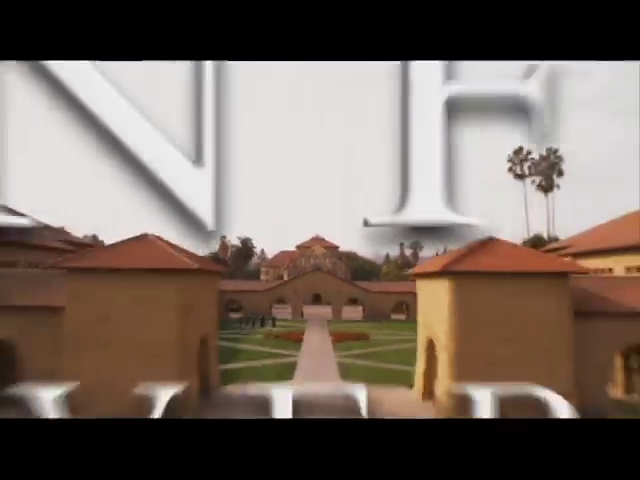
\includegraphics[width=0.78\textwidth]{lecture_02_figure_01.png}\caption{Các quy tắc sai phân hữu hạn và tổng Riemann được giữ lại trên bảng để dùng cho giới hạn liên tục về sau.}\lectureframe{00:04:20}\label{fig:l02-calculus-board}\end{figure}

Đây là những định nghĩa quen thuộc của giải tích. Tầm quan trọng của chúng ở đây nằm ở cách co giãn: \(\Delta x_i\) mang theo một lũy thừa của \(\Delta\sigma\), còn một tổng thì mang theo một lũy thừa nghịch khi trở thành tích phân.

\subsection{Các đầu mút Dirichlet và Neumann}

Phân tích Fourier trên một đoạn hữu hạn bắt đầu bằng một lựa chọn tại các đầu mút. Hai lựa chọn sẽ lặp lại nhiều lần.

\begin{align}
  \text{Dirichlet:}\qquad
  &x(0)=x(\pi)=0,
  \label{eq:l02-dirichlet}\\
  \text{Neumann:}\qquad
  &\left.\partial_\sigma x\right|_{\sigma=0}
   =
   \left.\partial_\sigma x\right|_{\sigma=\pi}
   =0.
  \label{eq:l02-neumann}
\end{align}

Một dây đàn vĩ cầm được giữ ở cả hai đầu cho ta bức tranh Dirichlet: độ dời của nó triệt tiêu tại các biên. Một hàm Neumann không nhất thiết triệt tiêu ở đó; nó chạm mỗi biên với độ dốc bằng không. Hai dạng đặc trưng ấy được thấy cùng nhau trên bảng.

\begin{figure}[H]\centering
  \begin{minipage}[t]{0.48\textwidth}\centering
    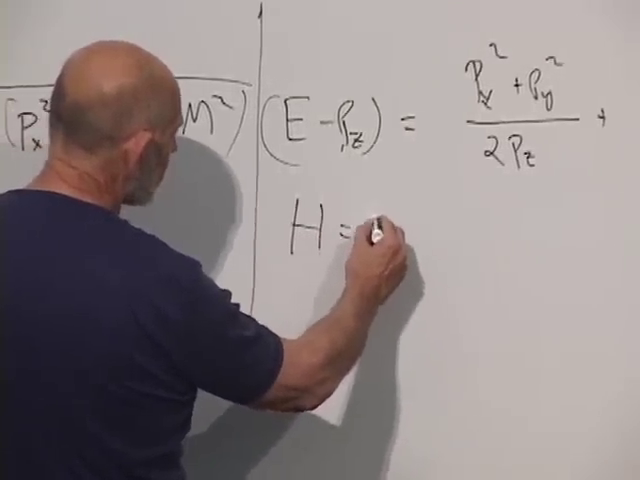
\includegraphics[width=\textwidth]{lecture_02_figure_02.png}\par\smallskip\footnotesize (a) Các biên dạng với đầu mút bị ghim và đầu mút phẳng.\end{minipage}\hfill
  \begin{minipage}[t]{0.48\textwidth}\centering
    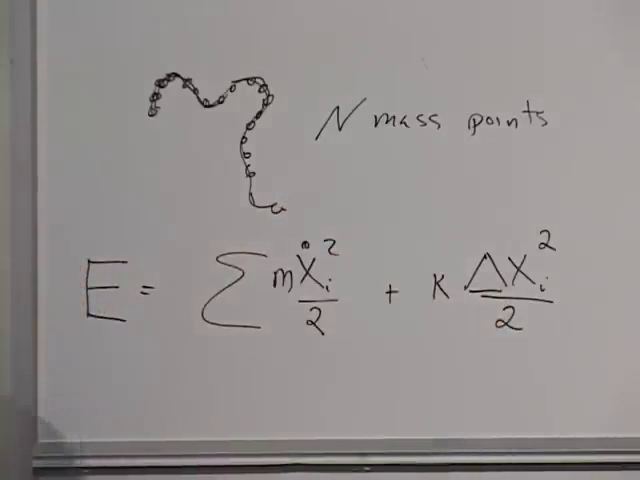
\includegraphics[width=\textwidth]{lecture_02_figure_03.png}\par\smallskip\footnotesize (b) Các vòng nhẹ trượt trên các cọc thẳng đứng.\end{minipage}\caption{Điều kiện biên dưới dạng hình dạng và dưới dạng cơ học. Cấu hình vòng trượt cho một đầu mút tự do một chuyển động ngang được xác định rõ ràng.}\lectureframe{00:08:50 and 00:12:15}\label{fig:l02-boundaries-board}\end{figure}

\begin{figure}[H]\centering
  \begin{adjustbox}{max width=\linewidth}\begin{tikzpicture}[>=Latex,thick,scale=0.92]
    \begin{scope}
      \draw[->] (0,0) -- (4.4,0) node[right] {\(\sigma\)};
      \draw[->] (0,-1.25) -- (0,1.35) node[above] {\(x\)};
      \draw[blue!70!black]
        (0,0) .. controls (0.8,1.1) and (1.4,1.0) .. (2.0,0)
        .. controls (2.7,-1.0) and (3.4,-0.8) .. (4.1,0);
      \fill (0,0) circle (0.06);
      \fill (4.1,0) circle (0.06);
      \node at (2.05,-1.65) {Dirichlet: \(x=0\)};
    \end{scope}
    \begin{scope}[xshift=5.8cm]
      \draw[->] (0,0) -- (4.4,0) node[right] {\(\sigma\)};
      \draw[->] (0,-1.25) -- (0,1.35) node[above] {\(x\)};
      \draw[orange!85!black]
        (0,0.65) .. controls (0.8,0.65) and (1.1,-0.9) .. (2.0,-0.9)
        .. controls (2.9,-0.9) and (3.2,0.55) .. (4.1,0.55);
      \draw[orange!85!black] (0,0.65) -- (0.45,0.65);
      \draw[orange!85!black] (3.65,0.55) -- (4.1,0.55);
      \node at (2.05,-1.65) {Neumann: \(\partial_\sigma x=0\)};
    \end{scope}
  \end{tikzpicture}\end{adjustbox}\caption{Giá trị được cố định đối với dữ liệu Dirichlet; độ dốc được cố định đối với dữ liệu Neumann.}\label{fig:l02-boundaries-redraw}\end{figure}

\begin{classroomqa}\audiencequestion{Một ống đàn organ hở hay kín có cho một ví dụ rõ ràng về một trong các điều kiện biên này không?\lecturetimestamp{00:09:19}}\lecturerresponse{Có thể, nhưng trước hết phải nói rõ đang khai triển biến âm học nào. Nhiễu loạn áp suất và độ dời dọc tuân theo những điều kiện lý tưởng hóa bổ sung lẫn nhau tại một đầu hở. Thay vì giải quyết câu hỏi bên lề ấy ngay trên bảng, hãy dùng mô hình vòng trượt: các vòng gần như không khối lượng có thể chuyển động thẳng đứng trên các cọc, nên các đầu mút của dây là tự do và bức tranh Neumann là trực tiếp.}\end{classroomqa}

\begin{classroomqa}\audiencequestion{Đồ thị có thể dựng đứng và chứa một bước nhảy đột ngột không?\lecturetimestamp{00:09:53}}\lecturerresponse{Phân tích Fourier cho phép những bước nhảy cô lập trong một hàm liên tục từng khúc. Một dây vật lý thì bị ràng buộc chặt hơn. Một bước nhảy làm các điểm lân cận mất liên thông và khiến đạo hàm theo không gian \(\partial_\sigma x\) trở nên kỳ dị trong năng lượng liên tục sẽ được suy ra bên dưới. Vì vậy ta chỉ giới hạn sự chú ý vào các biên dạng liên tục và khả vi.}\end{classroomqa}

\begin{classroomqa}\audiencequestion{Tại sao đầu hở của một ống, hay bất kỳ đầu tự do nào, lại phải thỏa một điều kiện biên?\lecturetimestamp{00:11:14}}\lecturerresponse{Ví dụ âm học phụ thuộc vào trường được chọn và đã được để ngỏ trong phần thảo luận. Ví dụ cơ học thì không. Một vòng rất nhẹ được tự do trượt nhưng vẫn gắn với đoạn dây cuối cùng. Ta sẽ suy ra điều kiện của nó từ định luật Newton thay vì giả sử trước: gia tốc hữu hạn ở đầu mút buộc độ dốc phải triệt tiêu.}\end{classroomqa}

\subsection{Các cơ sở Fourier}

Một khi kiểu điều kiện ở đầu mút đã được cố định, cơ sở Fourier tương ứng cũng được cố định. Trên \(0\leq\sigma\leq\pi\),

\begin{align}
  x_D(\sigma)
  &=
  \sum_{n=1}^{\infty}x_n\sin(n\sigma),
  \label{eq:l02-dirichlet-series}\\
  x_N(\sigma)
  &=
  \sum_{n=0}^{\infty}x_n\cos(n\sigma).
  \label{eq:l02-neumann-series}
\end{align}

Mọi hàm sin trong \eqref{eq:l02-dirichlet-series} đều triệt tiêu tại cả hai đầu mút. Mọi hàm cos trong \eqref{eq:l02-neumann-series} đều có đạo hàm ở đầu mút bằng không. Các cận dưới khác nhau là có lý do: \(\sin(0\sigma)=0\) không đóng góp gì, còn \(\cos(0\sigma)=1\) là mode hằng, hay mode không. Nó ghi lại giá trị trung bình của một hàm Neumann.

\begin{figure}[H]\centering
  \begin{minipage}[t]{0.48\textwidth}\centering
    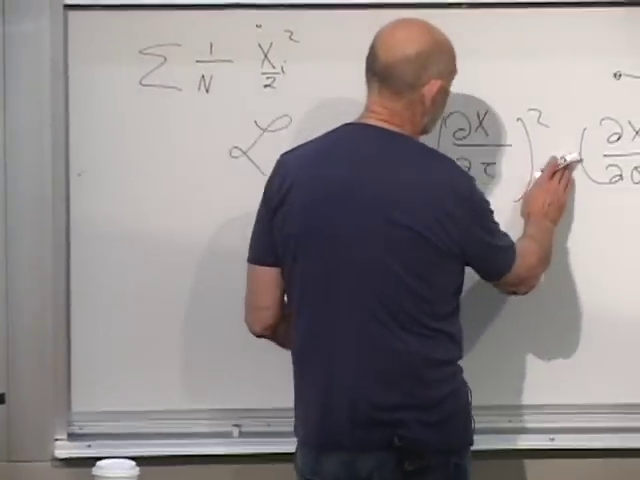
\includegraphics[width=\textwidth]{lecture_02_figure_04.png}\par\smallskip\footnotesize (a) Khai triển sin và cos.\end{minipage}\hfill
  \begin{minipage}[t]{0.48\textwidth}\centering
    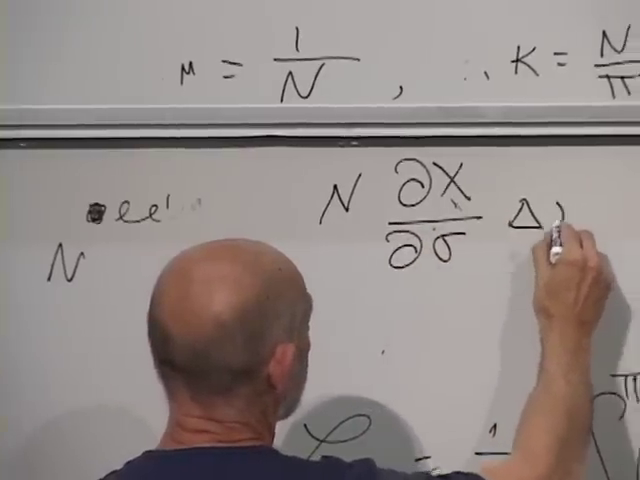
\includegraphics[width=\textwidth]{lecture_02_figure_05.png}\par\smallskip\footnotesize (b) Tính trực giao và mode hằng ngoại lệ.\end{minipage}\caption{Các tính chất Fourier sẽ được dùng về sau để chéo hóa dây.}\lectureframe{00:16:15 and 00:20:30}\label{fig:l02-fourier-board}\end{figure}

Phép lấy đạo hàm hoán đổi hai lớp này:

\begin{equation}
  \begin{aligned}
    \partial_\sigma\sin(n\sigma)&=n\cos(n\sigma),\\
    \partial_\sigma\cos(n\sigma)&=-n\sin(n\sigma).
  \end{aligned}
  \label{eq:l02-basis-derivatives}
\end{equation}

Do đó, đạo hàm của một chuỗi Dirichlet có tính chất Neumann, còn đạo hàm của một chuỗi Neumann có tính chất Dirichlet. Khi ấy tính trực giao khử các hạng chéo giữa những mode khác nhau:

\begin{align}
  \int_0^\pi\cos(n\sigma)\cos(m\sigma)\,d\sigma
  &=
  \frac{\pi}{2}\delta_{nm},
  && n,m\geq1,
  \label{eq:l02-cos-orthogonality}\\
  \int_0^\pi\sin(n\sigma)\sin(m\sigma)\,d\sigma
  &=
  \frac{\pi}{2}\delta_{nm},
  && n,m\geq1,
  \label{eq:l02-sin-orthogonality}\\
  \int_0^\pi 1\,d\sigma&=\pi .
  \label{eq:l02-zero-norm}
\end{align}

Dòng cuối cùng là chuẩn cos ngoại lệ ứng với \(n=m=0\). Một hằng số không được chuẩn hóa như một điều hòa khác không, và hệ số 2 ấy sẽ phân biệt mode khối tâm của dây với các mode nội tại của nó.

\subsection{Một công thức dao động tử cần nhớ}

Sau khi đổi tỷ lệ một tọa độ sao cho khối lượng cơ học của nó bằng một, một dao động tử theo định luật Hooke có

\begin{align}
  E_{\mathrm{osc}}
  &=
  \frac12\dot q^{\,2}
  +\frac12\omega^2q^2,
  \label{eq:l02-oscillator-energy}\\
  L_{\mathrm{osc}}
  &=
  \frac12\dot q^{\,2}
  -\frac12\omega^2q^2.
  \label{eq:l02-oscillator-lagrangian}
\end{align}

\begin{figure}[H]\centering
  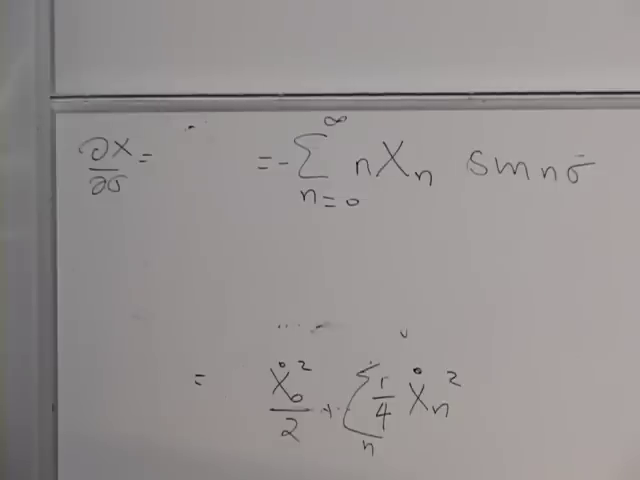
\includegraphics[width=0.68\textwidth]{lecture_02_figure_06.png}\caption{Năng lượng của dao động tử, được viết sao cho hệ số của \(q^2\) lập tức cho biết \(\omega^2\).}\lectureframe{00:24:00}\label{fig:l02-oscillator-board}\end{figure}

Về mặt cổ điển, \(\omega=\sqrt{\kappa/m}\); phép đổi tỷ lệ tọa độ đã đặt \(m=1\). Về mặt lượng tử,

\begin{equation}
  E_Q=\hbar\omega\left(Q+\frac12\right),
  \qquad Q=0,1,2,\ldots .
  \label{eq:l02-oscillator-spectrum}
\end{equation}

Khi xét khoảng cách mức, ta có thể trừ đi hạng trạng thái cơ bản chung và nói rằng mỗi lượng tử tốn \(\hbar\omega\). Ban đầu phép tính cho dây sẽ làm đúng như vậy và hoãn việc xử lý tổng năng lượng điểm không lại.

\begin{classroomqa}
\audiencequestion{Tần số của dao động tử được đọc ra từ công thức năng lượng như thế nào?\lecturetimestamp{00:23:21}}
\lecturerresponse{Trước khi đổi tỷ lệ, nó là \(\omega=\sqrt{\kappa/m}\). Khi khối lượng bằng một, hạng thế năng là \(\frac12\omega^2q^2\), nên hệ số bậc hai của nó chính là bình phương của tần số.}
\end{classroomqa}

\section{Điều gì làm cho một hệ hợp thành trở thành một hạt?}

Một dây có độ trải rộng và sẽ được mô hình hóa bằng nhiều phần tử liên kết với nhau. Vậy theo nghĩa nào một trong các trạng thái lượng tử của nó vẫn có thể là một hạt? Tính điểm không thể là tiêu chuẩn quyết định. Proton và neutron là những hệ hợp thành. Electron và photon đều đi kèm với một lớp bao bọc của trường lượng tử, dù chưa phân giải được cấu trúc con nội tại nào. Một điểm hình học cổ điển không có gì bao quanh không phải là hình ảnh đúng của một kích thích lượng tử.

Khối lượng và vị trí khối tâm cũng không đủ. Một hộp khí kín có cả hai. Một tách cà phê cũng có cả hai. Ta thường không gọi cái nào trong hai thứ ấy là một hạt. Tính không thể chia cắt cũng thất bại, vì proton là khả phân, và spin không phân biệt các hạt vi mô với các vật thể vĩ mô.

Tiêu chuẩn hữu ích là sự cô lập phổ. Đặt năng lượng nghỉ trên một trục đứng và hỏi cần bao nhiêu năng lượng để đạt tới một trạng thái nội tại khác. Electron không có một tháp các kích thích electron nằm ngay phía trên mà thí nghiệm có thể tiếp cận. Proton thì có các cộng hưởng, nhưng những cộng hưởng đầu tiên cần vài trăm MeV, một phần đáng kể của khối lượng proton. Các trạng thái đó tách nhau đủ xa để có thể nhận diện riêng rẽ.

Một tách cà phê thì ngược lại. Người ta có thể thêm một lượng năng lượng nhỏ tùy ý vào một mode âm thanh bước sóng dài, khẽ tác động lên một phân tử, hoặc tạo ra một phonon. Có rất nhiều trạng thái chen chúc trong một khoảng rất nhỏ. Ở các thang đo phòng thí nghiệm, chúng tạo thành một liên tục. Đây là sự phân biệt thực dụng giữa một hạt và \emph{một khối nhão}.

\begin{figure}[H]\centering
  \includegraphics[width=0.58\textwidth]{lecture_02_figure_07.png}\caption{Trục năng lượng thẳng đứng trên bảng khi so sánh một mức hạt cô lập với các kích thích dày đặc của vật chất thông thường.}\lectureframe{00:31:10}\label{fig:l02-spectrum-board}\end{figure}

\begin{figure}[H]\centering
  \begin{adjustbox}{max width=\linewidth}\begin{tikzpicture}[>=Latex,thick]
    \begin{scope}
      \draw[->] (0,0) -- (0,4.8) node[above] {energy};
      \draw[blue!70!black,line width=1.2pt] (-1.0,0.65) -- (1.0,0.65);
      \draw[blue!70!black,line width=1.2pt] (-1.0,3.65) -- (1.0,3.65);
      \node[right] at (1.05,0.65) {ground state};
      \node[right] at (1.05,3.65) {first internal excitation};
      \draw[<->] (0.65,0.75) -- (0.65,3.55)
        node[midway,right] {large gap};
      \node at (0,-0.55) {particle-like};
    \end{scope}
    \begin{scope}[xshift=7.0cm]
      \draw[->] (0,0) -- (0,4.8) node[above] {energy};
      \foreach \y in {0.55,0.69,0.82,0.94,1.05,1.15,1.24,1.32,1.39,1.45,
        1.51,1.57,1.63,1.70,1.78,1.87,1.97,2.09,2.22,2.36,2.51,2.67,2.84,
        3.02,3.21,3.41,3.62,3.84,4.07}
        \draw[orange!85!black] (-0.95,\y) -- (0.95,\y);
      \node[right] at (1.05,2.25) {dense phonon and internal states};
      \node at (0,-0.55) {macroscopic matter};
    \end{scope}
  \end{tikzpicture}\end{adjustbox}\caption{Sự cô lập phổ, chứ không phải tính điểm theo nghĩa đen, là tiêu chuẩn thao tác về hạt được dùng trong bài giảng.}\label{fig:l02-particle-redraw}\end{figure}

Tiêu chuẩn này biến câu hỏi triết học thành một phép tính. Hãy lượng tử hóa dây, tìm các mức năng lượng nội tại của nó, rồi xem xét khoảng cách giữa chúng. Nếu trạng thái kích thích đầu tiên của dây nằm gần thang Planck trong khi trạng thái cơ bản quan sát được là nhẹ, thì khe đó vượt quá năng lượng của các máy gia tốc hiện nay hơn 20 bậc độ lớn. Khi ấy dây hành xử như một hạt cơ bản trong toàn bộ miền có thể tiếp cận.

\begin{classroomqa}\audiencequestion{Hành vi hạt có chỉ đơn thuần là vấn đề thang quan sát không? Nếu ta phóng to đủ mức, các mức có thôi tách biệt nữa không?\lecturetimestamp{00:33:33}}\lecturerresponse{Việc nhìn đủ kỹ có thể cho thấy một đối tượng có nhiều thành phần cấu tạo, nhưng nó không xóa phổ đi. So sánh thích hợp là giữa độ phân giải năng lượng của thí nghiệm và khe tới kích thích nội tại đầu tiên. Một đối tượng hợp thành vẫn có thể mang tính hạt khi khe đó là rất lớn.}\end{classroomqa}

\begin{classroomqa}\audiencequestion{Tại sao một dây đàn vĩ cầm thông thường lại không phải là một hạt?\lecturetimestamp{00:34:37}}\lecturerresponse{Một lượng tử dao động mang năng lượng nhỏ đến mức không thể đo được so với năng lượng nghỉ của sợi dây vĩ mô. Vì vậy, nhiều trạng thái lượng tử chen vừa vào một khoảng tương đối rất nhỏ. Nó thuộc về phía dày đặc của phép so sánh phổ, chứ không phải phía cô lập.}\end{classroomqa}

\begin{classroomqa}\audiencequestion{Photon và electron có phải là hạt điểm không, nếu xung quanh chúng có các thăng giáng ảo của trường lượng tử?\lecturetimestamp{00:35:40}}\lecturerresponse{Từ cổ điển \emph{điểm} đang phải gánh quá nhiều ý nghĩa. Electron và photon vật lý là các kích thích trường đã được hiệu chỉnh, nhưng thực nghiệm chưa tìm thấy ở bên nào cấu trúc thành phần nội tại hay nhân tử dạng hữu hạn. Điều quan trọng đối với lập luận hiện tại là không bên nào có một tháp dày đặc các trạng thái nội tại gần suy biến.\editorialnote{Bài giảng liên hệ mômen từ dị thường của electron với một độ mờ lượng tử có thể đo được. Theo thuật ngữ hiện đại, mômen dị thường là một hiệu ứng hiệu chỉnh bức xạ, chứ không phải bằng chứng về một bán kính electron hữu hạn đã được phân giải. Theo quy ước, dạng điểm có nghĩa là chưa phát hiện được cấu trúc con nội tại hay nhân tử dạng nào xuống tới thang đã được kiểm nghiệm.}}\end{classroomqa}

\begin{classroomqa}\audiencequestion{Kích thước của photon có phụ thuộc vào tần số của nó không?\lecturetimestamp{00:36:49}}\lecturerresponse{Bước sóng của nó thì chắc chắn có phụ thuộc. Điều đó khác với một kích thước thành phần nội tại. Việc thay đổi tần số làm thay đổi gói sóng và bước sóng, chứ không phải một bán kính nội tại của photon đã được phân giải.}\end{classroomqa}

\section{Cơ học ngang chính xác ở xung lượng lớn}

Bây giờ ta quay lại khó khăn tương đối tính. Một cây gậy quay nhanh không thể được xử lý phi tương đối tính chỉ bằng cách đặt khối tâm của nó đứng yên. Các đầu của nó vẫn chuyển động tương đối tính đối với nhau. Xấp xỉ phi tương đối tính thất bại vì chuyển động tương đối nội bộ.

Tuy nhiên, có một giới hạn khác. Chọn một trục \(z\) và thực hiện một phép boost cho toàn bộ hệ tới một xung lượng dọc dương rất lớn \(P_z\). Giữ xung lượng ngang của nó

\begin{equation}
  p_\perp^2=p_x^2+p_y^2
\end{equation}

hữu hạn. Khi đó phép chiếu theo phương ngang có dạng Hamilton phi tương đối tính một cách chính xác trong giới hạn \(P_z\to\infty\), ngay cả khi chuyển động nội bộ trước phép boost là tương đối tính.

\begin{classroomqa}
\audiencequestion{Động lượng vô hạn có nghĩa là hệ có khối lượng thực sự đạt tới tốc độ ánh sáng không?\lecturetimestamp{00:40:43}}
\lecturerresponse{Không có phép boost hữu hạn nào đạt tới tốc độ ấy. Người ta xây dựng các đại lượng có giới hạn xác định khi \(P_z\) trở nên lớn tùy ý. Cụm từ này chỉ một quy trình lấy giới hạn, không phải một trạng thái vật lý hữu hạn với \(v=c\).}
\end{classroomqa}

\begin{classroomqa}
\audiencequestion{Phải chọn trục nào, và điều gì xảy ra nếu vật quay quanh hoặc ngang qua trục đó?\lecturetimestamp{00:41:14}}
\lecturerresponse{Có thể chọn bất kỳ trục nào và boost toàn bộ hệ dọc theo trục ấy. Điều còn lại dưới dạng cơ học tường minh là hình chiếu lên mặt phẳng vuông góc. Một thanh quay có thể trông bị co ngắn lại hoặc quét qua mặt phẳng đó, nhưng hình chiếu ngang của nó có dạng phi tương đối tính.}
\end{classroomqa}

Dây có thêm một tính chất khiến biểu diễn này đặc biệt mạnh. Trong chuẩn light-front, các tọa độ nội tại dọc của nó không phải là những dao động tử độc lập. Các ràng buộc xác định chúng từ chuyển động ngang. Vì vậy, chỉ cần biết cấu hình ngang của dây là đủ để tái dựng các bậc tự do vật lý.

\begin{classroomqa}
\audiencequestion{Việc không có một tọa độ dọc độc lập có nghĩa là dây chỉ đơn thuần bị kẹt trong một lớp mỏng hay không?\lecturetimestamp{00:42:26}}
\lecturerresponse{Sự co Lorentz quả thật làm cho độ dài dọc của nó nhỏ trong hệ quy chiếu được boost, nhưng phát biểu ở đây còn mạnh hơn. Mọi chuyển động dọc còn lại đều bị chuyển động ngang ràng buộc; không thể được chỉ định độc lập.}
\end{classroomqa}

\begin{classroomqa}
\audiencequestion{Sự quy giản này về dữ liệu ngang có liên quan đến nguyên lý toàn ảnh không?\lecturetimestamp{00:43:12}}
\lecturerresponse{Nó liên hệ chặt chẽ với mạch tư duy đã dẫn tới các ý tưởng toàn ảnh, mặc dù theo đuổi mối liên hệ ấy sẽ đưa ta ra khỏi phép tính hiện tại. Ở đây nó chỉ dùng để biện minh cho việc làm việc với cấu hình ngang của dây.}
\end{classroomqa}

\subsection{Trừ phần do boost và đổi thang thời gian}

Gọi \(M\) là khối lượng bất biến của toàn hệ, bao gồm khối lượng các thành phần, động năng và năng lượng liên kết. Trong đơn vị \(c=1\),

\begin{equation}
  E=\sqrt{P_z^2+p_\perp^2+M^2}.
  \label{eq:l02-relativistic-energy}
\end{equation}

Với \(P_z\) lớn hơn nhiều so với \(p_\perp\) và \(M\),

\begin{equation}
  E
  =
  P_z+\frac{p_\perp^2+M^2}{2P_z}
  +O(P_z^{-3}).
  \label{eq:l02-large-pz}
\end{equation}

\begin{figure}[H]
  \centering
  \includegraphics[width=0.76\textwidth]{lecture_02_figure_08.png}
  \caption{Khai triển đầy đủ theo large-\(P_z\), trong đó động lượng ngang và khối lượng bất biến được giữ lại.}
  \lectureframe{00:47:30}
  \label{fig:l02-large-pz-board}
\end{figure}

Hạng dẫn đầu rất lớn, nhưng nó không mang thông tin nào về trạng thái nội. Trong một quá trình bảo toàn \(P_z\), chẳng hạn một nguyên tử được boost chuyển giữa các mức nội mà không thay đổi tổng động lượng dọc của nó, hạng ấy triệt tiêu khỏi mọi hiệu năng lượng. Vì vậy ta khảo sát

\begin{equation}
  E-P_z=\frac{p_\perp^2+M^2}{2P_z}+O(P_z^{-3}).
  \label{eq:l02-residual-energy}
\end{equation}

Mẫu số có một ý nghĩa vật lý. Vì Hamiltonian sinh ra sự tiến hóa theo thời gian, năng lượng dư nhỏ cho thấy sự tiến hóa nội có vẻ chậm trong thời gian phòng thí nghiệm. Đó là giãn thời gian. Để giữ lại chuyển động nội, ta đưa vào một tham số tiến hóa đã đổi thang \(\tau\), hoặc tương đương nhân Hamiltonian dư với \(P_z\):

\begin{equation}
  H_\perp
  \equiv
  \lim_{P_z\to\infty}P_z(E-P_z)
  =
  \frac12p_\perp^2+\frac12M^2.
  \label{eq:l02-transverse-hamiltonian}
\end{equation}

\begin{figure}[H]
  \centering
  \begin{minipage}[t]{0.48\textwidth}
    \centering
    \includegraphics[width=\textwidth]{lecture_02_figure_09.png}
    \par\smallskip\footnotesize (a) \(H=i\partial_t\) và sự tiến hóa nội bị làm chậm.
  \end{minipage}\hfill
  \begin{minipage}[t]{0.48\textwidth}
    \centering
    \includegraphics[width=\textwidth]{lecture_02_figure_10.png}
    \par\smallskip\footnotesize (b) Hamiltonian ngang hữu hạn sau khi đổi thang thời gian.
  \end{minipage}
  \caption{Từ năng lượng dư đã bị giãn thời gian đến một Hamiltonian hai chiều hữu hạn.}
  \lectureframe{00:49:20 and 00:52:40}
  \label{fig:l02-lightfront-board}
\end{figure}

Đây chính xác là dạng của một hạt khối lượng đơn vị chuyển động trong hai chiều: động năng \(p_\perp^2/2\) cộng với một năng lượng nội \(M^2/2\). Điểm khác thường là bình phương. Trong mô tả này, đại lượng đóng vai trò năng lượng nghỉ hay năng lượng liên kết tỉ lệ với bình phương khối lượng bất biến.\editorialnote{Với các biến light-front thông thường \(P^\pm=(E\pm P_z)/\sqrt2\), hệ thức vỏ khối lượng chính xác là \(2P^+P^-=p_\perp^2+M^2\). Phương trình \eqref{eq:l02-transverse-hamiltonian} là cách chuẩn hóa large-\(P_z\) của bài giảng cho cùng một hệ thức bất biến.}

\begin{classroomqa}
\audiencequestion{Các động lượng dọc của từng phần riêng lẻ trong một hệ hợp thành đã đi đâu?\lecturetimestamp{00:51:30}}
\lecturerresponse{Đối với một vật hợp thành tổng quát, ta phải giữ lại các tỉ phần của tổng \(P_z\) do các thành phần của nó mang. Công thức trên dùng tổng động lượng của khối tâm. Lý thuyết dây là đặc biệt vì các ràng buộc của nó xác định chuyển động dọc tương đối từ các bậc tự do ngang, nên không cần thêm một dao động tử dọc độc lập nào.}
\end{classroomqa}

\section{Một dây mở rời rạc}

Dây được boost giờ đây tường minh chỉ chuyển động trong mặt phẳng ngang. Gọi hai tọa độ của nó là \(X\) và \(Y\), và trước hết xấp xỉ nó bằng \(N\) chất điểm được nối với nhau bởi \(N-1\) lò xo. Nếu \(\mu\) là khối lượng tương tự của mỗi điểm và \(k\) là hằng số đàn hồi giữa các láng giềng gần, thì năng lượng là

\begin{equation}
  E_N
  =
  \sum_i
  \left[
    \frac{\mu}{2}
    \left(\dot X_i^2+\dot Y_i^2\right)
    +
    \frac{k}{2}
    \left((\Delta X_i)^2+(\Delta Y_i)^2\right)
  \right].
  \label{eq:l02-discrete-energy}
\end{equation}

Mỗi hạng \(X\) đều có một hạng \(Y\) giống hệt, vì mặt phẳng ngang có hai phương. Chỉ số \(i\) gắn nhãn một điểm dọc theo chuỗi; nó không phải là một tọa độ không gian.

\begin{figure}[H]
  \centering
  \begin{minipage}[t]{0.48\textwidth}
    \centering
    \includegraphics[width=\textwidth]{lecture_02_figure_11.png}
    \par\smallskip\footnotesize (a) Chuỗi hạt và năng lượng rời rạc của nó.
  \end{minipage}\hfill
  \begin{minipage}[t]{0.48\textwidth}
    \centering
    \includegraphics[width=\textwidth]{lecture_02_figure_12.png}
    \par\smallskip\footnotesize (b) Quy luật tỉ lệ large-\(N\) của \(\mu\) và \(k\).
  \end{minipage}
  \caption{Dây mở được điều chuẩn trước khi lấy giới hạn liên tục.}
  \lectureframe{00:57:42 and 01:02:40}
  \label{fig:l02-chain-board}
\end{figure}

\begin{figure}[H]
  \centering
  \begin{adjustbox}{max width=\linewidth}
  \begin{tikzpicture}[>=Latex,thick]
    \foreach \i in {0,...,8} {
      \coordinate (p\i) at ({1.05*\i},{0.30*sin(55*\i)});
      \filldraw[white] (p\i) circle (0.10);
      \draw (p\i) circle (0.10);
    }
    \foreach \i in {0,...,7} {
      \pgfmathtruncatemacro{\j}{\i+1}
      \draw[decorate,decoration={zigzag,segment length=4pt,amplitude=2pt}]
        (p\i) -- (p\j);
    }
    \node[above=0.35cm of p0] {\(i=0\)};
    \node[above=0.35cm of p8] {\(i=N-1\)};
    \draw[<->] (0,-1.15) -- (8.4,-1.15)
      node[midway,below] {\(0\leq\sigma\leq\pi\)};
    \node at (4.2,1.25)
      {\(\mu=1/N,\quad k=N/\pi^2,\quad\Delta\sigma=\pi/N\)};
  \end{tikzpicture}
  \end{adjustbox}
  \caption{Một hình ảnh điều chuẩn rõ ràng. Khi chuỗi được tinh luyện hơn, các điểm trở nên nhẹ hơn còn các lò xo vi mô trở nên cứng hơn.}
  \label{fig:l02-chain-redraw}
\end{figure}

Tham số \(\sigma\) gắn nhãn vị trí dọc theo chuỗi. Việc chọn \(0\leq\sigma\leq\pi\) là một quy ước, không phải một phép đo độ dài vật lý. Nó nhắc ta rằng dây có hai đầu mút. Sau này, một dây kín sẽ được gắn nhãn tuần hoàn trên \(0\leq\sigma<2\pi\).

Giới hạn liên tục phải giữ cho cơ học tập thể là hữu hạn. Nếu giữ cố định khối lượng mỗi hạt, tổng khối lượng tương tự sẽ phân kỳ, nên hãy chọn

\begin{equation}
  \mu=\frac{1}{N}.
  \label{eq:l02-mu-scaling}
\end{equation}

Khi đó \(N\mu=1\). Đây không phải là khối lượng nghỉ tương đối tính \(M\); nó là hệ số quán tính trong mô hình tương tự ngang.

Các lò xo mắc nối tiếp trở nên mềm hơn khi số lượng của chúng tăng lên. Để bảo toàn một độ cứng hữu hạn cho toàn chuỗi, mỗi lò xo vi mô phải trở nên cứng hơn:

\begin{equation}
  k=\frac{N}{\pi^2}
  =\frac{1}{\pi\,\Delta\sigma}.
  \label{eq:l02-k-scaling}
\end{equation}

Chỉ \(k\propto N\) là thiết yếu. Hệ số \(\pi^2\) là một chuẩn hóa được chọn để loại bỏ các hệ số \(\pi\) lạc lõng khỏi các công thức liên tục.

\begin{classroomqa}
\audiencequestion{Liệu \(\mu\) có phải là khối lượng nghỉ vật lý của mỗi điểm trên dây không?\lecturetimestamp{01:10:34}}
\lecturerresponse{Không. Nó là khối lượng tương tự phi tương đối tính xuất hiện trong chuỗi ngang. Gọi nó là \(M\) sẽ gây nhầm lẫn với khối lượng nghỉ bất biến của toàn trạng thái dây tương đối tính. Vai trò duy nhất của nó ở đây là tạo ra quán tính liên tục đúng.}
\end{classroomqa}

\section{Hệ sóng liên tục}

Hãy áp dụng các quy tắc đã chuẩn bị ở phần đầu. Vì \(1/N=\Delta\sigma/\pi\),

\begin{align}
  \sum_i\frac{\mu}{2}\dot X_i^2
  &=
  \frac{1}{2\pi}
  \sum_i\dot X_i^2\,\Delta\sigma
  \longrightarrow
  \frac{1}{2\pi}
  \int_0^\pi
  \left(\partial_\tau X\right)^2d\sigma ,
  \label{eq:l02-kinetic-limit}\\
  \sum_i\frac{k}{2}(\Delta X_i)^2
  &\longrightarrow
  \frac{1}{2\pi}
  \int_0^\pi
  \left(\partial_\sigma X\right)^2d\sigma .
  \label{eq:l02-potential-limit}
\end{align}

Đối với dòng thứ hai, dùng \(\Delta X_i=\partial_\sigma X\,\Delta\sigma\) cùng với \(k=1/(\pi\Delta\sigma)\). Phép tính tương tự cũng áp dụng cho \(Y\).

\begin{figure}[H]
  \centering
  \begin{minipage}[t]{0.48\textwidth}
    \centering
    \includegraphics[width=\textwidth]{lecture_02_figure_13.png}
    \par\smallskip\footnotesize (a) Các phép thay tổng bằng tích phân và sai phân bằng đạo hàm.
  \end{minipage}\hfill
  \begin{minipage}[t]{0.48\textwidth}
    \centering
    \includegraphics[width=\textwidth]{lecture_02_figure_14.png}
    \par\smallskip\footnotesize (b) Biểu thức năng lượng liên tục hoàn chỉnh.
  \end{minipage}
  \caption{Chuỗi rời rạc trở thành một trường trên khoảng \(\sigma\).}
  \lectureframe{01:05:40 and 01:07:00}
  \label{fig:l02-continuum-board}
\end{figure}

Năng lượng và Lagrangian thu được là

\begin{align}
  E
  &=
  \frac{1}{2\pi}
  \int_0^\pi d\sigma\,
  \left[
    (\partial_\tau X)^2+(\partial_\tau Y)^2\right.\notag\\[-0.25em]
  &\hspace{6.5em}\left.
    +(\partial_\sigma X)^2+(\partial_\sigma Y)^2
  \right],
  \label{eq:l02-continuum-energy}\\
  L
  &=
  \frac{1}{2\pi}
  \int_0^\pi d\sigma\,
  \left[
    (\partial_\tau X)^2+(\partial_\tau Y)^2\right.\notag\\[-0.25em]
  &\hspace{6.5em}\left.
    -(\partial_\sigma X)^2-(\partial_\sigma Y)^2
  \right].
  \label{eq:l02-continuum-lagrangian}
\end{align}

\begin{figure}[H]
  \centering
  \includegraphics[width=0.78\textwidth]{lecture_02_figure_15.png}
  \caption{Lagrangian liên tục với các hạng động năng và kéo dãn mang dấu đối nhau.}
  \lectureframe{01:08:48}
  \label{fig:l02-lagrangian-board}
\end{figure}

Nếu ta đổi tên \(\sigma\) thành một tọa độ không gian thông thường và \(X\) thành một trường \(\phi\), thì đây là năng lượng và Lagrangian của một trường sóng một chiều. Lấy biến phân \eqref{eq:l02-continuum-lagrangian} cho

\begin{equation}
  \left(\partial_\tau^2-\partial_\sigma^2\right)X=0,
  \qquad
  \left(\partial_\tau^2-\partial_\sigma^2\right)Y=0.
  \label{eq:l02-wave-equation}
\end{equation}

Không có gì trong lập luận trước mắt buộc ta phải giải trực tiếp các phương trình này. Bức tranh hữu ích đơn giản là các sóng truyền sang trái và sang phải dọc theo dây và phản xạ tại các đầu mút. Phản xạ Dirichlet đảo dấu độ dời; phản xạ Neumann giữ nguyên dấu đó.

\begin{classroomqa}
\audiencequestion{Chính xác thì biến thời gian \(\tau\) là gì?\lecturetimestamp{01:08:54}}
\lecturerresponse{Đó là thời gian đã được đổi thang dùng để theo dõi chuyển động nội trong mô tả large-\(P_z\). Một chiếc đồng hồ được boost cùng hệ chạy chậm so với thời gian phòng thí nghiệm; \(\tau\) loại bỏ sự giãn ấy để các dao động nội giữ được một tốc độ hữu hạn. Đối với cơ học ngang này, có thể đơn giản coi nó là thời gian.\editorialnote{Bài giảng gọi \(\tau\) một cách không chặt chẽ là thời gian riêng. Đối với một dây mở rộng, tham số tiến hóa light-front chính xác là một thời gian đã đổi thang sau khi cố định chuẩn, chứ không phải một thời gian riêng bất biến duy nhất được mọi điểm cùng chia sẻ. Luận điểm về giãn thời gian được nhắm đến không thay đổi.}}
\end{classroomqa}

Khi khối tâm đứng yên trong mặt phẳng ngang, phần nội của \eqref{eq:l02-continuum-energy}, theo chuẩn hóa của \eqref{eq:l02-transverse-hamiltonian}, tỉ lệ với \(M^2\). Đó là lý do lượng tử hóa hệ sóng có vẻ thông thường này sẽ làm lộ ra phổ khối lượng tương đối tính.

\begin{classroomqa}
\audiencequestion{\(P_z(E-P_z)\) có tên gọi nào không?\lecturetimestamp{01:11:00}}
\lecturerresponse{Nó thường được gọi là năng lượng light-cone hay light-front. Light front mô tả thích hợp hơn siêu phẳng không được dùng làm mặt tiến hóa; thuật ngữ truyền thống không quan trọng đối với phép tính.}
\end{classroomqa}

\begin{classroomqa}
\audiencequestion{Từ cone ở đây có chỉ nón ánh sáng không-thời gian quen thuộc, và Dirac có đưa ra thuật ngữ này không?\lecturetimestamp{01:11:17}}
\lecturerresponse{Cách dựng bằng tọa độ null có thể được vẽ với các trục 45 độ, nhưng mặt tiến hóa ở đây là một light front chứ không phải toàn bộ nón đang nở ra. Dirac đã phát triển các dạng tương ứng của động lực học tương đối tính; câu hỏi lịch sử về tên gọi được để ngỏ và không ảnh hưởng đến các phương trình.}
\end{classroomqa}

\section{Vì sao đầu mút tự do là Neumann}

Giờ đây ta có thể suy ra thay vì chỉ giả định điều kiện ở đầu mút. Định luật Newton là hợp lệ vì cơ học ngang sau boost có đúng dạng phi tương đối tính. Một điểm khối lượng ở bên trong bị kéo bởi các lò xo ở cả hai phía. Điểm cuối cùng chỉ bị kéo bởi lò xo nối nó với điểm láng giềng.

\begin{classroomqa}
\audiencequestion{Tại sao ta được phép dùng định luật Newton trong khi đang bàn về một dây tương đối tính?\lecturetimestamp{01:14:52}}
\lecturerresponse{Ta không áp dụng cơ học Newton cho chuyển động không-thời gian đầy đủ, chưa boost. Ta áp dụng nó cho các biến ngang trong mô tả động lượng vô hạn, mà Hamiltonian của nó có đúng dạng phi tương đối tính.}
\end{classroomqa}

Tại đầu mút phải, định luật Hooke cho, tùy theo quy ước hướng,

\begin{equation}
  F_{\mathrm{end}}
  =
  -k\,\Delta X
  =
  -\frac{1}{\pi\Delta\sigma}
   \left(\partial_\sigma X\,\Delta\sigma\right)
  =
  -\frac{1}{\pi}\partial_\sigma X .
  \label{eq:l02-endpoint-force}
\end{equation}

\begin{figure}[H]
  \centering
  \begin{minipage}[t]{0.48\textwidth}
    \centering
    \includegraphics[width=\textwidth]{lecture_02_figure_16.png}
    \par\smallskip\footnotesize (a) Lực ở đầu mút tỉ lệ với độ dốc cục bộ.
  \end{minipage}\hfill
  \begin{minipage}[t]{0.48\textwidth}
    \centering
    \includegraphics[width=\textwidth]{lecture_02_figure_17.png}
    \par\smallskip\footnotesize (b) Điều kiện gia tốc hữu hạn.
  \end{minipage}
  \caption{Phép suy ra điều kiện biên đầu tự do bằng định luật Newton.}
  \lectureframe{01:18:20 and 01:20:10}
  \label{fig:l02-neumann-board}
\end{figure}

Phương trình Newton cho điểm cuối là

\begin{equation}
  \mu\,\partial_\tau^2X=F_{\mathrm{end}},
  \qquad
  \mu=\frac1N=\frac{\Delta\sigma}{\pi}.
  \label{eq:l02-endpoint-newton}
\end{equation}

Kết hợp \eqref{eq:l02-endpoint-force} và \eqref{eq:l02-endpoint-newton},

\begin{equation}
  \partial_\sigma X
  =
  -\Delta\sigma\,\partial_\tau^2X
  \quad\text{at the right endpoint},
  \label{eq:l02-endpoint-scaling}
\end{equation}

với dấu của lực đảo ngược ở đầu mút trái. Nếu \(\partial_\sigma X\) tiến tới một hằng số khác không trong khi \(\Delta\sigma\to0\), thì gia tốc ở đầu mút sẽ phân kỳ như \(N\). Vì vậy, một giới hạn liên tục hợp lý với gia tốc hữu hạn đòi hỏi

\begin{equation}
  \left.\partial_\sigma X\right|_{0,\pi}=0,
  \qquad
  \left.\partial_\sigma Y\right|_{0,\pi}=0.
  \label{eq:l02-open-neumann}
\end{equation}

\begin{figure}[H]
  \centering
  \begin{adjustbox}{max width=\linewidth}
  \begin{tikzpicture}[>=Latex,thick,scale=1.0]
    \coordinate (a) at (0,0);
    \coordinate (b) at (4.5,0.75);
    \filldraw[white] (a) circle (0.12);
    \draw (a) circle (0.12);
    \filldraw[white] (b) circle (0.12);
    \draw (b) circle (0.12);
    \draw[decorate,decoration={zigzag,segment length=6pt,amplitude=3pt}]
      (a) -- (b);
    \draw[dashed] (a) -- (0,-1.2);
    \draw[dashed] (b) -- (4.5,-1.2);
    \draw[<->] (4.85,0) -- (4.85,0.75)
      node[midway,right] {\(\Delta X\)};
    \draw[->,red!70!black] (b) -- (5.75,0.95)
      node[right] {\(F_{\rm end}=-k\Delta X\)};
    \node[below] at (0,-1.2) {\(N-1\)};
    \node[below] at (4.5,-1.2) {\(N\)};
    \node at (2.5,-2.0)
      {\(\mu\ddot X=-k\Delta X
      \ \Longrightarrow\
      \partial_\sigma X=-\Delta\sigma\,\ddot X\to0\)};
  \end{tikzpicture}
  \end{adjustbox}
  \caption{Điểm cuối cùng có khối lượng triệt tiêu trong giới hạn điều chuẩn. Gia tốc hữu hạn chỉ có thể có khi độ dốc ở đầu mút triệt tiêu.}
  \label{fig:l02-neumann-redraw}
\end{figure}

Lập luận tương tự ở cả hai đầu và trong cả hai phương ngang cho ra các điều kiện biên Neumann đối với một dây mở tự do.

\section{Các mode chuẩn của dây mở}

Bây giờ ta đã có một hệ cổ điển hoàn chỉnh: một Lagrangian và các điều kiện biên của nó. Việc lượng tử hóa trở nên đơn giản sau khi phân tích Fourier. Vì các đầu mút thỏa điều kiện Neumann,

\begin{align}
  X(\sigma,\tau)
  &=
  \sum_{n=0}^{\infty}X_n(\tau)\cos(n\sigma),
  \label{eq:l02-X-expansion}\\
  Y(\sigma,\tau)
  &=
  \sum_{n=0}^{\infty}Y_n(\tau)\cos(n\sigma).
  \label{eq:l02-Y-expansion}
\end{align}

Các hàm cos chứa toàn bộ sự phụ thuộc theo \(\sigma\). Các hệ số chứa toàn bộ sự phụ thuộc theo thời gian; dây dao động vì \(X_n(\tau)\) và \(Y_n(\tau)\) thay đổi.

\begin{figure}[H]
  \centering
  \includegraphics[width=0.78\textwidth]{lecture_02_figure_18.png}
  \caption{Khai triển mode Neumann đặt cạnh quy tắc trực giao sẽ rút gọn các tổng kép.}
  \lectureframe{01:21:45}
  \label{fig:l02-mode-expansion-board}
\end{figure}

\subsection{Hạng động năng và mode không}

Lấy đạo hàm theo thời gian, ta được

\begin{equation}
  \partial_\tau X
  =
  \sum_{n=0}^{\infty}\dot X_n(\tau)\cos(n\sigma).
  \label{eq:l02-time-mode}
\end{equation}

Bình phương cho ra một tổng kép theo \(n\) và \(m\), nhưng \eqref{eq:l02-cos-orthogonality} loại bỏ mọi hạng có \(n\neq m\). Tách riêng mode hằng,

\begin{equation}
  \frac{1}{2\pi}\int_0^\pi
  (\partial_\tau X)^2\,d\sigma
  =
  \frac12\dot X_0^{\,2}
  +
  \frac14\sum_{n=1}^{\infty}\dot X_n^{\,2}.
  \label{eq:l02-mode-kinetic}
\end{equation}

\begin{figure}[H]
  \centering
  \includegraphics[width=0.76\textwidth]{lecture_02_figure_19.png}
  \caption{Tích phân trực giao rút gọn tổng kép của động năng thành mode không cộng với một tổng chéo.}
  \lectureframe{01:29:10}
  \label{fig:l02-mode-kinetic-board}
\end{figure}

Hệ số hằng là vị trí trung bình,

\begin{equation}
  X_0(\tau)=\frac1\pi\int_0^\pi X(\sigma,\tau)\,d\sigma ,
  \label{eq:l02-center-of-mass}
\end{equation}

và tương tự đối với \(Y_0\). Với mật độ khối lượng tương tự phân bố đều, đây là các tọa độ khối tâm. Chúng có động năng nhưng không có lực phục hồi: toàn bộ dây được tự do chuyển động trong mặt phẳng ngang.

\subsection{Hạng kéo dãn và các tần số dao động tử}

Lấy đạo hàm theo không gian, ta được

\begin{equation}
  \partial_\sigma X
  =
  -\sum_{n=1}^{\infty}nX_n(\tau)\sin(n\sigma).
  \label{eq:l02-spatial-mode}
\end{equation}

Mode không biến mất vì phép tịnh tiến đồng đều không kéo dãn dây. Dùng tính trực giao của sin,

\begin{equation}
  \frac{1}{2\pi}\int_0^\pi
  (\partial_\sigma X)^2\,d\sigma
  =
  \frac14\sum_{n=1}^{\infty}n^2X_n^{\,2}.
  \label{eq:l02-mode-potential}
\end{equation}

\begin{figure}[H]
  \centering
  \includegraphics[width=0.76\textwidth]{lecture_02_figure_20.png}
  \caption{Lấy đạo hàm chuỗi cos cho tổng kép các sin; tính trực giao lại áp đặt \(n=m\).}
  \lectureframe{01:31:40}
  \label{fig:l02-mode-potential-board}
\end{figure}

Vì vậy, Lagrangian của phần \(X\) là

\begin{equation}
  L_X
  =
  \frac12\dot X_0^{\,2}
  +
  \frac14\sum_{n=1}^{\infty}
  \left(
    \dot X_n^{\,2}-n^2X_n^{\,2}
  \right),
  \label{eq:l02-X-lagrangian}
\end{equation}

với một biểu thức y hệt cho \(Y\). Năng lượng tương ứng có dấu cộng trước \(n^2X_n^2\). Mỗi mode khác không là một dao động tử điều hòa độc lập, và so sánh với \eqref{eq:l02-oscillator-lagrangian} cho

\begin{equation}
  \omega_n=n,
  \qquad n=1,2,3,\ldots .
  \label{eq:l02-mode-frequency}
\end{equation}

\begin{figure}[H]
  \centering
  \includegraphics[width=0.80\textwidth]{lecture_02_figure_21.png}
  \caption{Lagrangian dao động tử đã tách rời và kết luận
  \(\omega_n=n\), với tháp \(Y\) giống hệt được chỉ ra bên dưới.}
  \lectureframe{01:35:50}
  \label{fig:l02-oscillator-modes-board}
\end{figure}

Các mode chuẩn đơn giản chính là các họa âm của dây. Họa âm thứ nhất dao động chậm, họa âm thứ hai có tần số gấp đôi, họa âm thứ ba gấp ba, v.v. Chính tính trực giao ngăn không cho một họa âm ghép với họa âm khác trong lý thuyết tự do.

\begin{classroomqa}
\audiencequestion{Dao động tử \(n=0\)
đã đi đâu?\lecturetimestamp{01:34:49}}
\lecturerresponse{Nó có tần số bằng không vì hoàn toàn không phải là một dao động tử nội bộ. Nó thực hiện phép tịnh tiến khối tâm. Không có lò xo nào đưa toàn bộ dây trở về một vị trí ưu tiên trong mặt phẳng ngang, nên mode không là một tọa độ hạt tự do.}
\end{classroomqa}

Bỏ hạng động năng của khối tâm đi thì còn lại năng lượng nội tại

\begin{equation}
  E_{\mathrm{int}}
  =
  \frac14
  \sum_{n=1}^{\infty}
  \left[
    \dot X_n^{\,2}+n^2X_n^{\,2}
    +\dot Y_n^{\,2}+n^2Y_n^{\,2}
  \right].
  \label{eq:l02-internal-energy}
\end{equation}

Trong chuẩn hóa light-front, đại lượng này tỉ lệ với bình phương khối lượng bất biến của trạng thái dây. Như vậy, ta đã chuyển bài toán khối lượng tương đối tính thành cơ học lượng tử của hai tháp dao động tử đếm được.

\section{Các mức lượng tử hóa và tính chất hạt}

Gọi \(a_n^\dagger\) là toán tử tạo một lượng tử trong dao động tử \(X\) có tần số \(n\), và \(b_n^\dagger\) là toán tử tương tự cho \(Y\). Bài giảng tạm hoãn một cách xử lý toán tử có hệ thống, nhưng ký hiệu này làm cho việc đếm mức trở nên minh bạch. So với độ dời của trạng thái cơ bản,

\begin{equation}
  \begin{aligned}
    \Delta E_{\mathrm{int}}
    &=\sum_{n=1}^{\infty}n\left(Q_n^X+Q_n^Y\right),\\
    Q_n^X,Q_n^Y&\in\{0,1,2,\ldots\}.
  \end{aligned}
  \label{eq:l02-quantized-energy}
\end{equation}

trong đó \(\hbar=1\). Số nguyên \(n\) ghi nhãn dao động tử nào được kích thích; \(Q_n\) đếm số lượng tử chiếm dao động tử đó.\editorialnote{Mỗi dao động tử cũng đóng góp một năng lượng không điểm. Tổng vô hạn này cần được chính quy hóa và cung cấp hệ số chặn của công thức khối lượng dây. Bài giảng cố ý để độ dời của trạng thái cơ bản chưa được xác định ở đây và chỉ đếm các mức kích thích.}

Chân không của dao động tử \(\ket{0}\) không phải là không-thời gian trống rỗng. Nó là một dây mở mà không có dao động tử nội bộ nào bị kích thích. Nó có năng lượng, động lượng và một vị trí xác định trong phổ dây.

Ở mức một có hai trạng thái,

\begin{equation}
  a_1^\dagger\ket{0},
  \qquad
  b_1^\dagger\ket{0},
  \label{eq:l02-level-one}
\end{equation}

tương ứng với họa âm thấp nhất phân cực dọc theo \(X\) hoặc \(Y\). Các tổ hợp tuyến tính mô tả mọi phân cực ngang.

Ở mức hai có năm trạng thái:

\begin{equation}
  (a_1^\dagger)^2\ket{0},
  \quad
  a_1^\dagger b_1^\dagger\ket{0},
  \quad
  (b_1^\dagger)^2\ket{0},
  \quad
  a_2^\dagger\ket{0},
  \quad
  b_2^\dagger\ket{0}.
  \label{eq:l02-level-two}
\end{equation}

Ba trạng thái dùng hai lượng tử của họa âm thứ nhất; hai trạng thái dùng một lượng tử của họa âm thứ hai. Cả hai cách xây dựng đều tốn hai đơn vị.

\begin{figure}[H]
  \centering
  \includegraphics[width=0.76\textwidth]{lecture_02_figure_22.png}
  \caption{Năm trạng thái mức hai được kể lại sau một chất vấn từ khán giả: hai kích thích kép, một kích thích hỗn hợp và hai kích thích ở họa âm thứ hai.}
  \lectureframe{01:44:00}
  \label{fig:l02-levels-board}
\end{figure}

\begin{figure}[H]
  \centering
  \begin{adjustbox}{max width=\linewidth}
  \begin{tikzpicture}[>=Latex,thick]
    \draw[->] (0,0) -- (0,5.1) node[above] {\(\Delta E_{\rm int}\)};
    \draw[blue!70!black] (-0.65,0.55) -- (0.65,0.55);
    \node[right] at (0.85,0.55) {\(\ket{0}\) \quad multiplicity \(1\)};
    \draw[blue!70!black] (-0.65,2.15) -- (0.65,2.15);
    \node[right] at (0.85,2.15)
      {\(a_1^\dagger\ket{0},\ b_1^\dagger\ket{0}\)
      \quad multiplicity \(2\)};
    \draw[blue!70!black] (-0.65,3.75) -- (0.65,3.75);
    \node[right,text width=8.6cm] at (0.85,3.75)
      {\((a_1^\dagger)^2\ket{0},
      a_1^\dagger b_1^\dagger\ket{0},
      (b_1^\dagger)^2\ket{0},
      a_2^\dagger\ket{0},\ b_2^\dagger\ket{0}\)
      \quad multiplicity \(5\)};
    \node[left] at (-0.75,0.55) {\(0\)};
    \node[left] at (-0.75,2.15) {\(1\)};
    \node[left] at (-0.75,3.75) {\(2\)};
  \end{tikzpicture}
  \end{adjustbox}
  \caption{Ba mức kích thích đầu tiên của dây mở có hai phương ngang.}
  \label{fig:l02-levels-redraw}
\end{figure}

\begin{classroomqa}
\audiencequestion{Ở mức kích thích thứ hai có bốn hay năm trạng thái?\lecturetimestamp{01:43:04}}
\lecturerresponse{Năm. Kích thích \(X_1\) hai lần, kích thích \(Y_1\) hai lần, và kích thích mỗi cái một lần cho ba trạng thái. Kích thích \(X_2\) một lần hoặc \(Y_2\) một lần cho thêm hai trạng thái nữa. Bài tập được gợi ý là đếm hai mức tiếp theo.}
\end{classroomqa}

Kết luận cốt yếu đã thấy rõ. Các mức liên tiếp được phân cách bởi những khoảng hữu hạn, và mỗi mức có bội số hữu hạn. Vì vậy, dây đã lượng tử hóa là giống hạt theo tiêu chuẩn phổ từng dùng để phân biệt nó với cà phê, chất khí hay một dây đàn violon thông thường. Về sau ta sẽ xác định những trạng thái nào được chấp nhận về mặt vật lý và những bệnh lý nào phải bị loại bỏ.

\section{Vì sao tương tác của dây mở sinh ra dây kín}

Một dây mở có hai đầu mút. Các tương tác cơ bản của nó là nối và tách dây. Trong bức tranh hadron, ta có thể hình dung một quark ở một đầu và một phản quark ở đầu kia; sự hủy cặp của chúng nối hai đoạn dây lại. Các dây cơ bản mà ta quan tâm về sau không nhất thiết phải mang cách diễn giải hadron theo nghĩa đen ấy ở các đầu mút, nhưng quy tắc nối cục bộ vẫn giữ nguyên.

Bây giờ hãy để một dây mở dao động cho đến khi chính hai đầu mút của nó tiến lại gần nhau. Xét cục bộ, một đầu mút không thể biết đầu mút kia thuộc cùng một dây chứ không phải một dây khác. Nếu các đầu mút đã có thể nối lại, thì tại đây điều đó cũng có thể xảy ra, tạo thành một vòng kín.

\begin{figure}[H]
  \centering
  \includegraphics[width=0.70\textwidth]{lecture_02_figure_23.png}
  \caption{Hình phác trên bảng về một dây mở dao động cho đến khi hai đầu mút của nó gặp nhau và tạo thành một vòng kín.}
  \lectureframe{01:47:00}
  \label{fig:l02-closed-board}
\end{figure}

\begin{figure}[H]
  \centering
  \begin{adjustbox}{max width=\linewidth}
  \begin{tikzpicture}[>=Latex,thick]
    \begin{scope}
      \draw[blue!70!black]
        (0,0) .. controls (0.8,1.2) and (1.7,-1.0) .. (2.6,0.45)
        .. controls (3.4,1.55) and (4.0,0.3) .. (4.7,0.85);
      \fill (0,0) circle (0.09);
      \fill (4.7,0.85) circle (0.09);
      \node at (2.35,-1.25) {open string fluctuation};
    \end{scope}
    \draw[->,line width=1pt] (5.25,0.3) -- (6.65,0.3)
      node[midway,above] {join};
    \begin{scope}[xshift=8.1cm]
      \draw[orange!85!black]
        (0,0) .. controls (0.3,1.5) and (2.5,1.8) .. (3.1,0.3)
        .. controls (3.5,-1.1) and (0.7,-1.5) .. (0,0);
      \node at (1.55,-1.85) {closed string};
    \end{scope}
  \end{tikzpicture}
  \end{adjustbox}
  \caption{Một khi việc nối các đầu mút được cho phép, một dây mở có thể tự khép kín.}
  \label{fig:l02-closed-redraw}
\end{figure}

Vì thế, một lý thuyết có thể chứa dây kín mà không có dây mở, nhưng một lý thuyết có tương tác với dây mở thì không thể một cách nhất quán tránh có dây kín. Tính bất đối xứng này là dự đoán quan trọng. Các phép nhận diện phổ sẽ được phát triển sau, nhưng đích đến đã hiện rõ: các trạng thái dây mở không khối lượng thường cung cấp các hạt gauge như photon, trong khi phổ dây kín chứa một trạng thái spin hai không khối lượng, graviton. Dây kín, và do đó hấp dẫn, không phải là phần trang trí tùy chọn một khi lý thuyết dây có tương tác.

\chapter{Từ các lượng tử của dây mở đến tachyon và hấp dẫn}

\lectureoverview{Giờ đây ta lượng tử hóa các mode chuẩn tìm được trong bài giảng trước và hỏi chúng tạo ra những trạng thái hạt nào. Mỗi mode ngang là một dao động tử điều hòa, nhưng chuẩn hóa của nó hơi khác thường: kích thích mode \(n\) làm tăng năng lượng light-front, và do đó cả mức bình phương khối lượng, thêm \(n\) đơn vị. Mức kích thích thứ nhất của dây mở biến đổi đúng như hai phân cực ngang của một vectơ không khối lượng. Vì thế, tính nhất quán tương đối tính buộc bình phương khối lượng của trạng thái cơ bản phải âm. Trạng thái đó là tachyon của dây boson; ý nghĩa thực sự của nó là một chân không không ổn định, chứ không phải một hạt siêu quang thực tế. Cuối cùng, một khi các dây tương tác, sự nối và tách khiến dây kín trở nên không thể tránh khỏi; kích thích thấp nhất của dây kín sẽ là graviton.}

\section{Dao động tử ẩn trong mỗi mode dây}

Đối với một tọa độ ngang \(X\), mode chuẩn khác không thứ \(n\) có năng lượng và Lagrangian

\begin{align}
  E_n
  &=
  \frac14\dot X_n^{\,2}
  +\frac{n^2}{4}X_n^2,
  \label{eq:l03-mode-energy}\\
  L_n
  &=
  \frac14\dot X_n^{\,2}
  -\frac{n^2}{4}X_n^2.
  \label{eq:l03-mode-lagrangian}
\end{align}

Các thừa số \(1/4\) không phải là lỗi. Chúng ghi lại chuẩn hóa đã được chọn khi tác dụng của dây được rút gọn thành các mode Fourier độc lập. Vì vậy, bước đầu tiên trong việc xây dựng Hamiltonian là tính xung lượng chính tắc,

\begin{equation}
  p_n=\frac{\partial L_n}{\partial\dot X_n}
     =\frac12\dot X_n,
  \qquad
  \dot X_n=2p_n.
  \label{eq:l03-canonical-momentum}
\end{equation}

Phép biến đổi Legendre cho

\begin{equation}
  H_n=p_n\dot X_n-L_n
     =p_n^2+\frac{n^2}{4}X_n^2.
  \label{eq:l03-mode-hamiltonian}
\end{equation}

\begin{figure}[H]\centering
  \includegraphics[width=0.82\textwidth]{lecture_03_figure_01.png}\caption{Năng lượng mode, Lagrangian, xung lượng chính tắc và Hamiltonian trong chuẩn hóa thừa hưởng từ dây mở.}\lectureframe{00:05:40}\label{fig:l03-mode-hamiltonian-board}\end{figure}

Để phân tích \(H_n\) thành nhân tử, hãy kết hợp \(X_n\) và \(p_n\) thành

\begin{equation}
  \frac{nX_n}{2}\pm i p_n.
\end{equation}

Về cổ điển, hai nhân tử sẽ giao hoán, nhưng về lượng tử thì

\begin{equation}
  [X_n,p_m]=i\delta_{nm}
  \label{eq:l03-canonical-commutator}
\end{equation}

trong đơn vị với \(\hbar=1\). Các hạng chéo không triệt tiêu một cách vô hại. Với một mode cố định,

\begin{align}
  \left[\frac{nX_n}{2}+ip_n,
        \frac{nX_n}{2}-ip_n\right]
  &=n,
  \label{eq:l03-unscaled-commutator}\\
  \left(\frac{nX_n}{2}-ip_n\right)
  \left(\frac{nX_n}{2}+ip_n\right)
  &=H_n-\frac n2.
  \label{eq:l03-factorized-hamiltonian}
\end{align}

\begin{figure}[H]\centering
  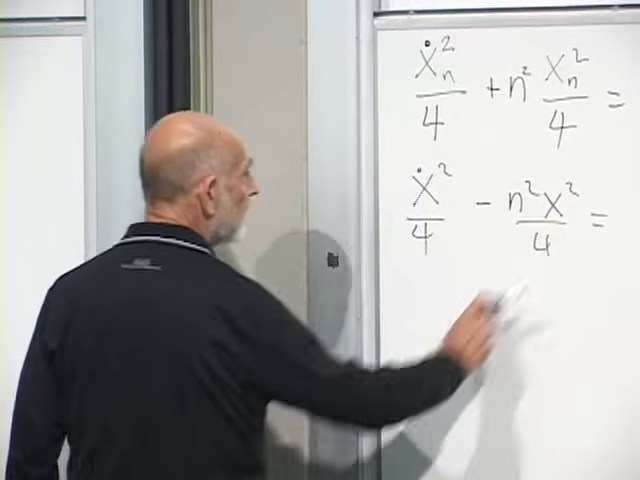
\includegraphics[width=0.82\textwidth]{lecture_03_figure_02.png}\caption{Phép tính trên bảng, trong đó giao hoán tử chính tắc cung cấp thừa số \(n\).}\lectureframe{00:10:30}\label{fig:l03-commutator-board}\end{figure}

Thừa số \(n\) chỉ ra cách chuẩn hóa các toán tử nâng hạ:

\begin{align}
  a_n
  &\equiv
  \frac{\sqrt n}{2}X_n+\frac{i}{\sqrt n}p_n,
  \label{eq:l03-annihilator}\\
  a_n^\dagger
  &\equiv
  \frac{\sqrt n}{2}X_n-\frac{i}{\sqrt n}p_n.
  \label{eq:l03-creator}
\end{align}

Chúng thỏa mãn

\begin{equation}
  [a_n,a_m^\dagger]=\delta_{nm},
  \qquad
  H_n=n\left(a_n^\dagger a_n+\frac12\right).
  \label{eq:l03-oscillator-algebra}
\end{equation}

Vì vậy, \(a_n^\dagger\) thêm một lượng tử vào dao động tử thứ \(n\), nhưng lượng tử đó mang \(n\) đơn vị năng lượng mode. Khoảng cách mức quen thuộc của dao động tử không hề mất đi; tần số của nó là \(\omega_n=n\).

\begin{figure}[H]\centering
  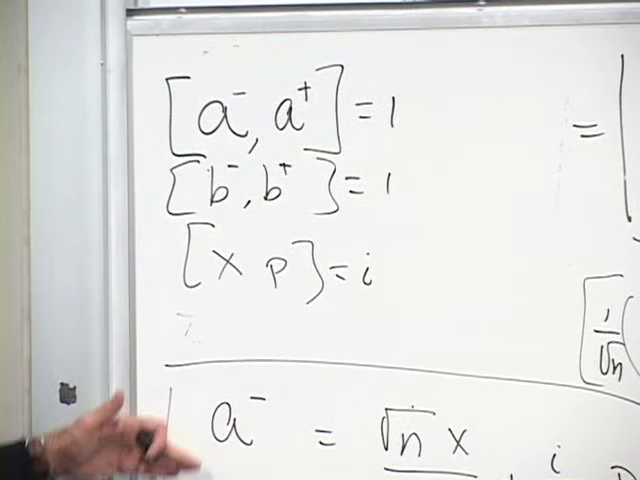
\includegraphics[width=0.82\textwidth]{lecture_03_figure_03.png}\caption{Các toán tử hủy và tạo đã được chuẩn hóa cho dao động tử dây thứ \(n\).}\lectureframe{00:12:00}\label{fig:l03-ladder-board}\end{figure}

\subsection{Hai tháp dao động ngang}

Trong không-thời gian 4 chiều, một dây mang động lượng rất lớn dọc theo trục \(z\) có hai tọa độ ngang, \(X\) và \(Y\). Vì vậy ta cần hai tháp dao động tử độc lập. Cho \(a_n,a_n^\dagger\) tác dụng lên các mode \(X\) và \(b_n,b_n^\dagger\) tác dụng lên các mode \(Y\). Giải \eqref{eq:l03-annihilator}--\eqref{eq:l03-creator} theo các tọa độ, ta được

\begin{equation}
  X_n=\frac{a_n+a_n^\dagger}{\sqrt n},
  \qquad
  Y_n=\frac{b_n+b_n^\dagger}{\sqrt n}.
  \label{eq:l03-mode-coordinates}
\end{equation}

\begin{figure}[H]\centering
  \includegraphics[width=0.78\textwidth]{lecture_03_figure_04.png}\caption{Biểu diễn một tọa độ mode theo các toán tử tạo và hủy của nó.}\lectureframe{00:17:05}\label{fig:l03-coordinate-operator-board}\end{figure}

Các tọa độ của dây mở được khai triển theo các mode Neumann,

\begin{align}
  X(\sigma,\tau)
  &=X_{\rm cm}(\tau)
    +\sum_{n=1}^{\infty}X_n(\tau)\cos(n\sigma),
  \label{eq:l03-X-fourier}\\
  Y(\sigma,\tau)
  &=Y_{\rm cm}(\tau)
    +\sum_{n=1}^{\infty}Y_n(\tau)\cos(n\sigma).
  \label{eq:l03-Y-fourier}
\end{align}

Các hàm cos xuất hiện vì độ dốc tại các đầu mút triệt tiêu. Thay \eqref{eq:l03-mode-coordinates} vào sẽ biến chính dây thành một toán tử:

\begin{align}
  X(\sigma,\tau)
  &=X_{\rm cm}(\tau)
    +\sum_{n=1}^{\infty}
      \frac{a_n(\tau)+a_n^\dagger(\tau)}{\sqrt n}
      \cos(n\sigma),
  \label{eq:l03-X-operator}\\
  Y(\sigma,\tau)
  &=Y_{\rm cm}(\tau)
    +\sum_{n=1}^{\infty}
      \frac{b_n(\tau)+b_n^\dagger(\tau)}{\sqrt n}
      \cos(n\sigma).
  \label{eq:l03-Y-operator}
\end{align}

\begin{figure}[H]\centering
  \begin{minipage}[t]{0.48\textwidth}\centering
    \includegraphics[width=\textwidth]{lecture_03_figure_05.png}\par\smallskip\footnotesize (a) Khai triển tọa độ theo mode.\end{minipage}\hfill
  \begin{minipage}[t]{0.48\textwidth}\centering
    \includegraphics[width=\textwidth]{lecture_03_figure_06.png}\par\smallskip\footnotesize (b) Các toán tử nâng hạ được thế vào các tọa độ dây.\end{minipage}\caption{Hình dạng của dây mở lượng tử được ghép lại từ tất cả các toán tử dao động ngang của nó.}\lectureframe{00:20:35 and 00:21:05}\label{fig:l03-string-coordinate-board}\end{figure}

\begin{classroomqa}\audiencequestion{Liệu \(X_n\) cũng là một hàm của \(\sigma\) không?\lecturetimestamp{00:21:48}}\lecturerresponse{Không. Sự phụ thuộc vào \(\sigma\) nằm hoàn toàn trong \(\cos(n\sigma)\). Hệ số \(X_n\) là biên độ phụ thuộc thời gian của mẫu không gian đó, nên \(X_n=X_n(\tau)\).}\end{classroomqa}

\begin{classroomqa}\audiencequestion{Vì sao các toán tử được gọi là nâng và hạ dường như lại có dấu ngược nhau?\lecturetimestamp{00:23:13}}\lecturerresponse{Dấu nhìn thấy được của \(ip_n\) không phải là quy tắc đặt tên. Hãy tính giao hoán tử với Hamiltonian. Toán tử thỏa mãn \([H_n,a_n^\dagger]=n a_n^\dagger\) làm tăng năng lượng; toán tử thỏa mãn \([H_n,a_n]=-n a_n\) làm giảm nó.}\end{classroomqa}

Bức tranh hai tháp ngang chỉ là một minh họa sư phạm trong 4 chiều. Một dây boson được lượng tử hóa nhất quán có 26 chiều không-thời gian, nên nó có 24 họ dao động tử ngang chứ không phải 2. Logic bên dưới không thay đổi: số trạng thái ở mức thứ nhất phải khớp với số phân cực vật lý của một vectơ không khối lượng trong cùng số chiều.

\section{Spin của hạt có khối lượng và helicity của hạt không khối lượng}

Trước khi gán spin cho các trạng thái dây, ta cần một sự phân biệt rành mạch. Một hạt có khối lượng với spin \(J\) có \(2J+1\) trạng thái spin,

\begin{equation}
  m_J=-J,-J+1,\ldots,J-1,J.
  \label{eq:l03-massive-spin-multiplet}
\end{equation}

Ví dụ, một hạt spin 1 có khối lượng có 3 phân cực và một hạt spin 2 có khối lượng có 5 phân cực. Ta có thể thấy vì sao bằng cách chuyển sang hệ quy chiếu nghỉ. Ở đó mọi phép quay không gian đều khả dụng. Xoay trục spin, boost trở lại, và mọi thành phần \(2J+1\) đều thuộc về cùng một hạt tương đối tính.

Một hạt không khối lượng không có hệ quy chiếu nghỉ. Nhãn spin bất biến của nó là helicity, tức mômen góc dọc theo hướng chuyển động. Photon chỉ có \(h=+1\) và \(h=-1\); graviton chỉ có \(h=+2\) và \(h=-2\). Một vô hướng có một trạng thái \(h=0\). Bài giảng dùng đối xứng phản xạ để ghép cặp hai helicity. Trong một lý thuyết chiral, một biểu diễn bất khả quy không khối lượng đơn lẻ có thể chỉ mang một helicity, nên việc ghép cặp là một phát biểu đối xứng bổ sung chứ không phải hệ quả chỉ riêng của tính không khối lượng.\editorialnote{Phân loại little group hiện đại cho phép các biểu diễn không khối lượng một-helicity. Tính chẵn lẻ hoặc một nội dung trường đầy đủ CPT thích hợp cung cấp helicity đối ngược trong các ví dụ photon và graviton quen thuộc.}

\begin{figure}[H]\centering
  \begin{minipage}[t]{0.45\textwidth}\centering
    \includegraphics[width=\textwidth]{lecture_03_figure_07.png}\par\smallskip\footnotesize (a) Phép đếm trạng thái spin được bắt đầu trên bảng.\end{minipage}\hfill
  \begin{minipage}[t]{0.5\textwidth}\centering
    \begin{adjustbox}{max width=\linewidth}\begin{tabular}{@{}ccc@{}}\toprule
      Spin &Trạng thái có khối lượng &Helicity không khối lượng \\\midrule
      \(0\) & \(1\) & \(0\) \\\(1\) & \(3\) & \(+1,-1\) \\\(2\) & \(5\) & \(+2,-2\) \\\bottomrule
    \end{tabular}\end{adjustbox}\end{minipage}\caption{Khối lượng tước đi hệ quy chiếu nghỉ và cùng với nó là các hình chiếu spin trung gian.}\lectureframe{00:27:40}\label{fig:l03-spin-count}\end{figure}

\subsection{Phân cực photon tuyến tính và tròn}

Xét một photon chuyển động dọc theo \(z\). Hai phân cực tuyến tính ngang của nó là \(\ket{x}\) và \(\ket{y}\). Chúng không phải là các trạng thái riêng helicity. Các trạng thái phân cực tròn là

\begin{align}
  \ket{R}
  &=\frac{1}{\sqrt2}\left(\ket{x}+i\ket{y}\right),
  \label{eq:l03-right-circular}\\
  \ket{L}
  &=\frac{1}{\sqrt2}\left(\ket{x}-i\ket{y}\right),
  \label{eq:l03-left-circular}
\end{align}

với helicity \(+1\) và \(-1\), tùy theo quy ước dùng để gọi phải và trái. Một photon phân cực tuyến tính là chồng chập của hai kết cục đó. Helicity trung bình của nó có thể triệt tiêu, nhưng một phép đo helicity không bao giờ tìm thấy một photon spin 0. Tương tự,

\begin{equation}
  \frac{1}{\sqrt2}\left(\ket{x}+\ket{y}\right)
\end{equation}

đơn giản là phân cực tuyến tính ở góc 45 độ.

\begin{figure}[H]\centering
  \begin{minipage}[t]{0.48\textwidth}\centering
    \includegraphics[width=\textwidth]{lecture_03_figure_08.png}\par\smallskip\footnotesize (a) Các trạng thái phân cực tròn trên bảng.\end{minipage}\hfill
  \begin{minipage}[t]{0.48\textwidth}\centering
    \begin{adjustbox}{max width=\linewidth}\begin{tikzpicture}[>=Latex,scale=0.9]
      \draw[->,thick] (0,0) -- (3.4,0) node[right] {\(z\)};
      \draw[->,blue!70!black,thick] (0,0) -- (0,2.0)
        node[above] {\(x\)};
      \draw[->,orange!85!black,thick] (0,0) -- (-1.4,-1.2)
        node[below left] {\(y\)};
      \draw[red!70!black,thick,->]
        plot[domain=0:320,samples=80]
        ({1.0*cos(\x)},{0.58*sin(\x)+0.4});
      \node[red!70!black] at (1.55,1.25) {circular};
    \end{tikzpicture}\end{adjustbox}\end{minipage}\caption{Phân cực tuyến tính cung cấp một cơ sở ngang; các tổ hợp tròn chéo hóa helicity.}\lectureframe{00:37:45}\label{fig:l03-polarization}\end{figure}

\begin{classroomqa}\audiencequestion{Điều này có giống sự tách các trạng thái spin trong thí nghiệm Stern--Gerlach không?\lecturetimestamp{00:37:40}}\lecturerresponse{Ý tưởng chồng chập lượng tử là như nhau, nhưng đối với photon thì ngôn ngữ trực tiếp là phân cực. Một phép đo phân cực tròn phân biệt hai helicity; không có photon dọc spin 0 nào trong chùm.}\end{classroomqa}

Graviton lặp lại mô thức đó ở spin 2. Để theo dõi spin, ta có thể viết một cách sơ đồ

\begin{equation}
  \ket{+2}\sim\ket{+1}\otimes\ket{+1},
  \qquad
  \ket{-2}\sim\ket{-1}\otimes\ket{-1}.
  \label{eq:l03-graviton-helicity}
\end{equation}

Điều này không có nghĩa là graviton theo nghĩa đen được tạo thành từ hai photon. Nó nói rằng hai helicity bằng nhau cộng lại cho helicity spin-2 đúng.

\begin{classroomqa}\audiencequestion{Phép tương tự hai photon có mở rộng sang các số lượng tử khác không?\lecturetimestamp{00:41:05}}\lecturerresponse{Không, nếu hiểu như một mô hình thành phần. Có những công thức mạnh, trong đó các biên độ hấp dẫn trông như tích, hay ``bình phương'', của các biên độ lý thuyết chuẩn, nhưng graviton vẫn là hạt riêng của nó. Phép tương tự đáng tin nhất ở đây là như một phát biểu về helicity.\editorialnote{Các quan hệ Kawai--Lewellen--Tye hiện đại và các quan hệ double-copy làm cho phát biểu về biên độ trở nên chính xác trong những lý thuyết thích hợp; chúng không biến graviton thành trạng thái liên kết của hai photon.}}\end{classroomqa}

\begin{classroomqa}\audiencequestion{Một photon có thể có bất kỳ động lượng nào, vậy chẳng phải nó có phổ liên tục thay vì phổ cô lập vốn được yêu cầu đối với một hạt sao?\lecturetimestamp{00:42:17}}\lecturerresponse{Biến liên tục là động lượng tâm khối. Giữ cố định động lượng đó và xét khối lượng bất biến nội tại. Một hạt được nhận diện bởi một mức khối lượng cô lập; rồi việc biến thiên động lượng toàn phần của nó tạo ra quan hệ tán sắc liên tục quen thuộc.}\end{classroomqa}

\enlargethispage{1pt}
\section{Các mức thấp nhất của dây mở}

Giờ ta có thể quay lại dây. Trong mô tả động lượng lớn, năng lượng light-front nội tại hữu hạn tỉ lệ với bình phương khối lượng bất biến. Tạm bỏ qua thang dây tổng thể, hãy viết phổ là

\begin{equation}
  \begin{aligned}
    M^2
    &=m_0^2
      +\sum_{n=1}^{\infty}n
       \left(N_n^{(a)}+N_n^{(b)}\right),\\
    N_n^{(a)}&=a_n^\dagger a_n,
    \qquad
    N_n^{(b)}=b_n^\dagger b_n.
  \end{aligned}
  \label{eq:l03-open-spectrum}
\end{equation}

Trạng thái cơ bản của các dao động tử thỏa mãn

\begin{equation}
  a_n\ket{0}=0,
  \qquad
  b_n\ket{0}=0,
  \qquad n=1,2,\ldots .
  \label{eq:l03-ground-annihilation}
\end{equation}

Đó không phải là sự vắng mặt trống rỗng của dây. Đó là dây lượng tử ít kích thích nhất, và các tọa độ của nó vẫn dao động. Gọi bình phương khối lượng của nó là \(m_0^2\), chưa được xác định.

\begin{figure}[H]\centering
  \includegraphics[width=0.78\textwidth]{lecture_03_figure_09.png}\caption{Trạng thái cơ bản của dây mở và các điều kiện hủy xác định nó.}\lectureframe{00:45:20}\label{fig:l03-ground-state-board}\end{figure}

Các kích thích ít tốn năng lượng nhất dùng các toán tử tạo \(n=1\):

\begin{equation}
  a_1^\dagger\ket{0},
  \qquad
  b_1^\dagger\ket{0},
  \qquad
  M^2=m_0^2+1.
  \label{eq:l03-first-level}
\end{equation}

\begin{figure}[H]\centering
  \includegraphics[width=0.78\textwidth]{lecture_03_figure_10.png}\caption{Một trong hai trạng thái bậc nhất suy biến, với phần tăng của bình phương khối lượng được viết trên bảng.}\lectureframe{00:49:25}\label{fig:l03-first-level-board}\end{figure}

Số ``một'' trong eqref{eq:l03-first-level} không phải là một joule, một electron volt hay một khối lượng Planck. Ta đã lược bỏ thang dây có thứ nguyên. Hiện thời, nó có nghĩa là một bậc trên thang bình phương khối lượng của dao động tử; các đơn vị còn thiếu sẽ được phục hồi trong bài giảng tiếp theo.

Mọi tổ hợp tuyến tính của hai trạng thái suy biến ấy cũng là một trạng thái ở mức này. Cụ thể,

\begin{equation}
  \frac{1}{\sqrt2}
  \left(a_1^\dagger\pm i b_1^\dagger\right)\ket{0}
  \label{eq:l03-string-circular-states}
\end{equation}

là phép tương tự trong dây của phân cực tròn. Dưới một phép quay trong mặt phẳng \(x\)-\(y\), \(a_1^\dagger\) và \(b_1^\dagger\) biến đổi như hai thành phần của một vectơ ngang. Vì thế các tổ hợp trong \eqref{eq:l03-string-circular-states} có helicity \(+1\) và \(-1\).

\begin{figure}[H]\centering
  \includegraphics[width=0.82\textwidth]{lecture_03_figure_11.png}\caption{Các điều kiện trạng thái cơ bản, hai kích thích bậc nhất và các tổ hợp tròn của chúng được tập hợp trên bảng.}\lectureframe{00:56:00}\label{fig:l03-level-structure-board}\end{figure}

Không có trạng thái suy biến thứ ba nào có thể đóng vai trò là một phân cực dọc. Nếu hai trạng thái này có khối lượng khác không, thì một hạt tương đối tính spin một sẽ cần ba phân cực. Với đúng hai phân cực, trạng thái đó phải không khối lượng. Do đó

\begin{equation}
  m_0^2+1=0,
  \qquad
  m_0^2=-1.
  \label{eq:l03-intercept-condition}
\end{equation}

Mức thứ nhất giống photon: đó là một trạng thái vectơ chuẩn không khối lượng. Nó không nhất thiết là photon của điện từ học; bản sắc chuẩn cuối cùng của nó phụ thuộc vào mô hình dây. Trạng thái cơ bản bên dưới nó có bình phương khối lượng âm. Đó là tachyon của dây mở boson.\editorialnote{Trong dây boson tới hạn đầy đủ, độ chặn do sắp thứ tự chuẩn và đại số Lorentz gắn với \(D=26\). Phép tính của bài giảng với hai hướng ngang là cái bóng 4 chiều của cùng một lập luận đếm trạng thái: \(D-2\) trạng thái dao động tử ở mức thứ nhất khớp với \(D-2\) phân cực vật lý của một vectơ không khối lượng.}

\begin{classroomqa}
\audiencequestion{Vì sao chúng ta phải quan tâm đến việc \(m_0^2\) âm?\lecturetimestamp{00:56:35}}
\lecturerresponse{Vì bình phương khối lượng là độ cong của thế trường bậc hai quanh trạng thái mà ta đã gọi là chân không. Độ cong âm có nghĩa là cấu hình này không phải là một trạng thái nền ổn định. Phép tính tiếp theo sẽ làm cho nhận định đó trở nên chính xác.}
\end{classroomqa}

\section{Tachyon thực sự có nghĩa là gì}

Tên gọi ``tachyon'' dễ gợi ra một suy nghĩ ban đầu gây hiểu lầm. Hãy bắt đầu từ hệ thức tán sắc tương đối tính với \(c=1\),

\begin{equation}
  E(p)=\sqrt{p^2+m^2}.
  \label{eq:l03-relativistic-dispersion}
\end{equation}

Đối với một gói sóng, vận tốc nhóm là

\begin{equation}
  v_g=\frac{dE}{dp}.
  \label{eq:l03-group-velocity}
\end{equation}

Điều này cho lại các trường hợp quen thuộc:

\begin{align}
  E_{\rm nr}(p)&=\frac{p^2}{2m},
  &v_g&=\frac{p}{m},
  \label{eq:l03-nr-group-velocity}\\
  E_\gamma(p)&=|p|,
  &|v_g|&=1,
  \label{eq:l03-photon-group-velocity}\\
  E_m(p)&=\sqrt{p^2+m^2},
  &|v_g|&=\frac{|p|}{\sqrt{p^2+m^2}}<1.
  \label{eq:l03-massive-group-velocity}
\end{align}

\begin{figure}[H]
  \centering
  \begin{minipage}[t]{0.48\textwidth}
    \centering
    \includegraphics[width=\textwidth]{lecture_03_figure_12.png}
    \par\smallskip\footnotesize (a) Vận tốc nhóm phi tương đối tính.
  \end{minipage}\hfill
  \begin{minipage}[t]{0.48\textwidth}
    \centering
    \includegraphics[width=\textwidth]{lecture_03_figure_13.png}
    \par\smallskip\footnotesize (b) Hệ thức tán sắc tương đối tính và đạo hàm của nó.
  \end{minipage}
  \caption{Đọc ra tốc độ lan truyền từ độ dốc của \(E(p)\).}
  \lectureframe{01:01:50 and 01:03:15}
  \label{fig:l03-group-velocity-board}
\end{figure}

Nếu \(m^2=-\mu^2\), thì biểu thức hình thức trở thành

\begin{equation}
  E(p)=\sqrt{p^2-\mu^2},
  \qquad
  v_g=\frac{p}{\sqrt{p^2-\mu^2}},
  \label{eq:l03-formal-tachyon-dispersion}
\end{equation}

biểu thức này có \(|v_g|>1\) bất cứ khi nào căn bậc hai là số thực. Nhưng đây không phải là cách diễn giải vật lý đúng của trạng thái cơ bản của dây boson. Rắc rối đã xuất hiện ngay ở xung lượng thấp, nơi tần số là ảo.

\subsection{Độ cong âm của thế trường}

Xét một trường vô hướng thực trong một chiều không gian,

\begin{equation}
  \left(\partial_t^2-\partial_x^2+m^2\right)\phi=0.
  \label{eq:l03-klein-gordon}
\end{equation}

Đối với một sóng phẳng \(\phi\propto e^{-i\omega t+ikx}\),

\begin{equation}
  \omega^2=k^2+m^2.
  \label{eq:l03-kg-dispersion}
\end{equation}

\begin{figure}[H]
  \centering
  \includegraphics[width=0.82\textwidth]{lecture_03_figure_14.png}
  \caption{Phương trình Klein--Gordon được dùng để làm lộ ra tính bất ổn định đằng sau bình phương khối lượng âm.}
  \lectureframe{01:06:40}
  \label{fig:l03-klein-gordon-board}
\end{figure}

Năng lượng bậc hai được bảo toàn là

\begin{equation}
  \mathcal E
  =\frac12\int dx\,
  \left[
    \dot\phi^{\,2}
    +(\partial_x\phi)^2
    +m^2\phi^2
  \right].
  \label{eq:l03-field-energy}
\end{equation}

\begin{figure}[H]
  \centering
  \includegraphics[width=0.82\textwidth]{lecture_03_figure_15.png}
  \caption{Năng lượng của trường vô hướng, trong đó hạng khối lượng cung cấp độ cong cục bộ của thế.}
  \lectureframe{01:08:10}
  \label{fig:l03-field-energy-board}
\end{figure}

Đối với \(m^2>0\), thế cục bộ
\(V(\phi)=\tfrac12m^2\phi^2\) có dạng một cái bát. Cấu hình \(\phi=0\) nằm ở đáy của nó. Đối với \(m^2=-\mu^2\), chính điểm ấy là đỉnh của một cái bát lật ngược.
Phương trình \eqref{eq:l03-kg-dispersion} trở thành

\begin{equation}
  \omega^2=k^2-\mu^2.
  \label{eq:l03-tachyonic-modes}
\end{equation}

Các mode với \(k^2<\mu^2\) có

\begin{equation}
  \omega=\pm i\sqrt{\mu^2-k^2},
  \qquad
  \phi_k(t)\propto
  e^{\pm\sqrt{\mu^2-k^2}\,t}.
  \label{eq:l03-growing-mode}
\end{equation}

Một nhánh tăng theo hàm mũ. Vì thế, trạng thái được coi là chân không là bất ổn định:
một nhiễu loạn bước sóng dài nhỏ tùy ý sẽ đẩy trường rời khỏi
\(\phi=0\). Đó là ý nghĩa của một tachyon trong phổ.

\subsection{Dãy con lắc dựng đứng}

Một hàng các con lắc ghép nối làm cho sự phân biệt này trở nên dễ thấy. Đặt mọi con lắc thẳng đứng. Cấu hình đồng nhất ấy tồn tại, nhưng nó cân bằng tại một cực đại của thế năng. Khẽ chạm một con lắc, nó sẽ đổ xuống, kéo theo các con lắc lân cận. Một mặt trước gồm các con lắc đang đổ lan dọc theo dãy với tốc độ tín hiệu hữu hạn do các liên kết ghép xác định.

\begin{figure}[H]
  \centering
  \begin{minipage}[t]{0.48\textwidth}
    \centering
    \includegraphics[width=\textwidth]{lecture_03_figure_16.png}
    \par\smallskip\footnotesize (a) Mô hình các con lắc dựng đứng ghép nối trên bảng.
  \end{minipage}\hfill
  \begin{minipage}[t]{0.48\textwidth}
    \centering
    \begin{adjustbox}{max width=\linewidth}
    \begin{tikzpicture}[>=Latex,scale=0.78]
      \draw[thick] (-0.3,0) -- (6.3,0);
      \foreach \x/\a in {0/0,1/0,2/8,3/28,4/55,5/72,6/78}{
        \fill (\x,0) circle (0.06);
        \draw[thick] (\x,0) -- ++({90-\a}:1.25);
        \fill[blue!65!black]
          ($(\x,0)+({90-\a}:1.25)$) circle (0.11);
      }
      \draw[red!70!black,->,thick] (1.7,-0.45) -- (4.6,-0.45)
        node[midway,below] {falling front};
    \end{tikzpicture}
    \end{adjustbox}
  \end{minipage}
  \caption{Tính bất ổn định lan truyền theo nhân quả qua một hệ dù phổ tuyến tính hóa của nó chứa bình phương khối lượng âm.}
  \lectureframe{01:10:40}
  \label{fig:l03-pendulum-instability}
\end{figure}

Không có gì trong cơ chế này cho phép một tín hiệu được điều khiển vượt lên trước mặt trước nhân quả. Một mode tachyonic chẩn đoán một điểm khai triển tồi, chứ không phải một sứ giả siêu quang ổn định.\editorialnote{Đối với một phương trình trường tương đối tính địa phương, vận tốc mặt trước vẫn là tốc độ nhân quả. Vận tốc nhóm hình thức của nhánh thực ở \(k\) lớn không biến chân không bất ổn định thành một kênh liên lạc nhanh hơn ánh sáng.}

\begin{classroomqa}
\audiencequestion{Trạng thái không khối lượng vừa tìm được có phải chính là graviton được lý thuyết dây dự đoán không?\lecturetimestamp{01:14:27}}
\lecturerresponse{Không. Đó là trạng thái spin một với hai phân cực của một dây mở, nên nó có tính chất giống boson chuẩn. Graviton là một kích thích spin hai của một dây kín.}
\end{classroomqa}

\begin{classroomqa}
\audiencequestion{Một thế lộn ngược có được phép về mặt toán học không, và sau khi rơi xuống thì hệ sẽ kết thúc ở đâu?\lecturetimestamp{01:15:17}}
\lecturerresponse{Nó hoàn toàn là một gần đúng cục bộ hợp lệ, nhưng tự bản thân nó không có trạng thái nền vì năng lượng không bị chặn dưới. Một thế đầy đủ hơn có thể lại uốn cong lên trên và có một cực tiểu thấp hơn. Khi đó hệ lăn xuống hoặc ngưng tụ về phía cấu hình ổn định ấy.}
\end{classroomqa}

Dây boson thông thường có đúng khuyết tật này. Các trạng thái dao động tử cao hơn của nó vẫn là một phần của phổ, nhưng chúng là các kích thích của một nền bất ổn định. Các lý thuyết siêu dây nhất quán loại bỏ tachyon của dây mở trong các sector ổn định của chúng, đồng thời vẫn giữ lại các kích thích dây không khối lượng và có khối lượng.

\begin{classroomqa}
\audiencequestion{Các tính chất khác của trạng thái dây mở ấy có phù hợp với photon tốt như hai phân cực của nó không?\lecturetimestamp{01:17:07}}
\lecturerresponse{Trạng thái đó ứng xử như một boson chuẩn không khối lượng. Các gán điện tích chi tiết, các quy tắc bức xạ và bản sắc của nó phụ thuộc vào mô hình dây, vì vậy nên gọi nó là giống photon hơn là lập tức đồng nhất nó với điện từ học. Những tính chất tương tác đó sẽ được phát triển ở phần sau.}
\end{classroomqa}

\section{Các dây tương tác như thế nào}

Phổ tự do chỉ là một nửa của lý thuyết. Các dây còn nhập lại và tách ra. Trước hết, hữu ích là nhớ rằng một dây tự do bị kích thích có thể mang mômen góc. Một dây thẳng đang quay quay quanh tâm khối của nó, và năng lượng cùng mômen góc của nó tăng cùng nhau dọc theo quỹ đạo kiểu dây quen thuộc.

\begin{figure}[H]
  \centering
  \includegraphics[width=0.72\textwidth]{lecture_03_figure_17.png}
  \caption{Phác họa một dây mở quay quanh điểm tâm khối của nó.}
  \lectureframe{01:19:30}
  \label{fig:l03-rotating-string-board}
\end{figure}

\begin{classroomqa}
\audiencequestion{Một dây tự do có thể quay lộn đầu quanh một đầu mút cố định không?\lecturetimestamp{01:20:02}}
\lecturerresponse{Không nếu không có chỗ neo. Một hệ tự do cô lập quay quanh tâm khối của nó. Nếu một đầu mút được gắn với một vật khác hoặc với một brane, thì hệ kết hợp có thể quay quanh một tâm khác, giống như electron và hạt nhân quay quanh tâm khối chung của chúng trong khi hạt nhân nặng hơn nhiều trông gần như cố định.}
\end{classroomqa}

\subsection{Đỉnh tương tác của dây mở}

Đối với dây mở, tương tác cơ bản xảy ra khi hai đầu mút gặp nhau tại cùng một điểm không-thời gian. Có một biên độ \(g_s\) để chúng nhập lại và tạo thành một dây. Đảo ngược diễn tiến đó cho một biên độ để một dây tách thành hai. Về sơ đồ,

\begin{equation}
  \text{open}+\text{open}
  \quad\rightleftarrows\quad
  \text{open}.
  \label{eq:l03-open-joining}
\end{equation}

\begin{figure}[H]
  \centering
  \begin{minipage}[t]{0.48\textwidth}
    \centering
    \includegraphics[width=\textwidth]{lecture_03_figure_18.png}
    \par\smallskip\footnotesize (a) Diễn tiến nhập lại trên bảng.
  \end{minipage}\hfill
  \begin{minipage}[t]{0.48\textwidth}
    \centering
    \begin{tikzpicture}[>=Latex,scale=0.9]
      \draw[->] (0,-2.1) -- (0,2.2) node[above] {time};
      \draw[blue!70!black,thick] (-2,-1.6) .. controls (-1.3,-0.9)
        and (-0.7,-0.35) .. (0,0);
      \draw[blue!70!black,thick] (2,-1.6) .. controls (1.3,-0.9)
        and (0.7,-0.35) .. (0,0);
      \draw[orange!85!black,thick] (0,0) .. controls (0.25,0.7)
        and (-0.15,1.25) .. (0.15,1.9);
      \fill[red!70!black] (0,0) circle (0.09);
      \node[right] at (0.12,0) {\(g_s\)};
    \end{tikzpicture}
  \end{minipage}
  \caption{Sự nhập của các đầu mút là phép tương tự trong lý thuyết dây của một đỉnh tương tác hạt địa phương; đảo ngược thời gian cho ra sự tách.}
  \lectureframe{01:24:05}
  \label{fig:l03-open-vertex}
\end{figure}

Hằng số ghép là một biên độ. Đối với một quá trình cơ bản đã chỉ định, xác suất tương ứng bắt đầu ở bậc \(|g_s|^2\), với các thừa số không gian pha và chuẩn hóa do phép tính đầy đủ cung cấp. Vì vậy, gọi \(g_s\) là ``xác suất'' chỉ là một lối nói tắt không chính thức; việc giữ biên độ và xác suất phân biệt nhau sẽ tránh được một bình phương giả tạo.

Tương tác không phụ thuộc vào việc dây ngoài đang dao động, đang quay hay ở một trạng thái dao động tử nào khác. Những trạng thái ấy làm thay đổi phần tử ma trận chi tiết, nhưng cùng một quy tắc nhập cục bộ vẫn được dùng.

\subsection{Một dây mở có thể tự khép lại}

Giả sử hai đầu mút của một dây mở gặp nhau. Quy tắc nhập không thể biết rằng chúng thuộc cùng một dây. Chúng có thể hợp nhất, tạo ra một vòng kín:

\begin{equation}
  \text{open}\longrightarrow\text{closed}.
  \label{eq:l03-self-closing}
\end{equation}

\begin{figure}[H]
  \centering
  \begin{minipage}[t]{0.48\textwidth}
    \centering
    \includegraphics[width=\textwidth]{lecture_03_figure_19.png}
    \par\smallskip\footnotesize (a) Dây mở đưa hai đầu mút của nó lại với nhau.
  \end{minipage}\hfill
  \begin{minipage}[t]{0.48\textwidth}
    \centering
    \begin{tikzpicture}[>=Latex,scale=0.92]
      \draw[blue!70!black,thick]
        (-2,0) .. controls (-1.2,1.5) and (1.2,1.5) .. (2,0);
      \fill[red!70!black] (-2,0) circle (0.08);
      \fill[red!70!black] (2,0) circle (0.08);
      \draw[->,thick] (-0.45,-0.45) -- (0.45,-0.45);
      \draw[orange!85!black,thick] (0,-1.55) ellipse (1.15 and 0.58);
      \node at (0,-2.25) {closed string};
    \end{tikzpicture}
  \end{minipage}
  \caption{Các dây mở tương tác tất yếu sinh ra các dây kín.}
  \lectureframe{01:27:20}
  \label{fig:l03-open-becomes-closed}
\end{figure}

Đây không phải là một sự tô điểm tùy chọn. Bất kỳ lý thuyết nào về các dây mở tương tác đều phải chứa các trạng thái dây kín. Quá trình ngược lại cho phép một dây kín mở thành một dây mở khi có mặt các đầu mút được phép và các điều kiện biên.

\begin{classroomqa}
\audiencequestion{Khi các dây hợp nhất hoặc tách ra, năng lượng dao động tử của chúng có thay đổi không, và lý thuyết có xác định cách thay đổi ấy không?\lecturetimestamp{01:28:05}}
\lecturerresponse{Có. Năng lượng và động lượng được bảo toàn cho toàn bộ quá trình, còn sự kích thích có thể được phân bố lại giữa các dây đi ra. Đỉnh tương tác và các hàm sóng ngoài xác định biên độ chuyển tiếp.}
\end{classroomqa}

\subsection{Các dây kín có thể tương tác mà không cần mở ra}

Hệ quả này chỉ theo một chiều. Các dây mở tương tác đòi hỏi phải có dây kín, nhưng một lý thuyết có thể bắt đầu chỉ với các dây kín. Hai vòng kín có thể chạm nhau, nối lại và trở thành một vòng kín; lịch sử đảo ngược tách một vòng thành hai. Không cần xuất hiện đầu mút mở nào.

\begin{figure}[H]
  \centering
  \begin{minipage}[t]{0.48\textwidth}
    \centering
    \includegraphics[width=\textwidth]{lecture_03_figure_20.png}
    \par\smallskip\footnotesize (a) Sự hợp nhất của dây kín trên bảng.
  \end{minipage}\hfill
  \begin{minipage}[t]{0.48\textwidth}
    \centering
    \begin{tikzpicture}[>=Latex,scale=0.88]
      \draw[blue!70!black,thick] (-1.35,0) circle (0.75);
      \draw[blue!70!black,thick] (1.35,0) circle (0.75);
      \draw[->,thick] (-0.35,-1.15) -- (0.35,-1.15);
      \draw[orange!85!black,thick] (0,-2.3) ellipse (1.35 and 0.68);
      \node at (0,1.2) {closed \(+\) closed};
      \node at (0,-3.25) {closed};
    \end{tikzpicture}
  \end{minipage}
  \caption{Các dây kín có tương tác nhập và tách riêng của chúng và không cần đi qua một trạng thái dây mở.}
  \lectureframe{01:29:05}
  \label{fig:l03-closed-fusion}
\end{figure}

\begin{classroomqa}
\audiencequestion{Nếu một lý thuyết bắt đầu với các dây kín, liệu nó cũng phải chứa các dây mở không?\lecturetimestamp{01:28:35}}
\lecturerresponse{Không. Các dây kín có thể tương tác bằng cách nối lại trong khi vẫn kín suốt quá trình. Các dây mở đòi hỏi dữ liệu biên bổ sung, chẳng hạn như các đầu mút được phép hoặc các brane.}
\end{classroomqa}

\section{Vì sao không thể tránh được hấp dẫn}

Phép tính dao động tử của dây kín song song với phép tính của dây mở, nhưng có các kích thích truyền trái và truyền phải độc lập. Mức khớp thấp nhất không tầm thường của chúng chứa một trạng thái spin hai không khối lượng. Trạng thái đó có các độ xoắn của một graviton. Hệ quả là mọi lý thuyết dây kín tương tác nhất quán đều chứa hấp dẫn.

\begin{classroomqa}
\audiencequestion{Vì sao kích thích dây kín thấp nhất lại phải là một graviton, đúng như mức dây mở đã buộc phải giống photon?
\lecturetimestamp{01:30:59}}
\lecturerresponse{Câu trả lời là cùng một kiểu đếm trạng thái, giờ đây với các vectơ dao động tử truyền trái và truyền phải. Tích tensor của chúng chứa một phân cực spin hai đối xứng không vết không khối lượng. Phổ dây kín tường minh sẽ được tính ra tiếp theo; ở giai đoạn này, điều cốt yếu là tính tất yếu của trạng thái đó.}
\end{classroomqa}

Các dây mở và dây kín cũng có thể tương tác với nhau. Một vòng kín có thể gặp một dây mở và bị hấp thụ, để lại một dây mở lớn hơn hoặc bị kích thích theo cách khác. Ngược lại, một dây mở có thể bức xạ ra một vòng kín. Ở mức hạt, đây là sự phát xạ hoặc hấp thụ một graviton bởi vật chất.

\begin{figure}[H]
  \centering
  \begin{minipage}[t]{0.48\textwidth}
    \centering
    \includegraphics[width=\textwidth]{lecture_03_figure_21.png}
    \par\smallskip\footnotesize (a) Sự nối lại cục bộ của các đoạn dây.
  \end{minipage}\hfill
  \begin{minipage}[t]{0.48\textwidth}
    \centering
    \includegraphics[width=\textwidth]{lecture_03_figure_22.png}
    \par\smallskip\footnotesize (b) Một vòng kín gắn vào một dây mở.
  \end{minipage}
  \caption{Các hình vẽ trên bảng minh họa các tương tác hỗn hợp dây mở--dây kín và khả năng phổ quát của sự trao đổi graviton.}
  \lectureframe{01:33:10 and 01:34:35}
  \label{fig:l03-mixed-interactions-board}
\end{figure}

\begin{figure}[H]
  \centering
  \begin{tikzpicture}[>=Latex,scale=0.88]
    \draw[blue!70!black,thick]
      (-3,-0.5) .. controls (-1.7,-0.1) and (-0.8,0.2) .. (0,0);
    \draw[blue!70!black,thick]
      (0,0) .. controls (0.9,0.3) and (2.0,0.1) .. (3,0.55);
    \draw[orange!85!black,thick] (-0.8,1.55) ellipse (0.75 and 0.45);
    \draw[->,red!70!black,thick] (-0.45,1.15) -- (-0.05,0.35);
    \node[blue!70!black] at (-2.2,-0.95) {open string};
    \node[orange!85!black] at (-0.8,2.25) {closed string};
    \node at (1.75,-0.5) {excited open string};
  \end{tikzpicture}
  \caption{Một sơ đồ gọn gàng, không gắn với không-thời gian, của sự hấp thụ một dây kín bởi một dây mở.}
  \label{fig:l03-mixed-interaction-redraw}
\end{figure}

Graviton có thể ghép với mọi trạng thái dây vì mọi dây đều mang năng lượng và động lượng, và các quy tắc nhập cho phép trao đổi dây kín. Đây là nguồn gốc trong lý thuyết dây của tính phổ quát của hấp dẫn.

\begin{classroomqa}
\audiencequestion{Liệu một dây kín có thể trở thành một dây mở, hoặc nó có thể nhập với một dây mở mà không vi phạm quy tắc đầu mút không?\lecturetimestamp{01:31:20}}
\lecturerresponse{Trong một lý thuyết chứa cả hai sector, một dây kín có thể gắn vào một dây mở và làm thay đổi trạng thái của nó. Việc một dây kín đơn lẻ có thể đơn giản mở ra hay không phụ thuộc vào việc lý thuyết có cung cấp các đầu mút được phép hay không. Quy tắc nối lại cục bộ vẫn giữ nguyên.}
\end{classroomqa}

\begin{classroomqa}
\audiencequestion{Các vòng kín có thể trở nên móc nối với nhau hoặc bị thắt nút vĩnh viễn không?\lecturetimestamp{01:35:10}}
\lecturerresponse{Ở ghép yếu, các dây hầu như trong suốt đối với nhau: chúng có thể xuyên qua nhau trừ khi biên độ tái nối nhỏ đó phát huy tác dụng. Vì thế, một sự móc nối hay thắt nút có thể tồn tại một thời gian, nhưng tôpô có thể thay đổi khi xảy ra một tương tác dây được phép.}
\end{classroomqa}

\begin{classroomqa}
\audiencequestion{Xác suất tương tác có độc lập với trạng thái hay tốc độ của dây không?\lecturetimestamp{01:36:09}}
\lecturerresponse{Sự ghép cục bộ được đặc trưng bởi cùng một tham số, nhưng xác suất chuyển tiếp toàn phần còn phụ thuộc vào các hàm sóng và vào việc những phần liên quan còn tiếp xúc với nhau trong bao lâu. Một lần gặp nhanh nhìn chung cho ít thời gian tương tác hơn một lần gặp chậm.}
\end{classroomqa}

\section{Thang độ và hằng số ghép còn thiếu}

Hai chi tiết kỹ thuật đã được cố ý hoãn lại. Thứ nhất, \(X\) là một độ dài còn \(a_n\) là không thứ nguyên, nên quan hệ tỉ lệ trong \eqref{eq:l03-mode-coordinates} phải chứa một thang độ độ dài. Thứ hai, việc nâng mức dao động tử không thể theo nghĩa đen cộng một số không thứ nguyên vào một bình phương khối lượng vật lý. Khôi phục độ dài dây \(\ell_s\), hoặc tương đương là độ dốc Regge \(\alpha'\sim\ell_s^2\), sẽ cung cấp các thứ nguyên còn thiếu:

\begin{equation}
  M^2\sim\frac{1}{\alpha'}(N-a).
  \label{eq:l03-dimensional-spectrum}
\end{equation}

Quy ước và chuẩn hóa chính xác sẽ được ấn định trong bài giảng tiếp theo.

\begin{classroomqa}
\audiencequestion{Điều gì ấn định đơn vị độ dài của dây và lượng khối lượng do một toán tử tạo thêm vào?\lecturetimestamp{01:37:03}}
\lecturerresponse{Một hằng số có thứ nguyên đã bị lược bỏ. Đó là thang độ của dây, thường được viết là \(\ell_s\) hoặc \(\alpha'\). Các toán tử dao động tử là không thứ nguyên; các lũy thừa của thang độ đó biến số mức của chúng thành độ dài, sức căng và bình phương khối lượng vật lý.}
\end{classroomqa}

Tham số thứ hai là hằng số ghép dây \(g_s\). Trong cách trình bày đơn giản nhất, nó là một con số phổ quát chi phối sự nối và tách. Trong các mô hình phong phú hơn, các đầu mút có thể mang những nhãn khác nhau và các dây có thể gặp nhau tại các nút nối. Một cấu hình hình chữ Y là dạng tương tự trong lý thuyết dây của việc ba ống thông lượng gặp nhau; trong bức tranh hadron cũ, nó gắn với một baryon ba quark, còn một đoạn hở đơn lẻ thì giống một meson quark--phản quark.

\begin{classroomqa}
\audiencequestion{Các đầu mút dây khác nhau có thể có xác suất nối khác nhau không?\lecturetimestamp{01:39:31}}
\lecturerresponse{Mô hình đơn giản nhất dùng một hằng số ghép. Các lý thuyết công phu hơn gán điện tích hoặc nhãn biên cho các đầu mút, và khi đó các quy tắc chọn quyết định những sự nối nào được phép. Cách xây dựng chi tiết được để lại sau, nhưng ý tưởng về sự nối cục bộ phổ quát vẫn còn nguyên.}
\end{classroomqa}

\begin{classroomqa}
\audiencequestion{Một dây có thể tách dọc theo chiều dài của nó hoặc tạo thành một nút nối hình chữ Y không?\lecturetimestamp{01:40:01}}
\lecturerresponse{Một số hệ dây quả thật cho phép các nút nối. Chúng không phải là quá trình tách thông thường với hai đầu mút vừa được vẽ, nhưng chúng xuất hiện khi lý thuyết có các điện tích dây tương thích. Phép tương tự ống thông lượng meson--baryon là một hình ảnh hữu ích cho sự phân biệt này.}
\end{classroomqa}

\begin{classroomqa}
\audiencequestion{Việc thay đổi số chiều không-thời gian có làm thay đổi hằng số ghép tương tác không?\lecturetimestamp{01:42:25}}
\lecturerresponse{Số chiều làm thay đổi phổ, không gian pha và các hằng số ghép hiệu dụng thu được sau khi compact hóa. Hằng số ghép dây cơ bản vẫn tổ chức khai triển nhiễu loạn, nhưng dạng xuất hiện của nó ở số chiều thấp hơn phụ thuộc vào hình học và thể tích của các chiều phụ thêm.}
\end{classroomqa}

\begin{classroomqa}
\audiencequestion{Có phải chính hấp dẫn làm cho một dây tự do chuyển động ngay từ đầu không?\lecturetimestamp{01:43:17}}
\lecturerresponse{Không cần lực nào để duy trì chuyển động. Vị trí và vận tốc ban đầu xác định một nghiệm tự do; quán tính mang nó tiến về phía trước. Hấp dẫn hoặc một lực khác làm thay đổi chuyển động ấy. Hỏi điều gì đã gây ra các điều kiện ban đầu là một câu hỏi riêng, không phải là một phần của phương trình chuyển động cục bộ.}
\end{classroomqa}

Vì vậy, chúng ta đã đi tới ba kết luận liên hệ với nhau. Việc lượng tử hóa một dây hở tạo ra một vectơ không khối lượng ở mức kích thích thứ nhất của nó; trạng thái cơ sở boson nằm dưới mức đó là không ổn định; và các tương tác tất yếu đưa vào các dây kín, mà phổ của chúng chứa hấp dẫn. Nhiệm vụ tiếp theo là khôi phục thang độ còn thiếu và thực hiện tường minh việc lượng tử hóa dây kín.
\chapter{Chuỗi kín, sự khớp mức và đối ngẫu}

\lectureoverview{Một chuỗi kín mang các sóng độc lập theo hai hướng nội tại của nó. Việc lượng tử hóa các sóng ấy thoạt đầu dường như nhân đôi photon của chuỗi mở, nhưng tính bất biến dưới phép dời gốc của tọa độ chuỗi loại bỏ các trạng thái một phía. Mức đầu tiên còn lại chứa một hạt không khối lượng spin hai. Cũng chính ý tưởng đổi cách mô tả ấy mở ra một câu hỏi rộng hơn: khi các độ ghép thay đổi, nói rằng một đối tượng là cơ bản rốt cuộc có nghĩa gì?}

\section{Một bộ sinh để dành}

Trước khi vẽ một chuỗi kín, ta hãy nhắc lại một dữ kiện từ cơ học chính tắc. Giả sử
\begin{equation}
  L=L(q_i,\dot q_i),
\end{equation}
và định nghĩa động lượng liên hợp với \(q_i\) bởi
\begin{equation}
  p_i=\frac{\partial L}{\partial\dot q_i}.
\end{equation}
Một phép biến đổi liên tục vô cùng bé có thể được viết thành
\begin{equation}
  \delta q_i=\epsilon f_i(q),
  \label{eq:l04-infinitesimal-transformation}
\end{equation}
trong đó \(\epsilon\) là một tham số nhỏ. Nếu phép biến đổi này là một đối xứng, định lý Noether cho ta một điện tích bảo toàn. Chia độ dời tọa độ cho tham số chung ấy, ta được bộ sinh
\begin{equation}
  Q=\sum_i p_i f_i(q)
   =\frac{1}{\epsilon}\sum_i p_i\,\delta q_i.
  \label{eq:l04-noether-charge}
\end{equation}
Trong cơ học lượng tử, \(Q\) là toán tử sinh ra phép biến đổi vô cùng bé tương ứng.

Phép quay trong mặt phẳng \(xy\) là ví dụ quen thuộc. Với một lựa chọn định hướng,
\begin{equation}
  \delta x=\epsilon y,
  \qquad
  \delta y=-\epsilon x,
\end{equation}
và \eqref{eq:l04-noether-charge} trở thành mômen động lượng, với cùng lựa chọn dấu đó. Ví dụ cụ thể không quan trọng. Điều quan trọng là khuôn mẫu: động lượng co với độ dời vô cùng bé cho ta bộ sinh.

\begin{figure}[H]
  \centering
  \includegraphics[width=0.76\textwidth]{lecture_04_figure_01.png}
  \caption{Động lượng chính tắc và bộ sinh Noether được giữ lại để dùng cho phép dời sau này của tọa độ chuỗi kín.}
  \lectureframe{00:05:00}
  \label{fig:l04-noether-board}
\end{figure}

Chúng ta sẽ sớm gặp một đối xứng mà tọa độ của nó không phải là một điểm trong không gian thông thường mà là cách gán nhãn các điểm dọc theo một chuỗi. Phương trình \eqref{eq:l04-noether-charge} được nhắc lại ở đây nhằm phục vụ mục đích đó.

\section{Một tọa độ quanh một vòng kín}

Một chuỗi kín không có đầu mút. Chọn một tham số
\begin{equation}
  0\leq \sigma<2\pi
\end{equation}
và, tạm thời, đánh dấu một điểm là \(\sigma=0\). Đi nửa vòng là
\(\sigma=\pi\); đi một phần tư vòng và ba phần tư vòng lần lượt là \(\pi/2\) và
\(3\pi/2\). Dấu mốc này xác lập một quy ước tọa độ, chứ chưa phải một đặc trưng vật lý.

\begin{figure}[H]
  \centering
  \begin{minipage}[t]{0.58\textwidth}
    \centering
    \includegraphics[width=\textwidth]{lecture_04_figure_02.png}
    \par\smallskip\footnotesize (a) Vòng kín được đánh dấu trên bảng.
  \end{minipage}\hfill
  \begin{minipage}[t]{0.37\textwidth}
    \centering
    \begin{adjustbox}{max width=\linewidth}
    \begin{tikzpicture}[scale=0.82]
      \draw[thick]
        (0.1,1.1)
        .. controls (1.0,1.55) and (2.4,1.45) .. (2.9,0.4)
        .. controls (3.25,-0.45) and (2.45,-1.35) .. (1.55,-1.05)
        .. controls (0.65,-1.45) and (-0.35,-1.0) .. (-0.35,-0.05)
        .. controls (-0.35,0.55) and (-0.05,0.9) .. (0.1,1.1);
      \fill (0.1,1.1) circle (1.8pt);
      \node[above] at (0.1,1.12) {\(\sigma=0\)};
      \draw[->,thick] (2.55,0.95) arc[start angle=42,end angle=-25,radius=0.62];
      \node[right] at (3.05,0.55) {increasing \(\sigma\)};
    \end{tikzpicture}
    \end{adjustbox}
    \par\smallskip\footnotesize (b) Định hướng nội tại.
  \end{minipage}
  \caption{Một điểm được đánh dấu để xác định gốc, và một mũi tên cố định chiều mà \(\sigma\) tăng.}
  \lectureframe{00:06:48}
  \label{fig:l04-closed-string-origin}
\end{figure}

Mũi tên dọc theo vòng là một định hướng \emph{nội tại}. Không được nhầm nó với chuyển động theo chiều kim đồng hồ hay ngược chiều kim đồng hồ trong mặt phẳng \(xy\). Hãy hình dung một dây thun có đánh dấu được nhấc khỏi bảng, lật mặt, rồi đặt lại. Chiều kim đồng hồ biểu kiến của nó bị đảo ngược, còn thứ tự các dấu nội tại của nó thì không. Chiều tăng của \(\sigma\) vẫn là chiều tăng của \(\sigma\).

Sự phân biệt này chi phối cách dùng các thuật ngữ sóng truyền sang phải và sóng truyền sang trái. Trong chương này, một nhiễu loạn truyền sang phải có nghĩa là nó truyền theo chiều \(\sigma\) tăng, còn một nhiễu loạn truyền sang trái có nghĩa là nó truyền theo chiều \(\sigma\) giảm. Không tên gọi nào trong hai tên đó cho biết nhiễu loạn trông như chuyển động theo hướng nào trong căn phòng.

Định hướng từng giữ một vai trò cụ thể trong bức tranh chuỗi hadron ban đầu. Khi một ống thông lượng có định hướng bị bẻ gãy, một quark xuất hiện ở một đầu mút và một phản quark ở đầu kia; mũi tên nội tại phân biệt hai đầu. Cũng có thể xây dựng các lý thuyết chuỗi không định hướng, nhưng trong thảo luận hiện tại ta giữ lại mũi tên ấy cùng hai chiều dọc theo nó.

\section{Tính tuần hoàn và sóng chạy}

Gọi \(X(\sigma,\tau)\) và \(Y(\sigma,\tau)\) là hai tọa độ ngang của
chuỗi, với \(\tau\) ký hiệu thời gian. Các tọa độ ngang bổ sung, khi
có, được xử lý hoàn toàn theo cùng cách. Vì \(\sigma=0\) và
\(\sigma=2\pi\) gán nhãn cùng một điểm,
\begin{equation}
  X(\sigma+2\pi,\tau)=X(\sigma,\tau),
  \qquad
  Y(\sigma+2\pi,\tau)=Y(\sigma,\tau).
  \label{eq:l04-periodicity}
\end{equation}

\begin{figure}[H]
  \centering
  \includegraphics[width=0.76\textwidth]{lecture_04_figure_03.png}
  \caption{Điều kiện biên tuần hoàn cho hai tọa độ ngang.}
  \lectureframe{00:12:40}
  \label{fig:l04-periodicity-board}
\end{figure}

Vì vậy, một gợn cục bộ có thể tuần hoàn mãi mãi. Khi nó tới
\(2\pi\), nó đơn giản xuất hiện lại tại \(0\). Điều này khác với chuỗi mở,
ở đó một sóng chạy đi tới một đầu mút rồi phản xạ; cái đang truyền sang trái
trở thành truyền sang phải và ngược lại. Sóng dừng là tự nhiên cho chuỗi mở,
trong khi chuỗi kín cho phép hai họ lan truyền độc lập.

\subsection{Các mode Fourier phức}

Cơ sở thuận tiện cho một hàm tuần hoàn là
\begin{equation}
  e^{in\sigma}=\cos(n\sigma)+i\sin(n\sigma),
  \qquad n\in\mathbb Z.
\end{equation}
Điều kiện nguyên bị tính tuần hoàn ép buộc:
\(e^{in(\sigma+2\pi)}=e^{in\sigma}\). Chẳng hạn, thay \(n\) bằng một bán nguyên sẽ làm hàm thay đổi sau một vòng.

Tạm thời bỏ qua phụ thuộc theo thời gian, khai triển trên bảng là
\begin{align}
  X(\sigma)
  &=
  X_0+
  \sum_{n>0}X_n e^{in\sigma}
  +\sum_{n>0}X_{-n}e^{-in\sigma},
  \label{eq:l04-fourier-x}\\
  Y(\sigma)
  &=
  Y_0+
  \sum_{n>0}Y_n e^{in\sigma}
  +\sum_{n>0}Y_{-n}e^{-in\sigma}.
  \label{eq:l04-fourier-y}
\end{align}
Với \(X\) và \(Y\) thực, các hệ số chỉ số âm là liên hợp phức của các hệ số chỉ số dương ở mức cổ điển. Các mode không \(X_0\) và \(Y_0\) xác định tâm khối; chúng là vị trí, không phải các dao động nội tại.

\begin{figure}[H]
  \centering
  \includegraphics[width=0.82\textwidth]{lecture_04_figure_04.png}
  \caption{Các phần chỉ số dương và âm của khai triển Fourier tuần hoàn, tiếp theo là mode không.}
  \lectureframe{00:20:00}
  \label{fig:l04-fourier-board}
\end{figure}

\begin{classroomqa}
\audiencequestion{Nếu đây là các sóng chuyển động, thì tọa độ thời gian ở đâu?\lecturetimestamp{00:19:05}}
\lecturerresponse{Nó chỉ bị lược đi trong ký hiệu trên bảng. Một nghiệm truyền mang một pha phụ thuộc cả \(\sigma\) lẫn \(\tau\). Với quy ước dùng bên dưới, một họ có
\(e^{-in(\tau-\sigma)}\) và họ kia có
\(e^{-in(\tau+\sigma)}\).}
\end{classroomqa}

Vì vậy, chính toàn bộ pha, chứ không phải riêng dấu của \(n\) trong một thừa số Fourier thuần không gian tự nó, mới quyết định sự lan truyền. Ta có thể viết
\begin{equation}
  X(\sigma,\tau)=X_R(\tau-\sigma)+X_L(\tau+\sigma),
  \label{eq:l04-chiral-solution}
\end{equation}
và tương tự cho \(Y\). Họ nào được gọi là \(R\) chứ không phải \(L\) là một quy ước; sự kiện bất biến là có hai chiều ngược nhau dọc theo vòng tròn \(\sigma\).\editorialnote{Một thừa số \(e^{in\sigma}\) tại một thời điểm tự nó không xác định một sóng chuyển động. Sự lan truyền chỉ được cố định sau khi đã bổ sung pha thời gian.}

\section{Năng lượng theo hai chiều}

Động lực học cục bộ giống hệt như đối với dây mở. Trong chuẩn hóa đơn giản hóa dùng ở đây,
\begin{equation}
  L\propto
  \int_0^{2\pi}d\sigma\,
  \left[
    \dot X^2-X'^2+\dot Y^2-Y'^2
  \right],
  \label{eq:l04-string-lagrangian}
\end{equation}
trong đó dấu chấm ký hiệu \(\partial_\tau\) và dấu nháy ký hiệu
\(\partial_\sigma\). Năng lượng có dấu cộng giữa hạng động năng và hạng đàn hồi:
\begin{equation}
  E\propto
  \int_0^{2\pi}d\sigma\,
  \left[
    \dot X^2+X'^2+\dot Y^2+Y'^2
  \right].
  \label{eq:l04-string-energy}
\end{equation}
Đối với mỗi tọa độ ngang,
\begin{equation}
  \dot X^2+X'^2
  =
  \frac12(\dot X+X')^2+
  \frac12(\dot X-X')^2.
  \label{eq:l04-energy-square-completion}
\end{equation}
Các hạng chéo triệt tiêu, để lại chính xác các hạng động năng và gradient ban đầu.

\begin{figure}[H]
  \centering
  \includegraphics[width=0.82\textwidth]{lecture_04_figure_05.png}
  \caption{Tổng năng lượng được sắp xếp lại thành hai sector sóng chạy.}
  \lectureframe{00:25:10}
  \label{fig:l04-energy-board}
\end{figure}

Với \(X_R(\tau-\sigma)\), ta có \(\dot X_R=-X_R'\); còn với
\(X_L(\tau+\sigma)\), ta có \(\dot X_L=X_L'\). Do đó, hai bình phương trong \eqref{eq:l04-energy-square-completion} tách riêng hai họ chiral. Gộp mọi tọa độ ngang lại, ta định nghĩa
\begin{align}
  E_L&\propto
  \frac12\int_0^{2\pi}d\sigma
  \sum_I(\dot X^I+X^{I\prime})^2,\\
  E_R&\propto
  \frac12\int_0^{2\pi}d\sigma
  \sum_I(\dot X^I-X^{I\prime})^2.
  \label{eq:l04-left-right-energies}
\end{align}
Khi đó \(E=E_L+E_R\). Vì các phương trình ở giai đoạn này là tuyến tính, các sóng từ hai sector đi xuyên qua nhau mà không tán xạ.

\subsection{Số dao động tử gấp đôi}

Thay chuỗi Fourier vào
\eqref{eq:l04-string-lagrangian} sẽ biến mỗi hệ số mode khác không thành một dao động tử điều hòa. Tần số của nó tỉ lệ với \(|n|\): bước sóng ngắn hơn có nghĩa là tần số cao hơn và do đó năng lượng kích thích lớn hơn. Khác với dây mở, mỗi tần số dương xuất hiện trong hai bản sao lan truyền độc lập.

Trên bảng, các toán tử tạo phân cực theo \(X\) được ký hiệu là
\(a_n^+\) và \(a_{-n}^+\), còn các toán tử phân cực theo \(Y\) là
\(b_n^+\) và \(b_{-n}^+\). Để tách biệt rõ hơn giữa toán tử tạo và hướng lan truyền, ta sẽ viết
\begin{equation}
  a_n^\dagger,\quad b_n^\dagger,
  \qquad
  \widetilde a_n^\dagger,\quad\widetilde b_n^\dagger,
  \qquad n>0.
  \label{eq:l04-oscillator-notation}
\end{equation}
Các toán tử không ngã và có ngã tạo ra các hướng đối nhau trên mặt thế giới; \(a\) và \(b\) ký hiệu hai phân cực ngang.

\begin{figure}[H]
  \centering
  \includegraphics[width=0.65\textwidth]{lecture_04_figure_06.png}
  \caption{Ký hiệu trên bảng cho các toán tử tạo phân cực theo \(X\) và \(Y\) đã được nhân đôi.}
  \lectureframe{00:29:10}
  \label{fig:l04-oscillators-board}
\end{figure}

Nếu \(N_n^{(a)},N_n^{(b)}\) và các đối tác có ngã của chúng là các số chiếm, thì các mức dao động tử do hai chiều mang được cho một cách sơ đồ bởi
\begin{equation}
  \begin{aligned}
    N&=\sum_{n>0}n\bigl(N_n^{(a)}+N_n^{(b)}+\cdots\bigr),\\
    \widetilde N&=\sum_{n>0}n
      \bigl(\widetilde N_n^{(a)}+\widetilde N_n^{(b)}+\cdots\bigr).
  \end{aligned}
  \label{eq:l04-level-operators}
\end{equation}
Dấu ba chấm biểu thị các hướng ngang bổ sung.

\section{Phỏng đoán về phổ thất bại}

Hãy nhớ lại mức đầu tiên của dây mở. Tác dụng lên trạng thái cơ bản bằng
\(a_1^\dagger\) hoặc \(b_1^\dagger\) cho hai phân cực tuyến tính. Các tổ hợp tròn của chúng,
\begin{equation}
  c_\pm^\dagger
  =
  \frac{1}{\sqrt2}
  \left(a_1^\dagger\pm i b_1^\dagger\right),
  \label{eq:l04-open-circular}
\end{equation}
mang helicity \(h=\pm1\). Việc không có một đối tác helicity không là dấu hiệu của một hạt vectơ không khối lượng trong mô tả bốn chiều sơ cấp này.

Giả sử trạng thái cơ bản của chuỗi kín có bình phương khối lượng \(m_0^2\). Một phỏng đoán đầu tiên, ngây thơ là tác dụng một lần bằng bất kỳ một trong các toán tử
\begin{equation}
  a_1^\dagger,\quad b_1^\dagger,\quad
  \widetilde a_1^\dagger,\quad\widetilde b_1^\dagger.
  \label{eq:l04-naive-one-sided}
\end{equation}
Điều này giống như hai bản sao của photon chuỗi mở, một cho mỗi chiều lan truyền. Tuy nhiên, ở mức năng lượng kế tiếp, danh sách không bị ràng buộc đó không ghép thành các đa bội quay hợp lý. Vấn đề không được khắc phục bởi một cách phân loại công phu hơn. Tiền đề rằng mọi đơn thức dao động tử đều là một trạng thái vật lý là sai.

\subsection{Sự khớp mức, trước hết như một quy tắc}

Điều kiện vật lý của chuỗi kín là
\begin{equation}
  N=\widetilde N,
  \qquad\text{equivalently}\qquad E_L=E_R.
  \label{eq:l04-level-matching}
\end{equation}
Tạm thời hãy coi đây như một tiên đề; nguồn gốc của nó chỉ sẽ được suy ra sau khi ta đã thấy nó làm được gì.

Mọi trạng thái trong \eqref{eq:l04-naive-one-sided} đều có một đơn vị năng lượng ở một sector và không có gì ở sector kia, nên tất cả đều bị loại. Những trạng thái đầu tiên còn lại mang một dao động tử từ mỗi họ:
\begin{align}
  a_1^\dagger\widetilde a_1^\dagger\ket{0},
  &\qquad
  b_1^\dagger\widetilde b_1^\dagger\ket{0},
  \label{eq:l04-four-matched-a}\\
  a_1^\dagger\widetilde b_1^\dagger\ket{0},
  &\qquad
  b_1^\dagger\widetilde a_1^\dagger\ket{0}.
  \label{eq:l04-four-matched-b}
\end{align}
Chúng có tổng năng lượng dao động tử bằng hai, được chia đều giữa hai chiều. Một toán tử tạo đơn lẻ với \(n=2\) có cùng tổng năng lượng dao động tử nhưng không thỏa \eqref{eq:l04-level-matching}; nó chỉ đóng góp hai đơn vị vào một phía.

\begin{figure}[H]
  \centering
  \includegraphics[width=0.70\textwidth]{lecture_04_figure_07.png}
  \caption{Bốn trạng thái ở mức đầu tiên còn lại sau điều kiện khớp mức. Trên bảng dùng các chỉ số dưới \(1\) và \(-1\), còn
  \eqref{eq:l04-four-matched-a}--\eqref{eq:l04-four-matched-b} dùng các toán tử không ngã
  và có ngã.}
  \lectureframe{00:41:05}
  \label{fig:l04-level-matched-board}
\end{figure}

\section{Một graviton ở mức khớp đầu tiên}

Đưa cả hai họ chiral vào một cơ sở phân cực tròn:
\begin{equation}
  c_\pm^\dagger
  =\frac{a_1^\dagger\pm i b_1^\dagger}{\sqrt2},
  \qquad
  \widetilde c_\pm^\dagger
  =\frac{\widetilde a_1^\dagger\pm i\widetilde b_1^\dagger}{\sqrt2}.
  \label{eq:l04-closed-circular}
\end{equation}
Mỗi thừa số đóng góp helicity \(+1\) hoặc \(-1\) trong không gian ngang thông thường. Vì vậy, tích của chúng cho
\begin{center}
\begin{tabular}{c c}
  \toprule
  Trạng thái & Helicity \\
  \midrule
  \(c_+^\dagger\widetilde c_+^\dagger\ket0\) & \(+2\) \\
  \(c_-^\dagger\widetilde c_-^\dagger\ket0\) & \(-2\) \\
  \(c_+^\dagger\widetilde c_-^\dagger\ket0\) & \(0\) \\
  \(c_-^\dagger\widetilde c_+^\dagger\ket0\) & \(0\) \\
  \bottomrule
\end{tabular}
\end{center}

\begin{classroomqa}
\audiencequestion{Thừa số phân cực tròn thứ hai có phải đến từ sector lan truyền đối diện không?\lecturetimestamp{00:43:20}}
\lecturerresponse{Có. Biểu thức đầu tiên được viết trên bảng đã được sửa chính vì lý do ấy. Một trạng thái vật lý ở đây phải ghép một dao động tử truyền sang phải với một dao động tử truyền sang trái; nếu không thì nó không khớp mức. Các helicity nói về phân cực trong không gian ngang, còn hai thừa số nói về các hướng đối nhau trên mặt thế giới.}
\end{classroomqa}

\begin{figure}[H]
  \centering
  \includegraphics[width=0.82\textwidth]{lecture_04_figure_08.png}
  \caption{Bốn tích trong cơ sở phân cực tròn sau khi đã sửa trên bảng, với các helicity \(+2,-2,0,0\).}
  \lectureframe{00:46:10}
  \label{fig:l04-helicity-board}
\end{figure}

Một hạt spin hai có khối lượng có năm hình chiếu spin,
\begin{equation}
  m=2,1,0,-1,-2.
\end{equation}
Mức đã khớp không chứa các đối tác \(m=\pm1\). Vì vậy nó không thể là một đa bội spin hai có khối lượng. Trái lại, một hạt spin hai không khối lượng chỉ có helicity \(+2\) và \(-2\). Các tích cùng helicity chính là hai trạng thái ấy: chúng là các phân cực của graviton.

Vẫn còn lại hai tổ hợp helicity bằng không. Theo ngôn ngữ dùng trên lớp, một trạng thái là dilaton và trạng thái kia là axion. Mô tả hiệp biến của dây boson kín tổng quát làm phát biểu này chính xác hơn:
\begin{equation}
  \begin{aligned}
    \alpha_{-1}^{I}\widetilde\alpha_{-1}^{J}\ket{0;k}
    &\longrightarrow
    \underbrace{h_{IJ}}_{\text{symmetric traceless}}
    \oplus
    \underbrace{B_{IJ}}_{\text{antisymmetric}}\\
    &\hspace{2.5em}\oplus
    \underbrace{\Phi}_{\text{trace}}.
  \end{aligned}
  \label{eq:l04-massless-tensor-decomposition}
\end{equation}
Đó là graviton, hai-dạng phản đối xứng và dilaton. Trong bốn chiều, hai-dạng ấy có thể được đối ngẫu hóa thành một giả vô hướng kiểu axion, và đó là ngôn ngữ được dùng trong bài giảng.\editorialnote{Trạng thái helicity bằng không thứ hai, về bản chất, là trường tensor phản đối xứng \(B_{\mu\nu}\) trong phổ dây kín tổng quát. Gọi nó là axion là cách mô tả đối ngẫu trong bốn chiều.}

Ở mức hình thức này, cả ba trường đều không khối lượng. Compact hóa, các phép chiếu và động lực học nền có thể làm thay đổi những bậc tự do vô hướng hay hai-dạng nào còn nhẹ. Graviton thì khác: một khi có mặt một sector dây kín tương tác nhất quán, trạng thái spin hai không khối lượng của nó là không thể tránh khỏi. Đây là lý do vì sao hấp dẫn xuất hiện từ dây kín thay vì được gắn thêm như một thành phần tách biệt.

\section{Vì sao các mức phải khớp}

Bây giờ ta quay lại dấu mốc tại \(\sigma=0\). Nó có phải là một hạt vật lý gắn vào vòng hay chỉ đơn thuần là gốc của tham số của ta? Đối với một dây kín thông thường không được đánh dấu, không điểm nào được ưu tiên. Trạng thái lượng tử phải không đổi khi mọi nhãn cùng được dịch đi.

\subsection{Phiên bản rời rạc}

Chính quy hóa vòng thành \(M\) điểm có thứ tự với các tọa độ ngang \((X_i,Y_i)\). Tạm thời bỏ qua \(Y_i\). Một hàm sóng trong không gian cấu hình là
\begin{equation}
  \Psi(X_1,X_2,\ldots,X_M).
\end{equation}
Thay đổi điểm nào được gọi là điểm thứ nhất cho ta một hoán vị tuần hoàn:
\begin{align}
  \Psi(X_1,X_2,\ldots,X_M)
  &=
  \Psi(X_2,\ldots,X_M,X_1)\nonumber\\
  &=
  \Psi(X_3,\ldots,X_M,X_1,X_2).
  \label{eq:l04-cyclic-wavefunction}
\end{align}
Đây không phải là tính bất biến dưới một hoán vị tùy ý. Chẳng hạn, chèn \(X_3\) vào giữa \(X_1\) và \(X_2\) sẽ làm thay đổi cấu trúc lân cận và về thực chất là xé ra rồi nối lại dây đã rời rạc hóa. Chỉ có phép gán lại nhãn tuần hoàn đồng loạt
\begin{equation}
  X_i\longrightarrow X_{i+1}\qquad(\text{mod }M)
  \label{eq:l04-discrete-shift}
\end{equation}
mới biểu thị việc không có một gốc nào được ưu tiên.

\begin{figure}[H]
  \centering
  \includegraphics[width=0.82\textwidth]{lecture_04_figure_09.png}
  \caption{Các đồng nhất thức tuần hoàn của hàm sóng đối với một dây kín đã rời rạc hóa.}
  \lectureframe{00:56:20}
  \label{fig:l04-cyclic-board}
\end{figure}

\subsection{Phiên bản liên tục}

Trong giới hạn liên tục \(M\to\infty\), trạng thái là phiếm hàm sóng
\begin{equation*}
  \Psi[X(\sigma),Y(\sigma)].
\end{equation*}
Một phép gán lại nhãn theo chu kỳ trở thành
\begin{equation}
  \sigma\longrightarrow\sigma+\epsilon.
\end{equation}
Tính bất biến phát biểu rằng
\begin{equation}
  \Psi[X(\sigma+\epsilon),Y(\sigma+\epsilon)]
  =
  \Psi[X(\sigma),Y(\sigma)].
  \label{eq:l04-wavefunctional-invariance}
\end{equation}

\begin{figure}[H]
  \centering
  \includegraphics[width=0.72\textwidth]{lecture_04_figure_10.png}
  \caption{Phép dịch rời rạc và dạng liên tục của nó đối với phiếm hàm sóng.}
  \lectureframe{00:58:40}
  \label{fig:l04-wavefunctional-board}
\end{figure}

Ở bậc nhất,
\begin{equation}
  \delta X(\sigma)=\epsilon X'(\sigma),
  \qquad
  \delta Y(\sigma)=\epsilon Y'(\sigma),
  \label{eq:l04-profile-shift}
\end{equation}
ngoại trừ một dấu tổng thể, dấu này phân biệt phép dịch chủ động của biên dạng với phép dịch thụ động của tọa độ. Biến thiên tương ứng của phiếm hàm sóng là
\begin{equation}
  \delta\Psi
  =
  \epsilon\int_0^{2\pi}d\sigma
  \left[
    \frac{\delta\Psi}{\delta X(\sigma)}X'(\sigma)
    +
    \frac{\delta\Psi}{\delta Y(\sigma)}Y'(\sigma)
  \right].
  \label{eq:l04-functional-variation}
\end{equation}

\begin{figure}[H]
  \centering
  \includegraphics[width=0.72\textwidth]{lecture_04_figure_11.png}
  \caption{Khai triển đến bậc nhất của đối số phiếm hàm sóng bị dịch.}
  \lectureframe{01:01:31}
  \label{fig:l04-functional-expansion-board}
\end{figure}

\begin{classroomqa}
\audiencequestion{Điều kiện bậc nhất có phải là một phương trình riêng cho từng giá trị của \(\sigma\) không?\lecturetimestamp{01:01:30}}
\lecturerresponse{Không. Phép biến đổi dịch mọi điểm của dây cùng nhau. Biến thiên tại một điểm phải được cộng với các biến thiên tại mọi điểm khác, đó là lý do biểu thức liên tục chứa tích phân theo \(\sigma\).}
\end{classroomqa}

Trong biểu diễn tọa độ,
\begin{equation}
  P_X(\sigma)=-i\frac{\delta}{\delta X(\sigma)},
  \qquad
  P_Y(\sigma)=-i\frac{\delta}{\delta Y(\sigma)}
  \label{eq:l04-functional-momenta}
\end{equation}
với \(\hbar=1\). Vì vậy, phương trình \eqref{eq:l04-functional-variation} được sinh bởi
\begin{equation}
  G_\sigma=
  \int_0^{2\pi}d\sigma\,
  \left[
    P_X(\sigma)X'(\sigma)+P_Y(\sigma)Y'(\sigma)
  \right].
  \label{eq:l04-sigma-generator}
\end{equation}
Đây chính xác là khuôn mẫu Noether \eqref{eq:l04-noether-charge}: động lượng liên hợp nhân với độ dịch chuyển tọa độ, rồi lấy tổng trên mọi bậc tự do. Một trạng thái dây kín không đánh dấu thỏa mãn
\begin{equation}
  G_\sigma\ket{\mathrm{phys}}=0.
  \label{eq:l04-physical-generator-condition}
\end{equation}

Với chuẩn hóa của \eqref{eq:l04-string-lagrangian},
\(P_I\propto\dot X^I\), nên cùng điều kiện ấy viết thành
\begin{equation}
  \int_0^{2\pi}d\sigma
  \sum_I\dot X^I X^{I\prime}=0.
  \label{eq:l04-momentum-constraint}
\end{equation}

\begin{figure}[H]
  \centering
  \includegraphics[width=0.75\textwidth]{lecture_04_figure_12.png}
  \caption{Bộ sinh lấy tích phân sau khi đạo hàm của phiếm hàm sóng được đồng nhất với động lượng.}
  \lectureframe{01:05:10}
  \label{fig:l04-generator-board}
\end{figure}

\subsection{Bộ sinh là hiệu năng lượng}

Tổng của hai biểu thức trong \eqref{eq:l04-left-right-energies} là năng lượng toàn phần. Hiệu của chúng là
\begin{align}
  E_L-E_R
  &\propto
  \frac12\int_0^{2\pi}d\sigma\sum_I
  \left[
    (\dot X^I+X^{I\prime})^2\right.\nonumber\\[-0.25em]
  &\hspace{7em}\left.
    -(\dot X^I-X^{I\prime})^2
  \right]\\
  &=
  2\int_0^{2\pi}d\sigma\sum_I
  \dot X^I X^{I\prime}.
  \label{eq:l04-energy-difference}
\end{align}
Tích phân này là bộ sinh phải triệt tiêu một trạng thái vật lý. Do đó
\begin{equation}
  E_L-E_R=0,
  \qquad\text{or}\qquad
  N-\widetilde N=0.
\end{equation}
Sự khớp mức phát biểu rằng gốc của tọa độ \(\sigma\) là không quan sát được.

\begin{figure}[H]
  \centering
  \includegraphics[width=0.78\textwidth]{lecture_04_figure_13.png}
  \caption{Tổng và hiệu năng lượng được viết cùng nhau ở cuối phép dẫn ra điều kiện khớp mức.}
  \lectureframe{01:06:40}
  \label{fig:l04-energy-difference-board}
\end{figure}

\begin{classroomqa}
\audiencequestion{Vì sao các công thức được trình bày dường như đặt hệ số một phần hai ở những chỗ khác nhau?\lecturetimestamp{01:06:28}}
\lecturerresponse{Ở đây chỉ dùng cấu trúc tương đối. Khôi phục một chuẩn hóa toàn cục nhất quán sẽ cho hệ số một phần hai trong đồng nhất thức hoàn bình phương \eqref{eq:l04-energy-square-completion}. Tổng cho năng lượng toàn phần, còn hiệu vẫn tỉ lệ với \(\int d\sigma\,\dot X X'\). Việc nó triệt tiêu, và do đó sự khớp mức, là độc lập với quy ước chung ấy.}
\end{classroomqa}

Ràng buộc này loại bỏ một phần lớn của phổ dao động tử ngây thơ, và nó loại bỏ đúng những trạng thái đã không tạo thành các đa bội hạt hợp lý. Nó không loại bỏ photon của dây hở, vì dây hở không có hai sector tuần hoàn độc lập chịu điều kiện vòng kín này. Đối với dây kín, nó để lại graviton, dilaton, trạng thái tensor phản đối xứng hay kiểu axion, và các mức cao hơn đã khớp.
\editorialnote{Trong lượng tử hóa dây hiệp biến, điều kiện khớp mức là điều kiện mode không \(L_0-\widetilde L_0=0\), một thành phần của hệ ràng buộc trên mặt thế giới. Phép dẫn ra ở đây tách riêng nguồn gốc trực giác của nó như tính bất biến dưới các phép tịnh tiến quanh dây kín.}

\section{Hai nghĩa của trái và phải}

Bây giờ có hai cách dùng không liên quan với nhau của ngôn ngữ trái-phải:
\begin{enumerate}
  \item \(X_R(\tau-\sigma)\) và \(X_L(\tau+\sigma)\) mô tả sự lan truyền theo các hướng đối nhau dọc theo đường tròn \(\sigma\) nội tại.
  \item \(c_+^\dagger\) và \(c_-^\dagger\) mô tả phân cực tròn trong mặt phẳng ngang vật lý \(xy\).
\end{enumerate}
Trạng thái graviton thỏa điều kiện khớp mức chứa một dao động tử từ mỗi hướng trên mặt thế giới. Tuy vậy, hai dao động tử ấy vẫn có thể có cùng helicity trong không-thời gian, tạo ra \(h=+2\) hoặc \(h=-2\). Nhầm lẫn hai kiểu trái-phải này sẽ làm phổ có vẻ mâu thuẫn dù thực ra không phải vậy.

\section{Thế nào là cơ bản?}

Một khi dây hở và dây kín đã được lượng tử hóa ở mức sơ cấp này, vẫn còn một câu hỏi tự nhiên: liệu dây có phải là những thành phần cuối cùng hay bản thân chúng cũng có thể được tạo thành từ thứ gì khác?

\begin{classroomqa}
\audiencequestion{Có bằng chứng hay lý do nào để xem dây là những đối tượng cơ bản nhất, không có gì nhỏ hơn bên dưới chúng không?\lecturetimestamp{01:10:44}}
\lecturerresponse{Không có câu trả lời hữu ích nào độc lập với tham số. Những bậc tự do trông có vẻ sơ cấp trong một chế độ có thể trở nên nặng, mở rộng và dường như là hợp thành trong một chế độ khác. Tốt nhất nên hiểu fundamental như một phát biểu về việc những biến nào cung cấp mô tả hữu ích ở độ ghép đang xét.}
\end{classroomqa}

Điện tích điện và điện tích từ mang lại mô hình sáng tỏ nhất cho câu trả lời này. Giả sử một lý thuyết chứa một điện tích điện \(e\) và một điện tích từ \(g\). Dây Dirac không quan sát được gắn với một đơn cực đòi hỏi
\begin{equation}
  eg=2\pi n,
  \qquad n\in\mathbb Z.
  \label{eq:l04-dirac-quantization}
\end{equation}
Đối với các điện tích tối thiểu, \(n=1\). Khi đó một hạt mang điện đi vòng quanh dây Dirac thu được một pha \(e^{ieg}=1\), nên dây phụ trợ không thể bị phát hiện.

\begin{figure}[H]
  \centering
  \begin{minipage}[t]{0.58\textwidth}
    \centering
    \includegraphics[width=\textwidth]{lecture_04_figure_14.png}
    \par\smallskip\footnotesize (a) Lượng tử hóa Dirac trên bảng.
  \end{minipage}\hfill
  \begin{minipage}[t]{0.36\textwidth}
    \centering
    \begin{adjustbox}{max width=\linewidth}
    \begin{tikzpicture}[scale=0.85]
      \fill (0,0) circle (2.5pt);
      \node[above left] at (0,0) {monopole \(g\)};
      \draw[thick] (0,0) -- (3.0,0);
      \node[below] at (1.5,0) {Dirac string};
      \draw[->,thick] (1.5,0.15) arc[start angle=205,end angle=-145,
        x radius=0.8,y radius=0.55];
      \node[right] at (2.15,0.8) {charge \(e\)};
    \end{tikzpicture}
    \end{adjustbox}
    \par\smallskip\footnotesize (b) Thí nghiệm pha quanh dây.
  \end{minipage}
  \caption{Điện tích điện và điện tích từ liên hệ tỉ lệ nghịch với nhau theo điều kiện Dirac.}
  \lectureframe{01:13:20}
  \label{fig:l04-dirac-board}
\end{figure}

Nếu \(e\) nhỏ, lý thuyết nhiễu loạn thông thường theo các biến điện là hữu ích. Các giản đồ Feynman với những đỉnh điện bổ sung bị triệt giảm ngày càng mạnh. Nhưng khi đó \eqref{eq:l04-dirac-quantization} làm cho \(g\) lớn, nên một khai triển theo giản đồ với các đỉnh từ không hữu ích. Xét theo các hằng số ghép không thứ nguyên quen thuộc,
\begin{equation}
  \alpha_e=\frac{e^2}{4\pi},
  \qquad
  \alpha_m=\frac{g^2}{4\pi},
  \qquad
  \alpha_e\alpha_m=\frac{n^2}{4}.
  \label{eq:l04-dual-couplings}
\end{equation}
Ghép điện yếu là ghép từ mạnh, và ngược lại.

Đơn cực ghép mạnh cũng trông phức tạp khi nhìn từ mô tả điện. Năng lượng trường của nó lớn; nó được bao bọc bởi một đám mây mạnh gồm các dao động của trường gauge và các cặp ảo mang điện tích từ. Nó hành xử như một đối tượng nặng, mở rộng, là điểm khởi đầu tồi cho một chuỗi nhiễu loạn điện. Điều này không chứng minh rằng nó kém cơ bản hơn. Nó chỉ nói rằng đó là biến sơ cấp không phù hợp cho chế độ ấy.

Bây giờ hãy hình dung tăng \(e\) một cách liên tục. Điều kiện lượng tử hóa buộc \(g\) phải giảm. Gần miền tự đối ngẫu, không mô tả nào có ghép đặc biệt yếu, và vượt ra ngoài miền ấy, các biến từ có thể trở thành những biến đơn giản hơn, nhẹ hơn, trong khi các đối tượng điện trở nên bị bao bọc mạnh. Việc nên gọi điện tích nào là sơ cấp đã thay đổi mà không làm thay đổi nội dung vật lý của lý thuyết.

\subsection{Câu hỏi của Wigner}

Sự nhập nhằng này từng xuất hiện trong một cuộc thảo luận về việc boson Higgs là cơ bản hay hợp thành. Eugene Wigner liên tục hỏi hợp thành có nghĩa là gì. Một cách phân biệt được đề xuất là sự phân rã: có lẽ một đối tượng cơ bản thì không thể phân rã còn một đối tượng hợp thành thì có thể. Nhưng một nguyên tử hydro ở trạng thái cơ bản thì không thể phân rã và hiển nhiên là hợp thành; proton có thể bền trong khi neutron phân rã, nhưng điều đó không làm cho một hạt trở thành sơ cấp còn hạt kia trở thành hợp thành theo nghĩa đang bàn. Mỗi định nghĩa đơn giản lại sinh ra một phản ví dụ khác.

Gerardus 't Hooft đã kết thúc cuộc thảo luận bằng tiêu chuẩn thao tác: một đối tượng là cơ bản khi việc xem nó là cơ bản là hữu ích. Đây không phải là lảng tránh. Nó thừa nhận rằng sơ cấp xác định những biến trong đó động lực học là đơn giản, và tính đơn giản có thể phụ thuộc vào độ ghép và môi trường.

\section{Hướng tới M-theory}

Lý thuyết dây hiện thực hóa sự hoán đổi vai trò này theo một cách đặc biệt sắc nét. Trong một miền tham số, dây là nhẹ và thích hợp cho lý thuyết nhiễu loạn, còn D-brane trông như những hợp thể soliton nặng được xây từ các bậc tự do của dây. Khi các tham số thay đổi, D-brane có thể trở thành những đối tượng sơ cấp nhẹ hơn, và các cấu hình được mô tả như dây trong chế độ đầu có thể được diễn giải lại theo chúng. Cái trông như cơ bản có thể trở thành hợp thành; cái trông như hợp thành có thể trở thành cơ bản.

Bức tranh quy giản luận cũ gợi ý một sự đi xuống một chiều từ các vật lớn tới những thành phần nhỏ hơn và cuối cùng tới một tầng đáy duy nhất. Đối ngẫu gợi ý một điều kém tuyến tính hơn: các mô tả có thể biến đổi lẫn nhau khi các độ ghép thay đổi, mà không có một tập biến duy nhất nào được ưu tiên ở mọi nơi. Đó là góc nhìn từ đó chủ đề tiếp theo, M-theory, sẽ được tiếp cận.

Những câu hỏi vì sao số chiều tới hạn là hai mươi sáu đối với dây boson và mười đối với siêu dây vẫn còn bỏ ngỏ ở đây. Thay vì giải quyết mọi vấn đề kỹ thuật trước khi đi tiếp, giờ đây ta đổi góc nhìn và hỏi M-theory có thể sinh ra lý thuyết dây như thế nào trong một giới hạn thích hợp.

\chapter{Thang đo, dây và 26 chiều}

\lectureoverview{Điều gì quyết định khoảng cách mức của phổ dây? Câu trả lời là sức căng, một đại lượng có thứ nguyên của bình phương khối lượng. Đối với các dây cơ bản, nhận xét đó dẫn đến các đơn vị Planck, sự bất khả thi trên thực tế của việc kích thích trực tiếp, và sự xuất hiện của hấp dẫn mạnh. Sau một đoạn ngắt có chủ ý, chúng ta quay lại trạng thái cơ bản của dây mở bosonic. Việc điều chuẩn năng lượng không điểm của nó cho con đường \emph{dễ dàng} mang tính lịch sử dẫn tới 24 phương ngang và vì thế tới 26 chiều không-thời gian.}

\section{Thang đo mà ta đã bỏ qua}

Cho đến đây chúng ta đã nói về các dây dao động và quay mà chưa nói một đơn vị kích thích có nghĩa là gì. Một hadron có thể được hình dung như một dây, và các dao động tử của nó có thể bị kích thích, nhưng bước nhảy từ trạng thái này sang trạng thái kế tiếp lớn đến mức nào? Điều gì quyết định nó?

Chỉ có một tham số có thứ nguyên trong mô hình dây sơ cấp. Để tìm nó, hãy bắt đầu với một lò xo kéo dãn thông thường. Nếu hai đầu của nó cách nhau một đoạn \(\ell\), định luật Hooke cho
\begin{equation}
  E_{\mathrm{spring}}=\frac{k\ell^2}{2}.
  \label{eq:l05-hooke}
\end{equation}
Hệ số một phần hai được lớp học bổ sung sau khi bản đầu tiên được viết ra. Không có điều gì cốt yếu phụ thuộc vào những hệ số số học như vậy trong ước lượng mở đầu này.

\begin{figure}[H]
  \centering
  \includegraphics[width=0.72\textwidth]{lecture_05_figure_01.png}
  \caption{Đoạn bị kéo dãn và thế năng theo định luật Hooke của nó.}
  \lectureframe{00:02:28}
  \label{fig:l05-hooke-board}
\end{figure}

Năng lượng trong \eqref{eq:l05-hooke} là phi tương đối tính. Trong mô tả xung lượng vô hạn được dùng trong các bài giảng trước, năng lượng nội phi tương đối tính không tỉ lệ với \(m\) mà với \(m^2\). Vì vậy ta viết một cách sơ đồ
\begin{equation}
  m^2\sim k\ell^2,
  \qquad
  m\sim \sqrt{k}\,\ell.
  \label{eq:l05-mass-length}
\end{equation}
Trong hệ quy chiếu nghỉ của dây, khối lượng của nó chính là năng lượng của nó, nên hệ thức thứ hai có dạng
\begin{equation}
  E_{\mathrm{rest}}\sim T_s\ell,
  \qquad
  T_s\equiv\sqrt{k}.
  \label{eq:l05-tension}
\end{equation}
Hệ số \(T_s\) là sức căng của dây: năng lượng được tích trữ trên một đơn vị độ dài.

\begin{figure}[H]
  \centering
  \includegraphics[width=0.78\textwidth]{lecture_05_figure_02.png}
  \caption{Bảng chuyển từ \(m^2\sim k\ell^2\) sang một khối lượng tỉ lệ với độ dài.}
  \lectureframe{00:05:42}
  \label{fig:l05-mass-length-board}
\end{figure}

Ký hiệu này được điều chỉnh cho phù hợp với phép tương tự lò xo của bài giảng. Trong ký hiệu dây tương đối tính chuẩn, người ta thường viết
\begin{equation}
  T_s=\frac{1}{2\pi\alpha'},
  \label{eq:l05-alpha-prime}
\end{equation}
nên các độ tăng của mức dây sinh ra các độ tăng của \(m^2\) cỡ \(1/\alpha'\), tương đương cỡ sức căng.
\editorialnote{Trong bài giảng, \(k\) hiệu dụng được chọn sao cho \(\sqrt{k}\) đóng vai trò của sức căng. Mệnh đề độc lập với quy ước là \(T_s\) có thứ nguyên của bình phương khối lượng và hệ số dốc Regge thỏa \(\alpha'\propto T_s^{-1}\).}

\subsection{Thứ nguyên và độ tách mức của dao động tử}

Đặt \(c=\hbar=1\). Khi đó năng lượng có thứ nguyên là nghịch đảo của độ dài:
\begin{equation}
  [E]=L^{-1}.
\end{equation}
Vì sức căng là năng lượng trên một đơn vị độ dài,
\begin{equation}
  [T_s]=L^{-2}=E^2.
  \label{eq:l05-tension-dimension}
\end{equation}
Đó là lý do các mức của phổ dây tự nhiên cách nhau theo bình phương khối lượng.

\begin{figure}[H]
  \centering
  \includegraphics[width=0.68\textwidth]{lecture_05_figure_03.png}
  \caption{Các đơn vị tự nhiên trên bảng: \(c=\hbar=1\), năng lượng là nghịch đảo độ dài, và tần số dao động tử được chi phối bởi thang đặc trưng của lò xo.}
  \lectureframe{00:06:05}
  \label{fig:l05-natural-units-board}
\end{figure}

Dao động tử thông thường cũng nêu lên cùng một điểm từ một hướng khác. Với một lò xo có khối lượng \(\mu\),
\begin{equation}
  \omega=\sqrt{\frac{k}{\mu}},
  \qquad
  \Delta E=\hbar\omega.
\end{equation}
Lò xo càng cứng thì tần số càng cao và độ tách mức lượng tử càng lớn. Một dây chứa vô hạn nhiều mode chuẩn như vậy, nhưng thang chung của chúng được cố định bởi \(T_s\). Một khi biết sức căng, ta biết khoảng cách mức của phổ dây.

Sức căng cũng có thứ nguyên của lực, vì lực nhân quãng đường là năng lượng. Hãy tưởng tượng cố định một đầu và treo một vật nặng ở đầu kia. Một dây tương đối tính lý tưởng với \(E=T_s\ell\) có thể đỡ một lực được ấn định bởi \(T_s\), không phụ thuộc vào độ dài của nó. Sức căng hadron suy ra từ các năng lượng kích thích quan sát được tương ứng, trong phép so sánh cố ý giàu tưởng tượng này, với trọng lượng của một chiếc xe tải. Chưa từng có chiếc xe tải nào được treo lên một meson; phổ đo được cho sức căng, và sức căng cho ra phép so sánh cơ học.

Các dây cơ bản sẽ cứng hơn rất nhiều. Nếu chúng là nền tảng của electron, photon và graviton, thì các kích thích dao động tử đầu tiên của chúng phải nằm cao hơn rất nhiều so với các năng lượng hạt đã quan sát được. Trong cùng thí nghiệm hấp dẫn giàu tưởng tượng đó, sức căng của chúng có thể đỡ một vật có khối lượng cỡ thiên hà. Mục đích của phép so sánh này không phải là kỹ thuật. Mà là ở chỗ một sức căng khổng lồ đồng thời có nghĩa là năng lượng kích thích lớn và thăng giáng trạng thái cơ bản rất nhỏ.

\section{Các đơn vị được dựng từ các hằng số phổ quát}

Thang nào là đủ lớn? Mốc tự nhiên là thang Planck. Thay vì chỉ nêu ra nó, ta hãy dựng nó.

Mét, kilogram và giây là những đơn vị tuyệt vời trong phòng thí nghiệm, nhưng nguồn gốc của chúng gắn với kích thước con người. Một mét thuận tiện cho vải hay dây thừng; một foot được đặt theo tên một bộ phận cơ thể; một giây là một phần dễ xử lý của một ngày. Ta có thể đặt bán kính proton bằng một và đơn giản hóa một số công thức hạt nhân, nhưng proton chỉ là một hạt hợp thành cụ thể. Một lựa chọn như vậy sẽ không đơn giản hóa toàn bộ vật lý.

Ba hằng số có thứ nguyên có tầm với phổ quát hơn:
\begin{itemize}
  \item \(c\) đặt ra tốc độ giới hạn cho mọi hệ vật chất;
  \item \(\hbar\) xuất hiện trong các hệ thức bất định của mọi hệ lượng tử;
  \item \(G\) ghép hấp dẫn với mọi dạng khối lượng-năng lượng.
\end{itemize}
Chọn các đơn vị sao cho \(c=\hbar=G=1\) tương đương với việc dựng các đơn vị độ dài, thời gian và khối lượng từ những hằng số này.

Các thứ nguyên thông thường của chúng là
\begin{equation}
  \begin{aligned}
    [c]&=LT^{-1},
    & [\hbar]&=ML^2T^{-1},\\
    [G]&=L^3M^{-1}T^{-2}.
  \end{aligned}
  \label{eq:l05-dimensions-constants}
\end{equation}
Hệ thức ở giữa suy ra trực tiếp từ \(\Delta x\,\Delta p\gtrsim\hbar\). Hệ thức cuối cùng suy ra, chẳng hạn, từ
\begin{equation}
  a=\frac{GM}{r^2}.
\end{equation}

\begin{figure}[H]
  \centering
  \begin{minipage}[t]{0.48\textwidth}
    \centering
    \includegraphics[width=\textwidth]{lecture_05_figure_04.png}
    \par\smallskip\footnotesize (a) Đơn vị của \(c\) và \(\hbar\).
  \end{minipage}\hfill
  \begin{minipage}[t]{0.48\textwidth}
    \centering
    \includegraphics[width=\textwidth]{lecture_05_figure_05.png}
    \par\smallskip\footnotesize (b) Đơn vị của \(G\) từ gia tốc Newton.
  \end{minipage}
  \caption{Các thành phần của phép phân tích thứ nguyên được tập hợp trên lớp.}
  \lectureframe{00:25:43--00:26:40}
  \label{fig:l05-dimensional-analysis-board}
\end{figure}

\subsection{Trước hết là diện tích Planck}

Hãy tìm các lũy thừa \(p,q,r\) sao cho
\begin{equation}
  G^p\hbar^q c^r
\end{equation}
có thứ nguyên \(L^2\). Chọn diện tích trước giúp tránh một căn bậc hai quá sớm và cũng báo trước vai trò đặc biệt mà diện tích về sau sẽ đóng trong hấp dẫn. Từ \eqref{eq:l05-dimensions-constants}, việc khử khối lượng và thời gian cho
\begin{equation}
  -p+q=0,
  \qquad
  -2p-q-r=0.
\end{equation}
Lũy thừa độ dài còn lại phải thỏa
\begin{equation}
  3p+2q+r=2.
\end{equation}
Do đó \(q=p\), \(r=-3p\) và \(p=1\). Diện tích Planck là
\begin{equation}
  \ell_P^2=\frac{G\hbar}{c^3},
  \label{eq:l05-planck-area}
\end{equation}
và hệ quả là
\begin{equation}
  \ell_P=\sqrt{\frac{G\hbar}{c^3}},
  \qquad
  t_P=\frac{\ell_P}{c},
  \qquad
  m_P=\sqrt{\frac{\hbar c}{G}}.
  \label{eq:l05-planck-units}
\end{equation}

\begin{figure}[H]
  \centering
  \includegraphics[width=0.78\textwidth]{lecture_05_figure_06.png}
  \caption{Lập luận phân tích thứ nguyên hoàn chỉnh cho diện tích và độ dài Planck.}
  \lectureframe{00:31:34}
  \label{fig:l05-planck-area-board}
\end{figure}

Ở độ chính xác theo bậc độ lớn,
\begin{equation}
  \begin{aligned}
    \ell_P&\sim10^{-35}\,\mathrm{m},
    &t_P&\sim10^{-43}\,\mathrm{s},\\
    m_P&\sim10^{-8}\,\mathrm{kg},
    &m_Pc^2&\sim10^{19}\,\mathrm{GeV}.
  \end{aligned}
  \label{eq:l05-planck-numbers}
\end{equation}

\begin{figure}[H]
  \centering
  \includegraphics[width=0.72\textwidth]{lecture_05_figure_07.png}
  \caption{Ba thang Planck được ghi lại theo bậc độ lớn.}
  \lectureframe{00:35:12}
  \label{fig:l05-planck-values-board}
\end{figure}

Độ dài và thời gian thì nhỏ đến mức khó tưởng tượng, còn khối lượng thì, theo chuẩn hạt, lại lớn một cách đáng ngạc nhiên, xấp xỉ khối lượng của một hạt bụi mịn. Năng lượng nghỉ của nó có bậc vài gigajoule, tương đương với năng lượng hóa học trong một bình xăng. Ngược lại, vũ trụ quan sát được trải dài cỡ \(10^{60}\) độ dài Planck và đã tồn tại cỡ \(10^{60}\) thời gian Planck. Những so sánh này nhằm làm cho các đơn vị trở nên có sức nặng vật lý, chứ không phải để cải thiện độ chính xác số học của chúng.

Nếu độ dài đặc trưng của dây \(\ell_s=\sqrt{\alpha'}\) gần \(\ell_P\), thì kích thước lượng tử của dây gần \(\ell_P\), chu kỳ dao động của nó gần \(t_P\), và kích thích có khối lượng đầu tiên của nó gần \(m_P\). Bài giảng cho phép các hệ số mười, một trăm, hoặc hơn; sự đồng nhất này là một kỳ vọng, không phải một đồng nhất thức thứ nguyên.

\begin{classroomqa}
\audiencequestion{Khối lượng ở thang Planck có phải là phần tăng thêm so với trạng thái cơ bản của hạt không? \lecturetimestamp{00:38:37}}
\lecturerresponse{Đại lượng được chia cách đều là bình phương khối lượng. Nếu trạng thái cơ bản là nhẹ, thì kích thích dây đầu tiên có \(m^2\) lớn hơn một lượng cỡ \(m_P^2\), nên khối lượng của nó và năng lượng khối tâm cần thiết đều có cỡ \(m_P\).}
\end{classroomqa}

\section{Hai thang này nên gần nhau đến mức nào?}

\begin{classroomqa}
\audiencequestion{Phân tích thứ nguyên cho \(\ell_P\), nhưng tại sao con số đó lại phải là độ dài của một dây? \lecturetimestamp{00:40:21}}
\lecturerresponse{Đó là một phỏng đoán vật lý được hấp dẫn và việc chưa quan sát thấy cấu trúc dây hậu thuẫn, chứ không phải hệ quả chỉ từ riêng phân tích thứ nguyên. Độ dài của dây có thể lớn hơn độ dài Planck, điều đó có nghĩa là thang năng lượng của nó thấp hơn. Bài giảng chỉ lập luận rằng nó không nên là một độ dài thông thường của vật lý hạt và rằng nếu đẩy nó xuống thấp hơn rất nhiều so với độ dài Planck thì sẽ gặp sự sụp đổ hấp dẫn.}
\end{classroomqa}

Quan hệ giữa hai thang này thực ra phụ thuộc vào hằng số ghép. Trong một compact hóa hoàn chỉnh, \(\ell_P\), \(\ell_s\), hằng số ghép của dây và thể tích compact hóa cùng xuất hiện với nhau. Không có phương trình phổ quát nào \(\ell_s=\ell_P\). Điều còn lại từ bài giảng là lập luận về thang: hiệu ứng dây phải xuất hiện ở thang rất cao, và không thể bàn về sự định xứ dưới-Planck trong khi bỏ qua hấp dẫn.
\editorialnote{Các kiến trúc dây hiện đại không nhất thiết phải đồng nhất chính xác độ dài dây với độ dài Planck bốn chiều. Quan hệ giữa chúng phụ thuộc vào hằng số ghép của dây và dữ liệu compact hóa.}

\begin{classroomqa}
\audiencequestion{Nếu độ dài Planck được xem như độ dài hữu ích nhỏ nhất, thì khối lượng Planck có phải cũng là khối lượng nhỏ nhất có thể không? \lecturetimestamp{00:43:27}}
\lecturerresponse{Không. Các hạt thông thường nhẹ hơn rất nhiều. Khối lượng Planck là thang tại đó một vật thể cô đặc có thể có bán kính hấp dẫn sánh được với bước sóng lượng tử của nó. Theo lối nói heuristic của bài giảng, đó là thang của lỗ đen bán cổ điển nhẹ nhất, với thời gian sống cỡ một thời gian Planck; mệnh đề cuối cùng không nên bị hiểu nhầm là một mô tả chính xác của một vật thể hoàn toàn lượng tử.}
\end{classroomqa}

\subsection{Các hằng số ghép chạy có thể cho ta biết điều gì}

Có bằng chứng gián tiếp cho thấy lý thuyết trường lượng tử quy ước vẫn còn đúng tới những thang vượt xa tầm với trực tiếp của máy gia tốc. Ba hằng số ghép gauge của mô hình chuẩn được đo ở các năng lượng có thể tiếp cận, và sự phụ thuộc theo thang của chúng có thể được ngoại suy. Trên đồ thị sơ đồ của bài giảng, các hằng số ghép \(U(1)\), \(SU(2)\) và \(SU(3)\) tiến lại gần nhau tại một thang thống nhất cao, có lẽ thấp hơn năng lượng Planck vài bậc độ lớn.

\begin{figure}[H]
  \centering
  \includegraphics[width=0.70\textwidth]{lecture_05_figure_08.png}
  \caption{Đồ thị sơ đồ của các hằng số ghép chạy. Ba đường cong gauge tiến lại gần nhau trước khi cường độ hấp dẫn đang tăng trở thành cỡ đơn vị.}
  \lectureframe{00:47:18}
  \label{fig:l05-running-couplings-board}
\end{figure}

Đây là ngoại suy, không phải thí nghiệm trực tiếp tại điểm giao nhau. Các hạt bổ sung hoặc các ngưỡng giữa năng lượng phòng thí nghiệm và năng lượng thống nhất có thể làm thay đổi các độ dốc. Kết luận thận trọng chỉ là lý thuyết trường đã biết không cho thấy dấu hiệu nào của hạ cấu trúc cỡ dây ở các khoảng cách thông thường, và rằng một thang dây khả dĩ nằm đâu đó trong khoảng khổng lồ giữa thang thống nhất suy ra được và thang Planck.

\begin{classroomqa}
\audiencequestion{Ba hằng số ghép nào đang được ngoại suy? \lecturetimestamp{00:48:28}}
\lecturerresponse{Đó là các hằng số ghép gauge gắn với \(U(1)\), \(SU(2)\) và \(SU(3)\): các tương tác siêu điện tích, yếu và mạnh. Điện từ xuất hiện từ sự trộn điện-yếu thay vì là một nhân tố gauge thứ tư độc lập trong cách tính này.}
\end{classroomqa}

\begin{classroomqa}
\audiencequestion{Liệu chính hằng số hấp dẫn \(G\) có tăng lên khi ta thăm dò ở năng lượng cao hơn không? \lecturetimestamp{00:49:30}}
\lecturerresponse{\(G\) có thứ nguyên, nên tự nó không phải là đại lượng đúng để so sánh với một hằng số ghép gauge không thứ nguyên. Ở năng lượng đặc trưng \(M\), cường độ hấp dẫn không thứ nguyên ứng xử một cách sơ đồ như \(GM^2/(\hbar c)\). Tổ hợp đó tăng theo năng lượng và trở thành cỡ đơn vị ở thang Planck.}
\end{classroomqa}

Các định luật lực làm cho phép so sánh này trở nên rõ ràng:
\begin{equation}
  F_{\mathrm{em}}\sim\frac{e^2}{r^2},
  \qquad
  F_{\mathrm{grav}}\sim\frac{GM^2}{r^2}.
  \label{eq:l05-force-laws}
\end{equation}
Vì thế \(e^2\) được so sánh không phải với \(G\) mà với \(GM^2\) trong các đơn vị tự nhiên.

\begin{figure}[H]
  \centering
  \includegraphics[width=0.74\textwidth]{lecture_05_figure_09.png}
  \caption{Các định luật lực điện từ và hấp dẫn được dùng để xác định cường độ hấp dẫn không thứ nguyên.}
  \lectureframe{00:50:50}
  \label{fig:l05-force-laws-board}
\end{figure}

\section{Vì sao phổ học dây trực tiếp còn xa vời}

Làm thế nào ta có thể xác lập bằng thực nghiệm rằng electron là một dây? Ta sẽ làm điều mà phổ học hadron đã làm: bắn vào nó đủ mạnh để kích thích các mode nội tại của nó và tìm một tháp trạng thái mà các khối lượng của nó tuân theo mẫu hình dây. Nếu mức khối lượng đầu tiên nằm gần \(10^{19}\,\mathrm{GeV}\), thì điều đó vượt rất xa bất kỳ cỗ máy thăm dò trực tiếp nào.

Tổng năng lượng không phải trở ngại duy nhất. Nó còn phải được tập trung trong một tham số va chạm cực nhỏ. Điều đó đưa lỗ đen vào cuộc.

\begin{classroomqa}
\audiencequestion{Ở các năng lượng này, liệu một máy gia tốc có bắt đầu tạo ra các lỗ đen nhỏ không? \lecturetimestamp{00:50:57}}
\lecturerresponse{Đó là kỳ vọng theo trực giác một khi năng lượng khối tâm được tập trung vào bên trong bán kính hấp dẫn tương ứng. Một lỗ đen sao được tạo nên khi thế năng hấp dẫn nén một ngôi sao khối lượng lớn. Còn một lỗ đen vi mô thì thay vào đó sẽ được tạo nên bởi động năng được hội tụ vào một vùng va chạm cực nhỏ. Trong hấp dẫn bốn chiều, thang cần thiết là cỡ Planck.}
\end{classroomqa}

Để dễ hình dung, độ tăng năng lượng của một máy gia tốc thẳng gần như tỉ lệ với chiều dài của nó. Bài giảng lấy khoảng hai dặm cho cỡ \(100\,\mathrm{GeV}\) như một mốc đo đơn giản theo quy mô SLAC. Để đạt \(10^{19}\,\mathrm{GeV}\) với cùng gradient, phải nhân chiều dài lên khoảng \(10^{17}\), tạo ra một cỗ máy có quy mô thiên hà.

Ngay cả một cỗ máy như vậy cũng cần độ sáng. Các chùm hạt không được ngắm với độ chính xác cỡ độ dài Planck cho từng cặp hạt một; có vô số hạt đi xuyên qua nhau để một vài hạt va chạm ở tham số va chạm mong muốn. Lấy một năng lượng Planck nhân với một tốc độ va chạm khổng lồ sẽ cho một yêu cầu công suất phi lý tương tự. Các ước tính được cố ý làm thô, nhưng kết luận của chúng là vững: phổ học dây trực tiếp ở thang Planck không phải là một thí nghiệm mà người ta có thể thiết kế một cách khả dĩ.

Bằng chứng gián tiếp sẽ phải mang tính cấu trúc hơn: một lý thuyết cho ra các hạt và tương tác năng lượng thấp đã quan sát được với độ đặc hiệu đủ để kiểm nghiệm, hoặc các hiệu ứng compact hóa còn tồn tại ở rất xa dưới thang dây. Bài giảng không khẳng định rằng một xây dựng mang tính quyết định như vậy đã sẵn có.

\subsection{Các chiều phụ và giới hạn định xứ}

\begin{classroomqa}
\audiencequestion{Liệu các chiều phụ cũng phải có kích thước gần độ dài Planck không? \lecturetimestamp{00:56:23}}
\lecturerresponse{Trong bức tranh sơ cấp này, chúng được kỳ vọng là cực nhỏ, dù lập luận không ấn định chính xác như vậy. Nếu một chiều compact đủ lớn để được thăm dò ở năng lượng thấp hơn, thì các mode Kaluza--Klein mới và hành vi cao chiều đã phải làm biến đổi lý thuyết trường mà ta quan sát. Vì vậy, việc ngoại suy thành công lý thuyết ấy đặt ra một cận trên cho các chiều như vậy.}
\end{classroomqa}

\begin{classroomqa}
\audiencequestion{Vì sao một dây hoặc một chiều compact lại không thể nhỏ hơn \(\ell_P\) nhiều bậc độ lớn? \lecturetimestamp{00:57:48}}
\lecturerresponse{Phân giải một khoảng cách ngắn hơn đòi hỏi xung lượng lớn hơn. Vượt quá thang Planck, năng lượng cần cho sự định xứ có một bán kính hấp dẫn so sánh được với, rồi sau đó lớn hơn, vùng đang được thăm dò. Thí nghiệm tạo ra một lỗ đen trước khi nó phân giải được một dây thông thường nhỏ hơn.}
\end{classroomqa}

Nguyên lý bất định cho ta ước lượng. Định xứ tới \(\Delta x\) đòi hỏi

\begin{classroomqa}
\audiencequestion{Một khi đã chọn độ dài Planck và thời gian Planck, khối lượng Planck được xác định về mặt vật lý như thế nào? \lecturetimestamp{00:59:04}}
\lecturerresponse{Dùng \(\hbar\) hoặc \(G\) để đổi thang độ dài thành một năng lượng. Nguyên lý bất định nói rằng việc định xứ hai hạt trong phạm vi \(\ell_P\) đòi hỏi xung lượng cỡ \(\hbar/\ell_P\), do đó năng lượng cỡ \(m_Pc^2\). Tương đương, đó là khối lượng tại đó các độ dài lượng tử và hấp dẫn trở nên so sánh được.}
\end{classroomqa}

\begin{equation}
  \Delta p\gtrsim\frac{\hbar}{\Delta x},
  \qquad
  E\sim c\,\Delta p.
  \label{eq:l05-localization}
\end{equation}
Tại \(\Delta x=\ell_P\), năng lượng này là
\begin{equation}
  E\sim\frac{\hbar c}{\ell_P}=m_Pc^2.
\end{equation}
Đồng thời, bán kính Schwarzschild
\begin{equation}
  r_s\sim\frac{GE}{c^4}
\end{equation}
ở cỡ \(\ell_P\), sai khác chỉ bởi các hằng số số học. Định xứ lượng tử và suy sụp hấp dẫn gặp nhau ở cùng một thang.

\begin{figure}[H]
  \centering
  \includegraphics[width=0.74\textwidth]{lecture_05_figure_10.png}
  \caption{Các công thức độ dài và khối lượng Planck được xét lại trong lập luận về định xứ.}
  \lectureframe{01:00:25}
  \label{fig:l05-localization-board}
\end{figure}

Điều này hoàn tất lập luận xác định thang.

\section{Trạng thái cơ bản phải nằm dưới photon}

Sau giờ nghỉ có hai hướng có thể đi: bắt đầu với các phép biến đổi bảo giác, hoặc trình bày con đường cũ hơn và dễ hơn để đi tới chiều tới hạn. Ta chọn cách sau, nhưng kèm một cảnh báo. Lập luận dễ này không hề dễ, và cũng không phải là lý do sâu nhất. Tuy vậy, nó là đúng và gần với khám phá lịch sử.

Quay lại dây boson hở. Tác dụng một lần với một toán tử tạo ngang cho ra hai trạng thái phân cực. Vì không có trạng thái thứ ba theo phương dọc, kích thích ấy phải là một vectơ không khối lượng. Trong các đơn vị mà một lượng tử mode-\(1\) làm tăng \(m^2\) lên một đơn vị,
\begin{equation}
  m_{\mathrm{ground}}^2=-1,
  \qquad
  m_{\mathrm{first}}^2=-1+1=0.
  \label{eq:l05-open-intercept}
\end{equation}
Trạng thái cơ bản tachyon vẫn là một vấn đề của lý thuyết boson; điều đó được thừa nhận và tạm gác sang một bên. Câu hỏi trước mắt là đơn vị âm trong \eqref{eq:l05-open-intercept} đến từ đâu.

Mỗi mode của dây là một dao động tử điều hòa. Với \(\hbar=1\), năng lượng chân không của nó là
\begin{equation}
  E_{0,n}=\frac{\omega_n}{2}.
\end{equation}
Đối với dây, \(\omega_n=n\), nên một tọa độ ngang về hình thức đóng góp
\begin{equation}
  E_0^{(1)}
  =\frac12\sum_{n=1}^{\infty}n.
  \label{eq:l05-formal-zero-point}
\end{equation}

\begin{figure}[H]
  \centering
  \includegraphics[width=0.70\textwidth]{lecture_05_figure_11.png}
  \caption{Tổng không điểm \(\sum n/2\) được viết ra sau khi nhắc lại các tần số mode.}
  \lectureframe{01:06:18}
  \label{fig:l05-zero-point-board}
\end{figure}

Giờ đây khó khăn đã trở nên sắc nét. Mọi hạng trong
\eqref{eq:l05-formal-zero-point} đều dương, và tổng thì phân kỳ. Làm sao nó có thể cung cấp một hệ số chặn âm hữu hạn?

\section{Trừ chuyển động trước khi đọc phổ}

Trước khi điều chuẩn tổng ấy, hãy nhắc lại vì sao nội năng được đồng nhất với bình phương khối lượng. Với một hạt mang xung lượng dọc lớn \(P>0\),
\begin{equation}
  E=\sqrt{P^2+m^2}
   =P+\frac{m^2}{2P}
   +O(P^{-3}).
  \label{eq:l05-large-p-energy}
\end{equation}

\begin{figure}[H]
  \centering
  \includegraphics[width=0.70\textwidth]{lecture_05_figure_12.png}
  \caption{Khai triển theo \(P\) lớn tách xung lượng toàn cục khỏi hạng khối lượng nội tại.}
  \lectureframe{01:07:35}
  \label{fig:l05-fast-energy-board}
\end{figure}

Hạng thứ nhất là chuyển động toàn cục không thú vị dọc theo trục \(z\). Nó được bảo toàn và là chung cho mọi trạng thái nội tại có cùng \(P\). Trừ nó đi và đổi thang sẽ loại bỏ giãn thời gian động học:
\begin{equation}
  \begin{aligned}
    E-P&=\frac{m^2}{2P}+O(P^{-3}),\\
    2P(E-P)&=m^2+O(P^{-2}).
  \end{aligned}
  \label{eq:l05-internal-energy}
\end{equation}

Nguyên tử cung cấp bức tranh vật lý. Hãy boost một nguyên tử hiđrô. Tổng năng lượng của nó tăng lên, nhưng độ chênh năng lượng giữa hai mức nội tại, khi đo theo thời gian phòng thí nghiệm, lại giảm đi vì đồng hồ của nguyên tử bị giãn. Thừa số \(1/P\) trong \eqref{eq:l05-large-p-energy} chính là sự suy giảm đó. Nhân với \(2P\) sẽ khôi phục độ chênh bình phương khối lượng bất biến.

Vì thế, năng lượng trạng thái cơ bản thô không nhất thiết phải đúng theo nghĩa đen là \(-1\). Nó có thể chứa một phần lớn độc lập với trạng thái gắn với năng lượng dọc toàn cục, cộng với một phần dư nội tại hữu hạn. Bài giảng viết lại hệ thức sau khi boost để biểu lộ cả hai phần ấy trước khi quay lại tổng dao động tử.

\begin{figure}[H]
  \centering
  \includegraphics[width=0.76\textwidth]{lecture_05_figure_13.png}
  \caption{Hạng khối lượng bất biến được đặt cạnh đóng góp dọc lớn, độc lập với trạng thái.}
  \lectureframe{01:11:34}
  \label{fig:l05-infinite-piece-board}
\end{figure}

Năng lượng chân không vô hạn là điều quen thuộc trong lý thuyết trường lượng tử. Người ta thường tách ra một hằng số phân kỳ độc lập với trạng thái khỏi các độ chênh năng lượng quan sát được. Bài giảng so sánh điều này với năng lượng không điểm của trường điện từ trong căn phòng và công khai gọi thủ tục ấy là không thỏa đáng nhưng vẫn chuẩn mực. Ở đây ta theo cùng lối lập luận heuristic ấy: cô lập phần phân kỳ và hỏi xem có còn một phần dư hữu hạn xác định nào hay không.

\section{Điều chuẩn tổng}

Đưa vào một bộ điều chuẩn dương \(\epsilon\):
\begin{equation}
  S_1(\epsilon)
  =\sum_{n=1}^{\infty}n e^{-n\epsilon}.
  \label{eq:l05-regulated-sum}
\end{equation}
Với mọi \(\epsilon>0\), hàm mũ cuối cùng lấn át thừa số \(n\), nên tổng hội tụ. Cho \(\epsilon\) tiến về không sẽ loại bỏ ngưỡng cắt.

\begin{figure}[H]
  \centering
  \includegraphics[width=0.78\textwidth]{lecture_05_figure_14.png}
  \caption{Bộ điều chuẩn mũ được áp dụng từng hạng cho
  \(1+2+3+\cdots\).}
  \lectureframe{01:16:42}
  \label{fig:l05-regulator-board}
\end{figure}

Thừa số \(n\) có thể được tạo ra bằng phép đạo hàm:
\begin{equation}
  S_1(\epsilon)
  =
  -\frac{d}{d\epsilon}
  \sum_{n=1}^{\infty}e^{-n\epsilon}.
  \label{eq:l05-derivative-trick}
\end{equation}

\begin{figure}[H]
  \centering
  \includegraphics[width=0.76\textwidth]{lecture_05_figure_15.png}
  \caption{Lấy đạo hàm theo tham số cắt đưa xuống
  \(-n\).}
  \lectureframe{01:18:05}
  \label{fig:l05-derivative-board}
\end{figure}

Chuỗi còn lại là chuỗi hình học:
\begin{equation}
  S_0(\epsilon)
  \equiv
  \sum_{n=1}^{\infty}e^{-n\epsilon}
  =
  \frac{e^{-\epsilon}}{1-e^{-\epsilon}}
  =
  \frac{1}{e^\epsilon-1}.
  \label{eq:l05-geometric-sum}
\end{equation}

\begin{figure}[H]
  \centering
  \includegraphics[width=0.68\textwidth]{lecture_05_figure_16.png}
  \caption{Chuỗi hình học đã điều chuẩn ở dạng khép kín.}
  \lectureframe{01:19:12}
  \label{fig:l05-geometric-board}
\end{figure}

Khai triển với \(\epsilon\) nhỏ:
\begin{equation}
  S_0(\epsilon)
  =
  \frac{1}{\epsilon}
  -\frac12
  +\frac{\epsilon}{12}
  -\frac{\epsilon^3}{720}
  +O(\epsilon^5).
  \label{eq:l05-bernoulli-expansion}
\end{equation}
Trên bảng, điều này được thu bằng cách khai triển riêng tử số và mẫu số, tách ra một lũy thừa của \(\epsilon\), rồi khai triển nghịch đảo. Phép tính đó có vài bước kiểm tra dấu ngay trên lớp; biểu thức gọn \eqref{eq:l05-bernoulli-expansion} là kết quả đã được làm sạch của nó.

\begin{figure}[H]
  \centering
  \includegraphics[width=0.78\textwidth]{lecture_05_figure_17.png}
  \caption{Các khai triển của tử số và mẫu số trước khi đơn giản hóa nghịch đảo.}
  \lectureframe{01:23:10}
  \label{fig:l05-expansion-board}
\end{figure}

Áp dụng \(-d/d\epsilon\) ta được
\begin{equation}
  S_1(\epsilon)
  =
  \frac{1}{\epsilon^2}
  -\frac{1}{12}
  +\frac{\epsilon^2}{240}
  +O(\epsilon^4).
  \label{eq:l05-regulated-result}
\end{equation}

\begin{figure}[H]
  \centering
  \includegraphics[width=0.78\textwidth]{lecture_05_figure_18.png}
  \caption{Hạng phân kỳ \(1/\epsilon^2\) và phần dư hữu hạn
  \(-1/12\) ở cuối phép tính điều chuẩn.}
  \lectureframe{01:29:48}
  \label{fig:l05-minus-twelve-board}
\end{figure}

Người ta thường tóm tắt kết quả này một cách đùa vui thành
\(1+2+3+\cdots=-1/12\). Điều đó không phải là hội tụ theo nghĩa thông thường. Phương trình \eqref{eq:l05-regulated-result} nói rằng bộ điều chuẩn cụ thể này cho ra một hạng phân kỳ cộng với một phần hữu hạn độc lập với bộ điều chuẩn:
\begin{equation}
  \underbrace{\frac{1}{\epsilon^2}}_{\text{divergent}}
  \;+\;
  \underbrace{\left(-\frac{1}{12}\right)}_{\text{finite}}
  \;+\;O(\epsilon^2).
\end{equation}
Bài giảng hấp thụ hạng thứ nhất vào phần độc lập với trạng thái vốn đã có mặt và giữ lại hạng thứ hai. Nó cũng giữ nguyên lời cảnh báo gán cho Pauli: việc là vô hạn tự nó không làm cho một đại lượng trở thành không. Một lý thuyết nhất quán phải giải thích vì sao phép trừ ấy được phép.

Khôi phục thừa số một nửa trong
\eqref{eq:l05-formal-zero-point}, một tọa độ ngang đóng góp
\begin{equation}
  E_0^{(1)}=-\frac{1}{24}.
  \label{eq:l05-one-transverse-zero-point}
\end{equation}

\begin{figure}[H]
  \centering
  \includegraphics[width=0.68\textwidth]{lecture_05_figure_19.png}
  \caption{Thừa số một nửa biến \(-1/12\) hữu hạn thành \(-1/24\) cho mỗi tọa độ ngang.}
  \lectureframe{01:33:42}
  \label{fig:l05-minus-twenty-four-board}
\end{figure}

\section{Đếm các chiều ngang}

Gọi \(D_\perp\) là số tọa độ ngang của dây. Tổng đóng góp chân không của chúng là
\begin{equation}
  E_0^{\mathrm{open}}
  =-\frac{D_\perp}{24}.
  \label{eq:l05-open-vacuum}
\end{equation}
Để dao động tử đầu tiên của dây hở nâng trạng thái cơ bản từ
\(-1\) lên mức không khối lượng, ta cần
\begin{equation}
  -\frac{D_\perp}{24}=-1.
\end{equation}
Vì vậy
\begin{equation}
  D_\perp=24.
\end{equation}
Đó là các phương vuông góc với xung lượng dọc lớn. Cộng thêm phương không gian dọc ấy và thời gian, ta được
\begin{equation}
  D=D_\perp+2=26.
  \label{eq:l05-critical-dimension}
\end{equation}

\begin{classroomqa}
\audiencequestion{Khi nào lập luận này đi vào lý thuyết dây? \lecturetimestamp{01:35:27}}
\lecturerresponse{Nó thuộc về thời kỳ dây hadron nguyên thủy, vào khoảng 1969 và đầu thập niên 1970. Các quỹ đạo Regge đã được biết từ thực nghiệm. Một khi mô hình dao động tử được khảo sát riêng nó, người ta thấy trạng thái kích thích thứ nhất có 2 chứ không phải 3 phân cực vectơ, buộc nó phải không khối lượng. Hệ số chặn cần thiết từ đó nhanh chóng dẫn tới 24 dao động tử ngang.}
\end{classroomqa}

Khi đó điều này trông gần như quá kỳ lạ để tin. Vì sao một tổng chân không đã điều chuẩn lại biết số chiều của không thời gian? Thế nhưng các mảnh ghép khớp với nhau: vectơ không khối lượng, hệ số chặn và số dao động tử ngang đều chọn cùng một con số.

\subsection{Dây kín kiểm tra lại phép đếm}

Một dây kín cần một mode chuyển động sang trái và một mode chuyển động sang phải để đạt mức vật lý không khối lượng đầu tiên của nó. Vì vậy trạng thái cơ bản của nó phải bắt đầu thấp hơn không hai đơn vị.

\begin{classroomqa}
\audiencequestion{Nếu 24 phương ngang chỉ cho \(-1\), có phải một dây kín phải tồn tại trong 48 phương ngang không? \lecturetimestamp{01:37:47}}
\lecturerresponse{Không. Cùng một không thời gian chứa cả dây hở lẫn dây kín. Một dây kín vốn đã có nội dung dao động tử gấp đôi: một tháp chạy theo mỗi hướng trên mặt thế. Mỗi tháp đóng góp
\(-24/24=-1\), nên gộp lại cho \(-2\).}
\end{classroomqa}

Do đó
\begin{equation}
  E_0^{\mathrm{closed}}
  =
  2\left(-\frac{D_\perp}{24}\right)
  =-2
  \qquad (D_\perp=24).
\end{equation}
Thêm một dao động tử từ mỗi sector làm tăng trạng thái lên hai đơn vị và đưa nó tới bình phương khối lượng bằng không, đúng tại nơi đa bội graviton đã xuất hiện trong bài giảng trước.

Sự phù hợp này khiến lập luận có vẻ thuyết phục hơn, nhưng đó vẫn chưa phải là lời giải thích sâu xa. Trong lượng tử hóa hiện đại, hằng số sắp thứ tự chuẩn, tính đóng của đại số Lorentz hoặc Virasoro, và sự triệt tiêu dị thường bảo giác cùng thuộc về một cấu trúc nhất quán. Cấu trúc đó ấn định cả hệ số chặn lẫn số chiều tới hạn; phần dư hữu hạn của phép cắt cụt là con đường lịch sử để đi vào nó.
\editorialnote{Phép tính với bộ điều chuẩn là một cách nhìn mang tính heuristic về hằng số sắp thứ tự chuẩn. Suy dẫn sâu hơn của \(D=26\) đòi hỏi bất biến bảo giác trên mặt thế giới, hay tương đương là sự triệt tiêu dị thường bảo giác và đại số ràng buộc nhất quán.}

Con đường sâu hơn đó là phần tiếp theo. Để bắt đầu, chỉ cần một ít giải tích phức:
tọa độ phức, các hàm giải tích và các phương trình Cauchy--Riemann.
Hình ảnh vật lý đã hứa là kẹo dẻo Turkish taffy---được kéo theo một hướng, dãn theo hướng khác, rồi nắn lại mà không phá hủy cấu trúc điều cốt yếu. Toán học đứng sau hình ảnh đó là bất biến bảo giác.

\chapter{Tán xạ, đối ngẫu và biên độ Veneziano}

\lectureoverview{Tán xạ quy giản một va chạm thành những dữ liệu bất biến có thể so sánh với thực nghiệm. Đối với bốn hạt đồng nhất, những dữ liệu ấy có thể được sắp xếp thành các biến Mandelstam \(s,t,u\), trong đó chỉ có hai biến là độc lập. Khi đó, trao đổi hạt thông thường gợi ra các kênh trực tiếp và kênh chéo tách biệt. Biên độ Veneziano đã đảo lộn kỳ vọng ấy: một hàm chứa cả hai mô tả kênh. Nửa sau của bài giảng xây dựng hàm đó từ hai dây mở nhập lại, tiến hóa như một chuỗi dao động duy nhất, rồi lại tách ra.}

\section{Một lý thuyết phải dự đoán điều gì}

Dây fermion giải quyết hai khuyết điểm của mô hình thuần boson: chúng thừa nhận các trạng thái fermion và, sau phép chiếu thích hợp, loại bỏ tachyon. Số chiều không-thời gian tới hạn của chúng là 10 chứ không phải 26. Vì vậy các chiều phụ vẫn còn, nhưng việc compact hóa chúng được hoãn lại. Chủ đề trước mắt là tán xạ.
\editorialnote{Phát biểu về việc không có tachyon nói về phổ siêu dây nhất quán sau phép chiếu bắt buộc; chỉ riêng việc thêm các fermion trên mặt thế giới tự nó vẫn chưa đủ.}

Tán xạ không nhất thiết là điều thú vị nhất mà các hạt làm. Nó đơn giản là thao tác mà một thí nghiệm có thể lặp lại một cách sạch sẽ. Cho các hạt xác định lao vào nhau, ghi lại các hạt xuất hiện từ va chạm, rồi suy ra động lực học ẩn bên trong vùng tương tác. Một lý thuyết trở nên định lượng khi nó cung cấp một biên độ phức \begin{equation}
  \mathcal A(\hbox{incoming data}\to\hbox{outgoing data}),
\end{equation} mà bình phương độ lớn của nó, cùng với các hệ số không gian pha thông thường, cho xác suất của kết cục đó.

\begin{figure}[H]
  \centering
  
\includegraphics[width=0.72\textwidth]{lecture_06_figure_01.png}
  \caption{Các hạt tới đi vào một vùng tương tác hộp đen và các hạt ra xuất hiện; thời gian được vẽ theo phương ngang.}
  \lectureframe{00:02:35}
  \label{fig:l06-black-box}
\end{figure}

Các hạt còn mang spin, điện tích và nhãn loại hạt. Để trước hết làm lộ ra phần động học, ta tạm thời bỏ qua mọi thứ trừ xung lượng.

\section{Bốn-xung lượng và quy ước mọi hạt đều đi vào}

Viết bốn-xung lượng của một hạt dưới dạng
\begin{equation}
  k^\mu=(k^0,\mathbf k)=(E,\mathbf p).
\end{equation}
Bài giảng dùng metric chủ yếu-dương, nên
\begin{equation}
  k^2\equiv \mathbf p^2-E^2.
\end{equation}
Vì vậy hệ thức tán sắc tương đối tính là
\begin{equation}
  E^2-\mathbf p^2=m^2,
  \qquad
  k^2=-m^2.
  \label{eq:l06-mass-shell}
\end{equation}
Thay đổi xung lượng không gian sẽ làm thay đổi năng lượng, nhưng không đưa hạt ra khỏi vỏ khối lượng của nó.

\begin{figure}[H]
  \centering
  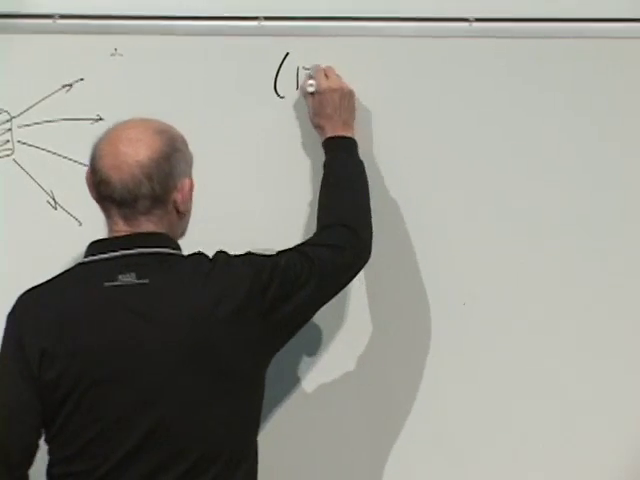
\includegraphics[width=0.66\textwidth]{lecture_06_figure_02.png}
  \caption{Điều kiện vỏ khối lượng trong quy ước metric được dùng xuyên suốt bài giảng.}
  \lectureframe{00:05:56}
  \label{fig:l06-mass-shell}
\end{figure}

Xét hai hạt đi vào với các xung lượng \(k_1,k_2\) và hai hạt đi ra với các xung lượng vật lý \(q_3,q_4\). Bảo toàn năng lượng và xung lượng là một phương trình bốn-véc-tơ,
\begin{equation}
  k_1+k_2=q_3+q_4.
  \label{eq:l06-physical-conservation}
\end{equation}
Thuận tiện hơn là gán một xung lượng đi vào cho mọi đường ngoài:
\begin{equation}
  k_3\equiv-q_3,
  \qquad
  k_4\equiv-q_4.
\end{equation}
Khi đó
\begin{equation}
  k_1+k_2+k_3+k_4=0,
  \label{eq:l06-all-incoming}
\end{equation}
và mọi chân đều thỏa \(k_i^2=-m_i^2\). Các hạt đi ra chỉ có năng lượng âm trong quy ước ghi chép này; các năng lượng vật lý của chúng vẫn dương.

\begin{figure}[H]
  \centering
  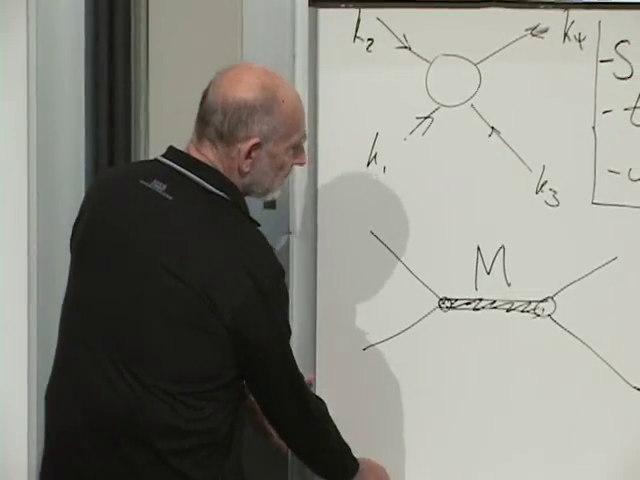
\includegraphics[width=0.68\textwidth]{lecture_06_figure_03.png}
  \caption{Các xung lượng ra vật lý được đảo dấu để cả bốn xung lượng ngoài có thể được xử lý đối xứng như các xung lượng đi vào.}
  \lectureframe{00:09:10}
  \label{fig:l06-all-incoming-board}
\end{figure}

Thoạt đầu, biên độ có vẻ là một hàm của 16 thành phần, \(\mathcal A(k_1,k_2,k_3,k_4)\). Phần lớn trong số đó là thừa. Hãy chuyển sang hệ quy chiếu tâm khối, xoay các xung lượng tới theo một trục đã chọn, và để đơn giản hãy giả sử cả bốn hạt đều có cùng khối lượng. Khi đó trạng thái tới được xác định bởi một đại lượng duy nhất, năng lượng tâm khối. Các xung lượng không gian đi ra phải bằng nhau và ngược chiều nhau, đồng thời có cùng độ lớn với cặp đi vào. Chỉ còn lại góc lệch \(\theta\) của chúng. Vì vậy quá trình có hai biến động học độc lập:
\begin{equation}
  E_{\mathrm{cm}},
  \qquad
  \theta.
  \label{eq:l06-two-data}
\end{equation}

\section{Các biến Mandelstam}

Hai đại lượng vật lý trong \eqref{eq:l06-two-data} phải có thể được biểu diễn mà không cần chọn hệ quy chiếu. Với quy ước mọi hạt đều đi vào, hãy định nghĩa
\begin{equation}
  \begin{aligned}
    -s&=(k_1+k_2)^2,\\
    -t&=(k_1+k_3)^2,\\
    -u&=(k_1+k_4)^2.
  \end{aligned}
  \label{eq:l06-mandelstam}
\end{equation}
Trong hệ tâm khối, các phần không gian của \(k_1+k_2\) triệt tiêu nhau, do đó
\begin{equation}
  s=E_{\mathrm{cm}}^2.
  \label{eq:l06-s-energy}
\end{equation}

Đối với một xung lượng vật lý đi ra \(q_3=-k_3\),
\begin{equation}
  k_1+k_3=k_1-q_3
\end{equation}
là xung lượng truyền từ chân 1 sang chân 3. Với các khối lượng ngoài bằng nhau, và độ lớn xung lượng không gian đi vào là \(p\),
\begin{equation}
  -t=2p^2(1-\cos\theta),
  \qquad
  -u=2p^2(1+\cos\theta).
  \label{eq:l06-tu-angle}
\end{equation}
Vì thế \(t\) và \(u\) mang thông tin góc mà các đầu dò đo được.

\begin{figure}[H]
  \centering
  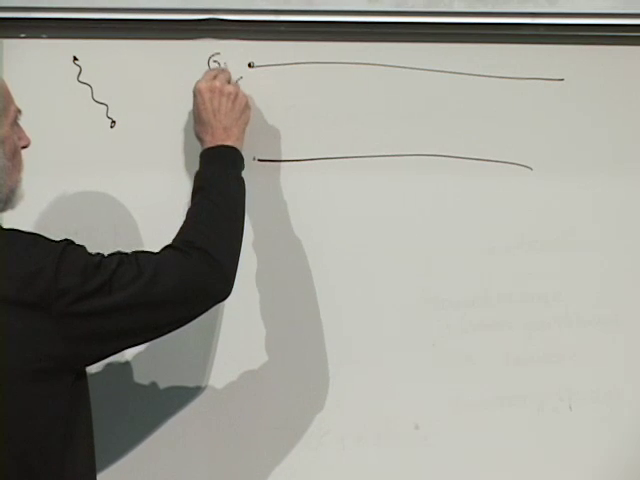
\includegraphics[width=0.74\textwidth]{lecture_06_figure_04.png}
  \caption{Các định nghĩa đối xứng của \(s,t,u\) trong quy ước mọi hạt đều đi vào.}
  \lectureframe{00:26:20}
  \label{fig:l06-stu-board}
\end{figure}

Ba ký hiệu không có nghĩa là ba dữ kiện độc lập. Bình phương \eqref{eq:l06-all-incoming} và dùng \(k_i^2=-m^2\) cho
\begin{equation}
  s+t+u=4m^2
  \label{eq:l06-stu-constraint}
\end{equation}
đối với các khối lượng bằng nhau. Một khi \(s\) và \(t\) đã biết, \(u\) được xác định.

\begin{classroomqa}
\audiencequestion{Liệu chân không có thể làm chậm một hạt chuyển động tự do, gần như ma sát, hay không? \lecturetimestamp{00:27:17}}
\lecturerresponse{Không thể trong một chân không bất biến tịnh tiến. Không có nơi nào để phần xung lượng bị thiếu hụt đi tới, nên bảo toàn xung lượng cấm kiểu ma sát như vậy. Người ta có thể hình dung một môi trường hoặc một chân không khác chọn ra một hệ quy chiếu nghỉ ưu tiên, nhưng đó không phải là chân không đang được dùng ở đây.}
\end{classroomqa}

\begin{classroomqa}
\audiencequestion{Vì sao hai hạt đi ra nhất thiết phải có năng lượng bằng nhau? \lecturetimestamp{00:27:54}}
\lecturerresponse{Trong hệ tâm khối, các xung lượng không gian của chúng phải bằng nhau và ngược chiều nhau. Đối với quá trình khối lượng bằng nhau đang bàn tới, độ lớn xung lượng bằng nhau kéo theo năng lượng bằng nhau theo \(E^2=p^2+m^2\). Nếu các khối lượng đi ra khác nhau, kết luận cuối cùng ấy sẽ phải được sửa đổi.}
\end{classroomqa}

\section{Các kênh trực tiếp và chéo}

Một sơ đồ hạt điểm đơn giản cho phép các hạt 1 và 2 tạo thành một hạt trung gian có khối lượng \(M\), rồi hạt đó phân rã thành 3 và 4. Bỏ qua các thừa số ở tử số và quy tắc cực, sự phụ thuộc đặc trưng của nó là
\begin{equation}
  \mathcal A_s\sim\frac{g^2}{s-M^2}.
  \label{eq:l06-s-channel}
\end{equation}
Đây là quá trình trực tiếp, hay quá trình kênh \(s\). Xoay cách nối sang ngang cho ta sự trao đổi giữa hai đường ngoài,
\begin{equation}
  \mathcal A_t\sim\frac{g^2}{t-M^2},
  \label{eq:l06-t-channel}
\end{equation}
đó là quá trình chéo, hay quá trình kênh \(t\). Một cách nối thứ ba cho
\begin{equation}
  \mathcal A_u\sim\frac{g^2}{u-M^2}.
  \label{eq:l06-u-channel}
\end{equation}

\begin{figure}[H]
  \centering
  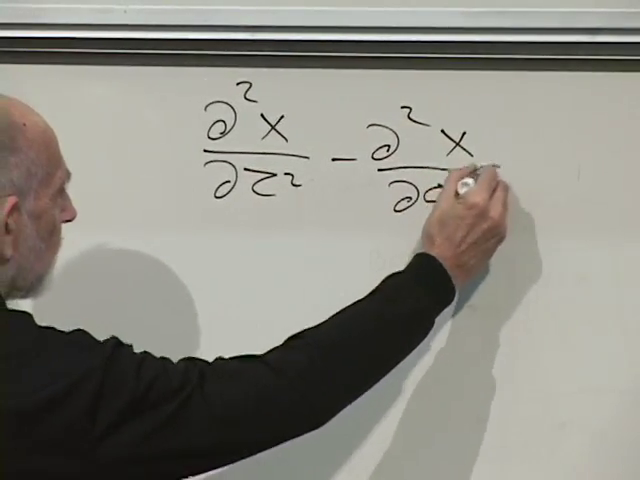
\includegraphics[width=0.72\textwidth]{lecture_06_figure_05.png}
  \caption{Sự tạo thành trực tiếp qua một trạng thái trung gian và cực tương ứng \(g^2/(s-M^2)\); cách nối chéo đang được dựng trên cùng một bảng.}
  \lectureframe{00:30:50}
  \label{fig:l06-channel-board}
\end{figure}

Sự phân biệt này là vật lý. Ở mức vô hướng thô sơ này, \eqref{eq:l06-s-channel} phụ thuộc vào năng lượng va chạm nhưng không phụ thuộc vào góc. Trạng thái hợp thành đã quên hướng tới ban đầu trước khi phân rã, nên sự phân rã của nó là đẳng hướng. Biên độ trao đổi phụ thuộc vào xung lượng truyền và vì thế phụ thuộc vào góc; một hạt trao đổi nhẹ rất thiên về độ lệch nhỏ. Spin sẽ còn bổ sung thêm phụ thuộc góc nữa, nhưng cấu trúc cực đã hiện rõ.

\begin{classroomqa}
\audiencequestion{Kênh \(u\) còn thiếu có sinh ra một hạng thứ ba không? \lecturetimestamp{00:34:47}}
\lecturerresponse{Có, bất cứ khi nào các bản sắc hạt và các ghép nối cho phép cách nối đó. Khi ấy ta thêm một hạng có cực tại \(u=M^2\). Nó không phải là một biến động học độc lập mới, vì \(s+t+u=4m^2\), nhưng nó là một sơ đồ kênh riêng biệt.}
\end{classroomqa}

\section{Một hàm, hai mô tả kênh}

Một cực đơn là một mô hình nghèo nàn của tán xạ meson. Hai meson có thể tạo thành nhiều cộng hưởng, với một tháp các khối lượng và mômen góc. Phản ứng đầu tiên vào những năm 1960 là thêm nhiều cực kênh \(s\) hơn, nhiều cực kênh \(t\) hơn, và các cực kênh \(u\) được phép. Sau đó người ta tìm được một hàm kinh tế hơn nhiều. Trong đơn vị của bài giảng, nơi quỹ đạo Regge tuyến tính và hệ số chặn của nó đã được hấp thụ vào \(s\) và \(t\), hàm đó là
\begin{equation}
  \mathcal A_{\mathrm V}(s,t)
  \propto
  \frac{\Gamma(-s)\Gamma(-t)}{\Gamma(-s-t)}.
  \label{eq:l06-veneziano}
\end{equation}
Hàm gamma mở rộng giai thừa:
\begin{equation}
  \Gamma(n)=(n-1)!
\end{equation}
ở các số nguyên dương.

\begin{figure}[H]
  \centering
  \includegraphics[width=0.68\textwidth]{lecture_06_figure_06.png}
  \caption{Biên độ Veneziano được viết như một tỉ số đối xứng của các hàm gamma.}
  \lectureframe{00:42:25}
  \label{fig:l06-veneziano-board}
\end{figure}

Các cực của \(\Gamma(-s)\) tái tạo một tháp vô hạn các cộng hưởng kênh trực tiếp. Tuy vậy, chính biểu thức ấy lại đối xứng dưới \(s\leftrightarrow
t\), nên các cực \(\Gamma(-t)\) của nó cho một khai triển theo kênh chéo. Đây không phải là hai đóng góp được cộng vào một cách riêng rẽ. Một hàm giải tích duy nhất chấp nhận một trong hai mô tả. Đó là ý tưởng cổ điển về đối ngẫu giữa các cộng hưởng kênh trực tiếp và các trao đổi kênh chéo.

\begin{classroomqa}
\audiencequestion{Làm sao một biên độ có thể chứa cả hai tổng theo kênh mà không cần cộng chúng lại? \lecturetimestamp{00:43:32}}
\lecturerresponse{Chính đó mới là điều bất ngờ. Khai triển hàm gần các cực kênh \(s\) của nó sẽ tổ chức nó thành các cộng hưởng trực tiếp; khai triển gần các cực kênh \(t\) của nó sẽ tổ chức chính hàm ấy thành các trao đổi. Cần có một mô hình vi mô để giải thích vì sao hai cách đọc đó lại là một, và mô hình ấy là một dây tương tác.}
\end{classroomqa}

\section{Một dải do một dây mở quét ra}

Tham số hóa một dây mở bằng
\begin{equation}
  0\leq\sigma\leq\pi.
\end{equation}
Nhãn \(\sigma\) không phải là một vị trí trong không-thời gian. Phép nhúng \(X^\mu(\sigma,\tau)\) cho ta biết điểm mang nhãn đó nằm ở đâu trong không-thời gian, còn \(\tau\) đo sự tiến hóa. Một hạt điểm quét ra một đường thế giới; dây đang chuyển động quét ra một mặt thế giới hai chiều. Trong lý thuyết tự do, mỗi tọa độ nhúng đều thỏa
\begin{equation}
  \frac{\partial^2X^\mu}{\partial\tau^2}
  -
  \frac{\partial^2X^\mu}{\partial\sigma^2}
  =0.
  \label{eq:l06-wave-equation}
\end{equation}

\begin{figure}[H]
  \centering
  \includegraphics[width=0.70\textwidth]{lecture_06_figure_07.png}
  \caption{Phương trình sóng chi phối mỗi tọa độ của dây tự do trên dải mặt thế giới.}
  \lectureframe{00:49:10}
  \label{fig:l06-wave-equation-board}
\end{figure}

Đối với việc xây dựng tán xạ, sẽ có ích nếu chưa vội lấy giới hạn liên tục. Hãy thay mỗi dây bằng \(n\) điểm khối lượng nối với nhau bằng các lò xo. Mặt thế giới trở thành một tập dày đặc các đường thế giới kề nhau, và các mode chuẩn của nó là các dao động tử điều hòa thông thường. Hai chuỗi tới có thể chạm nhau ở các đầu mút. Tại biến cố ấy, một lò xo mới nối chúng lại, chúng tiến hóa trong một khoảng \(\tau\) như một chuỗi dài hơn duy nhất, rồi về sau một lò xo đứt ra để hai chuỗi đi ra xuất hiện.

\begin{figure}[H]
  \centering
  \includegraphics[width=0.72\textwidth]{lecture_06_figure_08.png}
  \medskip

\begin{tikzpicture}[x=0.85cm,y=0.70cm]
    \draw[thick] (0,2.2) -- (2.1,2.2) -- (3.1,1.5);
    \draw[thick] (0,0.8) -- (2.1,0.8) -- (3.1,1.5);
    \draw[thick] (3.1,1.5) -- (5.5,1.5);
    \draw[thick] (5.5,1.5) -- (6.5,2.2) -- (8.6,2.2);
    \draw[thick] (5.5,1.5) -- (6.5,0.8) -- (8.6,0.8);
    \draw[<->] (3.1,0.35) -- node[below] {\(\tau\)} (5.5,0.35);
    \node[left] at (0,2.2) {1};
    \node[left] at (0,0.8) {2};
    \node[right] at (8.6,2.2) {3};
    \node[right] at (8.6,0.8) {4};
  \end{tikzpicture}
  \caption{Hai dây mở được rời rạc hóa chạm nhau, tạo thành một dây trung gian trong khoảng \(\tau\), rồi tách ra. Khung hình gốc giữ nguyên cấu trúc lò xo và đường thế giới; hình sơ đồ tách riêng cách nối của nó.}
  \lectureframe{00:51:25}
  \label{fig:l06-string-joining}
\end{figure}

Hai dây chỉ được vẽ kề nhau trong không gian tham số. Các vị trí của chúng trong không-thời gian không nhất thiết phải kề nhau cho đến khi các tọa độ đầu mút thực sự trùng nhau. Tự do tái tham số hóa cho phép đặt các biến cố nối và tách tại những vị trí thuận tiện trên hình; sự tự do hình học này sẽ trở thành đối xứng bảo giác trong bài giảng tiếp theo.

\section{Phép tính dao động tử từng bước}

Gọi các tọa độ của chuỗi thứ nhất là \(x_1,\ldots,x_n\), và của chuỗi thứ hai là \(x_{n+1},\ldots,x_{2n}\). Tọa độ tâm khối của chúng là
\begin{equation}
  X_{\mathrm{cm}}^{(1)}
  =\frac1n\sum_{a=1}^{n}x_a,
  \qquad
  X_{\mathrm{cm}}^{(2)}
  =\frac1n\sum_{a=n+1}^{2n}x_a.
  \label{eq:l06-chain-centers}
\end{equation}
Một chuỗi có xung lượng xác định \(k_1\) có một sóng phẳng tâm khối nhân với một trạng thái cơ bản dao động tử nội tại:
\begin{align}
  \Psi_1
  &=
  e^{ik_1\cdot X_{\mathrm{cm}}^{(1)}}
  \psi_0(x_1,\ldots,x_n),
  \\
  \Psi_2
  &=
  e^{ik_2\cdot X_{\mathrm{cm}}^{(2)}}
  \psi_0(x_{n+1},\ldots,x_{2n}).
  \label{eq:l06-two-wavefunctions}
\end{align}
Các thừa số \(\psi_0\) phụ thuộc vào các tọa độ tương đối, chứ không phụ thuộc vào phép tịnh tiến chung của cả chuỗi. Vì các dây tới lúc đầu là những hệ lượng tử tách biệt,
\begin{equation}
  \Psi_{\mathrm{in}}=\Psi_1\Psi_2.
  \label{eq:l06-product-state}
\end{equation}

\begin{figure}[H]
  \centering
  \includegraphics[width=0.76\textwidth]{lecture_06_figure_09.png}
  \caption{Hai sóng phẳng xung lượng và các thừa số trạng thái cơ bản dao động tử nội tại của chúng, được viết bằng các màu khác nhau.}
  \lectureframe{00:58:05}
  \label{fig:l06-wavefunctions-board}
\end{figure}

Sự nối chọn ra phần của hàm sóng này mà tại đó hai tọa độ đầu mút trùng nhau:
\begin{equation}
  x_n=x_{n+1}.
  \label{eq:l06-endpoint-contact}
\end{equation}
Ở thời điểm đó, các tọa độ khác không đổi. Trạng thái được chọn sau đó được cho tiến hóa bằng Hamiltonian \(H_{\mathrm{joined}}\) của chuỗi dài hơn duy nhất:
\begin{equation}
  \Psi(\tau)
  =
  e^{-iH_{\mathrm{joined}}\tau}\Psi(0).
  \label{eq:l06-time-evolution}
\end{equation}
Cuối cùng, ta lấy độ chồng lấp của nó với tích các trạng thái dây đi ra mang xung lượng \(q_3,q_4\).

\begin{figure}[H]
  \centering
  \includegraphics[width=0.76\textwidth]{lecture_06_figure_10.png}
  \caption{Hàm sóng hai chuỗi ngay trước khi điều kiện trùng nhau của các đầu mút được áp đặt.}
  \lectureframe{00:58:55}
  \label{fig:l06-endpoint-board}
\end{figure}

Phép tính thì dài nhưng không bí hiểm. Mỗi tọa độ nội tại đều có thể được phân rã thành các mode dao động tử, nên độ chồng lấp khi nối, sự tiến hóa theo thời gian và phép chiếu cuối cùng đều quy về đại số Gaussian của các dao động tử. Điều còn chưa được cố định là thời gian sống \(\tau\) của dây đã nối.

\begin{classroomqa}
\audiencequestion{Các hàm sóng màu đen và đỏ được cộng hay nhân với nhau? \lecturetimestamp{01:02:26}}
\lecturerresponse{Nhân. Trạng thái tích tensor của hai hệ độc lập được biểu diễn trong cơ sở tọa độ bằng tích các hàm sóng của chúng. Phép cộng sẽ mô tả một chồng chập của các khả năng, chứ không phải sự hiện diện đồng thời của cả hai dây đi vào.}
\end{classroomqa}

\begin{classroomqa}
\audiencequestion{Tại sao lại lấy tích phân theo thời gian trung gian
\(\tau\)? \lecturetimestamp{01:04:04}}
\lecturerresponse{Không gán cho dây đã nối một thời gian sống cố định.
Quy tắc của Feynman là cộng các biên độ trên mọi lịch sử được phép. Trong mô tả này, tham số lịch sử liên tục còn lại là thời gian giữa lúc nối và lúc tách, nên tổng trở thành một tích phân trên
\(0\leq\tau<\infty\).}
\end{classroomqa}

\section{Từ thời gian truyền đến hàm beta}

Sau khi tính các độ chồng lấp của các dao động tử, kết quả có thể được sắp xếp thành
\begin{equation}
  \mathcal A(s,t)
  \propto
  \int_0^\infty d\tau\,
  e^{\tau(s+1)}
  \bigl(1-e^{-\tau}\bigr)^{-t-1}
  e^{-\tau}.
  \label{eq:l06-tau-integral}
\end{equation}
Thừa số \(e^{-\tau}\) ở cuối được giữ tường minh vì đó là nhân tử Jacobi cần cho bước tiếp theo. Tương đương, các hàm mũ thứ nhất và cuối cùng kết hợp thành
\(e^{s\tau}\).

\begin{figure}[H]
  \centering
  \includegraphics[width=0.76\textwidth]{lecture_06_figure_11.png}
  \caption{Biểu thức dưới dấu tích phân theo thời gian truyền sau phép tính dao động tử;
  thừa số \(e^{-\tau}\) tách riêng cung cấp nhân tử Jacobi
  cho phép đổi biến.}
  \lectureframe{01:06:45}
  \label{fig:l06-tau-integral-board}
\end{figure}

Bây giờ đặt
\begin{equation}
  z=e^{-\tau},
  \qquad
  dz=-e^{-\tau}\,d\tau.
  \label{eq:l06-z-substitution}
\end{equation}
Khi \(\tau\) chạy từ \(0\) đến \(\infty\), \(z\) chạy từ \(1\) đến \(0\).
Dấu trừ đảo ngược các cận, do đó thu được
\begin{equation}
  \mathcal A(s,t)
  \propto
  \int_0^1
  z^{-s-1}(1-z)^{-t-1}\,dz.
  \label{eq:l06-beta-integral}
\end{equation}

\begin{figure}[H]
  \centering
  \includegraphics[width=0.74\textwidth]{lecture_06_figure_12.png}
  \caption{Phép thế \(z=e^{-\tau}\) làm lộ ra tích phân beta
  Euler.}
  \lectureframe{01:08:49}
  \label{fig:l06-beta-integral-board}
\end{figure}

Tích phân này được xác định trực tiếp trong miền mà nó hội tụ tại các đầu mút, và ở những miền khác thì bằng phép tiếp tục giải tích. Nó chính là hàm beta Euler:
\begin{equation}
  B(-s,-t)
  =
  \frac{\Gamma(-s)\Gamma(-t)}{\Gamma(-s-t)}.
  \label{eq:l06-beta-gamma}
\end{equation}

\begin{figure}[H]
  \centering
  \includegraphics[width=0.72\textwidth]{lecture_06_figure_13.png}
  \caption{Trên bảng, tích phân đã biến đổi được đồng nhất với
  \(B(-s,-t)\) và bắt đầu được viết lại về dạng hàm gamma của nó.}
  \lectureframe{01:12:24}
  \label{fig:l06-beta-gamma-board}
\end{figure}

Đối xứng kênh giờ đây trở nên hiển nhiên. Dưới phép biến đổi \(z\mapsto1-z\),
\begin{equation}
  \int_0^1 z^{-s-1}(1-z)^{-t-1}\,dz
  =
  \int_0^1 z^{-t-1}(1-z)^{-s-1}\,dz.
\end{equation}
Vì thế \(\mathcal A(s,t)=\mathcal A(t,s)\). Một quá trình được xây dựng như hai dây nối lại rồi sau đó tách ra tự động cũng chứa mô tả kênh chéo.
\editorialnote{Bài giảng lược bỏ độ dốc Regge và hệ số chặn trong các đối số của hàm beta. Trong ký hiệu chuẩn, người ta thay \(s,t\)
bằng các quỹ đạo tuyến tính tương ứng \(\alpha(s),\alpha(t)\). Tính đối ngẫu và lập luận đổi biến không thay đổi.}

\begin{classroomqa}
\audiencequestion{Tỷ số các hàm gamma trông giống những biểu thức
giai thừa trong tổ hợp học. Có một cách diễn giải đếm trực tiếp
về mặt vật lý nào không? \lecturetimestamp{01:13:22}}
\lecturerresponse{Với các đối số nguyên, hàm beta liên hệ với một
tỷ số như \(n!\,m!/(n+m)!\), nhưng ở đây không hề khẳng định có một
cơ chế tổ hợp nào. Cùng một hàm đặc biệt đó cũng xuất hiện từ tích phân
trên mặt thế giới; sự giống nhau này không phải là con đường đã dẫn tới việc tìm ra
biên độ.}
\end{classroomqa}

Lý do còn chưa lộ ra khiến một mặt thế giới có thể được diễn giải theo cả hai kênh là đối xứng bảo giác. Nó cho phép mặt ấy bị kéo giãn như kẹo kéo mà không làm thay đổi biên độ, biến một vùng truyền dài của kênh trực tiếp thành một bức tranh trao đổi ở kênh chéo. Cách giải thích hình học đó được dời sang bài giảng tiếp theo.

\section{Phép kiểm tra tán xạ đã xác lập điều gì}
\enlargethispage{3\baselineskip}
\begingroup
\setlength{\medskipamount}{3pt plus 1pt minus 1pt}

Bức tranh nối rời rạc đã gợi ra một loạt câu hỏi cuối cùng.

\begin{classroomqa}
\audiencequestion{Nếu hai chuỗi, mỗi chuỗi gồm \(n\) thành phần, nối nhau tại các
đầu mút, thì kết quả có phải là \(2n-1\) không, và điều đó có thể làm thay đổi chẵn lẻ
fermion không? \lecturetimestamp{01:16:16}}
\lecturerresponse{Trong bức tranh hadron ở đầu mút, cặp đầu mút tiếp xúc
có thể được xem như một cặp hạt-phản hạt hủy nhau, nên
số đếm giảm đi hai chứ không phải một. Trong giới hạn liên tục, sai khác hữu hạn giữa \(2n\) và \(2n-2\) là không quan trọng, nhưng việc bảo toàn chẵn lẻ fermion
thì không phải vậy. Các thành phần trên mạng chỉ là một bộ điều chuẩn cho
dây liên tục, chứ không phải những hạt cườm cơ bản theo nghĩa đen.}
\end{classroomqa}

\begin{classroomqa}
\audiencequestion{Phần thảo luận về sau có đi tiếp vào toàn bộ
toán học của siêu dây không? \lecturetimestamp{01:18:05}}
\lecturerresponse{Chỉ một số hệ quả chọn lọc sẽ được dùng. Lộ trình trước mắt
đi qua đối xứng mặt thế giới và compact hóa, tiếp theo là một
điểm xuất phát khác được phát triển vào giữa thập niên 1990: M-lý thuyết. Mục đích
của nó là đi tới cùng một vật lý từ một quan điểm trong đó một số đặc điểm vốn dĩ
phức tạp trở nên minh bạch.}
\end{classroomqa}

\begin{classroomqa}
\audiencequestion{Quy tắc nối này chỉ là một gợi ý từ các va chạm
meson thôi sao? \lecturetimestamp{01:20:02}}
\lecturerresponse{Tán xạ meson cung cấp gợi ý về mặt lịch sử, nhưng
quy tắc này là tổng quát đối với dây hở. Cùng một tôpô mô tả các va chạm của
photon của dây hở và các trạng thái dây hở khác. Hai dây kín nối lại
rồi tách ra bằng một cách xây dựng tương tự, với một dây kín ở vùng
trung gian.}
\end{classroomqa}

\begin{classroomqa}
\audiencequestion{Phép tính này chỉ áp dụng khi các trạng thái dây là
fermion thôi sao? \lecturetimestamp{01:20:56}}
\lecturerresponse{Không. Phép tính Veneziano ban đầu thuộc về
dây hở boson. Siêu dây đòi hỏi thêm các bậc tự do fermion và
làm thay đổi chi tiết của biểu thức dưới dấu tích phân, nhưng logic về sự nối, sự truyền,
phép chiếu và đối ngẫu mặt thế giới vẫn gần như tương tự.}
\end{classroomqa}

Việc tìm thấy một trạng thái spin một hay spin hai trong phổ dao động tử là gợi ý, nhưng chưa có tính quyết định. Biên độ tán xạ của chúng mới cung cấp phép kiểm tra mạnh hơn. Các biên độ photon tuân theo những đồng nhất thức gắn với bảo toàn điện tích và bất biến chuẩn; các biên độ graviton tuân theo những ràng buộc tương ứng của một trường spin hai không khối lượng. Các trạng thái dây đã vượt qua những phép kiểm tra này trong tương tác với các trạng thái có khối lượng, các trạng thái không khối lượng, và với nhau.
Đó là lý do vì sao các nhãn photon và graviton trở thành những nhận diện vật lý chứ không phải những phỏng đoán chỉ dựa trên việc đếm phân cực.
\editorialnote{Theo ngôn ngữ hiện đại, các phép kiểm tra này được mã hóa trong sự tách rời của các phân cực phi vật lý, các đồng nhất thức Ward chuẩn, và sự ghép nối năng lượng thấp phổ quát của trạng thái spin hai không khối lượng.}

\begin{classroomqa}
\audiencequestion{Bản thân điện tích phát sinh từ đâu trong mô tả
dây? \lecturetimestamp{01:24:03}}
\lecturerresponse{Câu hỏi đó được để ngỏ ở cuối bài giảng. Câu
trả lời cho nó đòi hỏi cấu trúc nội tại và cấu trúc đầu mút của lý thuyết dây,
những điều vẫn chưa được giới thiệu, nên nó thuộc về phần thảo luận tiếp theo chứ không thuộc phép suy dẫn tán xạ này.}
\end{classroomqa}
\endgroup

\chapter{Các mặt thế giới, phép quay Wick và tính đối ngẫu giữa các kênh}

\lectureoverview{Một hạt vạch ra một đường thế giới; một dây quét ra một mặt thế giới. Việc lượng tử hóa một trong hai đối tượng đòi hỏi lấy tổng trên các lịch sử, nhưng tổng Lorentz dao động và khó xác định. Biến thời gian của mặt thế giới thành một tọa độ ảo cho ta một lý thuyết Euclid được chi phối bởi phương trình Laplace. Đối xứng bảo giác của nó khi đó biến mặt có khe của một tương tác bốn dây thành một đĩa với bốn điểm chèn trên biên, nơi sự đối xứng giữa kênh trực tiếp và kênh chéo trở nên hiển hiện.}

\section{Từ một đường thế giới đến tổng trên các lịch sử}

Hãy bắt đầu với một hạt tự do. Trong cơ học phi tương đối tính, vị trí của nó là một hàm \(\mathbf x(t)\), và khi đặt khối lượng bằng một, tác dụng của nó là
\begin{equation}
  S_{\mathrm{NR}}[\mathbf x]
  =\frac12\int_{t_1}^{t_2}\dot{\mathbf x}^{\,2}\,dt.
  \label{eq:l07-nr-action}
\end{equation}
Đối với mô tả tương đối tính, tự nhiên hơn là gộp thời gian và không gian vào một vectơ, \(X^\mu(\tau)\), được tham số hóa dọc theo quỹ đạo bởi \(\tau\). Biểu thức bậc hai tương ứng là
\begin{equation}
  S_{\mathrm{rel}}[X]
  =\frac12\int_{\tau_1}^{\tau_2}
  \frac{dX^\mu}{d\tau}\frac{dX_\mu}{d\tau}\,d\tau.
  \label{eq:l07-rel-action}
\end{equation}
Các chỉ số trên và dưới mã hóa sự khác biệt dấu kiểu Lorentz giữa thời gian và không gian.
\editorialnote{Ở đây tác dụng tương đối tính bậc hai được dùng trong một cách tham số hóa đường thế giới cố định. Lựa chọn thay thế hiển nhiên bất biến đối với phép đổi tham số thì tỉ lệ với độ dài riêng, và sẽ được nhắc đến ở phần sau của bài giảng.}

\begin{figure}[H]
  \centering
  \includegraphics[width=0.72\textwidth]{lecture_07_figure_01.png}
  \caption{Tác dụng phi tương đối tính và dạng tương ứng bậc hai tương đối tính của nó được viết cùng nhau trên bảng.}
  \lectureframe{00:03:35}
  \label{fig:l07-particle-actions}
\end{figure}

Về mặt cổ điển, ta cố định hai đầu mút và biến thiên đường đi. Khi đó một hạt tự do đi theo một đường thế giới thẳng với vận tốc không đổi. Cơ học lượng tử đặt ra một câu hỏi khác. Nó không chọn ra một quỹ đạo giữa hai đầu mút; nó hỏi biên độ để hạt bắt đầu ở một điểm và được phát hiện ở điểm kia là bao nhiêu. Mọi đường đi xen giữa đều đóng góp một pha,
\begin{equation}
  K(2,1)=\int_{X(1)}^{X(2)}\!\mathcal D X\,
  e^{iS[X]}.
  \label{eq:l07-feynman-integral}
\end{equation}
Tích phân hàm là một tích phân trên một không gian vô hạn chiều của các đường đi, chứ không phải tích phân thông thường đã xuất hiện bên trong tác dụng.

\begin{figure}[H]
  \centering
  \includegraphics[width=0.72\textwidth]{lecture_07_figure_02.png}
  \caption{Một đường đi tiêu biểu và pha được gán cho nó trước khi lấy tổng trên mọi đường đi.}
  \lectureframe{00:06:21}
  \label{fig:l07-path-integral-board}
\end{figure}

Trong ngôn ngữ tương đối tính, biên độ từ điểm này đến điểm kia là một hàm truyền. Đối với một tương tác, nhiều đoạn đường thế giới gặp nhau. Các tác dụng của chúng được cộng lại, các điểm gặp được lấy tích phân, và ta lấy tổng các giản đồ có những hạt ngoài cần thiết. Vì thế, khai triển quen thuộc theo giản đồ Feynman đã hàm ẩn ngay trong chỉ dẫn lấy tổng trên các lịch sử.

Ở đây, ký hiệu \(S\) sẽ dùng để chỉ tác dụng. Nó không liên quan cả đến entropy lẫn biến Mandelstam \(s\) được dùng gần cuối bài giảng. Việc dùng chung ký hiệu này là do truyền thống hơn là do nó làm sáng tỏ điều gì.

\section{Xoay thời gian sang ngang}

Có một vấn đề nảy sinh ngay với \eqref{eq:l07-feynman-integral}. Mỗi thừa số \(e^{iS}\) đều có độ lớn bằng một. Vì vậy, một quỹ đạo dao động dữ dội và đường thẳng cổ điển đều đi vào với cùng trọng số tuyệt đối; chỉ pha của chúng là khác nhau. Giao thoa triệt tiêu khôi phục hành vi cổ điển, nhưng nó không biến tích phân hình thức ấy thành một đối tượng hội tụ thông thường.

Đưa vào một tham số mới \(s\) theo
\begin{equation}
  \tau=\alpha s,
  \qquad
  d\tau=\alpha\,ds,
  \qquad
  \frac{dX}{d\tau}=\frac{1}{\alpha}\frac{dX}{ds}.
\end{equation}
Khi đó tác dụng bậc hai đổi tỉ lệ thành
\begin{equation}
  \frac12\int d\tau
  \left(\frac{dX}{d\tau}\right)^2
  =
  \frac{1}{2\alpha}\int ds
  \left(\frac{dX}{ds}\right)^2.
  \label{eq:l07-rescaled-action}
\end{equation}
Chọn đường bao tương ứng với \(\alpha=-i\) sẽ biến trọng số dao động thành
\begin{equation}
  e^{iS}
  \longrightarrow
  \exp\!\left[-\frac12\int ds
  \left(\frac{dX}{ds}\right)^2\right]
  =e^{-S_E}.
  \label{eq:l07-euclidean-particle}
\end{equation}

\begin{figure}[H]
  \centering
  \includegraphics[width=0.66\textwidth]{lecture_07_figure_03.png}
  \caption{Trọng số Euclid của hạt sau phép thế thời gian ảo; số mũ là thực và không dương.}
  \lectureframe{00:16:20}
  \label{fig:l07-particle-wick}
\end{figure}

Một đường đi chạy ra rất xa rồi quay lại, hoặc uốn lượn nhanh mà không đi xa, có \(S_E\) dương lớn và bị triệt giảm theo hàm mũ. Kết quả là một tích phân kiểu Wiener, đối với nó tồn tại một lý thuyết hội tụ nghiêm túc. Các đầu mút kế thừa từ \(\tau\) thực nằm trên một đường bao \(s\) ảo. Trong thực hành, người ta tính đối tượng Euclid trong miền hội tụ của nó rồi tiếp tục giải tích kết quả trở lại các biến Lorentz vật lý. Phép toán này là phép quay Wick: thời gian đã được xoay sang bên để phục vụ phép tính, chứ không bị loại bỏ.

\section{Từ các đường thế giới đến các mặt thế giới}

Một hạt điểm có một đường thế giới. Một dây mở quét ra một dải, còn một dây kín quét ra một ống. Các tọa độ \((\sigma,\tau)\) gắn nhãn các điểm trên mặt thế giới hai chiều này, còn
\begin{equation}
  X^\mu=X^\mu(\sigma,\tau)
  \label{eq:l07-embedding}
\end{equation}
cho vị trí không-thời gian của điểm mang nhãn đó. Biết toàn bộ các hàm \(X^\mu\) là xác định đầy đủ lịch sử của dây.

Tác dụng Lorentz bậc hai của mặt thế giới có cùng cấu trúc động năng trừ thế năng như một dây dao động thông thường:
\begin{equation}
  S_{\mathrm{ws}}[X]
  =\frac{T_s}{2}\int d\tau\,d\sigma\,
  \left[
    \partial_\tau X^\mu\partial_\tau X_\mu
    -
    \partial_\sigma X^\mu\partial_\sigma X_\mu
  \right].
  \label{eq:l07-lorentzian-worldsheet}
\end{equation}
Sức căng tổng thể \(T_s\) ấn định thang đo; bài giảng lược bỏ nó để tập trung vào cấu trúc đạo hàm.

\begin{figure}[H]
  \centering
  \includegraphics[width=0.72\textwidth]{lecture_07_figure_04.png}
  \caption{Tác dụng mặt thế giới Lorentz cho
  \(X^\mu(\sigma,\tau)\), với dấu động năng trừ thế năng của nó.}
  \lectureframe{00:24:26}
  \label{fig:l07-worldsheet-action}
\end{figure}

Biên độ của dây được thu được bằng cách mũ hóa tác dụng này và lấy tổng trên mọi mặt nối các cấu hình dây đầu và cuối đã cho:
\begin{equation}
  \mathcal A=\int\mathcal D X\,e^{iS_{\mathrm{ws}}[X]}.
  \label{eq:l07-surface-integral}
\end{equation}
Quy tắc ấy cũng xử lý trường hợp hai dây thành hai, hai thành ba, hoặc bất kỳ cấu hình ngoài nào khác được phép. Các tôpô mặt thế giới khác nhau cũng thuộc vào tổng này. Việc thêm các lỗ là đối tác phía dây của việc thêm các bậc vòng trong khai triển giản đồ hạt điểm.

\begin{figure}[H]
  \centering
  \includegraphics[width=0.66\textwidth]{lecture_07_figure_05.png}
  \caption{Một mặt nối nhiều dây ngoài, với một lỗ biểu diễn một tôpô mặt thế giới khác.}
  \lectureframe{00:27:14}
  \label{fig:l07-surface-topology}
\end{figure}

\begin{classroomqa}
\audiencequestion{Đối với một electron điểm, đạo hàm theo \(\sigma\) có đơn giản là triệt tiêu không? \lecturetimestamp{00:27:56}}
\lecturerresponse{Trước hết, một hạt điểm vốn không có tọa độ \(\sigma\). Tuy vậy, hai bức tranh có liên hệ với nhau: khi các trạng thái ngoài nhẹ so với thang dây và năng lượng của quá trình thấp, các biên độ dây tái tạo các giản đồ Feynman hạt điểm thông thường. Giới hạn đó còn nhiều hơn việc cho một đạo hàm bằng 0.}
\end{classroomqa}

Tích phân trên mặt có cùng vấn đề hội tụ như tích phân đường đi. Sau khi quay Wick thời gian mặt thế giới, dạng Euclid ổn định của nó là
\begin{equation}
  \begin{aligned}
    S_{E,\mathrm{ws}}[X]
    &=\frac{T_s}{2}\int d\tau\,d\sigma\,
      \left[
        \partial_\tau X^\mu\partial_\tau X_\mu
        +\partial_\sigma X^\mu\partial_\sigma X_\mu
      \right],\\
    \mathcal A_E&=\int\mathcal D X\,e^{-S_{E,\mathrm{ws}}}.
  \end{aligned}
  \label{eq:l07-euclidean-worldsheet}
\end{equation}
Giờ đây cả hai đạo hàm đều đi vào với cùng dấu dương. Một mặt dao động dữ dội hoặc bị kéo căng mạnh có tác dụng Euclid lớn và bị triệt giảm.

\begin{figure}[H]
  \centering
  \includegraphics[width=0.72\textwidth]{lecture_07_figure_06.png}
  \caption{Mật độ mặt thế giới Euclid dương sau khi
  \(\tau\) được quay sang thời gian ảo.}
  \lectureframe{00:34:29}
  \label{fig:l07-worldsheet-wick}
\end{figure}

Cũng có một cách phát biểu trực tiếp về mặt hình học. Có thể gán cho một hạt tương đối tính một tác dụng tỉ lệ với độ dài riêng của quỹ đạo nó; có thể gán cho một dây một tác dụng tỉ lệ với diện tích không-thời gian của mặt thế giới của nó. Dạng sau là tác dụng Nambu--Goto. Dạng mặt thế giới bậc hai được dùng ở đây theo quy ước được gọi là dạng Polyakov và dễ hơn nhiều cho phép tính hiện tại.
\editorialnote{Bài giảng có kèm một trao đổi hài hước về cách đặt tên trong lịch sử và cũng nhắc đến tác dụng Liouville liên quan cùng các điều kiện biên Dirichlet. Việc suy dẫn không cần đến bất kỳ khẳng định ưu tiên nào: chỉ dùng sự tương đương giữa mô tả theo diện tích và mô tả với metric phụ trợ.}

\section{Phương trình chuyển động Euclid}

Các tọa độ \(\sigma\) và \(\tau\) chỉ là các nhãn trên mặt. Vì vậy câu hỏi tiếp theo là không thể tránh khỏi: những phép gắn nhãn lại nào để nguyên lý thuyết? Câu trả lời dễ thấy nhất từ phương trình chuyển động. Biến phân \eqref{eq:l07-euclidean-worldsheet} cho, theo từng thành phần,
\begin{equation}
  \partial_\tau^2X^\mu+\partial_\sigma^2X^\mu=0.
  \label{eq:l07-laplace}
\end{equation}
Trước phép quay Wick, dấu tương đối là âm và đây là một phương trình sóng. Trong chữ ký Euclid, cả hai dấu đều dương, nên đây là phương trình Laplace hai chiều.

\begin{classroomqa}
\audiencequestion{Đây có phải là phương trình của một màng trống dao động không?
\lecturetimestamp{00:41:50}}
\lecturerresponse{Nó có liên hệ rất gần, nhưng một màng trống dao động còn có một tọa độ thời gian thực và vì thế tuân theo một phương trình sóng. Phương trình ở đây là phương trình Laplace Euclid. Thế điện tĩnh trong một miền không có điện tích cho một ví dụ quen thuộc trực tiếp hơn.}
\end{classroomqa}

\begin{classroomqa}
\audiencequestion{Tác dụng chứa các đạo hàm bậc nhất. Vì sao phương trình của nó lại chứa các đạo hàm bậc hai? \lecturetimestamp{00:42:44}}
\lecturerresponse{Biến phân một hạng tử bậc hai theo đạo hàm bậc nhất rồi lấy tích phân từng phần sẽ chuyển một đạo hàm lên đạo hàm bậc nhất ấy. Đây là phiên bản của lý thuyết trường trong đó \(\dot x^{\,2}\) ở trong tác dụng sinh ra \(\ddot x\) trong phương trình chuyển động.}
\end{classroomqa}

\begin{figure}[H]
  \centering
  \includegraphics[width=0.68\textwidth]{lecture_07_figure_07.png}
  \caption{Phương trình Laplace với dấu cộng và dòng rời rạc đầu tiên được dùng để diễn giải các đạo hàm bậc hai của nó.}
  \lectureframe{00:43:30}
  \label{fig:l07-laplace-board}
\end{figure}

Để thấy hình học, trước hết hãy rời rạc hóa một tọa độ với khoảng cách \(\epsilon\). Đạo hàm bậc nhất là hiệu giữa các điểm lân cận, còn đạo hàm bậc hai là hiệu của các hiệu lân cận:
\begin{equation}
  \frac{d^2X}{ds^2}\bigg|_{2}
  \longrightarrow
  \frac{X(3)-2X(2)+X(1)}{\epsilon^2}.
  \label{eq:l07-second-difference}
\end{equation}

\begin{figure}[H]
  \centering
  \includegraphics[width=0.72\textwidth]{lecture_07_figure_08.png}
  \caption{Đường thẳng được đánh số, một mảnh lưới nhỏ và khai triển sai phân hữu hạn của một đạo hàm bậc hai.}
  \lectureframe{00:45:51}
  \label{fig:l07-finite-difference-board}
\end{figure}

Bây giờ hãy rời rạc hóa mặt phẳng \((\sigma,\tau)\). Gắn nhãn bốn điểm lân cận gần nhất của điểm trung tâm \(5\) là \(1,2,3,4\). Phương trình \eqref{eq:l07-laplace} trở thành
\begin{equation}
  X(1)+X(2)+X(3)+X(4)-4X(5)=0,
\end{equation}
hay
\begin{equation}
  X(5)=\frac14\bigl[X(1)+X(2)+X(3)+X(4)\bigr].
  \label{eq:l07-mean-value}
\end{equation}

\begin{figure}[H]
  \centering
  \includegraphics[width=0.72\textwidth]{lecture_07_figure_09.png}
  \caption{Phương trình sai phân hữu hạn hai chiều hoàn chỉnh: giá trị ở tâm bằng trung bình của bốn điểm lân cận của nó.}
  \lectureframe{00:48:26}
  \label{fig:l07-mean-value-board}
\end{figure}

Tính chất giá trị trung bình này đúng cho một hình vuông vi phân ở mọi định hướng. Đó là nội dung hình học địa phương của phương trình Laplace và là chiếc cầu nối tới đối xứng bảo giác.

\section{Tọa độ bảo giác}

Xét một phép đổi từ \((\sigma,\tau)\) sang
\((\sigma',\tau')\). Một biến dạng tổng quát biến một hình vuông nhỏ thành một tứ giác tùy ý. Những phép biến đổi đặc biệt có liên quan ở đây biến mọi hình vuông vi phân thành một hình vuông vi phân khác, có thể bị quay và đổi tỉ lệ. Tương đương, chúng bảo toàn các góc mà tại đó các đường cong gặp nhau. Đó là các phép biến đổi bảo giác.

\begin{figure}[H]
  \centering
  \includegraphics[width=0.68\textwidth]{lecture_07_figure_10.png}
  \caption{Một hình vuông địa phương được ánh xạ sang một hình nhỏ khác, đồng thời kiểm tra xem các góc của nó có được bảo toàn theo nghĩa bảo giác hay không.}
  \lectureframe{00:53:25}
  \label{fig:l07-conformal-board}
\end{figure}

\begin{classroomqa}
\audiencequestion{Nếu các góc được bảo toàn, về cơ bản phép biến đổi có phải chỉ là một phép quay không? \lecturetimestamp{00:53:31}}
\lecturerresponse{Chỉ theo nghĩa địa phương, và ngay cả khi đó một phép đổi thang chung cũng được cho phép. Góc quay địa phương và hệ số tỉ lệ có thể thay đổi từ điểm này sang điểm khác, vì thế lưới tọa độ có thể uốn cong, nở ra ở vùng này và co lại ở vùng khác mà vẫn bảo toàn hình dạng vi phân.}
\end{classroomqa}

Một ánh xạ bảo toàn góc không nhất thiết bảo toàn kích thước. Nếu kích thước cũng được giữ cố định ở mọi nơi, các khả năng sẽ thu hẹp lại thành lớp cứng nhỏ hơn rất nhiều gồm các phép tịnh tiến và quay. Thay vào đó, các ánh xạ bảo giác bảo toàn hình dạng địa phương. Vì thế một phép chiếu bản đồ có thể giữ nguyên hình dạng của một hòn đảo nhỏ đồng thời làm méo rất mạnh diện tích của nó.

\begin{classroomqa}
\audiencequestion{Một ánh xạ bảo giác có tương đương với việc nói rằng hệ tọa độ là phẳng không? \lecturetimestamp{00:55:35}}
\lecturerresponse{Không. Tính phẳng và tính bảo giác là hai mệnh đề khác nhau. Một ánh xạ bảo giác có thể dùng các đường tọa độ cong; điều nó bảo toàn là góc giữa các đường cong cắt nhau. Phép chiếu bản đồ kiểu Mercator là một ví dụ quen thuộc về việc bảo toàn hình dạng địa phương đi kèm với biến dạng thang đo đáng kể.}
\end{classroomqa}

Trong hai chiều, các phép biến đổi cần thiết được sinh ra một cách địa phương bởi các hàm giải tích của một tọa độ phức
\begin{equation}
  z=\sigma+i\tau.
\end{equation}
Các biên hữu hạn có thể thay đổi hình dạng bề ngoài một cách rất mạnh. Một miền hình vuông có thể được ánh xạ thành một miền trơn, trong đó các góc ban đầu được đưa tới những điểm bình thường trên biên mới chứ không phải tới các điểm nổi bật về mặt thị giác của nó. Không có mâu thuẫn nào cả: tính bảo giác là một điều kiện địa phương ở bên trong, và ánh xạ bảo toàn các góc vi phân ở mọi nơi mà nó là chính quy.

\begin{classroomqa}
\audiencequestion{Có phải chính tự do chọn tọa độ này là lý do sơ đồ nối--tách trước đó có thể được chọn đối xứng không?
\lecturetimestamp{00:56:32}}
\lecturerresponse{Đúng. Cùng tự do bảo giác bảo toàn các phương trình trên mặt thế giới cho phép ta thay dải tương tác vụng về bằng một miền đối xứng hơn. Tự do còn lại không loại bỏ tham số nối--tách vật lý; nó đóng gói lại tham số ấy thành vị trí tương đối của các điểm chèn trên biên.}
\end{classroomqa}

\section{Mặt có khe và đĩa}

Quay lại tán xạ bốn dây. Hai dây hở đi vào, các đầu mút của chúng nối lại với nhau, dây kết hợp truyền đi, rồi sau đó tách ra. Khi được vẽ như một mặt thế giới phẳng, quá trình này là một dải vô hạn bị rạch một khe từ mỗi đầu. Khoảng cách \(\tau_0\) giữa các đỉnh của những khe ấy là thời gian sống của dây trung gian, và biên độ được tích phân theo đại lượng đó.

\begin{figure}[H]
  \centering
  \includegraphics[width=0.72\textwidth]{lecture_07_figure_11.png}
  \caption{Dải có hai khe biểu diễn hai dây hở nối lại với nhau, cùng truyền đi, rồi lại tách ra.}
  \lectureframe{01:00:20}
  \label{fig:l07-slit-strip}
\end{figure}

Sau khi Euclid hóa, các trường nhúng trên miền này thỏa mãn phương trình Laplace. Vì vậy, tính bất biến bảo giác cho phép ánh xạ dải có khe thành một đĩa. Một cách để thấy tôpô là phân lá đĩa bằng các đường tròn đồng tâm rồi biến dạng liên tục các đường cong khép kín ấy cho đến khi chúng lấp đầy miền có khe. Các đầu ở vô cực trở thành những điểm biên đặc biệt dưới ánh xạ này.

\begin{figure}[H]
  \centering
  \includegraphics[width=0.72\textwidth]{lecture_07_figure_12.png}
  \medskip

  \begin{adjustbox}{max width=\linewidth}
  \begin{tikzpicture}[x=0.75cm,y=0.75cm]
    \draw[thick] (-5,1.2) -- (-1.2,1.2) -- (-0.35,0.35);
    \draw[thick] (-5,-1.2) -- (-1.2,-1.2) -- (-0.35,-0.35);
    \draw[thick] (0.35,0.35) -- (1.2,1.2) -- (5,1.2);
    \draw[thick] (0.35,-0.35) -- (1.2,-1.2) -- (5,-1.2);
    \draw[->,thick] (5.6,0) -- (7.0,0);
    \draw[thick] (9.0,0) circle (1.45);
    \foreach \a in {40,140,220,320} \fill (9.0,0) ++(\a:1.45) circle (1.5pt);
    \node[below] at (0,-1.65) {slit strip};
    \node[below] at (9.0,-1.65) {disc};
  \end{tikzpicture}
  \end{adjustbox}
  \caption{Phép so sánh các đường mức trên bảng và một sơ đồ rõ ràng của ánh xạ bảo giác từ dải có khe lên một đĩa. Bốn đầu ngoài trở thành bốn điểm biên đặc biệt.}
  \lectureframe{01:04:46}
  \label{fig:l07-strip-to-disc}
\end{figure}

Các trạng thái ngoài không bị mất đi trong sự thay đổi tọa độ này. Xung lượng, loại hạt và mức dao động phải được chèn vào bốn điểm đặc biệt ấy. Các đối tượng hình thức mang thông tin đó là các toán tử đỉnh. Việc xây dựng chi tiết của chúng được để lại cho phần sau, nhưng vai trò của chúng đã rõ: chúng biến một tích phân đường trên mặt thế giới vốn đồng nhất thành một thí nghiệm tán xạ xác định.

Sau khi dùng các phép biến đổi bảo giác của đĩa để đưa ba điểm biên tới những vị trí tham chiếu thuận tiện, vẫn còn lại một vị trí tương đối thực. Nó có thể được biểu diễn bằng tỷ số kép của bốn điểm biên có thứ tự. Đây là phiên bản trên đĩa của thời gian sống \(\tau_0\) trước đây.

\begin{figure}[H]
  \centering
  \includegraphics[width=0.62\textwidth]{lecture_07_figure_13.png}
  \caption{Bốn điểm chèn trên biên của đĩa. Tự do bảo giác loại bỏ tất cả ngoại trừ một môđun thực của cấu hình có thứ tự của chúng.}
  \lectureframe{01:10:55}
  \label{fig:l07-four-points}
\end{figure}

Vì thế, tích phân theo thời gian sống không hề biến mất. Nó đã trở thành một tích phân theo môđun còn lại ấy. Với một tọa độ quy ước \(0<z<1\), tích phân bốn điểm của dây hở có cùng dạng như đã gặp trong bài giảng trước,
\begin{equation}
  \mathcal A(s,t)\propto
  \int_0^1 z^{-s-1}(1-z)^{-t-1}\,dz.
  \label{eq:l07-modulus-integral}
\end{equation}

\section{Hai giới hạn của cùng một mặt}

Ở một đầu của không gian môđun, hai điểm chèn gắn với cặp đi vào tiến lại gần nhau. Trong tọa độ dải có khe, điều này là một khoảng dài giữa lúc nối và lúc tách: một dây trung gian ở kênh trực tiếp truyền trong thời gian dài. Ở đầu kia, một cặp kề nhau khác tiến lại gần nhau. Khi đó cùng một mặt ấy tự nhiên được hiểu như một sự trao đổi ở kênh chéo. Trên dải, các mô tả này trông như không liên quan, nhưng chúng là hai giới hạn biên kề nhau của cùng một tích phân trên đĩa.

Quay lại quy ước mostly-plus của bài giảng trước,
\begin{equation}
  -s=(k_1+k_2)^2,
  \qquad
  -t=(k_1+k_3)^2.
  \label{eq:l07-mandelstam}
\end{equation}
Giới hạn trực tiếp sắp xếp các cực theo \(s\); giới hạn chéo sắp xếp các cực theo \(t\).
\editorialnote{Gần cuối bài giảng, bảng dùng một ký hiệu dấu viết tắt cho các bất biến Mandelstam, đồng thời cũng đồng nhất \(s\) với bình phương dương của năng lượng trong hệ khối tâm. Phương trình \eqref{eq:l07-mandelstam} giữ nguyên quy ước mostly-plus đã được thiết lập ở Bài giảng 6.}

\begin{figure}[H]
  \centering
  \includegraphics[width=0.62\textwidth]{lecture_07_figure_14.png}
  \caption{Hai sơ đồ kênh: sự truyền dài theo một định hướng và sự trao đổi theo định hướng chéo.}
  \lectureframe{01:19:27}
  \label{fig:l07-channel-diagrams}
\end{figure}

\begin{figure}[H]
  \centering
  \includegraphics[width=0.72\textwidth]{lecture_07_figure_15.png}
  \caption{Bảng quay lại các ghép cặp xung lượng của kênh \(s\) và kênh \(t\) khi so sánh hai giới hạn của môđun đĩa.}
  \lectureframe{01:19:40}
  \label{fig:l07-st-board}
\end{figure}

Một đối tượng giải tích vì thế cung cấp cả hai khai triển:
\begin{equation}
  \mathcal A(s,t)=\mathcal A(t,s).
\end{equation}
Đây là đối ngẫu kênh. Trong ngôn ngữ cộng hưởng ban đầu, việc một tổng trên các trạng thái của kênh trực tiếp đồng thời cũng có thể mã hóa sự trao đổi ở kênh chéo có vẻ thật kỳ diệu. Trên mặt thế giới Euclid, đối xứng bảo giác giải thích vì sao hai mô tả ấy thuộc cùng một mặt. Về mặt lịch sử, cách diễn giải này xuất hiện rất nhanh sau khi biên độ Veneziano được phát hiện vào 1969.

\begin{classroomqa}
\audiencequestion{Có mô tả dải có khe nào tương ứng với định hướng chéo không? \lecturetimestamp{01:20:49}}
\lecturerresponse{Có, nhưng hướng được gọi là thời gian phải được chọn khác đi. Cùng một mặt thế giới Euclid ấy có thể được cắt lát sao cho một cặp đầu ngoài khác nằm ở quá khứ xa và tương lai xa. Chính cách cắt lát thay thế đó là lý do một mặt thế giới duy nhất cho phép hơn một cách diễn giải theo kênh.}
\end{classroomqa}

\begin{classroomqa}
\audiencequestion{Thời gian mà các dây còn nối với nhau có được quyết định bởi hằng số ghép không? \lecturetimestamp{01:21:39}}
\lecturerresponse{Không có thời gian sống cố định nào được chọn. Thời gian sống là một biến tích phân và mọi giá trị đều đóng góp. Hằng số ghép điều khiển trọng số cho sự nối và tách---tương đương, cường độ phân rã---và đi vào biên độ dưới dạng một thừa số nhân; nó không thay thế tích phân theo môđun.}
\end{classroomqa}
\chapter{Ánh xạ bảo giác và quy tắc tán xạ của dây mở}

\lectureoverview{Ánh xạ bảo giác trước hết xuất hiện như một đối xứng thực dụng của tĩnh điện học hai chiều. Tính khả vi phức biến đối xứng đó thành một đối xứng có thể tính toán được: các phương trình Cauchy--Riemann suy ra phương trình Laplace, và một đạo hàm phức độc lập với hướng sẽ bảo toàn các góc. Với bộ công cụ này, mặt thế giới của dây có thể được vẽ thành một dải, một nửa mặt phẳng, một hình trụ hoặc một đĩa mà không làm thay đổi vật lý. Khi đó, tán xạ dây mở trở thành một tích phân đường Gaussian trên đĩa với các xung lượng được chèn trên biên của nó, rồi tiếp theo là một tích phân trên các vị trí không tương đương của những chèn ấy.}

\section{Tĩnh điện học trong một thế giới hai chiều}

Ta bắt đầu với một bài toán tĩnh điện hai chiều theo đúng nghĩa đen. Các điện tích và những đường sức của chúng bị giới hạn trong một mặt phẳng; chúng không chỉ đơn thuần là các điện tích ba chiều thông thường mà chuyển động tình cờ nằm trong mặt phẳng. Khi đó định luật Gauss cho
\begin{equation}
  F(r)\propto \frac{1}{r},
  \qquad
  V(r)\propto \log r,
  \label{eq:l08-two-dimensional-coulomb}
\end{equation}
vì thông lượng đi qua một đường tròn có chu vi tăng theo \(r\).

Viết trường theo một thế vô hướng \(\phi\). Theo quy ước dấu dùng trên bảng,
\begin{equation}
  \mathbf E=\nabla\phi,
  \qquad
  \nabla\cdot\mathbf E=\rho,
\end{equation}
và do đó
\begin{equation}
  \nabla^2\phi
  =\frac{\partial^2\phi}{\partial x^2}
  +\frac{\partial^2\phi}{\partial y^2}
  =\rho.
  \label{eq:l08-poisson}
\end{equation}
Trong một miền không có điện tích, điều này rút gọn thành phương trình Laplace,
\begin{equation}
  \nabla^2\phi=0.
  \label{eq:l08-laplace-phi}
\end{equation}
\editorialnote{Nhiều giáo trình điện động lực học định nghĩa
\(\mathbf E=-\nabla\Phi\), khi đó
\(\nabla^2\Phi=-\rho\) sau khi hấp thụ các hằng số. Bài giảng dùng dấu thế ngược lại. Phương trình không nguồn và toàn bộ các lập luận bảo giác đều không thay đổi.}

\begin{figure}[H]
  \centering
  \includegraphics[width=0.72\textwidth]{lecture_08_figure_01.png}
  \caption{Các phương trình tĩnh điện được triển khai thành toán tử Poisson hai chiều.}
  \lectureframe{00:03:48}
  \label{fig:l08-electrostatics-board}
\end{figure}

Dấu cộng giữa hai đạo hàm không gian là điều quan trọng. Nó khiến đây là một phương trình elliptic chứ không phải một phương trình sóng. Các phép biến đổi bảo giác bảo toàn dạng không nguồn của nó, nên một nghiệm trên một miền có thể được chuyển sang một miền có hình dạng khác cùng với các điều kiện biên của nó. Điều này hữu ích trong tĩnh điện học, dòng chảy chất lưu hai chiều và bản đồ học trước khi hữu ích trong lý thuyết dây.

\begin{classroomqa}
\audiencequestion{Nếu toán tử Laplace triệt tiêu, đây có phải là một phương trình sóng dừng không? \lecturetimestamp{00:05:35}}
\lecturerresponse{Không. Cả hai đạo hàm không gian đều có cùng dấu và không có đạo hàm theo thời gian. Một phương trình sóng đòi hỏi sự phụ thuộc thời gian với dấu tương đối Lorentzian. Tĩnh điện học là tĩnh chính vì không có gì, kể cả sóng, đang biến thiên.}
\end{classroomqa}

\begin{classroomqa}
\audiencequestion{Có xoáy trong hai chiều không?
\lecturetimestamp{00:06:06}}
\lecturerresponse{Có, nhưng nó chỉ có một thành phần độc lập. Với
\(\mathbf E=(E_x,E_y)\),
\[
  \operatorname{curl}_{2d}\mathbf E
  =\partial_yE_x-\partial_xE_y.
\]
Có thể hình dung nó như thành phần vuông góc với bảng, mặc dù một thế giới nội tại hai chiều không cần một phương vuông góc bên ngoài như vậy. Trong số chiều cao hơn, đối tượng tương ứng một cách tự nhiên là một 2-dạng phản đối xứng.}
\end{classroomqa}

\section{Một đạo hàm không có hướng ưu tiên}

Đưa vào các tọa độ phức trên mặt phẳng gốc và mặt phẳng ảnh:
\begin{equation}
  z=x+iy,
  \qquad
  w=u+iv,
  \qquad
  w=w(z).
  \label{eq:l08-complex-coordinates}
\end{equation}
Ở đây \(x,y,u,v\) là các số thực. Xét cục bộ, đạo hàm phải là
\begin{equation}
  \frac{dw}{dz}
  =\lim_{\Delta z\to0}\frac{\Delta w}{\Delta z}.
  \label{eq:l08-complex-derivative}
\end{equation}
Mặt phẳng phức, khác với trục thực, cho phép vô số hướng tiến tới. Một ánh xạ liên tục và trơn theo nghĩa thông thường không nhất thiết cho cùng một tỉ số theo mọi hướng.

Hãy so sánh hai cách tiến tới đơn giản. Dọc theo hướng \(x\), \(dy=0\), nên
\begin{equation}
  \left.\frac{dw}{dz}\right|_x
  =\frac{\partial u}{\partial x}
  +i\frac{\partial v}{\partial x}.
\end{equation}
Dọc theo hướng \(y\), \(dx=0\), và
\begin{equation}
  \left.\frac{dw}{dz}\right|_y
  =\frac{1}{i}\frac{\partial u}{\partial y}
  +\frac{\partial v}{\partial y}
  =\frac{\partial v}{\partial y}
  -i\frac{\partial u}{\partial y}.
\end{equation}
Việc đồng nhất phần thực và phần ảo cho
\begin{equation}
  \boxed{
  \frac{\partial u}{\partial x}
  =\frac{\partial v}{\partial y},
  \qquad
  \frac{\partial u}{\partial y}
  =-\frac{\partial v}{\partial x}}
  \label{eq:l08-cauchy-riemann}
\end{equation}
Đây là các phương trình Cauchy--Riemann. Dưới những giả thiết khả vi thông thường, chúng cũng đủ để giới hạn
\eqref{eq:l08-complex-derivative} độc lập với hướng. Một hàm có tính chất này là giải tích, hay chỉnh hình, tại điểm đó.

\begin{figure}[H]
  \centering
  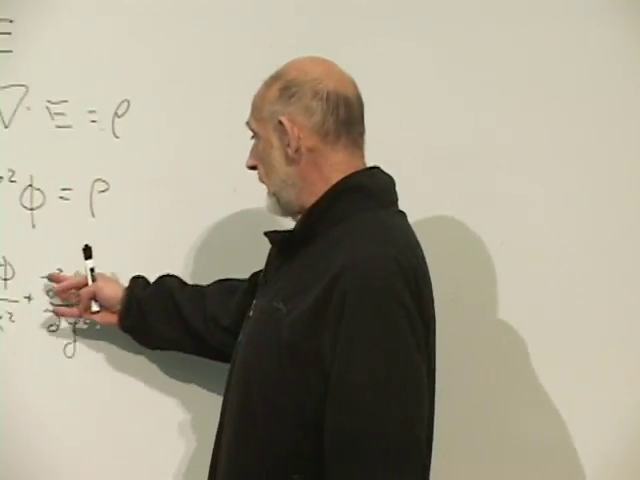
\includegraphics[width=0.70\textwidth]{lecture_08_figure_02.png}
  \caption{Cặp phương trình Cauchy--Riemann hoàn chỉnh, kể cả dấu trừ tương đối.}
  \lectureframe{00:19:48}
  \label{fig:l08-cr-board}
\end{figure}

Bài giảng phân biệt ngắn gọn các thuật ngữ liên quan. Một hàm chỉnh hình trên toàn bộ mặt phẳng phức hữu hạn là một hàm nguyên. Một hàm phân hình có thể có các cực cô lập. Vì vậy \(1/z\) là giải tích ở ngoài \(z=0\), nhưng nó không phải là hàm nguyên.

\section{Các hàm điều hòa liên hợp và hình học bảo giác}

Các phương trình Cauchy--Riemann là các phương trình bậc một ghép cặp, nhưng chúng kéo theo các phương trình bậc hai riêng rẽ. Lấy đạo hàm của
\(\partial_xu=\partial_yv\) theo \(x\), lấy đạo hàm của
\(\partial_yu=-\partial_xv\) theo \(y\), rồi cộng lại:
\begin{align}
  \partial_x^2u&=\partial_x\partial_yv,\\
  \partial_y^2u&=-\partial_y\partial_xv,\\
  \therefore\qquad
  \partial_x^2u+\partial_y^2u&=0.
  \label{eq:l08-harmonic-u}
\end{align}
Lặp lại lập luận với \(u\) và \(v\) hoán đổi cho nhau thì được
\begin{equation}
  \partial_x^2v+\partial_y^2v=0.
  \label{eq:l08-harmonic-v}
\end{equation}
Vì thế phần thực và phần ảo của một hàm giải tích là các hàm điều hòa liên hợp. Hai hàm điều hòa tùy ý không tự động tạo thành một hàm giải tích; chúng vẫn phải được liên hệ với nhau bởi
\eqref{eq:l08-cauchy-riemann}.

\begin{figure}[H]
  \centering
  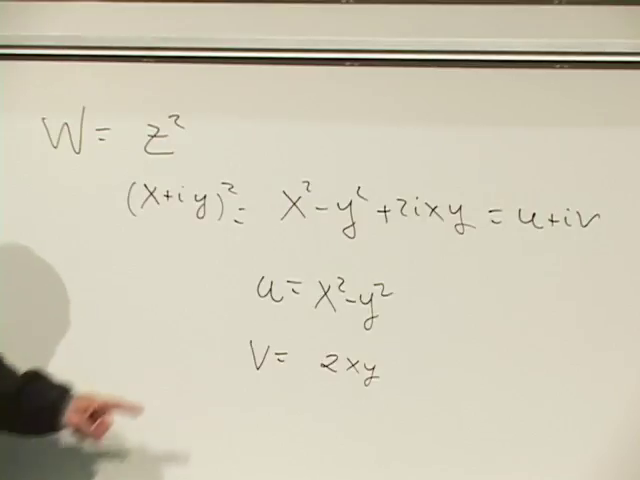
\includegraphics[width=0.68\textwidth]{lecture_08_figure_03.png}
  \caption{Các đạo hàm hỗn hợp triệt tiêu, để lại phương trình Laplace cho một thành phần của ánh xạ giải tích.}
  \lectureframe{00:23:09}
  \label{fig:l08-harmonic-board}
\end{figure}

Cũng có một cách diễn giải vectơ hữu ích. Nếu
\(\mathbf F=(u,-v)\), thì hai phương trình Cauchy--Riemann phát biểu, tùy theo quy ước định hướng đã chọn, rằng cả phân kỳ lẫn xoáy hai chiều của \(\mathbf F\) đều triệt tiêu. Đây là sự quay lại với tĩnh điện học đã được báo trước.

\subsection{Vì sao các góc được bảo toàn}

Viết hai độ dời phức nhỏ ở dạng cực:
\begin{equation}
  \delta z=\rho e^{i\theta},
  \qquad
  \Delta z=\rho'e^{i\theta'}.
\end{equation}
Tỉ số của chúng có pha \(\theta-\theta'\), đúng bằng góc giữa chúng.
Dưới một ánh xạ giải tích,
\begin{equation}
  \frac{\delta w}{\delta z}
  =\frac{\Delta w}{\Delta z}
  =w'(z),
\end{equation}
vì đạo hàm không phụ thuộc vào hướng. Sắp xếp lại cho
\begin{equation}
  \frac{\Delta z}{\delta z}
  =\frac{\Delta w}{\delta w}.
  \label{eq:l08-angle-ratio}
\end{equation}
Hai vế có cùng pha, nên góc giữa các độ dời ban đầu bằng góc giữa các ảnh của chúng.

\begin{figure}[H]
  \centering
  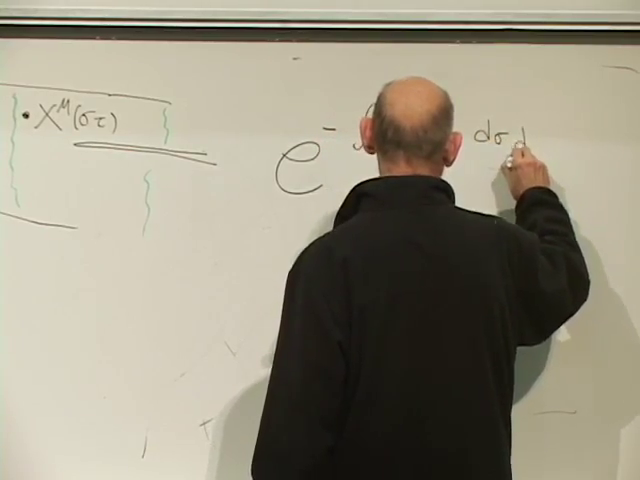
\includegraphics[width=0.70\textwidth]{lecture_08_figure_04.png}
  \medskip

  \begin{tikzpicture}[x=0.9cm,y=0.9cm,>=Latex]
    \begin{scope}
      \draw[->] (-0.2,0) -- (2.3,0);
      \draw[->] (0,-0.2) -- (0,2.1);
      \draw[very thick,blue!65!black,->] (0,0) -- (1.85,0.45)
        node[right] {\(\delta z\)};
      \draw[very thick,orange!75!black,->] (0,0) -- (0.72,1.65)
        node[above] {\(\Delta z\)};
      \draw (0.58,0.14) arc[start angle=14,end angle=66,radius=0.60];
      \node at (1.0,-0.55) {\(z\)-plane};
    \end{scope}
    \draw[->,thick] (3.0,0.9) -- (4.2,0.9)
      node[midway,above] {\(w(z)\)};
    \begin{scope}[xshift=5.0cm]
      \draw[->] (-0.2,0) -- (2.3,0);
      \draw[->] (0,-0.2) -- (0,2.1);
      \draw[very thick,blue!65!black,->] (0,0) -- (1.65,0.70)
        node[right] {\(\delta w\)};
      \draw[very thick,orange!75!black,->] (0,0) -- (0.48,1.62)
        node[above] {\(\Delta w\)};
      \draw (0.54,0.23) arc[start angle=23,end angle=74,radius=0.59];
      \node at (1.0,-0.55) {\(w\)-plane};
    \end{scope}
  \end{tikzpicture}
  \caption{Chứng minh trên bảng và một cách dựng lại cục bộ gọn gàng. Phép nhân với \(w'(z)\) quay và co giãn mọi hướng vi phân theo cùng một lượng, nhờ đó bảo toàn góc tương đối của chúng.}
  \lectureframe{00:34:11}
  \label{fig:l08-angle-proof}
\end{figure}

Lập luận cục bộ này giả sử \(w'(z)\neq0\). Tại một điểm tới hạn, ánh xạ có thể không còn là một-một theo địa phương, và khi đó phải xét riêng hình học. Tránh xa những điểm như vậy, các ánh xạ giải tích và các ánh xạ bảo giác bảo toàn định hướng là cùng một đối tượng xét theo địa phương.

\section{Những ví dụ để luyện mắt}

\subsection{Phép bình phương và liên hợp phức}

Với \(w=z^2\),
\begin{equation}
  (x+iy)^2=x^2-y^2+2ixy=u+iv,
\end{equation}
nên
\begin{equation}
  u=x^2-y^2,
  \qquad
  v=2xy.
  \label{eq:l08-z-squared-components}
\end{equation}
Các đạo hàm bậc hai của \(u\) là \(2\) và \(-2\); các đạo hàm bậc hai của \(v\) thì riêng rẽ đều triệt tiêu. Cả hai đều điều hòa, và việc vi phân trực tiếp cũng xác nhận các phương trình Cauchy--Riemann.

\begin{figure}[H]
  \centering
  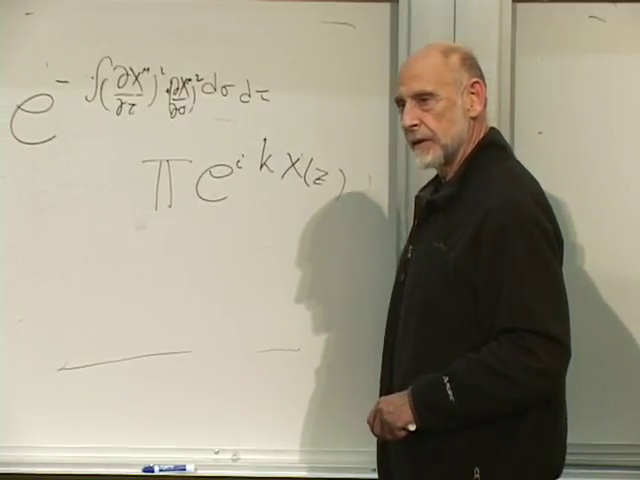
\includegraphics[width=0.72\textwidth]{lecture_08_figure_05.png}
  \caption{Ánh xạ bình phương được tách thành các thành phần điều hòa thực và ảo của nó.}
  \lectureframe{00:36:45}
  \label{fig:l08-z-square-board}
\end{figure}

\begin{classroomqa}
\audiencequestion{Liệu \(1/z\) có cho một ví dụ không giải tích không?
\lecturetimestamp{00:37:49}}
\lecturerresponse{Chỉ tại một điểm. Nó giải tích ở mọi nơi \(z\neq0\)
và có một cực tại gốc tọa độ. Muốn thấy một ánh xạ thất bại phép kiểm tra
Cauchy--Riemann ở mọi nơi, liên hợp phức là một ví dụ tốt hơn.}
\end{classroomqa}

Ngược lại,
\begin{equation}
  w=\bar z=x-iy
  \qquad\Longrightarrow\qquad
  u=x,\quad v=-y
\end{equation}
đảo ngược định hướng. Các đạo hàm của nó không thỏa phương trình
Cauchy--Riemann thứ nhất do sai khác dấu, nên nó không giải tích như một hàm của
\(z\).

\begin{figure}[H]
  \centering
  \includegraphics[width=0.62\textwidth]{lecture_08_figure_06.png}
  \caption{Liên hợp phức cung cấp một phản ví dụ cố ý không giải tích.}
  \lectureframe{00:38:38}
  \label{fig:l08-conjugate-board}
\end{figure}

\subsection{Hàm mũ và hàm nghịch đảo của nó}

\begin{classroomqa}
\audiencequestion{Nếu \(e^z\) là giải tích, vì sao hàm nghịch đảo của nó
\(\log z\) cũng phải giải tích? \lecturetimestamp{00:40:38}}
\lecturerresponse{Ở nơi hàm nghịch đảo tồn tại và \(w'(z)\neq0\), đạo hàm của nó là \(1/w'(z)\). Vì thế tính độc lập với hướng được bảo toàn. Trên toàn cục, logarit là đa trị, nên ta chọn một nhánh và loại trừ điểm phân nhánh cùng đường cắt của nó. Mệnh đề bảo giác cục bộ vẫn đúng trên miền đã chọn đó.}
\end{classroomqa}

Công thức Euler cho
\begin{equation}
  w=e^z=e^{x+iy}
  =e^x(\cos y+i\sin y),
\end{equation}
do đó
\begin{equation}
  u=e^x\cos y,
  \qquad
  v=e^x\sin y.
  \label{eq:l08-exponential-components}
\end{equation}
Chẳng hạn,
\(\partial_xu=e^x\cos y=\partial_yv\), và phương trình Cauchy--Riemann thứ hai cũng theo ra trực tiếp như vậy.

\begin{figure}[H]
  \centering
  \includegraphics[width=0.68\textwidth]{lecture_08_figure_07.png}
  \caption{Các thành phần thực và ảo của ánh xạ mũ.}
  \lectureframe{00:42:23}
  \label{fig:l08-exponential-board}
\end{figure}

\section{Nửa mặt phẳng, dải, hình trụ và đĩa}

\subsection{Logarit biến bán kính thành thời gian}

Xét nửa mặt phẳng phải, nơi
\(-\pi/2<\theta<\pi/2\), và viết
\begin{equation}
  z=re^{i\theta},
  \qquad
  w=\log z=\log r+i\theta.
  \label{eq:l08-log-map}
\end{equation}
Nửa mặt phẳng được ánh xạ thành dải vô hạn
\begin{equation}
  -\frac{\pi}{2}<\operatorname{Im}w<\frac{\pi}{2}.
\end{equation}
Các tia có \(\theta\) cố định trở thành các đường nằm ngang, còn các nửa đường tròn có \(r\) cố định trở thành các đường thẳng đứng. Gốc tọa độ được ánh xạ tới
\(\operatorname{Re}w=-\infty\), còn \(r=\infty\) tới
\(\operatorname{Re}w=+\infty\).

\begin{figure}[H]
  \centering
  \includegraphics[width=0.75\textwidth]{lecture_08_figure_08.png}
  \caption{Logarit biến nửa mặt phẳng phải thành một dải vô hạn: các tia cực và các nửa đường tròn trở thành một lưới chữ nhật trực giao.}
  \lectureframe{00:47:48}
  \label{fig:l08-log-strip-board}
\end{figure}

Dải là mặt thế giới chuẩn của một dây mở. Tọa độ bị chặn của nó là tham số dọc theo dây, còn phép tịnh tiến theo hướng không bị chặn tương ứng với thời gian mặt thế giới. Dưới ánh xạ mũ nghịch, một phép tịnh tiến theo thời gian trở thành một phép co giãn \(z\mapsto e^a z\). Vì vậy cùng một đối xứng trông như phép tịnh tiến trên dải và như sự dãn đều trên nửa mặt phẳng.

\begin{classroomqa}
\audiencequestion{Một giá trị cụ thể như \(r=1\) đi tới đâu, và các tọa độ trên dải có còn là tọa độ cực không? \lecturetimestamp{00:50:58}}
\lecturerresponse{Một đường tròn có bán kính cố định trở thành một đường thẳng đứng tại
\(\operatorname{Re}w=\log r\); riêng \(r=1\) được ánh xạ tới đường trung tâm
\(\operatorname{Re}w=0\). Tọa độ cực mô tả mặt phẳng
\(z\). Mặt phẳng \(w\) dùng các tọa độ chữ nhật thông thường
\((\log r,\theta)\).}
\end{classroomqa}

Nếu toàn bộ mặt phẳng bị đục lỗ được ánh xạ bởi \(\log z\), tọa độ góc có chu kỳ \(2\pi\). Vì vậy dải thu được có các cạnh trên và dưới được đồng nhất với nhau: nó là một hình trụ vô hạn. Nửa mặt phẳng có biên mô tả mặt thế giới của dây mở; toàn mặt phẳng, không có biên và có góc tuần hoàn, mô tả một hình trụ của dây kín.

\begin{figure}[H]
  \centering
  \includegraphics[width=0.75\textwidth]{lecture_08_figure_09.png}
  \caption{Bức tranh nửa mặt phẳng/dải và phép đồng nhất tuần hoàn biến toàn bộ mặt phẳng bị đục lỗ thành một hình trụ của dây kín.}
  \lectureframe{00:54:23}
  \label{fig:l08-open-closed-board}
\end{figure}

\subsection{Một ánh xạ Cayley tới đĩa đơn vị}

Một ánh xạ phân tuyến tính, hay Möbius, biến nửa mặt phẳng phải thành đĩa đơn vị:
\begin{equation}
  w=\frac{z-1}{z+1}.
  \label{eq:l08-cayley}
\end{equation}
Nó biến \(z=0\) thành \(-1\), \(z=\infty\) thành \(+1\), và trục ảo thành \(|w|=1\). Nếu \(z=ir\),
\begin{equation}
  \left|\frac{ir-1}{ir+1}\right|=1.
\end{equation}
Các điểm thỏa \(\operatorname{Re}z>0\) nằm bên trong đường tròn; nửa mặt phẳng trái được ánh xạ ra bên ngoài nó.
\editorialnote{Trong quá trình suy dẫn trực tiếp, nghịch đảo
\((z+1)/(z-1)\) được viết ra trong khi ảnh là miền trong của đĩa đang được mô tả.
Nghịch đảo đó có cùng biên là đường tròn đơn vị nhưng biến nửa mặt phẳng phải ra miền ngoài. Phương trình \eqref{eq:l08-cayley} là quy ước cho miền trong đĩa, nhất quán với hình học đã nêu.}

\begin{figure}[H]
  \centering
  \includegraphics[width=0.72\textwidth]{lecture_08_figure_10.png}
  \caption{Phép dựng biên đường tròn đơn vị bằng ánh xạ phân tuyến tính. Quy ước nghịch đảo nhìn thấy trên bảng hoán đổi miền trong và miền ngoài.}
  \lectureframe{00:58:38}
  \label{fig:l08-cayley-board}
\end{figure}

Ánh xạ Möbius biến họ suy rộng gồm các đường tròn và đường thẳng thành các đường tròn và đường thẳng. Vì thế lưới gồm các tia và các đường tròn trên nửa mặt phẳng trở thành hai họ cung trực giao trên đĩa. Một đường kính thẳng đơn giản là trường hợp giới hạn của một đường tròn có tâm đi ra vô cực.

\begin{classroomqa}
\audiencequestion{Các cung được vẽ bên trong đĩa có thực sự là các đường tròn không?
\lecturetimestamp{01:00:55}}
\lecturerresponse{Có. Tâm của chúng nằm ở các vị trí khác nhau, thường ở ngoài phần đĩa nhìn thấy. Đường kính là giới hạn bán kính vô hạn của cùng họ đó.}
\end{classroomqa}

\begin{classroomqa}
\audiencequestion{Hình vẽ đĩa này có nghĩa là đó là một mặt cầu không, và nửa mặt phẳng còn lại đi đâu? \lecturetimestamp{01:01:21}}
\lecturerresponse{Hình vẽ ở đây là một đĩa phẳng, không phải mặt cầu. Nửa mặt phẳng phải được ánh xạ vào bên trong biên của nó, còn nửa mặt phẳng trái được ánh xạ ra bên ngoài. Nếu thêm điểm ở vô cực vào toàn bộ mặt phẳng phức, thì mặt phẳng mở rộng đó có thể được biểu diễn như một mặt cầu bằng phép chiếu lập thể; đó là một phát biểu toàn cục khác.}
\end{classroomqa}

\begin{classroomqa}
\audiencequestion{Những đường cong nào trên đĩa tương ứng với các tia xuyên tâm ban đầu và các nửa đường tròn bán kính không đổi? \lecturetimestamp{01:02:59}}
\lecturerresponse{Trục thực dương trở thành đường kính nối \(-1\) và \(+1\). Các tia khác trở thành những cung tròn nối cùng hai điểm biên đó. Các nửa đường tròn có bán kính cố định trở thành họ trực giao bắt đầu và kết thúc trên đường tròn đơn vị.}
\end{classroomqa}

\begin{figure}[H]
  \centering
  \includegraphics[width=0.72\textwidth]{lecture_08_figure_11.png}
  \caption{Các đường thẳng và nửa đường tròn trong nửa mặt phẳng trở thành các họ đường tròn và đường thẳng trực giao trong đĩa.}
  \lectureframe{01:03:48}
  \label{fig:l08-circle-grid-board}
\end{figure}

\section{Mặt thế giới của bốn dây}

Giờ ta có thể quay lại tán xạ. Hai dây mở đi vào, nhập lại thành một dây, truyền trong một khoảng thời gian tùy ý, rồi tách thành hai dây đi ra. Trong tọa độ dải, mặt thế giới trông như một dải ruy băng dài bị xẻ từ mỗi đầu---hình “băng quấn thể thao”. Thời gian sống trung gian không được chọn trước. Nó là một trong những lịch sử mà biên độ được tích phân trên đó.

Gọi \((\sigma,\tau)\) là các tọa độ trên mặt thế giới và để
\begin{equation}
  X^\mu=X^\mu(\sigma,\tau)
  \label{eq:l08-embedding}
\end{equation}
cho biết vị trí của nó trong không-thời gian. Các nhãn \(\sigma,\tau\) nằm trên mặt tham số hai chiều; chỉ số \(\mu\) gắn nhãn các tọa độ không-thời gian. Trong lý thuyết boson \(\mu=0,\ldots,25\); trong trường hợp siêu dây có mười tọa độ không-thời gian.

Sau phép quay Wick, các trường nhúng tự do có tác dụng Euclid
\begin{equation}
  S_E[X]
  =\frac{1}{4\pi\alpha'}\int_\Sigma d\sigma\,d\tau\,
  \left[
    \partial_\tau X^\mu\partial_\tau X_\mu
    +\partial_\sigma X^\mu\partial_\sigma X_\mu
  \right].
  \label{eq:l08-euclidean-action}
\end{equation}
Tích phân đường đi tương ứng lấy tổng trên mọi phép nhúng của mặt thế giới đã chọn vào không-thời gian:
\begin{equation}
  \int\mathcal D X\,e^{-S_E[X]}.
  \label{eq:l08-bare-worldsheet-integral}
\end{equation}

\begin{figure}[H]
  \centering
  \includegraphics[width=0.74\textwidth]{lecture_08_figure_12.png}
  \caption{Trọng số Euclid dương hoàn chỉnh của mặt thế giới. Hai hạng đạo hàm được cộng trên mọi thành phần không-thời gian.}
  \lectureframe{01:11:34}
  \label{fig:l08-action-board}
\end{figure}

Dải bị xẻ có một biên liên thông. Vì vậy, tự do bảo giác cho phép biểu diễn nó như một đĩa. Bốn đầu ở xa của các dải trở thành bốn điểm được đánh dấu trên biên. Việc biến dạng các điểm đánh dấu làm thay đổi độ tách biểu kiến giữa chỗ ghép và chỗ tách trong tọa độ dải, nhưng không làm thay đổi mặt cơ sở hay vật lý.

\begin{figure}[H]
  \centering
  \includegraphics[width=0.76\textwidth]{lecture_08_figure_13.png}
  \caption{Mặt thế giới dạng dải bị xẻ và biểu diễn của nó bằng đĩa với các điểm biên ứng với các dây ngoài.}
  \lectureframe{01:15:18}
  \label{fig:l08-bandage-disc-board}
\end{figure}

Những đường lưới chi tiết dùng để minh họa phép ánh xạ bảo giác này không mang nội dung vật lý nào. Điều quan trọng là tôpô, biên và các điểm được đánh dấu ứng với các trạng thái ngoài. Cùng một mặt thế giới có thể được kéo dãn thành những hình biểu diễn kênh khác nhau mà không đưa vào một tương tác mới.

\section{Các trạng thái ngoài dưới dạng các phép chèn trên biên}

Tích phân trần \eqref{eq:l08-bare-worldsheet-integral} vẫn chưa cho biết những xung lượng nào đi vào và đi ra. Đối với một trạng thái dây mở vô hướng có xung lượng \(k_i^\mu\), hãy chèn trên biên toán tử đỉnh
\begin{equation}
  V_i(z_i)=e^{\,i k_i\cdot X(z_i)},
  \qquad
  k_i\cdot X=k_{i\mu}X^\mu.
  \label{eq:l08-vertex}
\end{equation}
Điểm \(z_i\) là một vị trí trên biên của mặt thế giới. Nó không phải là một tọa độ không-thời gian và cũng không phải là một hướng của xung lượng.

\begin{figure}[H]
  \centering
  \includegraphics[width=0.72\textwidth]{lecture_08_figure_14.png}
  \caption{Trọng số Euclid của phần trong và tích các phép chèn xung lượng trên biên được hiển thị như những thừa số tách biệt.}
  \lectureframe{01:18:58}
  \label{fig:l08-vertex-board}
\end{figure}

Đối với \(n\) dây mở ngoài, quy tắc dạng sơ đồ là
\begin{equation}
  \begin{aligned}
    \mathcal A_n(k_1,\ldots,k_n)
    &=\int_{\mathcal M_{0,n}^{\partial}}\!d\mu(z_i)
      \int\mathcal D X\\
    &\quad\times e^{-S_E[X]}
      \prod_{i=1}^{n}e^{\,i k_i\cdot X(z_i)}.
  \end{aligned}
  \label{eq:l08-open-string-prescription}
\end{equation}
Tích phân hàm được lấy trên các phép nhúng \(X^\mu\). Tích phân hữu hạn chiều được lấy trên các vị trí chèn trên biên không tương đương. Ở giai đoạn này, các thừa số phân cực và độ đo cố định chuẩn được lược bỏ, đúng như trong bài giảng.
\editorialnote{Một biên độ dây hoàn chỉnh sau khi cố định chuẩn còn chứa đóng góp ghost thích hợp, các thừa số đỉnh phụ thuộc trạng thái, các hằng số liên kết và chuẩn hóa. Phương trình
\eqref{eq:l08-open-string-prescription} ghi lại sự phụ thuộc vào trường nhúng và vị trí được phát triển trong bài giảng này.}

\begin{classroomqa}
\audiencequestion{Nếu các xung lượng ngoài đã cố định, vì sao lại lấy tích phân trên chúng? \lecturetimestamp{01:20:42}}
\lecturerresponse{Không phải vậy. Các \(k_i\) là những nhãn cố định của biên độ tán xạ. Cái được tích phân là các trường nhúng và các vị trí trên mặt thế giới \(z_i\) tại đó những xung lượng cố định ấy được chèn vào. Tích phân sau thay thế tích phân trên thời gian sống trung gian trong hình dải.}
\end{classroomqa}

\begin{classroomqa}
\audiencequestion{Liệu tích các thừa số đỉnh có nằm bên trong tích phân đường đi không, và nó có phải là một phần của tác dụng không? \lecturetimestamp{01:21:39}}
\lecturerresponse{Nó nhân với \(e^{-S_E}\) bên trong tích phân hàm. Một cách tương đương, ta có thể đưa các thừa số đó vào số mũ và xem chúng như các hạng nguồn cục bộ được cộng vào tác dụng, nhưng về mặt khái niệm chúng là các toán tử đỉnh chứ không phải là một phần của tác dụng tự do trong phần trong.}
\end{classroomqa}

\begin{figure}[H]
  \centering
  \includegraphics[width=0.76\textwidth]{lecture_08_figure_15.png}
  \caption{Tích phân đường đi được viết với các thừa số riêng rẽ
  \(e^{ik_i\cdot X(z_i)}\) cho các hạt ngoài lần lượt.}
  \lectureframe{01:23:23}
  \label{fig:l08-full-prescription-board}
\end{figure}

\begin{classroomqa}
\audiencequestion{Tại sao \(e^{ik\cdot X}\) vẫn còn chứa \(i\) sau phép quay Wick của mặt thế giới? \lecturetimestamp{01:23:42}}
\lecturerresponse{Phép quay làm thay đổi thời gian trên mặt thế giới và biến trọng số của phần trong từ \(e^{iS}\) thành \(e^{-S_E}\). \(i\) trong một hàm riêng xung lượng là pha Fourier gắn nhãn xung lượng không-thời gian. Nó có vai trò khác nên vẫn còn đó.}
\end{classroomqa}

\begin{classroomqa}
\audiencequestion{Liệu vị trí \(z_i\) có quyết định hướng của vectơ xung lượng không? \lecturetimestamp{01:24:19}}
\lecturerresponse{Không. Hướng được mã hóa trong các thành phần không-thời gian \(k_i^\mu\). Điểm chèn \(z_i\) cho biết xung lượng đó đi vào mô tả mặt thế giới ở đâu; \(X^\mu(z_i)\) là một trong những giá trị trường được lấy tổng trong \(\mathcal D X\).}
\end{classroomqa}

\begin{classroomqa}
\audiencequestion{Liệu các góc được vẽ của các nhánh băng quấn có mã hóa các hướng của những xung lượng vật lý không? \lecturetimestamp{01:25:07}}
\lecturerresponse{Không. Hình băng quấn là không gian tham số, không phải là ảnh của dây trong không-thời gian vật lý. Các nhánh của nó có thể được vẽ nằm ngang, nghiêng, hoặc uốn theo phép bảo giác. Các hướng vật lý được mang bởi các thành phần \(k^\mu\), còn \(X^\mu(\sigma,\tau)\) thì được tích phân.}
\end{classroomqa}

\section{Tích phân Gauss như tĩnh điện học}

Tác dụng \eqref{eq:l08-euclidean-action} là bậc hai theo từng thành phần \(X^\mu\), và các phép chèn trở thành những nguồn tuyến tính một khi các hàm mũ của chúng được gộp với tác dụng. Vì vậy tích phân hàm là Gauss. Tại điểm yên ngựa của nó, mỗi thành phần không-thời gian thỏa mãn một phương trình Poisson có dạng sơ đồ
\begin{equation}
  \nabla^2 X^\mu(z)
  \propto
  i\alpha'\sum_i k_i^\mu\,\delta(z-z_i),
  \label{eq:l08-electrostatic-source}
\end{equation}
kèm điều kiện biên của dây mở trên vành đĩa. Mỗi \(X^\mu\) hành xử như một thế tĩnh điện độc lập, và mỗi thành phần xung lượng \(k_i^\mu\) hành xử như điện tích tương ứng đặt tại \(z_i\).

\begin{figure}[H]
  \centering
  \includegraphics[width=0.76\textwidth]{lecture_08_figure_16.png}
  \caption{Đĩa với các nguồn trên biên được diễn giải như một bài toán tĩnh điện hai chiều độc lập cho mỗi thành phần không-thời gian.}
  \lectureframe{01:28:58}
  \label{fig:l08-electrostatic-disc-board}
\end{figure}

Giải bài toán tĩnh điện, tính năng lượng của nó, lấy mũ của âm năng lượng đó, và cuối cùng tích phân trên các vị trí điện tích không tương đương. Trong chuẩn hóa dây mở tiêu chuẩn, hàm tương quan của trường nhúng cung cấp thừa số Koba--Nielsen
\begin{equation}
  \left\langle\prod_i e^{\,ik_i\cdot X(z_i)}\right\rangle
  \propto
  (2\pi)^D\delta^{(D)}\!\left(\sum_i k_i\right)
  \prod_{i<j}|z_i-z_j|^{2\alpha' k_i\cdot k_j}.
  \label{eq:l08-koba-nielsen}
\end{equation}
Hàm delta biểu thị bảo toàn xung lượng. Tích đó chứa các năng lượng cặp tĩnh điện. Đối với bốn phép chèn biên vô hướng được dùng ở đây, việc cố định ba vị trí biến tích phân còn lại thành tích phân beta Euler đã gặp trong các bài giảng trước.

\begin{classroomqa}
\audiencequestion{Có hai mươi sáu năng lượng tĩnh điện hay chỉ một?
\lecturetimestamp{01:30:53}}
\lecturerresponse{Có một thế và trường độc lập cho mỗi thành phần không-thời gian. Các năng lượng bậc hai của chúng không có hạng chéo trong một cơ sở trực chuẩn của không gian đích, và các đóng góp được cộng vào một tác dụng tổng cộng duy nhất trước khi lấy mũ.}
\end{classroomqa}

\begin{classroomqa}
\audiencequestion{Liệu tọa độ góc của đĩa có phải là góc tán xạ vật lý không? \lecturetimestamp{01:32:10}}
\lecturerresponse{Không. Nó là một tham số vị trí trên mặt thế giới. Tổ hợp không tương đương của nó liên hệ với khoảng truyền trung gian và được tích phân. Góc tán xạ vật lý được mã hóa thông qua các bất biến Lorentz xây dựng từ các xung lượng cố định.}
\end{classroomqa}

\begin{classroomqa}
\audiencequestion{Tại sao phép dựng này thất bại khi rời khỏi số chiều tới hạn? \lecturetimestamp{01:32:35}}
\lecturerresponse{Chỉ riêng các tích phân Gauss hình thức chưa phải toàn bộ điều kiện nhất quán. Việc cố định chuẩn đưa vào một bất thường bảo giác mà các đóng góp vật chất và ghost của nó chỉ triệt tiêu tại số chiều tới hạn: \(D=26\) đối với dây boson và \(D=10\) đối với siêu dây. Không có sự triệt tiêu đó, đối xứng bảo giác được giả định của mặt thế giới lượng tử sẽ mất đi.}
\end{classroomqa}

\begin{classroomqa}
\audiencequestion{Chúng ta đã giả thiết ba chiều không gian lớn và các chiều phụ compact chưa? \lecturetimestamp{01:33:38}}
\lecturerresponse{Chưa. Compact hóa vẫn chưa đi vào phép dựng này. Ở giai đoạn này, các tọa độ boson vẫn còn chạy trên cả hai mươi sáu hướng của không gian đích, hoặc mười trong trường hợp siêu dây. Việc một tập con trong số đó có thể vẫn lớn ở thang vĩ mô như thế nào là chủ đề của phần thảo luận tiếp theo.}
\end{classroomqa}

\begin{classroomqa}
\audiencequestion{Liệu mối liên hệ với tĩnh điện học chỉ đơn giản là các tọa độ thỏa mãn phương trình Laplace? \lecturetimestamp{01:33:57}}
\lecturerresponse{Chính xác. Xa các điểm chèn, mỗi \(X^\mu\) là điều hòa; các toán tử đỉnh cung cấp các nguồn hàm delta. Về mặt toán học, đó chính là cùng bài toán giá trị biên như đối với một thế tĩnh hai chiều có các điện tích điểm, bất kể ta có dùng ngôn ngữ tĩnh điện hay không.}
\end{classroomqa}

\subsection{Tính dư thừa bảo giác và số môđun}

Đĩa có nhóm tự đẳng cấu bảo giác 3 tham số thực,
\(\mathrm{PSL}(2,\mathbb R)\). Vì vậy, có thể cố định ba điểm biên có thứ tự tại những vị trí thuận tiện. Đối với bốn dây ngoài, chỉ còn vị trí thứ tư cần được tích phân; đối với \(n\) phép chèn biên có thứ tự thì có
\begin{equation}
  n-3
  \label{eq:l08-n-minus-three}
\end{equation}
tích phân vị trí thực ở mức cây.

\begin{classroomqa}
\audiencequestion{Có bốn vị trí góc độc lập quanh đĩa không? \lecturetimestamp{01:34:37}}
\lecturerresponse{Không phải về mặt vật lý. Ban đầu ta viết bốn vị trí, nhưng đối xứng bảo giác của đĩa có thể đặt bất kỳ ba vị trí nào ở chỗ thuận tiện. Đối với biên độ hai-vào/hai-ra, chỉ còn vị trí tương đối của điểm thứ tư.}
\end{classroomqa}

\begin{figure}[H]
  \centering
  \includegraphics[width=0.72\textwidth]{lecture_08_figure_17.png}
  \caption{Bốn phép chèn trên biên của đĩa. Tự do bảo giác cho phép cố định bất kỳ ba điểm nào, để lại một môđun bốn điểm.}
  \lectureframe{01:35:18}
  \label{fig:l08-fix-three-board}
\end{figure}

\begin{classroomqa}
\audiencequestion{Nếu hai điểm tách không xuất hiện ở cùng một độ cao trong hình vẽ dải thì sao? \lecturetimestamp{01:35:24}}
\lecturerresponse{Một ánh xạ bảo giác có thể dời đi sự lệch biểu kiến đó. Những hình vẽ khác nhau là các biểu diễn tọa độ của cùng một môđun. Tích phân bất biến là tích phân trên vị trí biên còn lại, tương đương với tích phân trên khoảng truyền.}
\end{classroomqa}

\begin{classroomqa}
\audiencequestion{Với nhiều hạt ngoài hơn, còn lại bao nhiêu tham số vị trí? \lecturetimestamp{01:36:00}}
\lecturerresponse{Cố định ba điểm chèn bằng đối xứng bảo giác và tích phân các điểm \(n-3\) còn lại. Đây là số đếm môđun biên cho một biên độ dây mở có thứ tự ở mức cây.}
\end{classroomqa}

\begin{classroomqa}
\audiencequestion{Điều này liên hệ thế nào với M-lý thuyết?
\lecturetimestamp{01:36:37}}
\lecturerresponse{Chưa. Phép dựng ở đây là tán xạ dây mở nhiễu loạn trên một mặt thế giới. Mối liên hệ của nó với M-lý thuyết đòi hỏi các ý tưởng đối ngẫu và phi nhiễu loạn về sau, nên câu hỏi này được hoãn lại một cách tường minh.}
\end{classroomqa}

\begin{classroomqa}
\audiencequestion{Một cách biểu diễn bằng dải thẳng đứng hoặc dải chéo khác có phải là một phép tính khác không? \lecturetimestamp{01:36:49}}
\lecturerresponse{Không. Ta có thể giữ cố định một điểm thuận tiện và để môđun còn lại chạy qua toàn bộ khoảng của nó. Các hình dải và tích phân theo điểm biên trên đĩa là những cách cắt khác nhau của cùng một tích phân, đó là lý do vì sao có thể xử lý đối xứng mọi dây ngoài.}
\end{classroomqa}

\section{Những điều mà quy tắc này vẫn chưa giải quyết}

Công thức trên đĩa mở rộng ngay lập tức sang nhiều dây ngoài hơn: thêm nhiều toán tử đỉnh hơn và lấy tích phân theo \(n-3\) vị trí biên không tương đương của chúng. Đây là một quy tắc ở mức cây chính xác cho một mô hình dây nhất quán, nhưng nó vẫn chưa phải là một mô hình hiện thực của vật lý hạt đã được quan sát. Lý thuyết boson đơn giản có số chiều không-thời gian sai và còn có thêm những khiếm khuyết vật lý khác. Siêu dây cải thiện phổ và hạ số chiều tới hạn xuống mười, nhưng sáu chiều không gian vẫn phải được compact hóa.

\begin{classroomqa}
\audiencequestion{Mô hình đơn giản này đã phù hợp với các thí nghiệm va chạm hạt chưa? \lecturetimestamp{01:39:06}}
\lecturerresponse{Không. Về mặt lịch sử, cấu trúc cộng hưởng của nó giống tán xạ hadron, nhưng mô hình boson hai mươi sáu chiều không thể là một mô tả trực tiếp về các hạt đã được quan sát. Hình thức luận này xác định các biên độ tán xạ cho mô hình; để khớp với tự nhiên còn cần một phổ hiện thực, sự compact hóa, các tương tác và việc chọn chân không.}
\end{classroomqa}

\begin{classroomqa}
\audiencequestion{Liệu compact hóa có làm giảm các chiều dư và cho ra dữ liệu hạt phù hợp thực tế không? \lecturetimestamp{01:41:10}}
\lecturerresponse{Nó có thể làm giảm số chiều vĩ mô hiệu dụng và sinh ra các phổ hạt cùng các nhóm chuẩn. Đây cũng là nơi phần lớn khó khăn toán học thực sự xuất hiện. Nhiều compact hóa nhất quán đã được biết đến, và việc chọn ra một mô hình duy nhất của các hạt cơ bản đã được quan sát vẫn chưa được giải quyết.}
\end{classroomqa}

Bài giảng nhấn mạnh sự phân biệt này thay vì quảng bá một lý thuyết đã hoàn chỉnh. Các cách xây dựng của lý thuyết dây được xác định rõ ràng về mặt toán học và đã đem lại những hiểu biết sâu sắc về hấp dẫn và hình học, nhưng chính sự đa dạng của chúng lại là một phần của bài toán vật lý.

\begin{classroomqa}
\audiencequestion{Có cách ngắn gọn nào để nhớ vì sao số chiều tới hạn của lý thuyết boson là hai mươi sáu không? \lecturetimestamp{01:43:19}}
\lecturerresponse{Phép tính dao động tử trước đó đã dùng tổng không điểm được chính quy hóa \(1+2+3+\cdots=-1/12\). Phần đóng góp của dao động tử ngang liên quan đến 24 phương, và khi khôi phục 2 tọa độ không-thời gian dọc thì ta được \(24+2=26\). Đây là một mẹo ghi nhớ cho lập luận nhất quán trước đó, chứ không phải là một phép suy ra mới ở đây.}
\end{classroomqa}

\begin{classroomqa}
\audiencequestion{Bản thân các xung lượng \(k_i\) được chèn vào có được lượng tử hóa không? \lecturetimestamp{01:43:46}}
\lecturerresponse{Trong không-thời gian không compact, các thành phần của chúng là liên tục. Đại lượng được lượng tử hóa là mức dao động tử, và do đó là phổ bình phương khối lượng được phép. Các chiều compact có thể lượng tử hóa các thành phần xung lượng và thành phần quấn tương ứng, nhưng điều đó thuộc về phần thảo luận tiếp theo.}
\end{classroomqa}
\chapter{Dây, hấp dẫn, compact hóa và đối ngẫu T}

\lectureoverview{Một hạt điểm có thể chuyển động nhất quán trên hầu như mọi hình học trơn, nhưng một dây lượng tử thì không thể. Vô số dao động điểm không của nó thăm dò không gian đích ở những thang độ ngày càng ngắn hơn, và hình học hiệu dụng thay đổi khi những dao động ấy được khôi phục. Đòi hỏi quá trình này có một điểm bất động suy ra \(R_{\mu\nu}=0\), phương trình Einstein chân không. Sau đó ta chuyển từ điều kiện nhất quán này sang compact hóa. Một đường tròn cung cấp cả các trạng thái xung lượng Kaluza--Klein lẫn các trạng thái quấn của dây; việc hoán đổi chúng đồng nhất một đường tròn bán kính \(R\) với một đường tròn bán kính \(\alpha'/R\).}

\section{Tính nhất quán như một nguyên lý tuyển chọn}

Có hai câu hỏi cần trả lời. Vì sao hấp dẫn xuất hiện trong lý thuyết dây, và vì sao lý thuyết dây kém dễ dãi hơn rất nhiều so với cơ học hạt điểm? Thực ra chúng chỉ là một câu hỏi. Một hình học nền chỉ được chấp nhận nếu dây có thể lan truyền trên đó mà không giữ lại sự phụ thuộc tùy tiện vào mức độ tinh mà ta phân giải dây.

Hãy bắt đầu với bài toán đối chứng: một hạt điểm bị ràng buộc trên một mặt cong trơn. Về mặt cổ điển, nó đi theo một đường trắc địa, tương tự nội tại của một đường thẳng. Ta có thể xấp xỉ chuyển động bằng nhiều đoạn ngắn, viết một phương trình sai phân, rồi cho độ dài đoạn tiến về 0. Kết quả là một phương trình vi phân thường với giới hạn liên tục được xác định rõ.

Cơ học lượng tử thay đổi phép tổng trên các lịch sử, chứ không thay đổi kết luận. Thay vì chọn một quỹ đạo cổ điển, ta cộng các biên độ trên những quỹ đạo nằm trên mặt đó. Thời gian lại có thể được chia thành các bước nhỏ, và giới hạn tương đương được mô tả bằng một phương trình Schr\"odinger trên không gian cấu hình cong. Đối với một mặt trơn, giới hạn hội tụ về một hàm truyền và một phổ xác định.

\begin{figure}[H]
  \centering
  \includegraphics[width=0.72\textwidth]{lecture_09_figure_01.png}
  \caption{Một đường đi trơn trên mặt và một đường gấp khúc từ phép tổng lượng tử chia lát theo thời gian. Cả hai đều vẫn là những đường nội tại trên mặt đích.}
  \lectureframe{00:05:10}
  \label{fig:l09-particle-paths}
\end{figure}

\begin{classroomqa}
\audiencequestion{Trong tích phân đường, có phải mọi quỹ đạo đều buộc phải ở trên mặt đó không? \lecturetimestamp{00:05:39}}
\lecturerresponse{Có. Mặt đó là không gian cấu hình của hạt, chứ không phải một tấm được nhúng trong một căn phòng lớn hơn để hạt có thể đi đường tắt xuyên qua. Mọi điểm trung gian đều thuộc về mặt đó, và mọi độ dài cũng như hàm tác dụng đều được tính bằng metric nội tại của nó.}
\end{classroomqa}

Câu hỏi tương ứng cho dây thì khó hơn. Một dây không chỉ được xác định bởi vị trí khối tâm. Nó mang một tháp vô hạn các dao động tử, nên việc tăng độ phân giải có nghĩa là cho phép nhiều bậc tự do động lực hơn. Lý thuyết chỉ nhất quán nếu các quan sát lượng tiến tới một giới hạn khi tháp ấy được khôi phục.

\section{Hạt điểm trên mặt cầu}

Mặt cầu là hình học kiểm tra cong đơn giản nhất. Gọi bán kính của nó là \(R\), và trước hết đặt lên đó một hạt khối lượng \(m\). Đối với chuyển động dọc theo một đại vòng,
\begin{equation}
  E=\frac{1}{2}mv^2=\frac{p^2}{2m},
  \qquad
  L=pR.
  \label{eq:l09-particle-energy}
\end{equation}
Do đó,
\begin{equation}
  E=\frac{L^2}{2mR^2}
   =\frac{L^2}{2I},
  \qquad
  I=mR^2.
  \label{eq:l09-rotor-energy}
\end{equation}
Bán kính đi vào qua mômen quán tính. Lượng tử hóa mômen động lượng góc cho phổ rôto cứng quen thuộc, và không có gì phụ thuộc vào một ngưỡng cắt tử ngoại.

\begin{figure}[H]
  \centering
  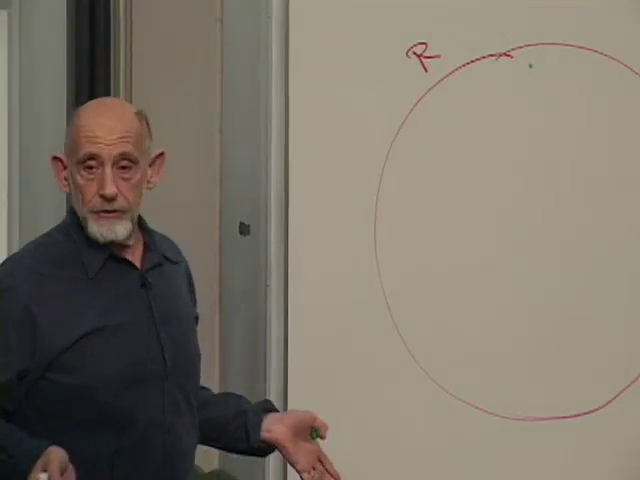
\includegraphics[width=0.74\textwidth]{lecture_09_figure_02.png}
  \caption{Phép tính đối chứng cho hạt điểm:
  \(p^2/(2m)=L^2/(2mR^2)=L^2/(2I)\).}
  \lectureframe{00:11:25}
  \label{fig:l09-sphere-rotor}
\end{figure}

Ví dụ không hề rắc rối này rất quan trọng. Bản thân độ cong không phải là vấn đề. Vấn đề xuất hiện khi độ cong ghép với độ trải rộng lượng tử nội tại của dây.

\section{Dây chân không không có dạng điểm}

Xét một tọa độ ngang của một dây mở và trừ đi tọa độ khối tâm của nó. Khai triển theo dao động tử dùng ở đây chỉ có tính sơ đồ:
\begin{equation}
  X(\sigma)-X_{\mathrm{cm}}
  \sim
  \sum_{n=1}^{\infty}
  \frac{a_n+a_n^\dagger}{\sqrt n}\cos(n\sigma).
  \label{eq:l09-mode-expansion}
\end{equation}
Các thành phần cốt yếu là các mode cosin, các toán tử dao động tử và thừa số \(1/\sqrt n\). Các chuẩn hóa chính xác không đóng vai trò nào trong lập luận về kích thước.
\editorialnote{Khai triển chính xác chứa các thừa số của \(\alpha'\) phụ thuộc vào quy ước, các hằng số số học và một lựa chọn ký hiệu dao động tử. Phương trình \eqref{eq:l09-mode-expansion} chỉ giữ lại sự phụ thuộc cần thiết cho ước lượng tử ngoại, đúng như trong phép suy dẫn trên bảng.}

\begin{figure}[H]
  \centering
  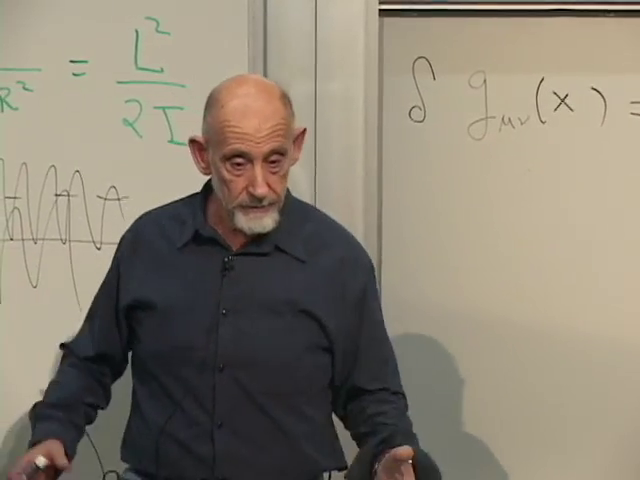
\includegraphics[width=0.78\textwidth]{lecture_09_figure_03.png}
  \caption{Khai triển dao động tử về mặt cấu trúc và tổng kép thu được khi bình phương nó.}
  \lectureframe{00:15:20}
  \label{fig:l09-string-modes}
\end{figure}

Bình phương khoảng cách tới khối tâm trong chân không của các dao động tử là
\begin{align}
  \expect{\bigl(X(\sigma)-X_{\mathrm{cm}}\bigr)^2}_0
  &\sim
  \sum_{n,m\geq1}
  \frac{\cos(n\sigma)\cos(m\sigma)}{\sqrt{nm}}\notag\\
  &\qquad\times
  \bra{0}(a_n+a_n^\dagger)\notag\\
  &\hspace{6em}\times(a_m+a_m^\dagger)\ket{0}.
  \label{eq:l09-size-double-sum}
\end{align}
Phần lớn các hạng đều triệt tiêu. Hai toán tử hủy triệt tiêu ket; hai toán tử tạo để lại một trạng thái trực giao với bra; và một toán tử tạo theo sau bởi một toán tử hủy cũng có giá trị kỳ vọng chân không bằng 0 trong thứ tự này. Phép co còn lại là
\begin{equation}
  \bra{0}a_n a_m^\dagger\ket{0}=\delta_{nm}.
  \label{eq:l09-vacuum-contraction}
\end{equation}

\begin{figure}[H]
  \centering
  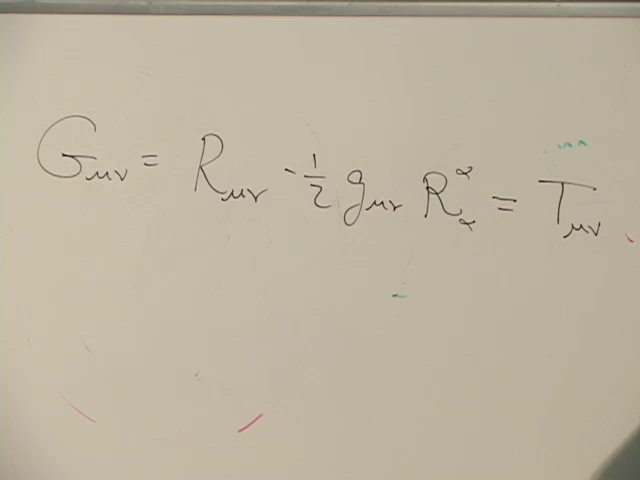
\includegraphics[width=0.74\textwidth]{lecture_09_figure_04.png}
  \caption{Phép co chân không còn lại rút tổng dao động tử kép về một tổng đơn.}
  \lectureframe{00:20:10}
  \label{fig:l09-vacuum-contraction}
\end{figure}

Do đó
\begin{equation}
  \expect{\bigl(X(\sigma)-X_{\mathrm{cm}}\bigr)^2}_0
  \sim
  \sum_{n=1}^{\infty}\frac{\cos^2(n\sigma)}{n}.
  \label{eq:l09-size-single-sum}
\end{equation}
Tại một điểm điển hình dọc theo dây, hoặc sau khi lấy trung bình theo \(\sigma\), \(\cos^2(n\sigma)\) đóng góp xấp xỉ \(1/2\). Với một ngưỡng cắt mode \(N\),
\begin{equation}
  \expect{\bigl(X-X_{\mathrm{cm}}\bigr)^2}_{0,N}
  \sim
  \frac{1}{2}\sum_{n=1}^{N}\frac{1}{n}
  =\frac{1}{2}\log N+O(1).
  \label{eq:l09-logarithmic-size}
\end{equation}

\begin{figure}[H]
  \centering
  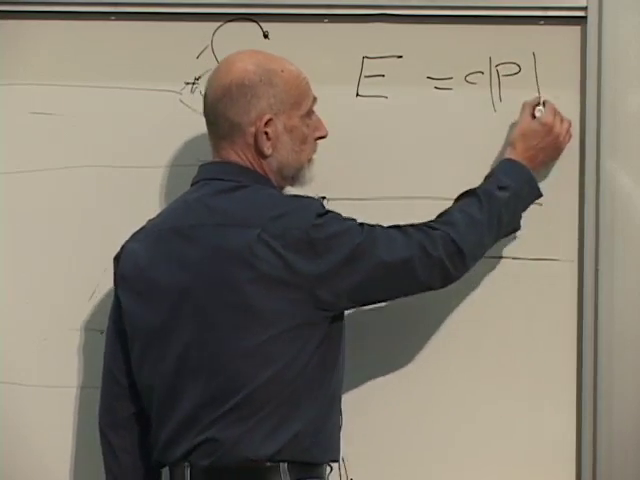
\includegraphics[width=0.72\textwidth]{lecture_09_figure_05.png}
  \caption{Trên bảng, ta đi đến tổng điều hòa chi phối độ trải rộng của trạng thái cơ bản.}
  \lectureframe{00:22:05}
  \label{fig:l09-harmonic-size}
\end{figure}

Chẳng hạn, nếu chỉ giữ 25 mode đầu tiên thì ta được một đối tượng mờ nhòe hữu hạn, nhưng đó vẫn chưa phải là dây trong giới hạn liên tục. Bỏ ngưỡng cắt đi làm cho độ trải rộng bình phương trung bình tăng theo logarit. Không nên hiểu nhầm kết luận này như một chứng minh rằng lý thuyết dây trong không gian phẳng là không nhất quán. Trong không gian phẳng, chuyển động của khối tâm và của các dao động tử tách rời nhau, và những sự triệt tiêu tinh tế trong các biên độ vật lý duy trì tính địa phương như kỳ vọng. Kích thước tăng dần là một lời cảnh báo. Độ cong cho ta biết liệu lời cảnh báo ấy có trở thành một thất bại hay không.

\section{Khi độ trải rộng nội tại làm thay đổi hình học}

Đặt dây gần cực bắc của mặt cầu. Khi mọi dao động tử đều bị tắt, nó ứng xử như hạt điểm vừa khảo sát. Khi cho phép các mode cao hơn, dây trở thành một bó rối dao động trải trên chỏm cầu. Khối tâm của nó vẫn có thể đi quanh mặt cầu, nhưng đối tượng có mômen quán tính đi vào năng lượng quay nay là một đối tượng mở rộng.

Đối với một trục đi qua tâm mặt cầu và các cực,
\begin{equation}
  I=\int r_\perp^2\,dm,
  \label{eq:l09-extended-inertia}
\end{equation}
trong đó \(r_\perp\) là khoảng cách vuông góc từ một phần tử dây tới trục ấy. Một điểm ở xích đạo của quỹ đạo có cánh tay đòn liên quan lớn nhất. Những phần của dây võng về phía trục đóng góp ít hơn. Với tổng khối lượng cố định, điều này làm giảm mômen quán tính hiệu dụng:
\begin{equation}
  I_{\mathrm{eff}}<mR^2.
  \label{eq:l09-inertia-reduction}
\end{equation}
Vì thế năng lượng quay có dạng như của một vật điểm trên một mặt cầu nhỏ hơn,
\begin{equation}
  E_{\mathrm{rot}}
  =\frac{L^2}{2I_{\mathrm{eff}}}
  \equiv \frac{L^2}{2mR_{\mathrm{eff}}^2},
  \qquad R_{\mathrm{eff}}<R.
  \label{eq:l09-effective-radius}
\end{equation}

\begin{classroomqa}
\audiencequestion{Vì sao mômen quán tính lại phải tiến về 0 nếu dây đang trải ra trên một vùng lớn hơn? \lecturetimestamp{00:33:23}}
\lecturerresponse{Phát biểu này nói về mô tả hiệu dụng dưới phép thô hóa liên tiếp, chứ không khẳng định rằng phân bố mở rộng ban đầu lập tức có mômen quán tính bằng 0. Dải mode đầu tiên biến điểm thành một khối mờ chuyển động như thể nó sống trên một mặt cầu nhỏ hơn. Dải kế tiếp phân giải cấu trúc bên trong mỗi khối như vậy và lặp lại đúng sự tái chuẩn hóa đó. Lặp lại phép so sánh ấy sẽ đẩy bán kính hiệu dụng vào phía trong.}
\end{classroomqa}

\begin{figure}[H]
  \centering
  \includegraphics[width=0.72\textwidth]{lecture_09_figure_06.png}
  \medskip

  \begin{adjustbox}{max width=\linewidth}
  \begin{tikzpicture}[x=1cm,y=1cm,>=Latex]
    \draw[thick] (0,0) circle (2.15);
    \draw[dashed] (0,-2.55) -- (0,2.55);
    \draw[blue!65!black,thick]
      (-0.22,2.05)
      .. controls (-1.22,1.75) and (-1.52,1.08) .. (-1.06,0.44)
      .. controls (-0.55,-0.10) and (0.35,0.02) .. (1.10,0.68)
      .. controls (1.48,1.12) and (1.16,1.80) .. (0.20,2.05);
    \draw[red!70!black,dashed] (0,0) circle (1.25);
    \draw[->] (2.70,1.55) -- (4.05,1.55);
    \node[align=center] at (3.37,1.98) {add shorter\\modes};
    \draw[thick] (6.15,0) circle (1.25);
    \draw[dashed] (6.15,-1.65) -- (6.15,1.65);
    \draw[blue!65!black,thick]
      (6.00,1.18)
      .. controls (5.42,0.88) and (5.46,0.25) .. (6.02,-0.06)
      .. controls (6.46,-0.28) and (6.90,0.45) .. (6.28,1.18);
    \node at (0,-3.00) {sphere of radius \(R\)};
    \node at (6.15,-2.05) {effective radius \(R_{\mathrm{eff}}\)};
  \end{tikzpicture}
  \end{adjustbox}
  \caption{Dây ở cực bắc trên bảng và một tái dựng gọn gàng của lập luận về bán kính hiệu dụng. Đường tròn đứt nét phía trong là một hình học hiệu dụng, không phải một vỏ vật lý thứ hai bên trong mặt cầu.}
  \lectureframe{00:35:15}
  \label{fig:l09-shrinking-sphere}
\end{figure}

Đây là một phát biểu của nhóm tái chuẩn hóa. Một ngưỡng cắt hữu hạn làm cho dây trở thành một khối với độ phân giải nội tại hữu hạn. Tăng ngưỡng cắt sẽ làm thay đổi cơ học của khối đó. Trên một mặt cầu có độ cong dương, mỗi lớp mode được thêm vào làm cho nền được suy ra từ chuyển động ở khoảng cách lớn trở nên nhỏ hơn. Nếu kết quả không bao giờ ổn định, thì không tồn tại một lý thuyết dây độc lập với ngưỡng cắt trên nền đó.

\section{Metric phải đạt tới một điểm bất động}

Bây giờ thay mặt cầu bằng một metric không gian đích tổng quát \(g_{\mu\nu}(x)\). Việc đưa thêm vào một lớp logarit mỏng các mode dao động tử làm thay đổi metric ấy bởi một tensor địa phương đối xứng hạng hai. Sự thay đổi đó phải triệt tiêu trong không gian phẳng và bắt đầu bằng hai đạo hàm của metric. Ở bậc dẫn đầu, tính hiệp biến để lại tensor Ricci như ứng viên thích hợp:
\begin{equation}
  \frac{\partial g_{\mu\nu}}{\partial\log\Lambda}
  =-C\,R_{\mu\nu}+\cdots ,
  \qquad C>0
  \label{eq:l09-ricci-flow}
\end{equation}
theo chiều thô hóa được dùng trong lập luận hình học. Khi đó độ cong dương đẩy mặt cầu vào trong, đúng như cần phải vậy.
\editorialnote{Chuẩn hóa và dấu phụ thuộc vào việc tham số tái chuẩn hóa tăng về phía tử ngoại hay về phía hồng ngoại. Trong ký hiệu mặt thế giới thông dụng, hàm beta của metric ở bậc dẫn đầu là \(\beta^g_{\mu\nu}=\alpha'R_{\mu\nu}+\cdots\). Phát biểu bất biến được dùng ở đây là tính độc lập với ngưỡng cắt đòi hỏi hàm beta, và do đó \(R_{\mu\nu}\) ở bậc này, phải triệt tiêu.}

\begin{figure}[H]
  \centering
  \includegraphics[width=0.76\textwidth]{lecture_09_figure_07.png}
  \caption{Sự biến đổi của metric được viết một cách sơ đồ là âm tensor Ricci, với một đường cong làm trơn được vẽ bên cạnh.}
  \lectureframe{00:43:00}
  \label{fig:l09-ricci-flow-board}
\end{figure}

\begin{classroomqa}
\audiencequestion{Ngưỡng cắt dao động tử \(N\) xuất hiện ở đâu trong phương trình dòng chảy này? \lecturetimestamp{00:43:38}}
\lecturerresponse{Nó chính là biến tỉ lệ. Tổng kích thước của dây thay đổi theo logarit khi mode cao nhất được đưa vào thay đổi, nên tham số tiến hóa tự nhiên là \(\log N\), hay tương đương \(\log\Lambda\). Phương trình \eqref{eq:l09-ricci-flow} mô tả biến thiên vi phân do một lớp logarit các mode gây ra.}
\end{classroomqa}

Một nền được chấp nhận là một điểm bất động của dòng chảy này. Ở bậc dẫn đầu,
\begin{equation}
  \boxed{R_{\mu\nu}=0.}
  \label{eq:l09-ricci-flat}
\end{equation}
Phẳng Ricci không có nghĩa là mọi thành phần của tensor Riemann đều triệt tiêu. Chẳng hạn, sóng hấp dẫn có thể có độ cong khác không trong chân không mà vẫn thỏa mãn \(R_{\mu\nu}=0\).

\subsection{Cùng điều kiện đó chính là phương trình Einstein chân không}

Bỏ qua các hằng số quy ước, phương trình Einstein là
\begin{equation}
  G_{\mu\nu}
  \equiv
  R_{\mu\nu}-\frac12 g_{\mu\nu}R
  =T_{\mu\nu}.
  \label{eq:l09-einstein}
\end{equation}

\begin{figure}[H]
  \centering
  \includegraphics[width=0.78\textwidth]{lecture_09_figure_08.png}
  \caption{Tensor Einstein và tensor ứng suất-năng lượng trên bảng.}
  \lectureframe{00:47:15}
  \label{fig:l09-einstein-board}
\end{figure}

Trong chân không \(T_{\mu\nu}=0\). Lấy vết trong không-thời gian \(D\) chiều cho
\begin{equation}
  0=g^{\mu\nu}G_{\mu\nu}
   =\left(1-\frac{D}{2}\right)R.
  \label{eq:l09-einstein-trace}
\end{equation}
Với \(D\neq2\) thì \(R=0\), và thế trở lại vào \eqref{eq:l09-einstein} thu được \(R_{\mu\nu}=0\). Vì vậy, điều kiện để dây mất sự phụ thuộc vào ngưỡng cắt chính là phương trình trường hấp dẫn chân không. Hấp dẫn không phải được gắn thêm vào lý thuyết; nó xuất hiện như cái giá phải trả cho tính nhất quán.

Từ \emph{chân không} không có nghĩa là không có gì xảy ra. Nó có nghĩa là trong vùng đó không có nguồn ứng suất-năng lượng. Các phương trình Maxwell không nguồn cho phép sóng điện từ, và các phương trình Einstein không nguồn cho phép sóng hấp dẫn. Hình học có thể vẫn là động ngay cả khi tensor Ricci của nó triệt tiêu.

\begin{classroomqa}
\audiencequestion{Điều kiện này có liên hệ với bất biến bảo giác không?
\lecturetimestamp{00:52:20}}
\lecturerresponse{Có, mặc dù câu hỏi trong bản ghi đã bị mất đi một phần. Đối xứng liên quan là bất biến bảo giác của lý thuyết lượng tử \emph{mặt thế giới}. Việc đòi hỏi dị thường tỉ lệ của mặt thế giới triệt tiêu chính là điều đặt hàm beta của metric bằng 0. Không nên nhầm điều đó với việc đòi hỏi bất biến bảo giác của bản thân không-thời gian.}
\end{classroomqa}

Còn có một điều kiện nhất quán thứ hai. Bất biến bảo giác của mặt thế giới cũng ấn định số chiều không-thời gian tới hạn: 10 đối với siêu dây và 26 đối với dây boson. Vì vậy, chỉ riêng tính phẳng Ricci chưa phải là danh sách đầy đủ các yêu cầu, nhưng đó là phần bộc lộ phương trình Einstein trực tiếp nhất.

\section{Các chiều compact chứ không phải các chiều bị thiếu}

Một phông nền siêu dây có 9 chiều không gian và 1 chiều thời gian. Thế giới vĩ mô của chúng ta chỉ biểu lộ 3 phương không gian lớn, nên 6 chiều không gian phải bị che giấu hoặc bằng cách khác trở nên không thể tiếp cận ở các thang đo thông thường. Sự compact hóa giữ chúng như những phương thực sự đồng thời cho chúng một kích thước hữu hạn nhỏ.

\begin{classroomqa}
\audiencequestion{Nếu các quan sát viên khác nhau mang theo những đồng hồ khác nhau, điều đó có đồng nghĩa với việc có nhiều hơn một chiều thời gian không? \lecturetimestamp{00:56:59}}
\lecturerresponse{Không. Nhiều đồng hồ là nhiều dụng cụ đo các tọa độ trong cùng một không-thời gian; chúng không tạo ra các phương thời gian độc lập. Các chiều phụ được xét ở đây là các chiều không gian. Các cấu trúc lượng tử và nhân quả quen thuộc không cung cấp một lý thuyết nhất quán tương đương với nhiều phương thời gian địa phương, nên khả năng đó không thuộc mô hình compact hóa này.}
\end{classroomqa}

Hãy tưởng tượng những sinh vật tin rằng thế giới của chúng là một đường thẳng. Ở độ phân giải thấp, chúng chỉ có thể di chuyển tới và lui. Tuy nhiên, dưới một kính hiển vi đủ mạnh, đường thẳng ấy lộ ra là một hình trụ rất mảnh. Một sinh vật nhỏ còn có thể di chuyển quanh phương tròn của nó cũng như dọc theo chiều dài của nó. Phương thứ hai ấy luôn hiện diện; chu vi của nó quá nhỏ để các đầu dò thô phân giải được.

\begin{figure}[H]
\centering
  \includegraphics[width=0.78\textwidth]{lecture_09_figure_09.png}
\caption{Một hình trụ hẹp và các quỹ đạo quấn quanh phương tròn ẩn của nó.}
\lectureframe{01:01:00}
\label{fig:l09-hidden-cylinder}
\end{figure}

Một hình trụ có thể được biểu diễn như một dải mà cạnh trên và cạnh dưới được đồng nhất với nhau. Đi qua cạnh trên thì sẽ trở lại qua cạnh dưới tại cùng một vị trí dọc theo chiều dài. Không có biên vật lý ở cạnh nào cả. Có thể thực hiện thao tác tương tự với hai phương: đồng nhất cạnh trái và cạnh phải của một hình chữ nhật, đồng thời cả cạnh trên và cạnh dưới của nó. Kết quả là một xuyến hai chiều.

\begin{figure}[H]
  \centering
  \includegraphics[width=0.76\textwidth]{lecture_09_figure_10.png}
  \medskip

\begin{tikzpicture}[x=0.82cm,y=0.82cm,>=Latex]
    \draw[thick] (0,0) rectangle (4,2.15);
    \draw[blue!65!black,->] (0,2.48) -- (4,2.48);
    \draw[blue!65!black,->] (4,-0.34) -- (0,-0.34);
    \node at (2,-0.82) {one periodic direction};
    \draw[thick] (6.1,0) rectangle (10.1,2.15);
    \draw[blue!65!black,->] (6.1,2.48) -- (10.1,2.48);
    \draw[blue!65!black,->] (10.1,-0.34) -- (6.1,-0.34);
    \draw[red!70!black,->] (5.76,0) -- (5.76,2.15);
    \draw[red!70!black,->] (10.44,2.15) -- (10.44,0);
    \node at (8.1,-0.82) {two periodic directions};
  \end{tikzpicture}
\caption{Tấm phiến trên bảng và một mô tả rõ ràng bằng miền cơ bản. Đồng nhất một cặp cạnh cho ta một hình trụ; đồng nhất cả hai cặp cho ta một xuyến.}
\lectureframe{01:04:40}
\label{fig:l09-periodic-identification}
\end{figure}

Xuyến trước hết là một tôpô học, trước khi là một mặt có dạng bánh vòng trong không gian ba chiều. Cắt một xuyến một lần thì nó trở thành một hình trụ; cắt thêm một lần nữa thì nó trở thành một hình chữ nhật, miễn là vẫn ghi nhớ các phép đồng nhất cạnh. Có thể đặt một metric phẳng lên hình chữ nhật này, nên xuyến phẳng thu được có độ cong Riemann bằng không cục bộ và chắc chắn là Ricci-phẳng.

Một quỹ đạo thẳng trên hình chữ nhật tiếp tục đi thẳng qua một cạnh được đồng nhất. Nếu hệ số góc của nó là một tỉ số hữu tỉ của hai chu kỳ, quỹ đạo cuối cùng sẽ khép kín. Nếu tỉ số ấy là vô tỉ, nó không bao giờ khép kín và trở nên trù mật trên xuyến.

\begin{figure}[H]
\centering
  \includegraphics[width=0.76\textwidth]{lecture_09_figure_11.png}
\caption{Các đoạn thẳng lặp lại trong một miền cơ bản biểu diễn một quỹ đạo liên tục không đứt đoạn duy nhất trên xuyến.}
\lectureframe{01:11:00}
\label{fig:l09-torus-trajectory}
\end{figure}

Các xuyến nhiều chiều hơn được tạo thành theo đúng cách ấy. Một hình lập phương mà mỗi cặp mặt đối diện được đồng nhất là một xuyến ba chiều, và 6 phương compact có thể được mô hình hóa bằng một xuyến sáu chiều. Không nên cố nhúng tất cả các đối tượng này vào không gian ba chiều thông thường; mô tả bằng phép đồng nhất các mặt là nội tại và đầy đủ.

\begin{classroomqa}
\audiencequestion{Một chiều phụ có nhất thiết phải tự khép lại không?
\lecturetimestamp{01:15:03}}
\lecturerresponse{Không như một định lý. Nó có thể không compact, nhưng khi đó bình thường nó sẽ xuất hiện như một phương lớn khác trong thế giới khoảng cách xa mà ta quan sát được. Tính compact là cách đơn giản nhất để dung hòa các chiều phụ với sự vắng mặt bề ngoài của chúng. Vì sao tự nhiên chọn một compact hóa cụ thể là một câu hỏi động lực học riêng.}
\end{classroomqa}

\begin{classroomqa}
\audiencequestion{Vì sao lại giả sử các chiều không nhìn thấy là những phương không gian thông thường cuộn lại theo cách này, thay vì một cái gì hoàn toàn khác? \lecturetimestamp{01:15:51}}
\lecturerresponse{Bởi vì đây là một giả thuyết xác định có thể giải được, chứ không phải vì nó đã được chứng minh là mô tả duy nhất của tự nhiên. Các đa tạp không gian compact cho phép ta xây dựng những ví dụ nhất quán và tính phổ của chúng. Những khả năng kỳ lạ hơn phải giành được chỗ đứng của mình bằng cách làm được điều tương tự.}
\end{classroomqa}

\begin{classroomqa}
\audiencequestion{Các khoảng cách trên xuyến quen thuộc có dạng bánh vòng không giống các khoảng cách trong một hình chữ nhật. Ở đây hiểu hình học nào?
\lecturetimestamp{01:18:11}}
\lecturerresponse{Thuật ngữ \emph{xuyến} cố định các phép đồng nhất, chứ không cố định một metric duy nhất. Hình bánh vòng được nhúng thừa hưởng một metric cong từ không gian ba chiều. Hình chữ nhật được đồng nhất tuần hoàn mang một metric phẳng. Chúng có cùng tôpô nhưng hình học khác nhau; đối với compact hóa đơn giản, điều chúng ta muốn nói là loại phẳng.}
\end{classroomqa}

\section{Các tham số hình dạng của một xuyến phẳng}

Ngay cả một xuyến phẳng hai chiều cũng không là duy nhất. Hình bình hành cơ bản của nó có một diện tích tổng thể, một tỉ số cạnh, và một độ xiên. Thay đổi các tham số này làm thay đổi các khoảng cách và vì thế làm thay đổi phổ, mà không làm thay đổi tôpô.

\begin{figure}[H]
  \centering
  \includegraphics[width=0.74\textwidth]{lecture_09_figure_12.png}
  \medskip

\begin{tikzpicture}[x=0.9cm,y=0.9cm,>=Latex]
    \draw[thick] (0,0) rectangle (3.4,2.1);
    \draw[<->] (0,-0.35) -- node[below] {\(L_1\)} (3.4,-0.35);
    \draw[<->] (-0.35,0) -- node[left] {\(L_2\)} (-0.35,2.1);
    \draw[thick] (5.4,0) -- (8.8,0) -- (9.7,2.1) -- (6.3,2.1) -- cycle;
    \draw[dashed] (5.4,0) -- (6.3,2.1);
    \draw[->] (5.75,2.48) -- node[above] {shear} (6.45,2.48);
    \node at (1.7,-1.00) {area and aspect ratio};
    \node at (7.55,-1.00) {complex structure};
  \end{tikzpicture}
\caption{Các miền cơ bản hình chữ nhật và hình xiên dùng để thảo luận các môđun của xuyến.}
\lectureframe{01:23:00}
\label{fig:l09-torus-moduli}
\end{figure}

Đối với một xuyến hai chiều, thật tiện khi mã hóa hình dạng của nó bằng một số phức \(\tau=\tau_1+i\tau_2\): phần thực ghi lại độ xiên và phần ảo ghi lại tỉ số cạnh sau khi đã tách riêng thang tỉ lệ tổng thể. Hoán đổi hai chu trình cơ bản hoặc thay đổi cơ sở nguyên của chúng có thể khiến những hình bình hành bề ngoài khác nhau mô tả cùng một xuyến.

\begin{classroomqa}
\audiencequestion{Điều gì xảy ra nếu một cạnh bị lật trước khi đồng nhất? \lecturetimestamp{01:24:20}}
\lecturerresponse{Khi đó tạo ra một tôpô khác. Đồng nhất kèm theo một phép phản xạ cho một mặt không định hướng, chai Klein, chứ không phải một xuyến thông thường.}
\end{classroomqa}

\begin{classroomqa}
\audiencequestion{Nếu độ xoắn không đều dọc theo cạnh thì sao?
\lecturetimestamp{01:25:01}}
\lecturerresponse{Một biến dạng trơn không đều có thể được chuyển vào metric trên miền cơ bản. Phải giữ tách biệt phép đồng nhất tôpô và dữ liệu hình học: thay đổi cách dán có thể làm thay đổi tôpô, còn thay đổi trơn các khoảng cách thì làm thay đổi metric.}
\end{classroomqa}

\editorialnote{Đối với một xuyến phẳng hai chiều, diện tích là môđun Kahler đơn giản nhất và \(\tau\) là môđun cấu trúc phức. Một độ xiên liên tục là một phần của \(\tau\). Trái lại, một phép xoắn Dehn là một thao tác lớp ánh xạ rời rạc, được biểu diễn bởi \(\tau\mapsto\tau+1\); bản thân nó không phải là môđun liên tục. Điều này làm rõ hơn thuật ngữ cố ý không quá hình thức đã dùng trong phần thảo luận trên bảng.}

Các xuyến phẳng hữu ích vì chúng thỏa mãn ngay điều kiện nhất quán, nhưng đối xứng của chúng quá lớn đối với một mô hình vật lý hạt hiện thực. Những không gian Ricci-phẳng phức tạp hơn, đặc biệt là các đa tạp Calabi--Yau, cung cấp những compact hóa phong phú hơn. Cách xây dựng chi tiết của chúng vượt ra ngoài phần thảo luận này; nguyên lý vẫn như nhau.

\section{Suy ra một đường tròn compact từ phổ của nó}

Sau giờ nghỉ, ta thu gọn không gian compact còn một đường tròn có chu vi \(2\pi R\). Một hàm sóng phải đơn trị sau một vòng đi hết đường tròn:
\begin{equation}
  e^{ip_c(x+2\pi R)/\hbar}=e^{ip_cx/\hbar}.
\end{equation}
Do đó
\begin{equation}
  p_cR=n\hbar,
  \qquad
  p_c=\frac{n\hbar}{R},
  \qquad n\in\mathbb Z.
  \label{eq:l09-kk-momentum}
\end{equation}

\begin{figure}[H]
\centering
  \includegraphics[width=0.74\textwidth]{lecture_09_figure_13.png}
\caption{Chu vi compact \(2\pi R\) và xung lượng lượng tử hóa \(p_c=n\hbar/R\).}
\lectureframe{01:32:15}
\label{fig:l09-kk-board}
\end{figure}

Đối với một hạt không khối lượng trong toàn bộ không-thời gian,
\begin{equation}
  E=c|\mathbf P|.
  \label{eq:l09-massless-dispersion}
\end{equation}

\begin{figure}[H]
\centering
  \includegraphics[width=0.70\textwidth]{lecture_09_figure_14.png}
\caption{Hệ thức tán sắc không khối lượng được dùng để diễn giải lại xung lượng compact như khối lượng ở số chiều thấp hơn.}
\lectureframe{01:33:45}
\label{fig:l09-massless-board}
\end{figure}

Tách xung lượng thành phần không compact và phần compact, rồi đặt \(c=\hbar=1\):
\begin{equation}
  E^2=\mathbf p_{\mathrm{large}}^2+\frac{n^2}{R^2}.
  \label{eq:l09-kk-dispersion}
\end{equation}
Một quan sát viên không thể phân giải phương compact sẽ so sánh điều này với \(E^2=\mathbf p_{\mathrm{large}}^2+m^2\) và suy ra một tháp khối lượng
\begin{equation}
  m_n=\frac{|n|}{R}.
  \label{eq:l09-kk-masses}
\end{equation}
Hai dấu của \(n\) mô tả các xung lượng compact ngược chiều nhau với cùng năng lượng dương, chứ không phải các khối lượng dương và âm. Vì vậy, khoảng cách mức \(1/R\) cho phép suy ra bán kính bằng quang phổ. Đây là cơ chế Kaluza--Klein: xung lượng theo một phương ẩn xuất hiện như khối lượng trong các chiều nhìn thấy.

\section{Các trạng thái quấn hoàn thiện phổ}

Một dây kín có một khả năng mà hạt điểm không có: nó có thể quấn quanh đường tròn. Nếu số quấn là \(w\), dây chỉ khép kín sau khi đi hết phương compact \(w\) lần. Độ dài của nó là \(2\pi |w|R\), nên lực căng cung cấp một năng lượng
\begin{equation}
  m_w
  =2\pi T\,|w|R
  =\frac{|w|R}{\alpha'}.
  \label{eq:l09-winding-mass}
\end{equation}
Bài giảng chọn các đơn vị sao cho \(\alpha'=1\), nhờ đó biểu thức này rút gọn thành
\begin{equation}
  m_w=|w|R.
  \label{eq:l09-winding-lecture-units}
\end{equation}
Các giá trị dương và âm của \(w\) tương ứng với hai hướng ngược nhau quanh đường tròn.

\begin{figure}[H]
\centering
  \includegraphics[width=0.76\textwidth]{lecture_09_figure_15.png}
\caption{Một dây kín quấn quanh hình trụ compact, với bán kính compact được đánh dấu trên bảng.}
\lectureframe{01:39:45}
\label{fig:l09-winding-board}
\end{figure}

Vì vậy, đường tròn compact tạo ra hai dãy mức bổ sung cho nhau:
\begin{equation}
  m_n=\frac{|n|}{R},
  \qquad
  m_w=\frac{|w|R}{\alpha'}.
  \label{eq:l09-two-towers}
\end{equation}
Khi \(R\) lớn, các mức xung lượng sít nhau và các trạng thái quấn nặng. Khi \(R\) nhỏ, các mức xung lượng cách xa nhau và các trạng thái quấn nhẹ.

\begin{figure}[H]
\centering
  \begin{tikzpicture}[x=1cm,y=0.9cm,>=Latex]
    \draw[->] (0,0) -- (0,4.7) node[above] {\(m\)};
    \foreach \y/\lab in {0/0,1.1/{1/R},2.2/{2/R},3.3/{3/R},4.4/{4/R}} {
      \draw (-0.16,\y) -- (0.16,\y);
      \node[left] at (-0.22,\y) {\(\lab\)};
    }
    \node at (0,-0.62) {momentum};
    \draw[<->,very thick,blue!65!black] (2.05,2.15) -- (4.05,2.15)
      node[midway,above] {\(R\leftrightarrow\alpha'/R\)};
    \draw[->] (6.1,0) -- (6.1,4.7) node[above] {\(m\)};
    \foreach \y/\lab in {0/0,1.1/{R/\alpha'},2.2/{2R/\alpha'},3.3/{3R/\alpha'},4.4/{4R/\alpha'}} {
      \draw (5.94,\y) -- (6.26,\y);
      \node[right] at (6.32,\y) {\(\lab\)};
    }
    \node at (6.1,-0.62) {winding};
  \end{tikzpicture}
\caption{Các tháp xung lượng và quấn hoán đổi cho nhau khi bán kính được đảo nghịch trong đơn vị dây.}
\label{fig:l09-dual-mass-towers}
\end{figure}

\section{Đối ngẫu T: đường tròn nhỏ và lớn cho cùng một vật lý}

Hai tháp hoán đổi cho nhau dưới phép
\begin{equation}
  R\longleftrightarrow\frac{\alpha'}{R},
  \qquad
  n\longleftrightarrow w.
  \label{eq:l09-t-duality}
\end{equation}
Trong các đơn vị dùng trên bảng, \(\alpha'=1\), nên điều này đơn giản là
\(R\leftrightarrow1/R\). Ở bán kính tự đối ngẫu
\(R=\sqrt{\alpha'}\), các thang xung lượng và quấn trùng nhau.

\begin{figure}[H]
\centering
  \includegraphics[width=0.74\textwidth]{lecture_09_figure_16.png}
\caption{Các dãy khối lượng thưa và dày được so sánh trên bảng khi bán kính đi qua thang tự đối ngẫu.}
\lectureframe{01:43:00}
\label{fig:l09-duality-board}
\end{figure}

Việc hoán đổi các công thức khối lượng sơ cấp chỉ là phần bề mặt dễ thấy của kết quả. Các trạng thái dao động của dây kín và các biên độ tán xạ cũng được ánh xạ một cách nhất quán. Một đường tròn nhỏ hơn thang dây không phải là một hình học mới ngày càng tí hon; nó có một mô tả tương đương như một đường tròn đối ngẫu lớn hơn. Hạt điểm không thể thực hiện sự đồng nhất này vì chúng có các mode xung lượng nhưng không có các mode quấn.

\begin{classroomqa}
\audiencequestion{Điều này có đơn thuần chỉ là hoán đổi một phương thẳng đứng với một phương nằm ngang không? \lecturetimestamp{01:44:38}}
\lecturerresponse{Không. Nó hoán đổi hai số lượng tử khác nhau: xung lượng quanh đường tròn và số lần một dây kín quấn quanh đường tròn. Đồng thời bán kính cũng phải bị đảo nghịch.}
\end{classroomqa}

\begin{classroomqa}
\audiencequestion{Các mô tả tại \(R<\sqrt{\alpha'}\) và \(R>\sqrt{\alpha'}\) chỉ nói về boson, hay cũng áp dụng cho fermion?
\lecturetimestamp{01:46:30}}
\lecturerresponse{Đối ngẫu là một đối xứng của toàn bộ lý thuyết dây compact hóa, chứ không chỉ của tháp khối lượng boson đơn giản dùng để làm lộ ra nó. Ánh xạ chi tiết giữa các sector phụ thuộc vào lý thuyết, nhưng sự tương đương nhỏ--lớn không bị giới hạn ở một loài hạt duy nhất.}
\end{classroomqa}

\begin{classroomqa}
\audiencequestion{Hai trạng thái được so sánh là dây mở hay dây kín? \lecturetimestamp{01:47:32}}
\lecturerresponse{Chúng là các trạng thái dây kín. Một dây kín lan truyền tự do có thể quấn một đường tròn compact. Một dây mở thông thường với các đầu mút tự do không mang cùng số quấn bảo toàn ấy.}
\end{classroomqa}
\editorialnote{Trong trình bày đầy đủ hơn về dây mở, đối ngẫu T hoán đổi các điều kiện biên Neumann và Dirichlet và đưa vào các D-brane. Đó là lý do vì sao đối ngẫu T của dây mở phong phú hơn việc đơn giản sao chép công thức quấn của dây kín.}

\begin{classroomqa}
\audiencequestion{Sự hoán đổi này có tương tự như sự hoán đổi giữa không gian và thời gian gần chân trời lỗ đen không? \lecturetimestamp{01:48:00}}
\lecturerresponse{Không. Các tọa độ chân trời và tính chất nhân quả là một vấn đề khác. Ở đây hai mô tả liên quan đến một đường tròn không gian compact duy nhất và sự hoán đổi giữa các sector xung lượng và quấn của nó.}
\end{classroomqa}

\begin{classroomqa}
\audiencequestion{Điều này có chữa được vấn đề tự năng ở khoảng cách ngắn bằng cách đưa vào một độ dài tối thiểu không? \lecturetimestamp{01:48:35}}
\lecturerresponse{Nó cho thấy rằng các bán kính nhỏ hơn thang dây không xác định những nền đường tròn mới không tương đương: giảm \(R\) xuống dưới điểm tự đối ngẫu thì làm tăng bán kính đối ngẫu. Đây là một sự cản trở kiểu lý thuyết dây chính xác đối với việc thăm dò hình học đường tròn nhỏ tùy ý, mặc dù không nên biến điều đó thành khẳng định rằng mọi khái niệm khoảng cách có thể hình dung đều có một cận dưới cứng phổ quát duy nhất.}
\end{classroomqa}

\section{Vì sao không thể bỏ qua các sector quấn}

\begin{classroomqa}
\audiencequestion{Liệu ta có thể định nghĩa lý thuyết chỉ bằng các dây không quấn và bỏ các trạng thái quấn ra ngoài không? \lecturetimestamp{01:48:56}}
\lecturerresponse{Không. Các tương tác dây kín sinh ra chúng. Hãy kéo giãn một vòng không quấn quanh phương compact sao cho một đoạn đi theo đường tròn theo một chiều còn một đoạn khác đi theo chiều ngược lại. Tổng số quấn vẫn bằng không. Khi đó, một sự tái nối có thể tách vòng này thành hai dây kín có số quấn \(+1\) và \(-1\). Cặp đó có thể tách xa nhau, nên các trạng thái quấn phải thuộc về phổ ngay cả khi trạng thái ban đầu không có trạng thái nào như thế.}
\end{classroomqa}

\begin{figure}[H]
  \centering
  \includegraphics[width=0.74\textwidth]{lecture_09_figure_17.png}
  \caption{Vòng có số quấn bằng không được kéo giãn và bố trí quanh phương compact trước khi tái nối.}
  \lectureframe{01:50:30}
  \label{fig:l09-winding-pair-before}
\end{figure}

\begin{figure}[H]
  \centering
  \includegraphics[width=0.72\textwidth]{lecture_09_figure_18.png}
  \medskip

  \begin{tikzpicture}[x=0.9cm,y=0.9cm,>=Latex]
    \draw[thick] (0,0) ellipse (1.0 and 1.55);
    \draw[blue!65!black,thick]
      (0.08,1.35) .. controls (2.0,1.15) and (2.0,-1.15) .. (0.08,-1.35);
    \draw[red!70!black,thick]
      (-0.08,-1.35) .. controls (-2.0,-1.15) and (-2.0,1.15) .. (-0.08,1.35);
    \node at (0,-2.15) {net \(w=0\)};
    \draw[->,thick] (2.45,0) -- (3.75,0) node[midway,above] {split};
    \draw[thick] (5.05,0.62) ellipse (0.68 and 1.02);
    \draw[blue!65!black,very thick,->]
      (5.05,1.64) arc[start angle=90,end angle=-250,x radius=0.68,y radius=1.02];
    \node at (5.05,-0.82) {\(w=+1\)};
    \draw[thick] (7.45,0.62) ellipse (0.68 and 1.02);
    \draw[red!70!black,very thick,<-]
      (7.45,1.64) arc[start angle=90,end angle=-250,x radius=0.68,y radius=1.02];
    \node at (7.45,-0.82) {\(w=-1\)};
  \end{tikzpicture}
  \caption{Vòng quấn đã tách rời trên bảng và một cách dựng lại sáng sủa của quá trình tạo cặp quấn--phản quấn. Tổng số quấn vẫn bằng không.}
  \lectureframe{01:51:30}
  \label{fig:l09-winding-pair-after}
\end{figure}

\begin{classroomqa}
\audiencequestion{Việc tạo ra cặp quấn có đòi hỏi thêm năng lượng không?
\lecturetimestamp{01:52:11}}
\lecturerresponse{Có. Kéo giãn một dây tiêu tốn năng lượng do sức căng, và các dây quấn ở trạng thái cuối có các khối lượng như trong \eqref{eq:l09-winding-mass}. Một va chạm đủ năng lượng có thể tạo ra cặp đó, cũng như một va chạm có thể tạo ra một hạt và phản hạt của nó mà vẫn bảo toàn điện tích bảo toàn tương ứng.}
\end{classroomqa}

\section{Liệu ta có thể nghe ra hình dạng của một nền dây không?}

Đối với một lý thuyết hạt compact hóa thông thường, khoảng cách giữa các mức của phổ Kaluza--Klein cho phép ta suy ra bán kính: người ta cố nghe ra hình dạng của không gian compact từ các mode chuẩn của nó. Lý thuyết dây làm cho bài toán ngược này trở nên tinh tế hơn. Các mode xung lượng nghe \(1/R\), các mode quấn nghe \(R/\alpha'\), và toàn bộ phổ không đổi khi hoán đổi hai thứ đó. Hai bán kính mà hình học hạt điểm xem là khác nhau lại là một nền dây duy nhất được mô tả bằng các biến đối ngẫu.

Vì vậy, bài giảng bằng một con đường duy nhất đã đi tới cả hai kết luận đã hứa của nó. Tính nhất quán tử ngoại buộc metric đích phải thỏa mãn phương trình Einstein chân không, nên hấp dẫn là không thể tránh khỏi. Sau đó, sự compact hóa biến hình học ẩn thành các phổ hạt, nhưng các trạng thái quấn ngăn phổ đó gán một bán kính cổ điển duy nhất ở dưới thang dây. Tính nhất quán không chỉ lựa chọn những hình học nào được phép; thông qua đối ngẫu T, nó còn thay đổi ngay cả điều gì được tính là một hình học phân biệt.
\chapter{Đối ngẫu T, D-brane và lý thuyết chuẩn}

\lectureoverview{Đối ngẫu T khởi đầu như một sự tương đương chính xác giữa các dây kín trên các đường tròn có bán kính (R) và \(\alpha'/R\). Xung lượng và số quấn hoán đổi vai trò cho nhau, cũng như các đạo hàm worldsheet \(\partial_\tau Y\) và \(\partial_\sigma Y\), và các vectơ không-thời gian suy ra từ \(G_{\mu 5}\) và \(B_{\mu 5}\). Khi áp dụng cùng phép biến đổi ấy cho một dây mở, một điều kiện biên Neumann ở đầu mút trở thành một điều kiện Dirichlet. Khi đó đầu mút phải nằm trên một D-brane động lực học. Các dây mở bị giam trên một brane sinh ra một lý thuyết chuẩn abel ở năng lượng thấp; các dây nối một chồng brane mang hai nhãn đầu mút và sinh ra một lý thuyết chuẩn không abel. Một D-string kết thúc trên một D3-brane cung cấp đơn cực từ tương ứng.}

\section{Vì sao quay lại với đối ngẫu T?}

Chúng ta đã gặp đối ngẫu T rồi, nhưng có lý do để quay lại với nó. Đó là một trong những manh mối cho thấy lý thuyết dây chứa nhiều hơn rất nhiều so với các dây nhiễu loạn. Một khi các hệ quả của nó đối với dây mở được hiểu rõ, nó đã dẫn tới D-brane; đến lượt mình, D-brane trở thành một cách xây dựng và nghiên cứu các lý thuyết trường lượng tử. Vì vậy, mục tiêu của bài giảng này không chỉ đơn thuần là lặp lại khẩu hiệu rằng một đường tròn nhỏ tương đương với một đường tròn lớn. Chúng ta sẽ dựng lại lập luận đủ cẩn thận để thấy khẩu hiệu ấy buộc lý thuyết phải đưa vào những đối tượng vật lý mới như thế nào.

Bối cảnh đơn giản nhất là compact hóa xuyến. Một xuyến một chiều là một đường tròn. Một xuyến hai chiều có thể được biểu diễn bằng một hình bình hành với các cạnh đối diện được đồng nhất, và một xuyến ba chiều bằng một hình hộp xiên với các mặt đối diện được đồng nhất. Cùng phép dựng đó tiếp tục trong số chiều cao hơn. Ta sẽ chỉ giữ lại một tọa độ không gian compact, gọi là \(Y\), và một tọa độ không compact đại diện, gọi là \(X\). Thời gian có mặt nhưng không được vẽ trong các hình trên bảng.

Chọn quy ước chuẩn
\begin{equation}
  Y\sim Y+2\pi R,
  \label{eq:l10-circle-identification}
\end{equation}
để \(R\) là bán kính và \(2\pi R\) là chu vi. Trong bài giảng, kích thước compact thường được gọi đơn giản là \(r\) và lược bỏ các thừa số \(2\pi\) và \(\alpha'\). Ta sẽ giữ lại các thừa số quy ước trong các phép suy diễn và hiển thị các đơn vị của bài giảng khi chúng hữu ích.

Trong nửa đầu của phần thảo luận, các dây là kín và có định hướng. Định hướng là một mũi tên nội tại vẽ dọc theo dây. Đảo ngược mọi mũi tên ở khắp nơi sẽ không làm thay đổi thí nghiệm nào; điều quan trọng là định hướng tương đối của hai dây. Trong quá trình tách và nhập, các mũi tên phải nối với nhau một cách liên tục. Đây là gợi ý đầu tiên rằng sẽ xuất hiện một đại lượng bảo toàn có dấu.

\begin{figure}[H]
  \centering
  \includegraphics[width=0.72\textwidth]{lecture_10_figure_01.png}
  \caption{Hai dây kín với định hướng tương đối của chúng được đánh dấu trên bảng. Định hướng phải liên tục qua các quá trình tách và nhập.}
  \lectureframe{00:05:40}
  \label{fig:l10-oriented-closed-strings}
\end{figure}

\begin{classroomqa}
\audiencequestion{Nếu tọa độ worldsheet chạy từ \(\sigma=0\) đến \(2\pi\), thì dây đã đi trọn một vòng quanh phương compact chưa? \lecturetimestamp{00:08:42}}
\lecturerresponse{Chưa. Tọa độ \(\sigma\) gán nhãn các điểm dọc theo dây; nó không gán nhãn các vị trí trong không gian compact. Mọi dây kín đều có một tham số tuần hoàn \(\sigma\), dù nó có quấn hay không quấn. Phép ví von với dây chun rất hữu ích: ta có thể đánh số các phân tử quanh một vòng dây chun ngay cả khi vòng đó không quấn quanh vật gì. Sự quấn là một tính chất của ánh xạ \(Y(\tau,\sigma)\), chứ không phải chỉ riêng của tham số \(\sigma\).}
\end{classroomqa}

\begin{classroomqa}
\audiencequestion{Kích thước compact cũng có phải là như nhau tại mọi giá trị của tọa độ lớn \(X\) không? \lecturetimestamp{00:10:00}}
\lecturerresponse{Không phải trong một compact hóa động lực học tổng quát. Ta bắt đầu với một đường tròn cố định vì đó là nền đơn giản nhất. Về sau, thành phần \(G_{55}\) sẽ trở thành một trường vô hướng mà giá trị của nó đo kích thước cục bộ của chiều thứ năm, vì thế kích thước đó có thể biến thiên trên không-thời gian thông thường.}
\end{classroomqa}

\section{Số quấn được bảo toàn ngay cả khi các dây tái nối}

Một dây không quấn có thể chuyển động qua phương compact mà không quấn quanh nó. Một dây có quấn thì khác: khi \(\sigma\) đi một vòng quanh dây kín, phép nhúng \(Y(\tau,\sigma)\) tiến qua một hay nhiều chu kỳ của đường tròn compact. Vì dây có định hướng nên sự tiến này có dấu. Một dây có thể quấn theo chiều dương hoặc theo chiều âm.

Định luật bảo toàn được thấy rõ nhất trong các hình ghép nối. Lấy một dây có số quấn \(+1\) và một dây khác có số quấn \(-1\). Các đoạn tương hợp của chúng có thể tái nối. Cấu hình thu được có tổng số quấn bằng không và có thể bị biến dạng thành một dây không quấn. Hình vẽ trên bảng lần theo chính xác sự tái nối với định hướng đối nhau này.

\begin{figure}[H]
  \centering
  \includegraphics[width=0.72\textwidth]{lecture_10_figure_02.png}
  \medskip

  \begin{tikzpicture}[x=1cm,y=1cm,>=Latex]
    \draw[thick] (-4.0,0.3) circle (0.65);
    \draw[->,thick] (-4.55,0.58) arc (150:-145:0.65);
    \node at (-4.0,-0.65) {$w=+1$};
    \draw[thick] (-2.0,0.3) circle (0.65);
    \draw[<-,thick] (-2.55,0.58) arc (150:-145:0.65);
    \node at (-2.0,-0.65) {$w=-1$};
    \node at (-3.0,0.3) {$+$};
    \draw[->,thick] (-1.0,0.3) -- (0.3,0.3);
    \draw[thick] (1.4,0.3) ellipse (0.95 and 0.55);
    \node at (1.4,-0.65) {$w_{\rm total}=0$};
  \end{tikzpicture}
  \caption{Hai số quấn đối nhau tái nối thành một cấu hình có tổng số quấn bằng không. Hình dưới là bản dựng lại gọn gàng của thao tác trên bảng, không phải một quá trình động lực học thứ hai.}
  \lectureframe{00:13:20}
  \label{fig:l10-opposite-winding}
\end{figure}

Bây giờ lặp lại thí nghiệm với hai dây có cùng định hướng. Chúng có thể nhập lại, nhưng không thể tháo quấn. Kết quả mang số quấn gấp đôi mỗi dây ban đầu. Số dây liên thông đã thay đổi; tổng số quấn thì không.

\begin{figure}[H]
  \centering
  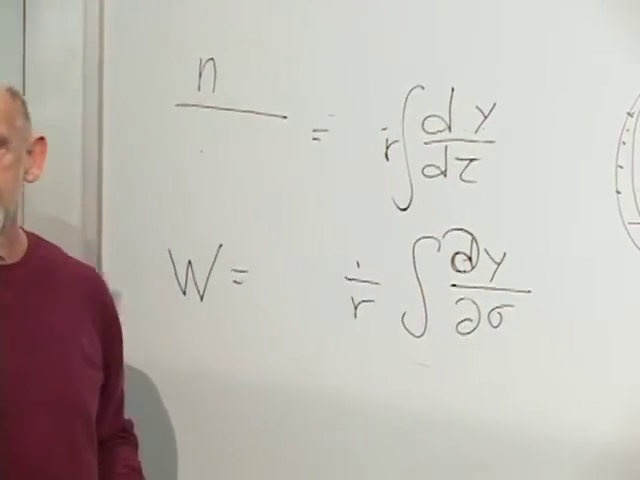
\includegraphics[width=0.72\textwidth]{lecture_10_figure_03.png}
  \medskip

  \begin{tikzpicture}[x=1cm,y=1cm,>=Latex]
    \draw[thick] (-4.0,0.3) circle (0.65);
    \draw[->,thick] (-4.55,0.58) arc (150:-145:0.65);
    \node at (-4.0,-0.65) {$w=+1$};
    \draw[thick] (-2.0,0.3) circle (0.65);
    \draw[->,thick] (-2.55,0.58) arc (150:-145:0.65);
    \node at (-2.0,-0.65) {$w=+1$};
    \node at (-3.0,0.3) {$+$};
    \draw[->,thick] (-1.0,0.3) -- (0.3,0.3);
    \draw[thick] (1.45,0.3) circle (0.78);
    \draw[thick] (1.45,0.3) circle (0.52);
    \draw[->,thick] (0.81,0.74) arc (145:-145:0.78);
    \node at (1.45,-0.78) {$w=+2$};
  \end{tikzpicture}
  \caption{Các số quấn cùng dấu có thể tái nối thành một dây quấn hai lần. Tính liên thông thay đổi trong khi tổng số quấn vẫn là hai.}
  \lectureframe{00:16:40}
  \label{fig:l10-same-winding}
\end{figure}

Sự phân biệt này còn đúng trong mọi quá trình được phép. Tổng số quấn một trăm có thể được mang bởi một dây quấn một trăm vòng, hai dây mỗi dây quấn năm mươi vòng, hoặc một trăm dây mỗi dây quấn một vòng. Các dây có thể tách và nhập giữa các mô tả này, nhưng tổng có dấu vẫn là một trăm. Ta ký hiệu nó bởi \(w\in\mathbb Z\).

\section{Các mode xung lượng và các mode quấn}

Bản thân sự bảo toàn vẫn chưa phải là đối ngẫu. Tiếp theo ta so sánh các năng lượng. Một trạng thái chuyển động quanh đường tròn compact có xung lượng lượng tử hóa
\begin{equation}
  p_Y=\frac{n}{R},
  \qquad n\in\mathbb Z.
  \label{eq:l10-compact-momentum}
\end{equation}
Đối với một trạng thái mà các đóng góp khác vào khối lượng có thể bỏ qua, chuyển động theo phương compact đóng góp \(E_{\rm mom}=|n|/R\). Các giá trị dương và âm của \(n\) biểu thị hai chiều chuyển động ngược nhau, còn năng lượng thì dương.

\begin{figure}[H]
  \centering
  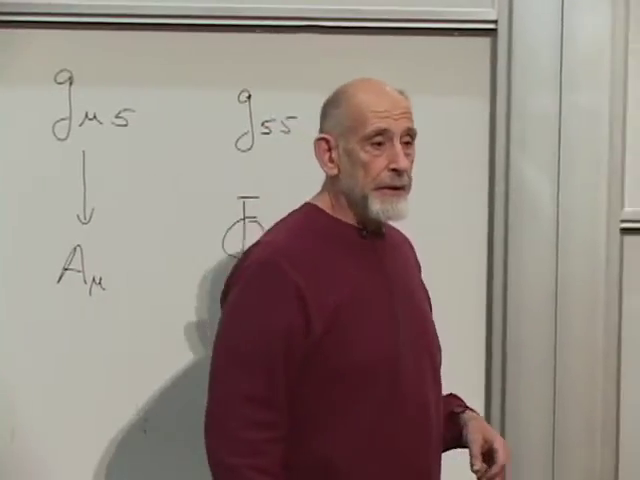
\includegraphics[width=0.72\textwidth]{lecture_10_figure_04.png}
  \caption{Số lượng tử xung lượng compact trên bảng. Bài giảng viết xung lượng một cách sơ đồ như một tích phân của vận tốc theo phương compact.}
  \lectureframe{00:21:30}
  \label{fig:l10-compact-momentum-board}
\end{figure}

Một dây quấn \(|w|\) lần có độ dài \(2\pi |w|R\). Với lực căng của dây cơ bản
\begin{equation}
  T_{\rm F}=\frac{1}{2\pi\alpha'},
\end{equation}
năng lượng quấn của nó là
\begin{equation}
  E_{\rm wind}=T_{\rm F}(2\pi |w|R)
  =\frac{|w|R}{\alpha'}.
  \label{eq:l10-winding-energy}
\end{equation}
Trong đơn vị của bài giảng \(\alpha'=1\), điều này đơn giản là \(E_{\rm wind}=|w|R\).

Hai tháp mức này ứng xử ngược nhau khi bán kính thay đổi. Với \(R\gg
\sqrt{\alpha'}\), các mức xung lượng nằm sít nhau còn các mức quấn thì thưa. Với \(R\ll\sqrt{\alpha'}\), các mức xung lượng thưa còn các mức quấn thì sít nhau.

\begin{figure}[H]
  \centering
  \begin{minipage}[t]{0.48\textwidth}
    \centering
    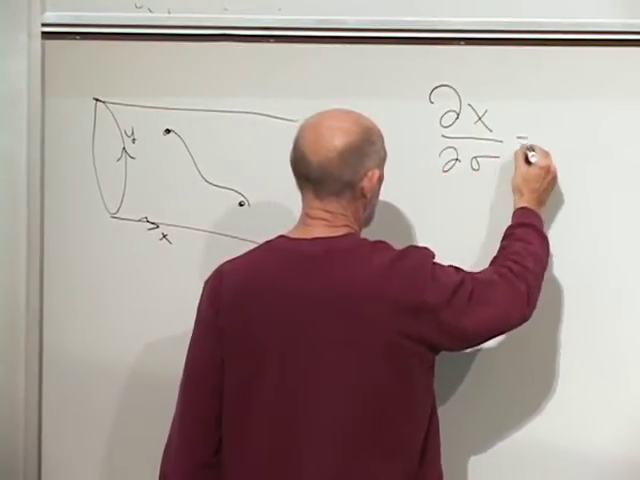
\includegraphics[width=\linewidth]{lecture_10_figure_05.png}
    \par\smallskip
    \textit{Bán kính compact lớn.}
  \end{minipage}\hfill
  \begin{minipage}[t]{0.48\textwidth}
    \centering
    \includegraphics[width=\linewidth]{lecture_10_figure_06.png}
    \par\smallskip
    \textit{Bán kính compact nhỏ.}
  \end{minipage}
  \caption{Hai phép so sánh phổ trên bảng. Các tháp mức thưa và dày đổi vai trò cho nhau khi bán kính được lấy nghịch đảo của nó.}
  \lectureframe{00:25:30--00:26:00}
  \label{fig:l10-dual-spectra-board}
\end{figure}

Sơ đồ gọn nhất là
\begin{figure}[H]
  \centering
  \begin{adjustbox}{max width=\linewidth}
  \begin{tikzpicture}[x=1cm,y=0.74cm,>=Latex]
    \node[font=\bfseries] at (-3.6,6.2) {$R\gg\sqrt{\alpha'}$};
    \draw[->] (-5.1,0) -- (-5.1,5.5) node[above] {$E$};
    \foreach \y in {0.4,1.0,1.6,2.2,2.8,3.4,4.0,4.6}
      \draw (-5.35,\y)--(-4.85,\y);
    \node[align=center] at (-4.25,5.15) {momentum\\dense};
    \draw[->] (-2.2,0) -- (-2.2,5.5) node[above] {$E$};
    \foreach \y in {0.4,2.4,4.4}
      \draw (-2.45,\y)--(-1.95,\y);
    \node[align=center] at (-1.35,5.15) {winding\\sparse};

    \node[font=\bfseries] at (3.6,6.2) {$R\ll\sqrt{\alpha'}$};
    \draw[->] (2.2,0) -- (2.2,5.5) node[above] {$E$};
    \foreach \y in {0.4,2.4,4.4}
      \draw (1.95,\y)--(2.45,\y);
    \node[align=center] at (3.05,5.15) {momentum\\sparse};
    \draw[->] (5.1,0) -- (5.1,5.5) node[above] {$E$};
    \foreach \y in {0.4,1.0,1.6,2.2,2.8,3.4,4.0,4.6}
      \draw (4.85,\y)--(5.35,\y);
    \node[align=center] at (5.95,5.15) {winding\\dense};
  \end{tikzpicture}
  \end{adjustbox}
  \caption{Bản dựng lại của lập luận về khoảng cách mức. Phổ dây đầy đủ không đổi khi hoán đổi xung lượng và số quấn đồng thời với \(R\leftrightarrow\alpha'/R\).}
  \label{fig:l10-dual-spectra-redraw}
\end{figure}

Giả sử một quan sát viên được đưa cho một trong các phổ này mà không được nói nó được tạo ra thế nào. Tháp mức sít nhau là xung lượng trên một đường tròn lớn, hay là quấn trên một đường tròn nhỏ? Chỉ riêng phổ không thể cho biết. Lý thuyết dây đưa ra phát biểu mạnh hơn rằng biên độ tán xạ cũng không thể cho biết. Hai mô tả hoàn toàn tương đương dưới
\begin{equation}
  n\longleftrightarrow w,
  \qquad
  R\longleftrightarrow \widetilde R=\frac{\alpha'}{R}.
  \label{eq:l10-radius-duality}
\end{equation}
Điểm bất động là
\begin{equation}
  R=\sqrt{\alpha'},
  \label{eq:l10-self-dual-radius}
\end{equation}
hay \(R=1\) trong đơn vị của bài giảng. Tại bán kính đó, các trạng thái bổ sung có thể trở nên không khối lượng và đối xứng chuẩn được tăng cường.

\begin{classroomqa}
\audiencequestion{Số quấn có chỉ là một tiện ích toán học để viết lại phổ không? \lecturetimestamp{00:27:33}}
\lecturerresponse{Không. Số quấn gắn nhãn những sector thực của không gian Hilbert dây kín, và những sector đó tham gia vào các tương tác. Từ ``đối ngẫu'' có nghĩa là mô tả xung lượng và mô tả số quấn là hai hệ tọa độ khác nhau của cùng một vật lý, chứ không phải rằng một sector chỉ là một mẹo ghi nhớ tùy chọn cho sector kia.}
\end{classroomqa}

\begin{classroomqa}
\audiencequestion{Có bán kính nào được ánh xạ vào chính nó không?
\lecturetimestamp{00:27:58}}
\lecturerresponse{Có. Giá trị tự đối ngẫu là \(R=\sqrt{\alpha'}\), tức là \(R=1\) trong các đơn vị dùng trên bảng. Hai tháp mức gặp nhau tại đó, và phổ có đối xứng được tăng cường.}
\end{classroomqa}

\section{Dạng worldsheet của đối ngẫu}

Lập luận phổ là gợi ý tốt, nhưng worldsheet làm cho sự hoán đổi trở nên chính xác hơn. Trong chuẩn chỉnh hình, xung lượng liên hợp với \(Y\) tỉ lệ với \(\partial_\tau Y\). Vì vậy tổng xung lượng theo phương compact có dạng
\begin{equation}
  P_Y=\frac{1}{2\pi\alpha'}
      \int_0^{2\pi}d\sigma\,\partial_\tau Y.
  \label{eq:l10-worldsheet-momentum}
\end{equation}
Số quấn là
\begin{equation}
  w=\frac{1}{2\pi R}
      \int_0^{2\pi}d\sigma\,\partial_\sigma Y
   =\frac{Y(2\pi)-Y(0)}{2\pi R}.
  \label{eq:l10-worldsheet-winding}
\end{equation}

\begin{classroomqa}
\audiencequestion{Vì sao tích phân của một đạo hàm lại không triệt tiêu quanh dây kín? \lecturetimestamp{00:32:33}}
\lecturerresponse{Vì \(Y\) là một tọa độ tuần hoàn của không gian đích, chứ không phải một hàm thực đơn trị trên đường tròn \(\sigma\). Điểm worldsheet \(\sigma=2\pi\) là cùng một điểm với \(\sigma=0\), nhưng một phép nâng của phép nhúng lên đường thẳng phủ thay đổi một lượng \(2\pi wR\). Tích phân của \(\partial_\sigma Y\) đo độ dịch đó.}
\end{classroomqa}

\begin{figure}[H]
  \centering
  \includegraphics[width=0.76\textwidth]{lecture_10_figure_07.png}
  \caption{Các tích phân của xung lượng và số quấn sau khi cả hai dòng đã được hoàn tất trên bảng. Các thừa số chung \(2\pi\) và \(\alpha'\) bị lược bỏ trong chuẩn hóa của bài giảng.}
  \lectureframe{00:33:25}
  \label{fig:l10-momentum-winding-integrals}
\end{figure}

Đối với một dây quấn một vòng,
\begin{equation}
  Y(\tau,\sigma+2\pi)=Y(\tau,\sigma)+2\pi R.
\end{equation}
Với số quấn \(w\), độ dịch ở vế phải là \(2\pi wR\). Khi đó phương trình \eqref{eq:l10-worldsheet-winding} đếm chính xác số quấn. Đây là phiên bản chính xác của lối viết tắt trên bảng \(w\sim R^{-1}\int
d\sigma\,\partial_\sigma Y\).

Vì vậy, phát biểu trên worldsheet của đối ngẫu T là
\begin{equation}
  \partial_\tau Y\longleftrightarrow
  \partial_\sigma \widetilde Y,
  \qquad
  \partial_\sigma Y\longleftrightarrow
  \partial_\tau \widetilde Y,
  \label{eq:l10-derivative-duality}
\end{equation}
trong đó xung lượng theo \(Y\) trở thành số quấn trong tọa độ đối ngẫu \(\widetilde Y\), và ngược lại.

\begin{classroomqa}
\audiencequestion{Điều này có nghĩa là bản thân các tọa độ worldsheet \(\tau\) và \(\sigma\) có liên hệ với nhau hay bị hoán đổi cho nhau không?
\lecturetimestamp{00:34:39}}
\lecturerresponse{Không. Đối ngẫu T ánh xạ các nghiệm và hoán đổi những đạo hàm nhất định của tọa độ đích compact. Nó không đồng nhất tọa độ thời gian của worldsheet với tọa độ không gian của worldsheet.}
\end{classroomqa}

\section{Vì sao không thể tránh các trạng thái quấn}

Người ta có thể hỏi vì sao một dây lại có thể được thấy ở trạng thái có quấn khi vẫn có sẵn một trạng thái không quấn. Một dây không chọn trạng thái của nó theo sở thích. Năng lượng được cung cấp trong một va chạm sẽ kéo dãn nó. Một dây đủ năng lượng và bị méo mạnh có thể tái nối thành hai dây có số quấn đối nhau. Tổng số quấn của chúng vẫn bằng không, nhưng sau khi tách ra hai dây có thể rời xa nhau. Một thành viên của cặp có thể bị đưa đi rất xa, để lại cho một quan sát viên một dây có quấn dường như cô lập.

\begin{figure}[H]
  \centering
  \includegraphics[width=0.76\textwidth]{lecture_10_figure_08.png}
  \caption{Một cấu hình có tổng số quấn bằng không nhưng bị kéo dãn mạnh, từ đó các dây có số quấn đối nhau có thể tách ra sau khi tái nối.}
  \lectureframe{00:36:15}
  \label{fig:l10-winding-pair-production}
\end{figure}

Ngưỡng năng lượng được đặt bởi năng lượng quấn. Trên một đường tròn lớn, cần một năng lượng va chạm lớn để kéo đủ chiều dài dây quanh phương compact. Tuy nhiên, một khi vượt ngưỡng, sự tạo cặp quấn--phản quấn không thể bị cấm. Phép tương tự là va chạm photon tạo ra một cặp electron--positron. Tổng điện tích vẫn bằng không, nhưng các hạt mang điện vẫn có mặt và có thể bị tách ra. Bảo toàn số quấn vận hành theo đúng cách đó.

Phép loại suy này không chỉ là bằng lời. Động lượng compact và số quấn hành xử như hai số lượng tử điện tích khác biệt. Trong mô tả rút gọn tương ứng, cùng dấu đẩy nhau và trái dấu hút nhau. Vì vậy, ta nên hỏi hai trường vectơ nào làm trung gian cho các lực đó.

\section{Điện tích động lượng từ hấp dẫn năm chiều}

Hãy bắt đầu với hấp dẫn trong năm chiều. Cho các chỉ số hoa \(M,N\) chạy trên bốn phương không-thời gian thông thường và chiều thứ năm compact. Metric phân rã thành
\begin{equation}
  G_{MN}\quad\longrightarrow\quad
  \bigl\{G_{\mu\nu},\,G_{\mu5},\,G_{55}\bigr\}.
  \label{eq:l10-metric-decomposition}
\end{equation}
Thành phần đối xứng \(G_{5\mu}\) không chứa thông tin mới nào ngoài \(G_{\mu5}\).

\begin{figure}[H]
  \centering
  \includegraphics[width=0.74\textwidth]{lecture_10_figure_09.png}
  \caption{Các nhóm độc lập của các thành phần metric năm chiều: \(G_{\mu\nu}\), \(G_{\mu5}\) và \(G_{55}\).}
  \lectureframe{00:44:05}
  \label{fig:l10-metric-components}
\end{figure}

Từ quan điểm bốn chiều,
\begin{align}
  G_{\mu\nu} &\quad\hbox{is a spacetime metric},\\
  G_{\mu5} &\equiv A_\mu\quad\hbox{is a vector field},\\
  G_{55} &\equiv e^{2\varphi}\quad\hbox{is a scalar modulus}.
  \label{eq:l10-four-dimensional-fields}
\end{align}
Vô hướng \(\varphi\) đo kích thước của chiều compact. Nó có thể biến thiên trơn trên không-thời gian thông thường, nên các sóng của \(\varphi\) là các sóng của bán kính chiều thứ năm.

\begin{figure}[H]
  \centering
  \includegraphics[width=0.74\textwidth]{lecture_10_figure_10.png}
  \caption{Trên bảng, \(G_{\mu5}\) được đồng nhất với một vectơ \(A_\mu\), còn \(G_{55}\) với một vô hướng \(\Phi\).}
  \lectureframe{00:47:40}
  \label{fig:l10-vector-and-radius-modulus}
\end{figure}

Nguồn của một thành phần hấp dẫn hỗn hợp là dòng động lượng hỗn hợp. Cụ thể, động lượng theo chiều thứ năm là nguồn của \(G_{\mu5}\). Vì vậy, một quan sát viên bốn chiều diễn giải số nguyên \(n\) như một điện tích ghép với \(A_\mu\). Đây là cơ chế Kaluza--Klein: cái là động lượng trong hình học số chiều cao hơn trở thành điện tích trong lý thuyết trường số chiều thấp hơn.

\editorialnote{Bài giảng gọi một cách không chặt chẽ vô hướng xuất phát từ \(G_{55}\) là một ``dilaton''. Trong phép rút gọn này, nó cụ thể là môđun bán kính. Dilaton dây mười chiều, trường chi phối hằng số ghép dây, là một trường riêng biệt, mặc dù các tổ hợp vô hướng ở số chiều thấp hơn có thể trộn lẫn dưới các phép đổi khung và đối ngẫu.}

\begin{classroomqa}
\audiencequestion{Vô hướng \(\varphi\) có tỉ lệ với số nguyên động lượng \(n\) không? \lecturetimestamp{00:48:43}}
\lecturerresponse{Không. Số nguyên \(n\) gắn nhãn một trạng thái lượng tử hóa và đóng vai trò điện tích. Vô hướng \(\varphi(x)\) là một trường liên tục quyết định kích thước compact hóa địa phương. Nó có thể thay đổi từ nơi này sang nơi khác; bản thân nó không phải là một số nguyên.}
\end{classroomqa}

\section{Trường vectơ thứ hai và điện tích số quấn}

Số quấn cũng mang tính điện tích, nhưng nó không thể ghép với cùng một vectơ theo cùng cách đó. Để thấy vectơ thứ hai, hãy quay lại các kích thích đầu tiên của dây kín. Một dây kín có các mode dao động tử chuyển trái và chuyển phải. Các trạng thái vật lý tuân theo điều kiện khớp mức: tổng các mức kích thích trái và phải phải bằng nhau.

Trong lý thuyết boson, trạng thái không kích thích là tachyon. Một dao động tử chuyển trái hoặc chuyển phải đơn lẻ sẽ vi phạm điều kiện khớp mức. Vì vậy, trạng thái không khối lượng đầu tiên được phép chứa một dao động tử của mỗi loại,
\begin{equation}
  \alpha_{-1}^{I}\widetilde\alpha_{-1}^{J}\ket{0;k}.
  \label{eq:l10-first-massless-state}
\end{equation}
Các chỉ số \(I,J\) chạy trên các phương không gian ngang, kể cả chiều compact. Nếu một chỉ số là thông thường còn chỉ số kia là \(5\), thì có hai trạng thái dao động tử kiểu vectơ,
\begin{equation}
  \alpha_{-1}^{\mu}\widetilde\alpha_{-1}^{5}\ket{0;k},
  \qquad
  \alpha_{-1}^{5}\widetilde\alpha_{-1}^{\mu}\ket{0;k}.
  \label{eq:l10-two-vector-states}
\end{equation}

\begin{figure}[H]
  \centering
  \includegraphics[width=0.76\textwidth]{lecture_10_figure_11.png}
  \caption{Hai thứ tự dao động tử trái--phải trở thành các trạng thái vectơ bốn chiều khi một phân cực hướng dọc theo chiều compact.}
  \lectureframe{00:58:20}
  \label{fig:l10-two-vector-states-board}
\end{figure}

Các tổ hợp đối xứng và phản đối xứng của chúng thuộc về các trường không-thời gian khác nhau:
\begin{align}
  \alpha_{-1}^{(\mu}\widetilde\alpha_{-1}^{5)}\ket{0;k}
    &\longleftrightarrow G_{\mu5},\\
  \alpha_{-1}^{[\mu}\widetilde\alpha_{-1}^{5]}\ket{0;k}
    &\longleftrightarrow B_{\mu5}.
  \label{eq:l10-g-and-b-vectors}
\end{align}
Trường thứ nhất là vectơ Kaluza--Klein do động lượng compact làm nguồn. Trường thứ hai đi xuống từ trường phản đối xứng Kalb--Ramond và do số quấn của dây làm nguồn. Vì thế, lý thuyết rút gọn chứa hai trường kiểu photon, một cho mỗi loại điện tích.

Nếu cả hai chỉ số dao động tử đều hướng dọc theo chiều compact, thì trạng thái đó là một vô hướng gắn với môđun compact hóa. Nếu cả hai đều nằm trong các phương ngang thông thường, thì phần đối xứng không vết là graviton, phần phản đối xứng là \(B_{\mu\nu}\), và phần vết đóng góp vào một sector vô hướng.

\begin{classroomqa}
\audiencequestion{Trong các trạng thái này, trạng thái nào là singlet và trạng thái nào là triplet? \lecturetimestamp{01:00:21}}
\lecturerresponse{Cách phân loại đó không hữu ích ở đây. Cả hai trạng thái hỗn hợp đều biến đổi như các vectơ bốn chiều. Tổng và hiệu của chúng tách phân cực metric đối xứng khỏi phân cực trường \(B\) phản đối xứng. Trạng thái có hai chỉ số compact thay vào đó là một vô hướng bốn chiều.}
\end{classroomqa}

Bảng đối chiếu đầy đủ thu được trước giờ nghỉ là
\begin{equation}
  \boxed{
  \begin{gathered}
    n\leftrightarrow w,
    \qquad
    R\leftrightarrow\dfrac{\alpha'}{R},\\
    \partial_\tau Y\leftrightarrow\partial_\sigma\widetilde Y,
    \qquad
    G_{\mu5}\leftrightarrow B_{\mu5}.
  \end{gathered}}
  \label{eq:l10-complete-t-duality-map}
\end{equation}

\begin{figure}[H]
  \centering
  \includegraphics[width=0.72\textwidth]{lecture_10_figure_12.png}
  \caption{Bản tóm tắt trên bảng về ánh xạ đối ngẫu T: động lượng và số quấn, bán kính và bán kính nghịch đảo, các đạo hàm trên mặt thế giới, và hai trường vectơ được hoán đổi cho nhau. Giảng viên che khuất một phần dòng cuối, nên dòng đó được bổ sung tường minh trong Phương trình
  \eqref{eq:l10-complete-t-duality-map}.}
  \lectureframe{01:02:20}
  \label{fig:l10-t-duality-map-board}
\end{figure}

Không nên nhầm cách xây dựng này với khẳng định rằng mọi trường vừa liệt kê đều đã được nhận diện trong phổ hạt quan sát được. Ở đây, nó là một hệ quả toán học của lý thuyết dây đã compact hóa. Có nhiều đề xuất nhằm nối những cấu trúc như vậy với hiện tượng học, nhưng đó không phải là bài toán đang được giải trong bài giảng này.

\section{Dây mở làm thay đổi câu hỏi}

Sau giờ nghỉ, ta bắt đầu lại với dây mở. Một dây kín có thể có số quấn bền vì nó không có đầu mút để số quấn có thể tuột mất. Dây mở có các đầu mút nên không có số quấn được bảo vệ tôpô tương tự. Tuy vậy, đối ngẫu T là một đối xứng chính xác của lý thuyết. Đối xứng ấy tác động lên dây mở như thế nào?

Đối với một đầu mút chuyển động tự do, phép biến phân của tác dụng dây cho ra điều kiện biên Neumann. Trong hình học đơn giản \((X,Y)\),
\begin{equation}
  \left.\partial_\sigma X\right|_{\partial\Sigma}=0,
  \qquad
  \left.\partial_\sigma Y\right|_{\partial\Sigma}=0.
  \label{eq:l10-neumann-boundary}
\end{equation}
Bức tranh cơ học thì đơn giản. Hãy xem dây như một chuỗi các phần tử khối lượng ngày càng nhỏ. Một lực tiếp tuyến khác không tác dụng lên phần tử cuối cùng sẽ gây cho nó một gia tốc phân kỳ khi khối lượng của nó tiến tới 0. Vì vậy, một đầu mút tự do sẽ tự điều chỉnh cho tới khi lực căng tổng tại đầu mút triệt tiêu. Dĩ nhiên, ai đó có thể giữ cố định đầu mút và cung cấp lực cần thiết, nhưng khi ấy đầu mút sẽ không còn tự do nữa.

\begin{figure}[H]
  \centering
  \includegraphics[width=0.76\textwidth]{lecture_10_figure_13.png}
  \caption{Dây mở và các điều kiện Neumann tại đầu mút đầy đủ của nó, \(\partial_\sigma X=\partial_\sigma Y=0\).}
  \lectureframe{01:09:20}
  \label{fig:l10-neumann-board}
\end{figure}

Bây giờ chỉ đối ngẫu hóa tọa độ compact \(Y\). Tọa độ không compact \(X\) không đổi. Phương trình \eqref{eq:l10-derivative-duality} biến điều kiện Neumann thứ hai thành
\begin{equation}
  \left.\partial_\tau\widetilde Y\right|_{\partial\Sigma}=0.
  \label{eq:l10-dirichlet-time-derivative}
\end{equation}
Vì vậy, đầu mút có vị trí không đổi theo thời gian trong chiều compact đối ngẫu,
\begin{equation}
  \left.\widetilde Y\right|_{\partial\Sigma}=Y_0.
  \label{eq:l10-dirichlet-boundary}
\end{equation}
Đây là một điều kiện biên Dirichlet.

\begin{figure}[H]
  \centering
  \includegraphics[width=0.76\textwidth]{lecture_10_figure_14.png}
  \medskip

  \begin{adjustbox}{max width=\linewidth}
  \begin{tikzpicture}[x=1cm,y=1cm,>=Latex]
    \node[align=center] at (-3.5,0.8)
      {Neumann\\\(\left.\partial_\sigma Y\right|_{\partial\Sigma}=0\)};
    \draw[->,thick] (-1.7,0.8) -- (1.3,0.8)
      node[midway,above] {$T_Y$};
    \node[align=center] at (3.4,0.8)
      {Dirichlet\\\(\left.\partial_\tau\widetilde Y\right|_{\partial\Sigma}=0\)};
    \node[align=center] at (3.4,-0.5)
      {\(\widetilde Y(\tau)=Y_0\) at each endpoint};
  \end{tikzpicture}
  \end{adjustbox}
  \caption{Điều kiện đầu mút đối ngẫu hoàn chỉnh trên bảng và sự tái dựng logic rõ ràng của nó. Đối ngẫu T biến sự tự do trong chiều compact thành một vị trí đầu mút cố định trong chiều đối ngẫu.}
  \lectureframe{01:12:35}
  \label{fig:l10-neumann-to-dirichlet}
\end{figure}

\begin{classroomqa}
\audiencequestion{Vì sao điều kiện đối ngẫu lại có nghĩa là đầu mút bị cố định? \lecturetimestamp{01:12:39}}
\lecturerresponse{Vì \(\partial_\tau\widetilde Y=0\) có nghĩa là vận tốc bằng 0 theo chiều đã đối ngẫu hóa. Đầu mút bắt đầu ở đâu trong \(\widetilde Y\) thì nó sẽ ở nguyên tại đó. Các tọa độ của nó song song với các phương chưa đối ngẫu hóa vẫn tự do.}
\end{classroomqa}

\section{Vật giữ đầu mút là một D-brane}

Nếu một đầu mút bị cố định, thì phải có cái gì đó giữ được nó tại chỗ. Vì vậy, đối ngẫu T chính xác đòi hỏi một đối tượng mới mà trên đó dây mở có thể tận cùng. Đối tượng ấy là một D-brane. Chữ \(D\) là viết tắt của Dirichlet, không phải của số chiều của đối tượng. Trong phần bình luận lịch sử ngắn của bài giảng, người ta hẳn đã có thể đặt tên các đối tượng này theo Joseph Polchinski, người mà phân tích của ông đã làm cho vai trò động lực học của chúng trở nên hiển nhiên, nhưng thuật ngữ đã có sẵn ``p-brane'' khiến Dirichlet trở thành tên gọi tự nhiên.

Một \(p\)-brane có \(p\) chiều không gian. Dây là một one-brane, màng là một two-brane, và một vật thể kéo dài ba chiều là một three-brane. Một D\(p\)-brane là một \(p\)-brane mà trên đó các đầu mút của dây cơ bản tuân theo điều kiện Dirichlet trong các phương ngang và điều kiện Neumann trong các phương tiếp tuyến với brane.

Không có gì trong lập luận đối ngẫu chọn riêng một giá trị nào của \(Y_0\), nên D-brane không thể là một vật cố định cứng bị đóng đinh tại một điểm ưu tiên nào đó trong vũ trụ. Nó phải có thể di chuyển được. Thuyết tương đối cũng cấm một vật thể kéo dài tuyệt đối cứng, nên một D-brane có thể dao động và uốn cong. Brane phẳng đơn giản được vẽ trên bảng là cấu hình cân bằng của nó, không phải một sự hạn chế đối với động lực học của nó.

\begin{classroomqa}
\audiencequestion{Hai đầu mút của một dây mở có nhất thiết phải có cùng một giá trị cố định của tọa độ đối ngẫu không? \lecturetimestamp{01:14:55}}
\lecturerresponse{Nói chung là không. Cả hai đầu mút có thể nằm trên cùng một D-brane, trong trường hợp đó chúng chia sẻ cùng vị trí ngang của brane ấy. Chúng cũng có thể nằm trên hai D-brane khác nhau ở các vị trí ngang khác nhau, và khi đó dây sẽ căng giữa chúng. Bản thân brane cũng có thể dao động và uốn cong, nên quỹ tích đầu mút không nhất thiết phải luôn là một mặt phẳng hoàn toàn phẳng.}
\end{classroomqa}

\section{Đếm số chiều của một D-brane}

Lý thuyết siêu dây mười chiều có chín chiều không gian. Giả sử đối ngẫu T áp đặt một điều kiện Dirichlet theo một phương không gian. Đầu mút vẫn tự do trong tám phương còn lại, nên quỹ tích được phép của nó là một D8-brane tám chiều. Mỗi điều kiện Dirichlet độc lập bổ sung loại bỏ một phương chuyển động của đầu mút. Nếu \(k\) tọa độ không gian bị cố định, thì
\begin{equation}
  p=9-k.
  \label{eq:l10-dp-counting}
\end{equation}

Ví dụ mặt bàn cho phiên bản ba chiều của cùng phép đếm ấy. Cố định tọa độ thẳng đứng thì đầu ngón tay có thể di chuyển trên một mặt bàn hai chiều. Cố định thêm tọa độ thứ hai thì nó chỉ có thể di chuyển dọc theo một đường thẳng. Cố định cả ba thì nó bị giam tại một điểm.

\begin{figure}[H]
  \centering
  \begin{adjustbox}{max width=\linewidth}
  \begin{tikzpicture}[x=1.05cm,y=1cm,>=Latex]
    \draw[fill=blue!8] (-5.5,-0.7) -- (-2.5,-0.7) -- (-1.7,0.2)
      -- (-4.7,0.2) -- cycle;
    \node at (-3.6,-1.15) {one constraint: sheet};
    \draw[very thick,blue!60!black] (-0.9,-0.25) -- (1.3,-0.25);
    \node at (0.2,-1.15) {two constraints: line};
    \fill[blue!70!black] (4.1,-0.25) circle (0.09);
    \node at (4.1,-1.15) {three constraints: point};
    \draw[->] (-1.45,0.95) -- (-0.75,0.95);
    \draw[->] (2.25,0.95) -- (2.95,0.95);
    \node at (0.35,1.35) {each Dirichlet condition lowers \(p\) by one};
  \end{tikzpicture}
  \end{adjustbox}
  \caption{Lập luận đếm số chiều được dùng trong ví dụ mặt bàn. Một D\(p\)-brane là quỹ tích trong đó các đầu mút vẫn tự do chuyển động.}
  \label{fig:l10-dp-counting-redraw}
\end{figure}

Các phép đối ngẫu lặp lại sinh ra các D8-, D7-, D6-brane, v.v., cho tới một D0-brane, là một đối tượng dạng điểm trong không gian. Nếu không có phương không gian nào bị cố định, thì một D9-brane chiếm trọn cả chín chiều không gian và các dây mở thông thường tự do di chuyển khắp nơi. Bài giảng có nhắc ngắn gọn đến các D\((-1)\)-brane; chúng khu trú trong không-thời gian Euclid và hành xử như instanton hơn là như các hạt thông thường lan truyền theo thời gian.

\editorialnote{Bậc thang số chiều là một phát biểu về hai lý thuyết loại II khi xét chung. Các D\(p\)-brane BPS bền có \(p\) chẵn trong type IIA và \(p\) lẻ trong type IIB. Đối ngẫu T dọc theo một đường tròn làm thay đổi \(p\) đi một đơn vị và đồng thời trao đổi type IIA với type IIB.}

\begin{classroomqa}
\audiencequestion{Nếu chỉ có sáu chiều là compact, thì phép đếm có nên bắt đầu bằng cách trừ từ sáu thay vì từ chín không? \lecturetimestamp{01:20:49}}
\lecturerresponse{Phép suy ra sơ cấp thực hiện đối ngẫu T trên các phương compact, nhưng một đường tròn đối ngẫu trở nên lớn tùy ý khi đường tròn ban đầu trở nên nhỏ tùy ý. Trong giới hạn đó, nó hiệu dụng là không compact. Vì thế, các brane thu được có thể kéo dài dọc theo hoặc vuông góc với những phương mà ở các thang đo có thể tiếp cận trông như không compact. Số chiều \(p\) đếm tất cả các phương không gian tiếp tuyến với brane, chứ không chỉ các phương compact được dùng trong một phép suy ra.}
\end{classroomqa}

Một D0-brane là một loại hạt mới. Một dây mở có thể nối từ một D0-brane sang một brane khác, quay về chính D0-brane đó, hoặc kéo dài về phía một brane ở rất xa. Nếu hiểu theo nghĩa đen là kéo ra vô cực không gian thì một dây có độ dài vô hạn và do đó năng lượng vô hạn, vì vậy phiên bản hữu ích về mặt vật lý đặt đầu mút còn lại của nó trên một đối tượng khác.

Trường hợp tiếp theo, D1-brane, bản thân nó có dạng sợi dây, nhưng không phải là dây cơ bản mà ta đã bắt đầu với. Nó có thể uốn cong và khép lại trên chính nó, và các dây cơ bản có thể kết thúc trên nó. Sức căng của nó biến thiên theo hằng số liên kết dây theo một cách khác:
\begin{equation}
  T_{\rm D1}=\frac{1}{2\pi\alpha' g_s},
  \qquad
  T_{\rm F1}=\frac{1}{2\pi\alpha'}.
  \label{eq:l10-dstring-tension}
\end{equation}
Ở chế độ liên kết yếu \(g_s\ll1\), D-dây nặng hơn nhiều so với dây cơ bản, điều này giải thích vì sao ban đầu nó xuất hiện như một điểm neo có khối lượng lớn.

\begin{figure}[H]
  \centering
  \includegraphics[width=0.76\textwidth]{lecture_10_figure_15.png}
  \caption{D1-brane trên bảng: một đối tượng một chiều có thể uốn cong, khác với các dây cơ bản có thể kết thúc trên nó.}
  \lectureframe{01:24:20}
  \label{fig:l10-d1-brane}
\end{figure}

\begin{classroomqa}
\audiencequestion{Đối ngẫu T có tác động lên các D-brane cũng như lên các dây không? \lecturetimestamp{01:25:35}}
\lecturerresponse{Có. Một phép đối ngẫu T theo một phương song song với một D\(p\)-brane làm hạ số chiều của nó xuống D\((p-1)\), còn một phép đối ngẫu T theo một phương trực giao với nó làm tăng số chiều lên D\((p+1)\). Các brane là một phần của từ điển đối ngẫu, chứ không phải những giá đỡ bên ngoài vẫn giữ nguyên dưới phép đó.}
\end{classroomqa}

\begin{classroomqa}
\audiencequestion{Các phương tiếp tuyến với một brane vẫn có thể là compact chứ?
\lecturetimestamp{01:27:25}}
\lecturerresponse{Có. ``Tiếp tuyến'' và ``compact'' trả lời những câu hỏi khác nhau. Một phương có thể nằm dọc theo brane mà vẫn khép thành một đường tròn; nó cũng có thể là không compact. Điều quan trọng đối với đầu mút là điều kiện biên theo phương đó là Neumann hay Dirichlet.}
\end{classroomqa}

Một D2-brane là một tấm dạng màng. Một D3-brane có ba chiều không gian. Trong một không-thời gian thực sự nhiều chiều hơn, một D3-brane là một không gian con ba chiều chứ không phải toàn bộ không gian, mặc dù những quan sát viên bị giới hạn trên nó có thể trải nghiệm nó như toàn bộ thế giới không gian của mình.

\begin{figure}[H]
  \centering
  \includegraphics[width=0.76\textwidth]{lecture_10_figure_16.png}
  \caption{Một D2-brane được vẽ như một tấm mà trên đó các đầu mút dây có thể chuyển động.}
  \lectureframe{01:27:55}
  \label{fig:l10-d2-brane}
\end{figure}

Phép suy ra trình bày ở đây cố ý chỉ là một phác thảo. Tự nó không phải là bằng chứng rằng lý thuyết dây mô tả tự nhiên. Tuy nhiên, bên trong lý thuyết dây, các kiểm tra nhất quán là rất nhiều: các đối ngẫu, các tính toán lượng tử và các kết quả toán học đều chỉ ra rằng D-brane là những đối tượng động lực học đích thực.

\section{Các dây mở trở thành các trường trên một brane}

Hãy lấy một D2-brane vốn trống và đặt lên nó các dây mở ngắn. Mỗi đầu mút bị giới hạn trên tấm đó, nên toàn bộ kích thích năng lượng thấp chuyển động dọc theo tấm. Hai dây có định hướng mà các đầu mút kề nhau mang các mũi tên tương thích có thể nối lại. Dây đã nối về sau có thể lại tách ra. Nếu đọc như lịch sử của các hạt, thì đây là các đỉnh của giản đồ Feynman: hai hạt đi vào, một kích thích trung gian lan truyền, và hai hạt đi ra.

\begin{figure}[H]
  \centering
  \includegraphics[width=0.76\textwidth]{lecture_10_figure_17.png}
  \caption{Các dây mở có định hướng trên một D2-brane nối với nhau qua các đầu mút tương thích. Ở năng lượng thấp, quá trình này được hiểu như một tương tác lý thuyết trường trên brane.}
  \lectureframe{01:29:55}
  \label{fig:l10-open-strings-on-brane}
\end{figure}

Ở các năng lượng thấp hơn nhiều so với thang dây, tháp các mode dao động nội tại không được kích thích. Trạng thái dây mở không khối lượng còn lại là một trường vectơ trên thể tích thế giới của brane. Với một brane, đó là một trường chuẩn abel \(U(1)\), tương tự điện từ học trên brane. Trường ấy không lan truyền trong toàn bộ không gian khối mười chiều; các lượng tử của nó là những dây mở mà các đầu mút giữ chúng trên brane.

\section{Một chồng brane tạo ra màu không abel}

Bây giờ hãy đặt vài brane song song ở gần nhau. Với ba brane, hãy gán nhãn chúng là Red, Green và Blue. Một dây có định hướng mang một cặp có thứ tự gồm các nhãn đầu mút: nó có thể đi từ Red đến Green, từ Green đến Blue, từ Red đến Red, v.v. Với \(N\) brane, các trạng thái dây mở không khối lượng có thể được sắp thành một ma trận \(N\times N\)
\begin{equation}
  A_\mu{}^{i}{}_{j},
  \qquad i,j=1,\ldots,N.
  \label{eq:l10-chan-paton-matrix}
\end{equation}
Đó là các nhãn Chan--Paton của một lý thuyết chuẩn \(U(N)\).

\begin{figure}[H]
  \centering
  \includegraphics[width=0.76\textwidth]{lecture_10_figure_18.png}
  \medskip

  \begin{adjustbox}{max width=\linewidth}
  \begin{tikzpicture}[x=1cm,y=1cm,>=Latex]
    \draw[very thick,red!70!black] (-4.8,2.0)--(4.8,2.0);
    \draw[very thick,green!55!black] (-4.8,0.8)--(4.8,0.8);
    \draw[very thick,blue!70!black] (-4.8,-0.4)--(4.8,-0.4);
    \node[left] at (-4.8,2.0) {Red};
    \node[left] at (-4.8,0.8) {Green};
    \node[left] at (-4.8,-0.4) {Blue};
    \draw[->,thick] (-3.4,2.0) .. controls (-2.8,1.35) and (-2.3,1.15)
      .. (-1.7,0.8);
    \node at (-2.7,1.05) {$R\!G$};
    \draw[->,thick] (-0.6,0.8) .. controls (0.0,0.25) and (0.6,-0.05)
      .. (1.2,-0.4);
    \node at (0.1,0.0) {$G\!B$};
    \draw[->,thick] (2.1,2.0) .. controls (2.9,2.55) and (3.8,2.55)
      .. (4.3,2.0);
    \node at (3.2,2.65) {$R\!R$};
  \end{tikzpicture}
  \end{adjustbox}
  \caption{Ba brane song song trên bảng và cách dựng lại rõ ràng các nhãn đầu mút có thứ tự do những dây giữa chúng mang.}
  \lectureframe{01:33:15}
  \label{fig:l10-three-brane-stack}
\end{figure}

\begin{classroomqa}
\audiencequestion{Một dây có thật sự thể chạy từ brane Red đến brane Green mà không bị các hình vẽ khác chặn lại không? \lecturetimestamp{01:35:07}}
\lecturerresponse{Có. Các brane được nhúng trong một không gian nhiều chiều hơn. Hình vẽ hai chiều trên bảng chỉ là một phép chiếu, nên một dây có thể đi vòng qua một đường được chiếu khác theo một phương trực giao.}
\end{classroomqa}

\begin{classroomqa}
\audiencequestion{Một dây Red--Green có bắt buộc phải ghép với một dây Green--Blue để trở thành Red--Blue không? \lecturetimestamp{01:35:39}}
\lecturerresponse{Đó là quy tắc nối cục bộ cơ bản. Các đầu mút tương thích gặp nhau, và hai đoạn trở thành một dây duy nhất mà các đầu mút chưa nối của nó giữ lại các nhãn Red và Blue. Những quá trình phức tạp hơn được xây dựng bằng cách lặp lại cùng phép đó.}
\end{classroomqa}

Quy tắc nối là phép nhân ma trận được hình học hóa. Một dây Red--Green có thể nối với một dây Green--Blue vì đầu mút Green của cái này tương thích với đầu mút Green của cái kia. Kết quả là một dây Red--Blue:
\begin{equation}
  (R,G)\circ(G,B)\longrightarrow(R,B).
  \label{eq:l10-color-composition}
\end{equation}
Chỉ số lặp được nối lại và biến mất ở bên trong. Đây chính là cùng một cấu trúc chỉ số xuất hiện tại một đỉnh tương tác Yang--Mills.

\begin{figure}[H]
  \centering
  \includegraphics[width=0.76\textwidth]{lecture_10_figure_19.png}
  \caption{Sự nối các dây mở trên một chồng brane. Định hướng đầu mút áp đặt cùng phép hợp thành chỉ số có thứ tự như phép mà các trường chuẩn không abel sử dụng.}
  \lectureframe{01:36:30}
  \label{fig:l10-color-joining-board}
\end{figure}

Đối với ba brane trùng nhau, nhóm chuẩn dây mở đầy đủ là \(U(3)\), với chín trạng thái vectơ. Đại số của nó phân rã thành
\begin{equation}
  \mathfrak u(3)=\mathfrak{su}(3)\oplus\mathfrak u(1).
  \label{eq:l10-u3-decomposition}
\end{equation}
Tám tổ hợp không vết mang cấu trúc màu của các gluon QCD, còn thành phần \(U(1)\) đường chéo của khối tâm là một trường abel riêng biệt.

\editorialnote{Bài giảng mô tả một trong chín tổ hợp cặp màu như có thể tách ra và biến mất, qua đó còn lại tám gluon. Phát biểu D-brane chính xác là một chồng ba brane trùng nhau cho \(U(3)\), chứ không chỉ \(SU(3)\). Để thu được bát tuyến QCD, cần tách riêng, chiếu bỏ, hoặc bằng cách khác khử liên kết \(U(1)\) đường chéo. Hình minh họa trong bài giảng đúng ở chỗ gợi ra các chỉ số màu có thứ tự, nhưng không phải là một suy dẫn đầy đủ của QCD.}

Vật chất kiểu quark chỉ mang một chỉ số màu. Trong bức tranh brane, nó được biểu diễn bởi một dây có một đầu mút trên chồng màu và đầu kia trên một brane khác ở xa. So với chồng màu, chỉ một đầu hiện ra như một nhãn màu. Đảo ngược định hướng cho ra phản hạt. Một dây kiểu quark và một dây kiểu phản quark với các đầu mút tương thích có thể nối lại rồi rời khỏi chồng màu; hai dây kiểu quark có cùng định hướng thì không thể hủy nhau theo cách đó.

Các lý thuyết năng lượng thấp thu được nói chung là các lý thuyết Yang--Mills siêu đối xứng, với vật chất bổ sung được xác định bởi các brane và các giao nhau của chúng. Chúng đủ gần với QCD để làm sáng tỏ động lực học không abel, nhưng không tự động là Mô hình Chuẩn. Chỉ với một brane, cùng phép xây dựng ấy rút xuống thành một lý thuyết \(U(1)\): các dây ngắn brane--brane giống photon, còn các dây có định hướng vươn tới một sector thứ hai đóng vai trò của điện tích dương và âm.

\section{D-dây kết thúc như các đơn cực từ}

Giờ đây trong câu chuyện có hai loại đối tượng dạng dây. Dây cơ bản ban đầu, hay F-dây, mang thông lượng điện trên một D3-brane. D1-brane, hay D-dây, nặng hơn nhiều ở liên kết yếu. Một D-dây cũng có thể kết thúc trên một D3-brane. Đầu mút của nó không mang điện tích điện dưới trường chuẩn trên thể tích thế giới; nó mang điện tích từ. Từ góc nhìn của các quan sát viên trên D3-brane, đầu mút ấy là một đơn cực từ.

\begin{figure}[H]
  \centering
  \includegraphics[width=0.76\textwidth]{lecture_10_figure_20.png}
  \medskip

  \begin{adjustbox}{max width=\linewidth}
  \begin{tikzpicture}[x=1cm,y=1cm,>=Latex]
    \draw[fill=blue!7] (-3.8,-0.5)--(2.6,-0.5)--(3.6,0.35)--(-2.8,0.35)--cycle;
    \node at (2.25,-0.95) {D3-brane};
    \draw[very thick,red!70!black] (0.0,3.0)--(0.0,0.0);
    \fill[black] (0.0,0.0) circle (0.08);
    \node[right] at (0.15,2.1) {D-string};
    \foreach \a in {25,65,115,155} {
      \draw[->,blue!65!black] (0.0,0.0)--({1.25*cos(\a)},{0.65*sin(\a)});
    }
    \node[align=center] at (4.8,1.7) {magnetic flux\\on the D3 worldvolume};
    \draw[->] (3.7,1.35)--(1.05,0.45);
  \end{tikzpicture}
  \end{adjustbox}
  \caption{Cấu hình đầu mút trên bảng và cách diễn giải rõ ràng của nó. Một D-dây kết thúc trên một D3-brane xuất hiện như một đơn cực từ đối với lý thuyết chuẩn trên thể tích thế giới.}
  \lectureframe{01:41:30}
  \label{fig:l10-dstring-monopole}
\end{figure}

Phân cấp khối lượng cũng có dạng định tính đúng. Vì sức căng của D-dây mang một thừa số \(1/g_s\), đầu mút của nó nặng hơn nhiều so với một kích thích điện thông thường ở liên kết yếu. Quan hệ điện/từ giữa các đầu mút của F-dây và D-dây là một phần của cấu trúc đối ngẫu rộng hơn của lý thuyết dây loại IIB.

\begin{classroomqa}
\audiencequestion{Đầu mút của D-dây có trung hòa không?
\lecturetimestamp{01:42:19}}
\lecturerresponse{Nó trung hòa đối với điện tích điện do đầu mút của dây cơ bản mang, nhưng không phải là không mang điện tích. Nó mang điện tích từ và vì thế là một đơn cực trong lý thuyết chuẩn trên D3-brane.}
\end{classroomqa}

\section{Phép xây dựng này khẳng định điều gì và không khẳng định điều gì}

Con đường từ đối ngẫu T đến các brane được ghép lại trong nhiều thập niên, chứ không phải trong một phép tính đơn lẻ. Một lý thuyết ban đầu được đề xuất để mô tả các hadron đã trở thành một lý thuyết ứng viên của hấp dẫn lượng tử. Các đối ngẫu của nó sau đó buộc D-brane phải xuất hiện trong phổ, và các lý thuyết chuẩn lại tái xuất hiện như động lực học năng lượng thấp của những dây kết thúc trên các brane ấy. Theo nghĩa đó, chủ đề này đã đi trọn một vòng.

D-brane và các cấu trúc đối ngẫu liên quan đã trở thành những công cụ mạnh để nghiên cứu các lý thuyết chuẩn siêu đối xứng, các hệ liên kết mạnh, và các mối liên hệ giữa hấp dẫn với lý thuyết trường. Chúng cũng đã cung cấp hiểu biết cho các mô hình chất lưu và plasma thông qua đối ngẫu chuẩn/hấp dẫn. Thành công này không đồng nghĩa với việc suy ra trực tiếp phổ hạt quan sát được. Hình học compact hóa, cấu hình brane, sự phá vỡ siêu đối xứng và nhiều thành phần khác vẫn còn phải được lựa chọn.

\begin{classroomqa}
\audiencequestion{Điều gì quyết định chiều compact nào được đối ngẫu hóa?
\lecturetimestamp{01:44:59}}
\lecturerresponse{Về mặt toán học, ta có thể đối ngẫu hóa bất kỳ phương compact nào mà đối xứng cần thiết hiện diện, và chọn mô tả thuận tiện nhất. Về mặt vật lý, các định hướng brane và dữ liệu compact hóa được hiện thực trong một trạng thái cụ thể được lựa chọn bởi lịch sử và động lực học của trạng thái đó.}
\end{classroomqa}

\begin{classroomqa}
\audiencequestion{Brane nào mang phép xây dựng đơn cực này?
\lecturetimestamp{01:45:21}}
\lecturerresponse{Thế giới mà lý thuyết chuẩn sống trên đó là một D3-brane. D-dây kéo dài theo một phương trực giao và kết thúc trên D3-brane đó; đầu mút của nó là đơn cực được thấy trong ba chiều không gian của brane.}
\end{classroomqa}

\begin{classroomqa}
\audiencequestion{D-dây cũng có định hướng chứ?
\lecturetimestamp{01:45:55}}
\lecturerresponse{Có. Đảo ngược định hướng của một D-dây sẽ đảo ngược điện tích tương ứng. Hai định hướng đầu mút phân biệt đơn cực với phản đơn cực, cũng như định hướng phân biệt điện tích điện đối với các đầu mút của dây cơ bản.}
\end{classroomqa}

\begin{classroomqa}
\audiencequestion{Bức tranh xuyến đơn giản này có thể giải thích bất đối xứng trái--phải của vật lý hạt chiral không?
\lecturetimestamp{01:46:05}}
\lecturerresponse{Tự nó thì không. Một xuyến phẳng quá đối xứng. Các phổ chiral đòi hỏi nhiều cấu trúc hơn, chẳng hạn các giao nhau brane bất đối xứng, các phép chiếu orbifold, hoặc compact hóa trên các hình học Calabi--Yau thích hợp. Lý thuyết dây có những cơ chế cho tính chiral, nhưng chúng nằm ngoài phép xây dựng đối ngẫu T sơ cấp này.}
\end{classroomqa}

Chúng ta đã theo dõi một đối xứng qua bốn dạng biểu hiện cụ thể:
sự hoán đổi các phổ, sự hoán đổi các đạo hàm trên mặt thế giới, sự hoán đổi
các trường không-thời gian, và cuối cùng là sự hoán đổi các điều kiện biên
ở đầu mút. Dạng cuối cùng mới là dạng mang tính quyết định. Nó biến một sự
tương đương toán học thành việc khám phá ra các D-brane, và biến động lực
học của dây mở thành lý thuyết chuẩn trên các thể tích thế giới của chúng.
Đến lúc đó, theo cách nói của Susskind, bài giảng đã dùng hết thời gian,
năng lượng và xung lượng của nó.

\end{document}